\documentclass[12pt,a4paper]{article}
\usepackage[utf8]{inputenc}
\usepackage[T1]{fontenc}
\usepackage{amsmath}
\usepackage{amssymb}
\usepackage{graphicx} %Used for photos
\usepackage{float} %Used for inline figures
\usepackage{bbm} % Used for indicator function
\usepackage{enumitem} % Used for enumerate w/ \alpha or roman
\usepackage{hyperref} % Used for links, such as table of contents links

\title{Probability and Measure Solutions}
\author{WispyAbyss}

% Math operators

% Definitions
\newcommand{\inner}[2]{\left\langle #1 , #2 \right\rangle}
\newcommand{\norm}[1]{\left\|#1\right\|}
\newcommand{\1}[1]{\mathbbm{1}\left\{ #1 \right\}}
\newcommand{\R}{\mathbb{R}}
\newcommand{\N}{\mathbb{N}}
\newcommand{\E}{\mathbb{E}}
\newcommand{\F}{\mathcal{F}}
\newcommand{\Z}{\mathbb{Z}}
\newcommand{\Q}{\mathbb{Q}}
\newcommand{\acal}{\mathcal{A}}
\newcommand{\ical}{\mathcal{I}}
\newcommand{\lcal}{\mathcal{L}}
\newcommand{\ucal}{\mathcal{U}}
\newcommand{\tcal}{\mathcal{T}}
\newcommand{\dcal}{\mathcal{D}}
\newcommand{\fcal}{\mathcal{F}}
\newcommand{\bcal}{\mathcal{B}}
\newcommand{\gcal}{\mathcal{G}}
\newcommand{\hcal}{\mathcal{H}}
\newcommand{\mcal}{\mathcal{M}}
\newcommand{\pcal}{\mathcal{P}}
\newcommand{\Prob}{\mathbb{P}}
\newcommand{\VCdim}{\text{VCdim}}
\newcommand{\st}{\text{s.t.}}
\newcommand{\roundUp}[1]{\left\lceil #1 \right\rceil}
\newcommand{\roundDown}[1]{\left\lfloor #1 \right\rfloor}
\newcommand{\sign}{\text{sign}}
\newcommand{\ceil}[1]{\left\lceil#1\right\rceil}
\newcommand{\floor}[1]{\left\lfloor #1 \right\rfloor}
\renewcommand{\div}{\text{div}}
\newcommand{\curl}{\text{curl}}
\newcommand{\trace}{\text{trace}}
\newcommand{\grad}{\text{grad}}
\newcommand{\io}{\text{i.o.}}


\setcounter{secnumdepth}{0}

\begin{document}
\maketitle
	
\tableofcontents
	
\section{Forward}
This document will contain notes and solutions corresponding to Probability and Measure, Third Edition, by Patrick Billingsley  [\href{https://www.amazon.com/PROBABILITY-MEASURE-WILEY-MATHEMATICAL-STATISTICS/dp/8126517719/ref=sr_1_2?crid=3IVF52UANVNQC&keywords=Probability+and+Measure+by+Patrick+Billingsley&qid=1694149664&s=books&sprefix=probability+and+measure+by+patrick+billingsley%2Cstripbooks%2C143&sr=1-2}{amazon}].
\\\\
A note on how I will do the questions. I want to answer every question, but there really are a lot of them. So, I think I will tackle them this way. To get through a chapter, I'll go through every question that is in the back of the book (as they are the most important, and might be needed at a later time). Then, I'll go maybe over 3-4 more. Then, I'll answer one question I skipped from the previous chapters.

\section{Section 1 - Borel's Normal Number Theorem}
\subsection{Notes}
For a complete understanding of probability, you need to understand an infinite number of events as well as a finite number of events. We try and present why that must be so here.

\subsubsection{The Unit Interval} 
We take the length of an interval $I = (a,b] = b - a$. Note, for $A$ a disjoint set of intervals in $(0,1]$, we have that $P(A)$ is well defined. If $B$ is a similar disjoint set, and is disjoint from $A$, $P(A + B) = P(A) + P(B)$ is well defined as well. Note - we haven't defined anything for intersections yet. These definitions can also directly stem from the Riemann integral of step functions.
\\\\
The unit interval can give the probability that a single particle is emitted in a unit interval of time. Or a single phone call comes in. However, it can also model an infinite coin toss. This is done as follows - for $\omega \in (0,1]$, define:
$$
	\omega = \sum_{n=1}^\infty \frac{d_n(\omega)}{2^n}
$$
Where $d_n(\omega)$ is $0$ or $1$, and comes from the binary expansion of $\omega$. We take $\omega$ as the non terminating representation. Note, we were particular when we defined intervals as half inclusive. Examine the set of $\omega$ for which $d_i(\omega) = u_i$ for $i = 1, \cdots, n$, $u_i \in \{0,1\}$. We have that:
$$
	\sum_{i=1}^n \frac{u_i}{2^i} < \omega \leq \sum_{i=1}^n \frac{u_i}{2^i} + \sum_{i=n+1}^\infty \frac{1}{2^i}
$$
We cannot have the lower extreme value, as this would imply $\omega$ takes on its terminating binomial representation, which is what we said we would not do. This is our first taste, I guess, of measure $0$ sets, we we still have:
$$
	\Prob\left[\omega: d_i(\omega) = u_i, i = 1, \cdots, n \right] = \frac{1}{2^n}
$$
Note, probabilities of various familiar events can be written down immediately. Ultimately, note, however, each probability is the sum of disjoint dyadic intervals of various ranks $k$. Ie, all the events are still well defined by our probability definition above. We have:
$$
	\Prob\left[\omega : \sum_{i=1}^n d_i(\omega) = k\right] = {n \choose k} \frac{1}{2^n}
$$
All these results have been for finitely many components of $d_i(\omega)$. What we are interested in, however, is properties of the entire sequence of $\omega = (d_1(\omega), d_2(\omega), \cdots)$. 

\subsubsection{The Weak Law of Large Numbers}
What I like about this chapter, is to me - it \textit{emphasizes} the connection between the \textit{structure of real numbers}, and probability. At the end of the day - probability can be seen as just extracting properties of \textit{frequency} over the real numbers, to be understood as probabilistic statements. However, with just our basic real numbers - we can't really prove a lot of properties about infinite things. That is when measure theory comes in later. However, for now, we look at what we can prove - and that starts with the weak law of large numbers. We have:

\paragraph{Theorem 1.1 - The Weak Law of Large Numbers} For each $\epsilon$:
$$
	\lim_{n \to \infty} \Prob\left[
	\omega: \left|\frac{1}{n}\sum_{i=1}^n d_i(\omega) - \frac{1}{2}\right| \geq \epsilon
	\right] = 0
$$
Probabilistically - this is saying that if $n$ is large, then there is a small probability that the fraction/relative \textit{frequency} of heads in $n$ tosses will deviate much from $1/2$. Think about it as a statement over the real numbers as well - it is also interesting. Ultimately, the intervals containing $\omega$ that do not satisfy the above are getting smaller and smaller and smaller. We formalize this with the following concept:
\\\\
As $d_i(\omega)$ are constant over each dyadic interval of rank $n$ if $i \leq n$, the sums $\sum_{i=1}^n d_i(\omega)$ are also constant over rank $n$. Thus, the set in the theorem is just a disjoint union of dyadic intervals of rank $n$. Note - the theorem is saying, that the total weight given to those intervals gets smaller and smaller as $n$ goes to infinity.
\\\\
Now, we go over how to prove the theorem. It relies on rademacher variables:
$$
	r_n(\omega) = 2d_n(\omega) - 1
$$
These are $\pm 1$ when $d_n = 1/0$. Note, these have the same "being constant on dyadic intervals" properties as $d_n(\omega)$. We define:
$$
	s_n(\omega) = \sum_{i=1}^n r_i(\omega)
$$
And so, our theorem is equivalent to proving:
$$
	\lim_{n \to \infty} \Prob\left[
	\omega: \left|\frac{1}{n} s_n(\omega)\right| \geq \epsilon
	\right] = 0
$$
Note, rademacher functions also have interpretations, probabilistically, of random walks and such. With these variables, we can ultimately find properties, going all the way to:
$$
	\int_0^1 s_n^2(\omega) = n
$$
However, what interests me is the following: Chebyshev's Lemma, but as a property of the real numbers. We have:

\paragraph{Lemma - Chebyshev's Inequality} If $f$ is a nonnegative step function, then $[\omega: f(\omega) \geq \alpha]$ is for $\alpha > 0$ a finite union of intervals, and:
$$
	\Prob\left[\omega: f(\omega) \geq \alpha\right] \leq \frac{1}{\alpha} \int_0^1 f(\omega) d\omega
$$
Proof: Note, it is all just properties of step functions. Let $c_j$ correspond to the step intervals $(x_{j-1},x_j]$, and let $\sum'$ be the sum over $c_j \geq \alpha$. Then, we have quite easily:
$$
	\int_0^1 f(\omega) d\omega =
	\sum c_j (x_j - x_{j-1}) \geq 
	\sum' c_j (x_j - x_{j-1}) \geq 
	\sum' \alpha (x_j - x_{j-1}) = \alpha \Prob\left[\omega: f(\omega) \geq \alpha\right]
$$ 
Thus, we have Chebyshev's inequality, and with it, we can easily prove the Weak Law of Large Numbers. However - it is important to note - these are \textit{properties over the real numbers}, as much as they are probabilistic properties.

\subsubsection{The Strong Law of Large Numbers}
Just to first formalize some terms - the frequency of $1$ in $\omega$ is $\sum_{i=1}^n d_i(\omega)$, the relative frequency is that number normalized, ie $\frac{1}{n} \sum_{i=1}^n d_i(\omega)$, and the asymptotic relative frequency is the limit. We can derive, with some technical tools outside of discrete probability theory, results on the set:
$$
	N = \left[\omega : \lim_{n \to \infty} \frac{1}{n} \sum_{i=1}^n d_i(\omega) = 1/2\right]
$$
We call this the set of normal numbers $N$. The tools themselves are the concepts of negligibility. A set $A$ is negligible if for every $\epsilon > 0$, there is a countable number of intervals (not necessarily disjoint) such that:
$$
	A \subset \bigcup_k I_k \quad\quad\quad \sum_k I_k = \sum_k b_k - a_k < \epsilon
$$
For one - I like to note here interpretations. Essentially - if $A$ is negligible, it is a practical impossibility that $\omega$ randomly drawn will lie within $A$. And if $A^c$ is negligible, it is a practical certainty that $\omega$ randomly drawn will lie within $A$. These are just how they should be understood - and these understandings are reasonable, as the total "length" that $A$ takes up can be understood to be incredibly incredibly small.
\\\\
Some properties of negligibility - note, these are the standard properties, stemming from infinite sums $(1/2^k)$ summing to values less than $\epsilon$. Individual points are negligible, and so to thus are countable sets. So to are countable unions of countable sets.
\\\\
With these properties - we understand that the property of our model not including $\omega$ with a terminating sequence (all $0$ ending) is not a short coming. These $\omega$ form a countable set - and so, they can be considered negligible.

\paragraph{Theorem 1.2} The set of normal numbers $N$ has negligible complement.
\\\\
\textbf{Proof} As an aside - we note that this proof is stronger than just the negligibility properties we noted above. This is because $N^c$ is not countable. The set of $d_i(\omega) = 1$ unless $i$ is a multiple of $3$ clearly belongs to $N$ - as for each $n$, $n^{-1}\sum_{i=1}^n d_i(\omega) \geq 2/3$. However, note this set is uncountable (diagonalization argument).
\\\\
Note, the proof relies on equivalently defining $N$ as:
$$
	N = \left[\omega : \lim_{n \to \infty} \frac{1}{n} s_n(\omega) = 0\right]
$$
Then, we can again make use of Chebyshev's Inequality (step function version) to find that:
$$
	\Prob\left[\omega : |s_n(\omega)| \geq n\epsilon\right] \leq 
	\frac{1}{n^4\epsilon^4}\int_0^1 s_n^4(\omega) d\omega =
	\frac{n + 3n(n-1)}{n^4\epsilon^4} \leq
	\frac{3}{n^2\epsilon^4}
$$
Where the last step is just via an in depth (but simple) investigation of the integrals of multiplications of rademacher variables. With this property, we can find that if $A_n = [\omega: |n^{-1}s_n(\omega)| \geq \epsilon_n]$, then we have a sequence of $\epsilon_n$ such that $P(A_n) \leq 3\epsilon_n^{-4}n^{-2}$, and we can find such a sequence such that:
$$
	\sum_n \Prob\left[A_n\right] < \infty
$$
The final step to proving the theorem is noting that:
$$
	\bigcap_{n = m}^\infty A_n^c \subset N \implies N^c \subset \bigcup_{n=m}^\infty A_n
$$
Which will ultimately prove the theorem. Note - a lot of details are left out, but I do not consider them important. You should be able to fill in. These are just the major strokes, outlining the proof. It essentially hinges on our integral value, and the relationship between $A_n$ and the set of normal number $N$. qed.
\\\\
So, we have $N^c$ is negligible. But, can we have that $N$ itself is negligible? Well, we could say no - using our "practically impossible" notions, and noting that for $\omega \in [0,1]$ randomly drawn, it must be in $[0,1]$, and $N^c \cup N = [0,1]$. But, that is not rigorous. And so, the following theorem will give us our initial basis of \textit{measure}, and also help us note that $N$ is not negligible.

\paragraph{Theorem 1.3 - Lebesgue Measure Starting Point}
\begin{enumerate}
	\item If $\bigcup_k I_k \subset I$, and the $I_k$ are disjoint, then $\sum_k |I_k| \leq |I|$
	\item If $I \subset \bigcup I_k$ (the $I_k$ need not be disjoint), then $|I| \leq \sum_k |I_k|$
	\item If $\bigcup I_k = I$, and the $I_k$ are disjoint, then $|I| = \sum_k |I_k|$
\end{enumerate}
Note, this Theorem is true for countably infinite intervals as well. \textbf{Proof:} Note that the third part follows directly from $(1)$ and $(2)$. We start with the finite cases. For $(1)$, we can prove by induction on the number of intervals $n$. It is clearly true for $n = 1$, and it is a fairly simple induction hypothesis to prove in general. We similarly have the same for $(2)$.
\\\\
The difficult part comes when going to infinite intervals. For $(1)$, it is a simple limit, ie:
$$
	\sum_k |I_k| = \lim_{n \to \infty} \sum_{k=1}^n |I_k|
$$
Note, each sum is less than $|I|$, as the finite case to $1$ applies for each finite sum. And so, the inequality can be expanded to the limit. However - we can't do that for $(2)$. Ultimately, the difference between the two cases is the inclusion of unions. We note:
$$
	\bigcup_k I_k \subset I \implies \bigcup_{k=1}^n I_k \subset I
$$
Ie, the inclusion is true for every subset. However, we \textit{do not} necessarily have:
$$
	I \subset \bigcup_k I_k \implies I \subset \bigcup_{k=1}^n I_k
$$
Note that in the following way: $I = (a,b]$. We have that $I_i = (a + 1/i, b]$. We do indeed have that:
$$
	I \subset \bigcup_k I_k
$$
As if you take $x \in I$, $a < x \leq b$, and so we must have for $i$ large enough, $a + 1/i < x \leq b$, and so $x \in I_i$. However, note that the inclusion is not actually true for a specific finite subunion. So, we need to take a different strategy to prove the infinite case. This comes from dealing with \textit{open covers of compact spaces}, and relying on the Heine-Borel theorem, which says that intervals $[a,b]$ are indeed compact. In this case, we are able to bridge between infinite unions and finite unions - as we can take a finite sub cover of an open cover on compact spaces. We prove the theorem essentially for $[a + \epsilon,b]$, that:
$$
	|I| - \epsilon = b - (a + \epsilon) \leq \sum_k |I_k| + \epsilon
$$
However, as the $\epsilon$ is arbitrary, we can conclude the fact for the infinite case as well. qed.
\\\\
Note - this implies that $N$ is not negligible. As it it was, $[0,1]$ would be negligible, but that is incorrect by the above, as any open covering must have total sum at least $1$, ie, the total sum is not smaller than arbitrary $\epsilon$.

\subsubsection{The Measure Theory of Diophantine Approximation}
This section is just additional, so my notes here are sparse. However, I do read through it, and record the theorems, plus some notes I have on them.

\paragraph{Theorem 1.4} If $x$ is irrational, there are infinitely many irreducible fractions $p/q$ such that:
$$
	\left|x - \frac{p}{q}\right| < \frac{1}{q^2}
$$
Honestly, this proof is so good. I like it a lot - it is pretty clever. However, I don't just want to copy it down here - it is in the book. I'm not sure if there is any broad message I can glean from it - just that, it is a property of the real numbers. It just hinges on the following fact (which itself is pretty difficult to prove), that for every $Q$ positive integer, there is an integer $q < Q$ and corresponding $p$ such that:
$$
	\left|x - \frac{p}{q} \right| < \frac{1}{q Q} \leq \frac{1}{q^2}
$$
Note, this is true for $x$ rational or irrational. However, we have an infinite number of such irreducible fractions for the irrational case, and the contradiction derived in the book is nice as well. Anyway - read the book for this. qed.
\\\\
Anyway, the above essentially means that, apart from a negligible set of $x$, each real number has an infinite set of irreducible rationals such that the bounds in Theorem 1.4 are true. We now consider a generalization - when can we tighten the inequality in Theorem 1.4 - Consider:
$$
	\left|x - \frac{p}{q}\right| < \frac{1}{q^2\varphi(q)}
$$
Let $A_\varphi$ consist of the real $x$ for which the above has infinitely many irreducible solutions. Under what conditions on $\varphi$ will $A_\varphi$ have negligible complement? Note that if $\varphi(q) < 1$, then the condition is weaker than Theorem 1.4, and so $A_\varphi$ has negligible complement immediately. It becomes interesting if $\varphi(q) > 1$. We will later prove the theorem:

\paragraph{Theorem 1.5} Suppose that $\varphi$ is positive and nondecreasing. If:
$$
	\sum_q \frac{1}{q\varphi(q)} = \infty
$$
Then $A_\varphi$ has negligible complement. We will prove this later, but we can now prove:

\paragraph{Theorem 1.6} Suppose that $\varphi$ is positive. If
$$
	\sum_q \frac{1}{q\varphi(q)} < \infty
$$
Then $A_\varphi$ is negligible.
\\\\
We will go over the proof soon for this theorem. However - just note what the theorems are saying. Note that in the second - $\varphi(q)$ must be growing quite quickly. We need the denominator to be quite large, so that the infinite sum is ultimately finite. However, in theorem 1.5, we don't want the $\varphi(q)$ to be too large, lest the sum actually does become finite. Ultimately - both theorems are conditions on how $\varphi(q)$ grows. Which, ultimately does make sense. If $\varphi(q)$ grows to large - it becomes unreasonable to expect our condition to hold infinitely many times. If I ever encounter such situations, where I might want to examine the growth of a function $\varphi$ - I think examining whether the infinite sum of $1/\varphi$ equals infinity or not is often a good property that is related to the growth of a function.
\\\\
\textbf{Proof of Theorem 1.6} I'll give the full proof here, as it is interesting to me, and rather short. We want to show that $A_\varphi$ is negligible. Well, given that the sum is finite, there is a $q_0$ large enough such that the tail sum $\sum_{q \geq q_0} \frac{1}{q\varphi(q)} < \epsilon/4$. If $x \in A_\varphi$, then our definition holds for some $q \geq q_0$, and as $0 < x < 1$, we have that the corresponding $p$ lies in $0 \leq p \leq q$. Thus, we have that:
$$
	A_\varphi \subset \bigcup_{q \geq q_0} \bigcup_{p = 0}^q 
	\bigg(\frac{p}{q} - \frac{1}{q^2\varphi(q)}, \frac{p}{q} + \frac{1}{q^2\varphi(q)}\bigg]
$$
Which stems from every $x \in A_\varphi$ being in the right expression, given that $x$ is within one of the intervals on the right by the property we just described. Now, we have a covering interval - we just need to find the length of it. Note, by assumption, we have all of our $q$ must satisfy $q \geq 1$ (or, we can add that in). And so, we have the sum of the intervals is:
$$
	\sum_{q \geq q_0} \sum_{p = 0}^q \frac{2}{q^2\varphi(q)} =
	\sum_{q \geq q_0} \frac{2(q + 1)}{q^2\varphi(q)} \leq
	\sum_{q \geq q_0} \frac{2(q + q)}{q^2\varphi(q)} \leq
	\sum_{q \geq q_0} \frac{4}{q\varphi(q)} < \epsilon
$$
And thus, $A_\varphi$ is negligible. qed.

\subsection{Problems}
\subsubsection{1.1 Infinite Independent Events on a Discrete Space (are impossible)} 
\begin{enumerate}
	\item As for why the existence of an infinite sequence of independent events each with probability $1/2$ in a discrete probability space would make the section superfluous - I think this is because, in the section, we \textit{rely} on the uncountability of the real numbers. This allows us to make notions like negligible, which helps us make Borel's Number Theorem (the Strong Law of Large numbers). We could then just handle infinite cases with a countable, discrete space - which would make the section unnecessarily in depth ("superfluous").
	\\\\
	As for why a discrete space cannot have an infinite sequence of independent events. Note, we can partition the space into sets $A_1 \cap A_2$, $A_1 \cap A_2^c$, $A_1^c \cap A_2$, and $A_1^c \cap A_2^c$. Note that each has probability $2^{-2}$, by independence. And so, each countable point $\omega$ belongs to one of these sets, and $P(\omega) \leq 2^{-2}$. We can continue on for arbitrary $2^k$ partitions, each of probability at most $2^{-k}$. Thus, we find that $P(\omega) = 0$ for each point. This is a contradiction, as:
	$$
		\sum P(\omega) = 1 \neq 0 = \sum_\omega 0 = \sum P(\omega)
	$$
	
	\item This portion draws the same contradiction as above, namely, $P(\omega) = 0$ for all $\omega$. Each $\omega$ belongs to a sequence of $A_1, A_2, A_3^c$, something like that. Let $t_i = p_i/1-p_i$ that corresponds to $\omega \in A_i$ or $\omega \in A_i^c$. We find:
	$$
		P(\omega) \leq \prod_{i=1}^n t_i \leq \exp\left(-\sum_{i=1}^n (1-t_i)\right)
	$$
	Where the second step notes a property for $t_i \in [0,1]$. Note, it is clear that the above is bounded by:
	$$
		\leq \exp\left(-\sum_{i=1}^n \alpha_i\right)
	$$
	If $\sum_n \alpha_n$ diverges, the above goes to $0$, and we can conclude:
	$$
		P(\omega) = 0
	$$
	Which again, draws out our contradiction. qed.
\end{enumerate}

\subsubsection{1.2 Normal Numbers and Complements are Dense in $(0,1]$} Show that $N$ and $N^c$ are dense in $(0,1]$. Recall, the definition of \textit{dense} is that $N$ is dense in $(0,1]$ if for each $x \in (0,1]$, and each interval $J$ containing $x$, there is a $y \in N$ such that $y \in J$.
\\\\
Take $\omega \in (0,1]$. We note $\omega$ has some form:
$$
	(d_1(\omega),d_2(\omega), \cdots)
$$
Note, the problem is equivalent to saying that if $\omega \in N$, can we find $x \in N^c$ arbitrarily close to $\omega$, and vice versa, for $\omega \in N^c$ and $x \in N$. We first assume $\omega \in N$. We can easily find an $x \in N^c$, such that $x$ is arbitrarily close to $\omega$. Just take the first $k$ elements matching, so that we are within $\frac{1}{2^k}$ of $\omega$, and continue with ones. Clearly, such an $x$ can be arbitrarily close to $\omega$, and within $N^c$. So, $N^c$ is clearly dense.
\\\\
For the other direction, take $\omega \in N^c$, and now, again, match $x$ on the first $k$ elements of the binary expansion. For the remainder, oscillate between $1$ and $0$. Clearly, $x \in N$, and arbitrarily close to $\omega$. qed.

\subsubsection{1.3 Trifling Set Properties} \textbf{Definition:} Define a set $A$ to be \textit{trifling} if for each $\epsilon$ there exists a \textit{finite} sequence of intervals $I_k$ satisfying that they cover $A$ and interval sum less than $\epsilon$. Recall, from Calculus on Manifolds - this is essentially content $0$. 
\begin{enumerate}
	\item A trifling set is also negligible. This must is clear - take the remaining infinite intervals as ones that sum up to less than a small enough $\epsilon'$.
	
	\item Show that the \textit{closure} of a trifling set is also trifling. Recall, the closure is all points that are not exterior to $A$ - exterior meaning that they have open neighborhoods not intersecting $A$. Well, take a finite covering less than $\epsilon/2$ of $A$. We define:
	$$
		A \subset \bigcup_{k=1}^n I_k \quad\quad\quad \sum_{k=1}^n I_k < \frac{\epsilon}{2} \quad\quad\quad
		I_k' = \bigg(a_k - \frac{\epsilon}{2^{k+2}}, b_k + \frac{\epsilon}{2^{k+2}}\bigg]
	$$
	$$
		\implies \sum_{k=1}^n I_k' < \epsilon
	$$
	Note that $I_k'$ covers $\overline{A}$. Take $x \in \overline{A}$. By definition, we have $\left(x - \frac{\epsilon}{2^{n+2}}, x + \frac{\epsilon}{2^{n+2}}\right)$ intersects $A$, and so coincides with some $I_k$, and so must be contained within $I_k'$. Thus, it is clear that $I_k'$ covers $\overline{A}$, and so $\overline{A}$ is trifling as well.
	
	\item The rationals in $(0,1]$ are bounded and negligible (being countable), but not trifling. Assume we have a covering of the rationals that is finite and sums to less than $\epsilon$. Note, we can take the covering to be restricted to $(0,1]$, as all the rationals are in $(0,1]$. For $\epsilon < 1$ - Theorem 1.3.2 implies that these intervals do not cover all of $(0,1]$. Note, if they don't cover a rational, we are done. We now note that these sets must not cover some interval of non negligible length - if they covered every such interval, there sum would be $1$. This interval contains a rational, which contradicts the set being covering.
	
	\item Show that the closure of a negligible set may not be negligible. Again, the closure of the rationals in $(0,1]$ is $(0,1]$, which is not negligible.
	
	\item Show that finite unions of trifling sets are trifling, but that this can fail for countable unions. Fail for countable unions - take the union of each rational, which is a countable union of trifling singleton sets - by the above, this is negligible, and not trifling. Note, for finite unions of trifling sets - say $k$ such sets - take the covering of size $\frac{\epsilon}{2^k}$, and note that the union of these intervals is a finite covering of total length less than $\epsilon$.
\end{enumerate}

\subsubsection{1.4 Trifling Sets In Base $r$}
\begin{enumerate}
	\item First thing to note. We can look at $A_r(i)$ as iteratively removing intervals from $(0,1]$, where step $k$ corresponds to removing the numbers whose expansions do not contain $i$ for the first $k - 1$ digits, but contain $i$ at digit $k$. At step $k$, we remove $(r-1)^{k-1}$ intervals (corresponding to the $r-1$ possible digits in the first $k-1$ spaces) of length $\frac{1}{r^k}$ (corresponding to the length of the interval starting with $i \in [r-1]$ in the $kth$ entry going to $i + 1$ in the $kth$ entry). We find, that the total length of the disjoint intervals removes is:
	$$
		\sum_{k=1}^\infty \frac{(r-1)^{k-1}}{r^k} = \frac{1}{r} \sum_{k=1}^\infty \frac{(r-1)^{k-1}}{r^{k-1}} =
		\frac{1}{r} \sum_{k=0}^\infty \frac{(r-1)^k}{r^k} = \frac{1}{r} * \frac{1}{1/r} = 1
	$$
	Where the second to last step is the sum of a geometric series. So, at the very least, we have that it could be possible that $A_r(i)$ is trifling.
	\\\\
	Here is how it is trifling. We \textit{know} that a finite amount of points is trifling. As the above sum equals $1$ - if we go far enough, the amount removed will be arbitrarily close to $1$. Say, within $\epsilon/2$ of $1$. And so, the remaining \textit{intervals} that are uncovered must have at most a total length of $\epsilon/2$. We can cover those intervals with the intervals themselves. Frankly, I think that is enough. Note, of course, at each step we remove an interval that looks like $(a,b]$. And so, the remaining intervals should be of the form $(c,d]$ as well. Everything should be nice, as the intervals in our iteration are disjoint. I literally think that is it. qed.
	
	\item We want to find a trifling set $A$ such that every point in the unit interval can be represented in the form $x + y$ with $x$ and $y$ in $A$.
	
	\item Let $A_r(i_1, \cdots, i_k)$ consist of the numbers in the unit interval in whose base $r$ expansion the digits $i_1, \cdots, i_k$ nowhere appear consecutively in that order. Show that it is \textit{trifling}.
	\\\\
	The first observation I have made: if we have that $i_1, \cdots, i_k$ are all equal, whereas $j_1, \cdots, j_k$ are an arbitrary sequence of digits, we have that:
	$$
		|A_r(j_1, \cdots, j_k)| \leq |A_r(i_1, \cdots, i_k)|
	$$
	The reason is the following: for the first $n$ digits of the base $r$ expansion, there are more numbers without $i_1, \cdots, i_k$ appearing consecutively then there are numbers without $j_1, \cdots, j_k$ appearing consecutively. Consider the following example: Base 3, with $n = 3$. We have the following possible sequences:
	$$
	000 \quad\quad 001 \quad\quad 002 \quad\quad 010 \quad\quad 011 \quad\quad 012 \quad\quad 020 \quad 021 \quad 022
	$$
	$$
	100 \quad\quad 101 \quad\quad 102 \quad\quad 110 \quad\quad 111 \quad\quad 112 \quad\quad 120 \quad 121 \quad 122
	$$
	$$
	200 \quad\quad 201 \quad\quad 202 \quad\quad 210 \quad\quad 211 \quad\quad 212 \quad\quad 220 \quad 221 \quad 222
	$$
	Consider the count of sequences above without $11$. There are 22 such sequences. Now, count the sequences without $12$. There are $21$ such sequences. Note, above, we have that the sequence $111$ has $11$ at the start, and $11$ at the end, but only takes up one entry. However, we have that $12X$ and $Y12$ can never be the same, and so there are two such sequences taken up. We can expand this concept in general - when $i_1, \cdots, i_k$ are all equal, we get the most \textit{collisions} between sequences with digits $i_1, \cdots, i_k$ starting at the possible $n - k + 1$ starting points. And so, if we find that $A_r(i_1, \cdots, i_k)$ is trifling for $i_1 = \cdots = i_k$, we can conclude that $A_r(j_1, \cdots, j_k)$ is trifling in general.
	\\\\
	To be honest, I am going to skip this one, because I am getting nowhere. However, here is the work I've done so far, for what it is worth. I have made the following definitions:
	$$
		S_{k,n} = \left\{\text{The length $n$ sequences that contain the digit $d$ repeated $k$ times}\right\}
	$$
	$$
		A_{t,n} = \left\{\text{The length $n$ sequences where $d$ repeated $k$ times first appears at pos $t$}\right\}
	$$
	And so, with these definitions, we have:
	$$
		S_{k,n} = \bigcup_{t=1}^{n-k+1} A_{t,n} \implies
		|S_{k,n}| = \sum_{t=1}^{n-k+1} |A_{t,n}|
	$$
	Where the first step is just definitional, as if $d$ is repeated $k$ times, that subsequence first starts at position $1, 2$, or up to position $n - k + 1$. The second step comes from noting that the sets $A_{t,n}$ are disjoint - if the sequence first starts at position $t$, it \textit{does not} start at position $t' \neq t$. And so, if we can find that $\lim_{n \to \infty} \frac{|S_{k,n}|}{r^n} = 1$, then for $n$ large enough, it will equal $1 - \epsilon$, and we can take a \textit{finite} number of intervals to cover the remaining intervals of total length $\epsilon$ that are not represented in the \textit{finite} union of intervals $\bigcup_{t=1}^{n-k+1} A_{t,n}$. The difficult part is actually finding what the above is in terms of numbers. However, I now note that:
	$$
		|A_{t,n}| = r^{n - (t + k - 1)} \cdot 1^k \cdot (r - 1) \cdot (r^{t - 2} - |S_{k,t-2}|)
	$$
	This comes from examining what each of the possible digits in our expansion of $x \in A_{t,n}$ can be. The remaining $n - (t + k - 1)$ after the digits $d$ repeated $k$ times starting at position $t$ can be anything we want. This gives us our first element in the product. $1^k$ refers to the $k$ digits starting at $t$ must all be $d$. $(r-1)$ refers to position $t - 1$ - that \textit{must} be any number other than $d$. If it is $d$, then we get $x \in A_{t-1,n}$, which is incorrect. Finally, the remaining first $t-2$ entries can be any sequence at all, except for a sequence of $d$ repeated $k$ times. The count of those sequences is removed from the total $r^{t-2}$ sequences possible. And so, we find that essentially, both sides are equal. If we make any sequence described on the right side, we have that it is within $A_{t,n}$. And, any sequence in $A_{t,n}$ can be described on the right side. And so now, the work remains to just simplify the calculation of $|S_{k,n}|$. Note, we could actually calculate this value by a recursive algorithm. That might help us.
	\\\\
	Big Note: The calculation of $|A_{t,n}|$ assumes somethings, like the existence of position $t - 1$ (which is not there if $t = 1$) or $t > 2$ for $r^{t - 2}$. Just make sure to keep these exceptions in mind. Anyway. We make a hand wavy assumption - that $r^n - |S_{k,n}| > r^{k-1}$. Note, $r$ is some base $n$ digit, and so $r^{k-1}$ is just some constant. And while we want to eventually prove that the ratio is equal to $1$ in limit - ultimately, there will always be some constant distance between $r^n$ and $|S_{k,n}|$. And this constant will continue to grow to infinity. Anyway, for $n$ large enough, I think it is clear. And so, being hand wavy, and including all terms, although they might not be present, we have:
	$$
		\lim_{n \to \infty} \frac{|S_{k,n}|}{r^n} \approx 
		\lim_{n \to \infty} \frac{\sum_{t=1}^{n - k + 1} r^{n - (t + k - 1)} \cdot (r - 1) \cdot (r^{t - 2} - |S_{k,t-2}|)}{r^n}
	$$
	$$
		=
		\lim_{n \to \infty} \frac{r^{n - k + 1}(r-1)\sum_{t=1}^{n - k + 1} r^{-t} \cdot (r^{t - 2} - |S_{k,t-2}|)}{r^n}
	$$
	$$
		= r^{-k + 1} (r-1) \lim_{n \to \infty} \sum_{t=1}^{n - k + 1} r^{-t} \cdot (r^{t - 2} - |S_{k,t-2}|)
	$$
	Now, making use of our hand waviness, we have that:
	$$
		\geq r^{-k + 1} (r-1) \lim_{n \to \infty} \sum_{t=1}^{n - k + 1} r^{-t} r^{k-1} =
		(r-1) \lim_{n \to \infty} \sum_{t=1}^{n - k + 1} r^{-t}
	$$
	Now, we can make use of our geometric series, and have that the above equals:
	$$
		= (r-1) * \frac{1}{r-1} = 1
	$$
	And so yes, the limit does indeed equal $1$. Unraveling everything we said above, this allows us to conclude that $A_r(i_1, \cdots, i_k)$ is indeed trifling. Now, there is a saying, that a monkey typing at random for infinity will ultimately write Shakespeare. Well, we can let every word be a digit in some base 10 million language. Ultimately, the probability that a monkey \textit{does not} type our specific Shakespeare sequence is indeed $0$, as the amount of "worlds" where the monkey types at random, but does not hit our $A_r(i_1, \cdots, i_k)$ digit sequence is 0.
	
\end{enumerate}

\subsubsection{1.5 Cantor Set Is Trifling, Uncountable, and Perfect}
\begin{enumerate}
	\item The Cantor set $C$ can be defined as the closure of $A_3(1)$. Show that $C$ is uncountable but trifling. First, note uncountable. This can be done by the diagonalization argument. Take any list of numbers in $A_3(1)$, which are also in $C$. We can make a new number in $A_3(1)$, but not in the list, by taking the $ith$ entry, and switching the $0$ for $2$ or $2$ for $0$. Thus, $A_3(1)$ is clearly uncountable, and so to must be $C$.
	\\\\
	Now, we note that $A_3(1)$ is trifling. Take any finite covering of $A_3(1)$ by intervals with total length less than $\epsilon$, than covers $A_3(1)$. Note that we can extend each interval by some length of $\epsilon/2^{i + 3}$ on each edge, and this should cover all of $C$ as well. This is because any element within the closure of $A_3(1)$, can also be viewed as within the closure of all the intervals, and so we can extend the interval lengths a bit. Note, this would apply for every trifling set (in $\R$, not sure about $\R^n$ with covering half open rectangles, but I think the idea could be extended).
	
	\item From $[0,1]$, remove the open middle third $(1/3,2/3)$. From the remainder, a union of two closed intervals, removed the open middle thirds $(1/9,2/9)$ and $(7/9,8/9)$. Show that $C$ is what remains when this process continues ad infimum.
	\\\\
	Note, this is the standard definition of $C$. We have to show this equals our closure definition above. I make the note - the $nth$ step is the closure of points in $[0,1]$ such that the base 3 representation does not contain $1$ in the first $n$ digits. This, I think, is clear. And so, taking the process to infinity, we can conclude that $C$ is the closure of the set where none of the digits are $1$.
	
	\item Show that $C$ is perfect. A set is \textit{perfect} if it is closed and for each $x$ in $A$ and positive $\epsilon$, there is a $y$ in $A$ such that $0 < |x - y| < \epsilon$.
	\\\\
	Note, $C$ is closed, as it is the closure of a set. Now, take $x \in C$ and $\epsilon > 0$. We can find the corresponding $y$ just by matching say the first $n$ digits of $x$, and then flipping the $n + 1$ digit from $0$ to $2$ or vice versa, and then taking any random $0$ or $2$ for the remaining digit. Note, $0 < |x - y| < \epsilon$ if $n$ is large enough. Note - I guess this doesn't apply for the points in the closure. For a point $x \in C$ in the closure, we can find a $y$ in $A_3(1)$ within $\epsilon/2$ of $x$, by the limit definition of the closure. Now, take $z$ within $\epsilon/2$ of $y$ by changing a digit. We now know that $z \neq x$, and the property applies. qed.
\end{enumerate}

\subsubsection{1.6 Alternate $S_n$ Integral Value Proof} We first show the derivative property. We have that:
$$
	M(t) = \int_0^1 e^{ts_n(\omega)} d\omega
$$
We have that $f(\omega,t) = e^{ts_n(\omega)}$. Note, we can make use of \textit{Leibnitz's rule} to take the derivative of $M(t)$ under the integral. See problem 3-32 in Calculus on Manifolds by Spivak. However, this presupposes that $f$ is continuous. I get around this by the following: note that $s_n(\omega)$ has only finite points of discontinuity, when we switch from one dyadic interval of rank $n$ to the next. We can split $\int_0^1$ so that we ignore those points of discontinuity, and only integrate where $s_n(\omega)$ is continuous (and constant). Note, the points of discontinuity have content $0$, and so the integral on $[0,1]$ is equal to the integral on the set not including those points of discontinuity. Thus, we have:
$$
	M'(t) = \int_0^1 D_2(e^{ts_n(\omega)}(0) d\omega =
	\int_0^1 s_n(\omega) e^{t s_n(\omega)} d\omega \implies
	M'(0) = \int_0^1 s_n(\omega) d\omega
$$
Now, we can repeat this operation a finite amount of times, successive differentiation under the integral, to clearly find that:
$$
	M^{(k)}(0) = \int_0^1 s_n(\omega)^k d\omega
$$
Now, noting again that $s_n(\omega)$ is constant on the $2^n$ dyadic intervals, we have that $M(t)$ is actually easy to evaluate. For each of those $2^n$ intervals, $s_n$ is some sum of the form $\pm 1 \pm 1 \cdots \pm 1$, and so we have that:
$$
	M(t) = \frac{1}{2^n} \sum_{i=1}^{2^n} \exp\left(t \left(\pm 1 \pm 1 \cdots \pm 1\right)\right)
$$
We note that this can be broken down with a binomial coefficient. If we have that $k$ of the $\pm 1$ are $-1$, then the value of the sum is $n - 2k$. And so, based off of how many possible sequences of the $\pm 1$ that contain $k$ $-1$, we have that the above can be expressed as:
$$
	= \frac{1}{2^n} \sum_{k=0}^n {n \choose k} \exp(t(n - 2k)) 
	= \frac{1}{2^n} \sum_{k=0}^n {n \choose k} \exp(t(n - k - k))
$$
$$
	= \frac{1}{2^n} \sum_{k=0}^n {n \choose k} \exp(t(n-k) - t(k))
	= \frac{1}{2^n} \sum_{k=0}^n {n \choose k} \exp(t)^{n-k}\exp(-t)^{k}
$$
By the Binomial Theorem, the above equals:
$$
	= \frac{1}{2^n}\left(\exp(t) + \exp(-t)\right)^n = \left(\frac{e^t + e^{-t}}{2}\right)^n =
	\left(\cosh t\right)^n
$$
Where the last step is just an identity. Now, for a new proof of 1.16:
$$
	\int_0^1 s_n(\omega) d\omega = M'(0) = n \cosh^{n-1}(0)\sinh(0) = n * 1 * 0 = 0
$$
Now, for a new proof of 1.18:
$$
	\int_0^1 s_n^2(\omega) d\omega = M''(0) = n \left[(n-1)\cosh^{n-2}(0)\sinh^2(0) + \cosh^n(0)\right] = n * 1 = n
$$
Finally, for a new proof of 1.28, we just have to take the fourth derivative, and plug in 0. I will not be going over the steps, but using derivative calculator, we get the fourth derivative at $0$ is:
$$
	\int_0^1 s_n^4(\omega) d\omega = M''''(0) = n \left(3n - 2\right) = 3n^2 - 2n
$$
Which is the final property. qed.

\subsubsection{1.7 Vieta's Formula} We first find a similar property to the above. We examine:
$$
	\int_0^1 \exp\left[i\sum_{k=1}^n a_kr_k(\omega)\right] d\omega
$$
We note that the summation is constant on the $2^n$ dyadic intervals of rank $n$. In which case, the integral becomes a summation, that looks like:
$$
	= \frac{1}{2^n} \sum \exp\left[i\left(\pm a_1 \pm a_2 \pm \cdots \pm a_n\right)\right]
$$
Now, we extract the first $+a_1$ term and $-a_1$ term from the exponential:
$$
	= \frac{1}{2^n} \exp(ia_1) \sum \exp\left[i\left(\pm a_2 \pm \cdots \pm a_n\right)\right] +
	\frac{1}{2^n} \exp(-ia_1) \sum \exp\left[i\left(\pm a_2 \pm \cdots \pm a_n\right)\right]
$$
We note that by symmetry, both the summations are equal, and so the above actually equals:
$$
	= \frac{1}{2^n} \left(\exp(ia_1) + \exp(-ia_1)\right) \sum \exp\left[i\left(\pm a_2 \pm \cdots \pm a_n\right)\right]
$$
We can continue this process $n$ times, and then split the $2^{-n}$, to find:
$$
	\int_0^1 \exp\left[i\sum_{k=1}^n a_kr_k(\omega)\right] d\omega =
	\prod_{k=1}^n \frac{e^{ia_k}+e^{-ia_k}}{2}
$$
Using the $\cos$ identity, we find:
$$
	\int_0^1 \exp\left[i\sum_{k=1}^n a_kr_k(\omega)\right] d\omega =
	\prod_{k=1}^n \cos(a_k)
$$
We let $a_k = t2^{-k}$. We note that $\sum_{k=1}^\infty r_k(\omega)2^{-k} = 2\omega - 1$ - this is because in each entry, we have $r_k(\omega) = 2d_k(\omega) - 1$, and $\omega = \sum_{k=1}^\infty d_k(\omega) 2^{-k}$. We can apply the $2\omega - 1$ operations (as it is continuous and passes the summation limit), to derive the above. We thus have:
$$
	\lim_{n \to \infty} \int_0^1 \exp\left[i\sum_{k=1}^n a_kr_k(\omega)\right] d\omega =
	\int_0^1 \exp\left[i \lim_{n \to \infty}\sum_{k=1}^n a_kr_k(\omega)\right] d\omega =
	\int_0^1 \exp\left[ti (2\omega - 1)\right] d\omega
$$
Note, we don't have theorems to pass the limit through the integral yet. However, I believe this will be by the monotone convergence theorem - the partial sums should be non decreasing, given the exponential being nonnegative. Anyway, we don't have to prove that here. We now note this is an integral from $0$ to $1$ - whose value is:
$$
	- \frac{ie^{it(2x - 1)}}{2t} = \frac{-i^2}{t}\left(\frac{e^{it} - e^{-it}}{2i}\right) = \frac{\sin(t)}{t}
$$
Taking the limit on the other side, we can conclude:
$$
	\frac{\sin(t)}{t} = \prod_{k=1}^\infty \cos \frac{t}{2^k}
$$
We can now derive Vieta's Formula:
$$
	\frac{2}{\pi} = \frac{\sqrt{2}}{2} \frac{\sqrt{2 + \sqrt{2}}}{2} \frac{\sqrt{2 + \sqrt{2 + \sqrt{2}}}}{2} \cdots 
$$
We recall the half angle formula for $\cos$:
$$
	\cos \frac{\theta}{2} = \sqrt{\frac{1 + \cos(\theta)}{2}}
$$
We can use this to make an induction argument that:
$$
	\cos\left(\frac{\pi}{2} \frac{1}{2^k}\right) = \frac{\sqrt{2 + \sqrt{2 + \cdots + \sqrt{2}}}}{2}
$$
For the base case of $k = 1$, we have:
$$
	\cos\left(\frac{\pi}{2} \frac{1}{2}\right) = \sqrt{\frac{1 + \cos(\pi/2)}{2}} = \sqrt{\frac{1}{2}} = \frac{\sqrt{2}}{2}
$$
Now, for arbitrary $k$, we have:
$$
	\cos\left(\frac{\pi}{2} \frac{1}{2^k}\right) =
	\cos\left(\frac{1}{2}\frac{\pi}{2} \frac{1}{2^{-1}}\right) =
	\sqrt{\frac{1 + \cos\left(\frac{\pi}{2} \frac{1}{2^{k-1}}\right)}{2}} =
	\sqrt{\frac{1 + \frac{\sqrt{2 + \sqrt{2 + \cdots + \sqrt{2}}}}{2}}{2}}
$$
$$
	= \sqrt{\frac{2 + \sqrt{2 + \sqrt{2 + \cdots + \sqrt{2}}}}{4}}
	= \frac{\sqrt{2 + \sqrt{2 + \cdots + \sqrt{2}}}}{2}
$$
And so, by our identity, we find:
$$
	\frac{2}{\pi} = \frac{\sin(\pi/2)}{\pi/2} = \prod_{k=1}^\infty \cos\left(\frac{\pi}{2} \frac{1}{2^k}\right) =
	\frac{\sqrt{2}}{2} \frac{\sqrt{2 + \sqrt{2}}}{2} \frac{\sqrt{2 + \sqrt{2 + \sqrt{2}}}}{2} \cdots 
$$
And we have found Vieta's formula. qed.

\subsubsection{1.8 Differences between the Weak and Strong Law Is Uniform Convergence} A number $\omega$ is normal in base 2 if and only if for each positive $\epsilon$ there exists an $n_0(\epsilon,\omega)$ such that $|n^{-1}\sum_{i=1}^n d_i(\omega) - 1/2| < \epsilon$ for all $n$ exceeding $n_0(\epsilon,\omega)$. That is just the definition. Theorem 1.2 concerns the entire dyadic expansion (ie, the complement of the set of normal numbers whose infinite sum equals 1/2 has probability $0$), whereas Theorem 1.1 concerns only the beginning sequence (ie, the limit of probability, of the dyadic expansion numbers whose first $n$ partial sum is not close to $1/2$, is 0). Identify the difference by showing that for $\epsilon < 1/2$ the $n_0(\epsilon,\omega)$ above cannot be the same for all $\omega$ in $N$ - in other words, $n^{-1}\sum_{i=1}^n d_i(\omega)$ converges to $1/2$ for all $\omega$ in $N$, but not uniformly. But see problem 13.9.
\\\\
Well - noting that for $\epsilon < 1/2$, the $n_0(\epsilon,\omega)$ cannot be the same for all $\omega$ in $N$, means finding $\omega$ in $N$ for which the $n$ is different. We can take just $\omega$ where the first $k$ are all $0$, and then the remaining digits alternate between $0$ and $1$. Note, that the first $n$ for which that sum is actually close to $1/2$ (when normalized by $n^{-1}$), must increase to $\infty$. And so yes, we have convergence to $1/2$ for $\omega$ in $N$, but not uniform convergence. And so, while Theorem 1.1 can rely on this non uniform convergence (ie, the sets are getting smaller, because ultimately, we reach that $n$ value for all $\omega$), we cannot rely on that for Theorem 1.2.
\\\\
Looking at Problem 13.9 - it looks like, however, we might be able to get uniform convergence on subsets of $N$. Perhaps this is how we can actually prove Theorem 1.2. Anyway, I like to just note that the underlying difference in the two Theorems comes from an underlying difference in just real number theory - uniform vs non uniform convergence.

\subsubsection{1.9 Nowhere Dense Set Existence and Properties} 
\begin{enumerate}
	\item Show that a trifling set is nowhere dense. A set $E$ is nowhere dense in $B$ if each open interval $I$ contains some interval $J$ that does not meet $E$. Use the previous problems (1.3 b) and theorems (1.3ii) to prove this.
	\\\\
	I am going to assume we have a trifling set $E$ in the real line. We take an open interval of the real line $I$. We want to find some interval $J$ which our trifling set $E$ does not meet. Assume $I = (a,b]$, and so take $\epsilon = (b - a)/2$. By trifling, there is a finite interval cover of $E$ with total length less than $\epsilon$. Assume there is no interval $J$ in $I$ that $E$ does not meet. Ie, all subintervals $J$ meet $E$. This means that all subintervals $J$ are contained within the finite cover. This is because every point inside of $J$ has an open neighborhood around it that meets $E$, and so that open neighborhood meets the interval - and if the neighborhood is small enough, the original point is contained within the interval as well (I guess, this can be, via the closure is trifling as well).
	\\\\
	And so, every subinterval of $I$ is contained any finite open cover of $E$ - this is a contradiction, as this implies every subinterval of $I$ is vanishing in length. Some subintervals of $I$ are of length $(b-a)/2$, which is not vanishing. qed.
	
	\item Let $B = \bigcup_n (r_n - 2^{-n-2}, r_n + 2^{-n-2}]$, where $r_1, r_2, \cdots$ is an enumeration of the rationals in $(0,1]$. Show that $(0,1] - B$ is nowhere dense but not trifling or even negligible.
	\\\\
	We first show nowhere dense. Take a subinterval $I$ of $(0,1]$. Note that $I$ must contain some rational $r_n$, as the rationals are dense. We let $J$ be one of the intervals from the intersection of $(r_n - 2^{-n-2}, r_n + 2^{-n-2}] \cap I$. Note that $J \subset I$, and $J \subset B$. And so, $J \cap (0,1] - B = \emptyset$. And so $B$ must be nowhere dense.
	\\\\
	We now note that $(0,1]-B$, however, is not negligible (and thus not trifling). We have that:
	$$
		|B| \leq \sum_{n=1}^\infty |(r_n - 2^{-n-2}, r_n + 2^{-n-2}]| = \sum_{n=1}^\infty \frac{1}{2^{n+1}} = 1/2
	$$
	And so, we must have that:
	$$
		|(0,1]-B| \geq 1 - 1/2 = 1/2
	$$
	If we had any cover, whose total length is less than $\epsilon < 1/2$, we would get a contradiction. qed.
	
	\item Take a compact negligible set. Take an infinite open interval cover whose total length is less than $\epsilon$. By compactness, a finite subset of those sets covers the compact negligible set as well. And so, the set is trifling.
\end{enumerate}

\subsubsection{1.10 Normal Numbers are of the First Category} \textbf{Definition: Set of the First Category} A set of the first category is a set that is a countable union of nowhere dense sets. This is a topological notion of smallness - similar to first countable, I guess. This is similar to the metric notion of smallness, negligibility. Neither condition implies the other.

\begin{enumerate}
	\item Show that the non negligible set $N$ of normal numbers is of the first category by proving that:
	$$
		A_m = \bigcap_{n = m}^\infty \left[\omega: |n^{-1}s_n(\omega)| < 1/2\right]
	$$
	Is nowhere dense, and $N \subset \bigcup_m A_m$. Note, we can prove $A_m$ is nowhere dense in the following way - if the complement is dense, and each point in that dense set has an interval around it contained in the complement, then $A_m$ is nowhere dense. This is similar to the above problem. Note, this implies nowhere dense, as every interval $I$ has a point in the complement (by the complement being dense), and this point has an interval around it that is not contained in $A_m$.
	\\\\
	We have that:
	$$
		A_m^c = \bigcup_{n=m}^\infty \left[\omega: |n^{-1}s_n(\omega)| \geq 1/2\right]
	$$
	We note - each point $\omega \in A_m^c$ has an interval around it in $A_m^c$. This is just the dyadic interval - $\omega \in A_m^c \implies \omega \in \left[\omega: |n^{-1}s_n(\omega)| \geq 1/2\right]$. Every point in the same rank $n$ dyadic interval as $\omega$ must also belong to $A_m^c$. Now, we just have to find such an $\omega \in I$. Note, we can just find some dyadic interval of rank $n$ that is contained in $I$. Then, we can examine:
	$$
		\left[\omega: |{4n+1}^{-1}s_{4n + 1}(\omega)| \geq 1/2\right]
	$$
	We can take $\omega$ such that the first $n$ bits place $\omega$ in the dyadic interval of rank $n$ - then, the remaining bits can be $1$, and so $\omega \in I$, and $\omega \in \left[\omega: |(4n+1)^{-1}s_{4n + 1}(\omega)| \geq 1/2\right] \implies \omega \in A_m^c$. Note, this is because $(4n+1)^{-1}s_{4n + 1}(\omega) \geq \frac{3n + 1 - n}{4n + 1} = \frac{2n + 1}{4n} \geq 1/2$ Thus, $A_m^c$ is nowhere dense.
	\\\\
	The final part is to prove $N \subset \bigcup_m A_m$. Well, $\omega \in N$ essentially implies for $m$ large enough, $\omega \in A_m$. By the limit definition, we have that at some point, $\frac{1}{n}s_n(\omega)$ remains within $\epsilon$ of $0$. Just set $\epsilon = 1/2$, and we have it.
	
	\item According to a famous theorem of Baire, a nonempty interval is \textit{not} of the first category. Use this fact to prove that the negligible set $N^c = (0,1] - N$ is not of the first category.
	\\\\
	Proof by contradiction. Assume $N^c$ is of the first category. Then, $N$ and $N^c$ are both of the first category. Note, the countable union of sets of the first category are of the first category (stemming from the countable union of countable sets is still countable), and so this would imply $[0,1] = N \cup N^c$ is of the first category as well. This is a contradiction of the Theorem by Baire. Thus, $N^c$ is not of the first category. qed.
\end{enumerate}

\subsubsection{1.11 Diophantine Approximation Properties} Prove:
\begin{enumerate}
	\item If $x$ is rational, (1.33) has only finitely many irreducible solutions. Recall, (1.33) is the formula:
	$$
		\left|x - \frac{p}{q}\right| < \frac{1}{q^2}
	$$
	Well, we have $x$ is some irreducible $\frac{p'}{q'}$. Thus, we have:
	$$
		\left|\frac{p'}{q'} - \frac{p}{q}\right| = \frac{|p'q-q'p|}{q'q}
	$$
	We note that $|p'q-q'p| \geq 1$. This is integer multiplication and subtraction, which results in an integer. The only case when this is less than $1$ is when it equals $0$ - or $p'q = pq'$. By different rationals, we can only have one of $q = q'$ or $p = p'$. If we are in that case, divide and not equal. If $q \neq q'$ and $p \neq p'$, then the above is equal only if $p' = q'$ and $q = p$ - in which case we are not irreducible. Anyway, this implies that:
	$$
		\left|\frac{p'}{q'} - \frac{p}{q}\right| \geq \frac{1}{q'q}
	$$
	And so, the number of rationals $\frac{p}{q}$ that satisfy $\frac{1}{q^2} \geq \frac{1}{q'q}$ is finite.
	
	\item Suppose that $\varphi(q) \geq 1$ and (1.35) holds for infinitely many pairs $p,q$ but only for finitely many relatively prime ones. Then $x$ is rational.
	\\\\
	Just as a reminded, we have that (1.35) is:
	$$
		\left|x - \frac{p}{q}\right| < \frac{1}{q^2\varphi(q)}
	$$
	We have that by Theorem 1.4, if $x$ is irrational, there are infinitely many irreducible fractions $p/q$ such that:
	$$
		\left|x - \frac{p}{q}\right| < \frac{1}{q^2}
	$$
	Well, frankly, I don't understand what the "relatively prime" wording here is. Like, if $x$ is rational - we just set $p/q$ as $x$, and we have infinitely many \textit{reducible} rational fractions that satisfy $1.35$. I am just going to take the statement as "finitely many irreducible fractions satisfy 1.35." If $\varphi(q) = 1$, it is clear that this implies $x$ is rational - this is by Theorem 1.4, which says there are infinitely many irreducible solutions for irrational $x$.
	\\\\
	Now, we consider $\varphi(q) > 1$. And, well, what I think we want to note is the following. By part $1$ - a rational will always have finitely many solutions, for the $p/q$ that satisfy $\frac{1}{q^2\varphi(q)} > \frac{1}{q'q}$. So, the only distinction to make is that if $x$ is \textit{irrational} - well, then:
	$$
		\left|x - \frac{p}{q}\right| < \frac{1}{q^2\varphi(q)}
	$$
	Either has infinitely many, or $0$ solutions. Suppose irrational $x$ has finitely many solutions to the equation:
	$$
		\left|x - \frac{p}{q}\right| < \frac{1}{q^2\varphi(q)}
	$$
	I think we can make a contradiction like in Theorem 1.4. Suppose we had finitely many irreducible solutions - $p_1/q_1, \cdots, p_m/q_m$. Then, $|x - p_k/q_k|$ is positive, and we can take $Q$ where $Q^{-1}$ is smaller than each of the differences. Anyway, I don't actually want to do this.
	
	\item If $\varphi$ goes to infinity too rapidly, then $A_\sigma$ is negligible (Theorem 1.6). But however rapidly $\varphi$ goes to infinity, show that $A_\varphi$ is nonempty, even uncountable.  Note, this one has a solution in the book. I don't want to really go over it - I read the section as it was interesting, but these problems aren't something I'm interested in.
	
\end{enumerate}


\section{Section 2 - Probability Measures}
\subsection{Notes}
\paragraph{Spaces} We first go over $\Omega$ - a space of points, where each $\omega \in \Omega$ is a possible result or outcome. What is interesting to me here is - the fact that $\Omega$ will be interesting from the point of view of \textit{geometry and analysis}, as well as the point of view of probability. In fact, we will probably be able to understand probability properties at times, because of the geometry/analysis properties of the underlying space. Read the section for some examples.
\\\\
A subset of $\Omega$ is an \textit{event}, and an element $\omega \in \Omega$ is a sample point.

\paragraph{Assigning Probabilities} This section discusses assigning probabilities to events (subsets) in our space $\Omega$, in a way such that we will be able to get useful properties out of it. It goes over the unit interval $(0,1]$, and how we have assigned probabilities to disjoint (countable) unions of intervals. We could extend this to say negligible (metric notion) sets are probability $0$. However - how can we be sure we have assigned probabilities to all useful sets? The successful procedure, generally, is to assign probabilities to such a large amount of sets, that any set we could possibly think of would be covered (or, not think of, but usefully use).
\\\\
Another interesting point - can we not just assign a probability to every subset? Well, we will find later, no, we cannot, as this will remove an important property that we need from the spaces - countable additivity. We will go over this later. Given this - we will need to restrict ourselves to a subclass of the class of all subsets of a space.

\paragraph{Classes of Sets} This section essentially outlines what our class of subsets should and shouldn't have, for it to satisfy some of the properties we noted above, and to be able to express some of the stuff we were doing previously.
\\\\
We can express the set of normal numbers as a countable union and intersection of disjoint intervals. This is done by expressing the limit definition ($\epsilon/\delta$) in terms of a countable intersection and union. It is pretty simple. However, this tells us - if we want a systematic treatment of section 1 - we need a class of sets that contains the intervals, and is closed under the formation of countable unions and intersections.
\\\\
A second interesting thing to note is - the singleton $\{x\}$ is a countable intersection $\bigcap_n (x-n^{-1},x]$. And so, if a class contains singletons, and is closed under \textit{arbitrary unions} - our class is essentially all the subsets of $\Omega$. As the theory does not apply to such an extensive class - in the uncountable $\Omega$ case - our attention needs to be restricted to countable set theory operations.

\paragraph{Definition - Fields and $\sigma$ Fields} are sets of subsets of $\Omega$ with the following properties:
\begin{enumerate}
	\item $\Sigma \in F$
	\item $A \in F \implies A^c \in F$
	\item $A,B \in F$ implies $A \cup B \in F$ for a field, or countable unions for a $\sigma$ field
\end{enumerate}
Note, via DeMorgan's law, you have that the above definitions are equivalent for finite/countable intersections.

\paragraph{Examples}
\begin{enumerate}
	\item The finite disjoint unions of subintervals on $\Omega = (0,1]$ is a field, denoted $B_0$. It is not, however, a $\sigma$ field, as it doesn't contain singletons (not a subinterval of the form $(]$), which is a countable intersection of intervals of the form $(]$.
	
	\item Finite and cofinite (ie, $A^c$ is finite) sets of $\Omega$ are a field. If $\Omega$ is finite, then they are a $\sigma$ field as well (as $F$ would be all subsets). If $\Omega$ is not finite - $F$ is not a $\sigma$ field.
	
	\item Countable and cocountable sets of $\Omega$ are a $\sigma$ field. If $\Omega$ is uncountable, there are sets that $F$ misses, however (via the axiom of choice).
\end{enumerate}

\paragraph{Definition - Generated Sigma Field} For a class of sets $A$, the smallest $\sigma$ field containing $A$ is called $\sigma(A)$. It is the (non empty) intersection of $\sigma$ fields containing $A$. Note, any arbitrary intersection (even uncountable) of $\sigma$ fields is a $\sigma$ field - just a definitional property. Some other properties of generated $\sigma$ fields are:
\begin{enumerate}
	\item $A \subset \sigma(A)$
	\item $\sigma(A)$ is a $\sigma$ field
	\item If $A \subset G$ and $G$ is a $\sigma$ field, $\sigma(A) \subset G$
	\item If $F$ is a $\sigma$ field, $\sigma(F) = F$
	\item If $A \subset A'$ then $\sigma(A) \subset \sigma(A')$
	\item If $A \subset A' \subset \sigma(A)$, then $\sigma(A) = \sigma(A')$.
\end{enumerate}

\paragraph{Example - Borel Sets} Let $I$ be the subintervals of $\Omega = (0,1]$, and let $B = \sigma(I)$. Note that $I \subset B_0 \subset B$, and so $\sigma(B_0) = B$. Note that elements of $B$ are called the Borel sets. Note, it contains open sets on the unit interval (intersection of contained rational intervals).

\paragraph{Probability Measures} A set function is a real-valued function defined on some class of subsets of $\Omega$. A set function $P$ on a field $F$ is a \textit{probability measure} if it satisfies the conditions:
\begin{enumerate}
	\item $0 \leq P(A) \leq 1$ for $A \in F$
	\item $P(\emptyset) = 0, P(\Omega) = 1$
	\item Countable additivity.
\end{enumerate}
Note, countable additivity implies finite additivity. Note, the conditions can be seen as slightly redundant (ie, they can be relaxed, and still imply the same things).

\paragraph{Probability Space} If $F$ is a $\sigma$ field on $\Omega$, and $P$ is a probability measure on $F$, the triple $(\Omega,F,P)$ is called a \textit{probability measure space}, or simply \textit{probability space}. A support for $P$ is any $F$ set $A$ for which $P(A) = 1$.

\paragraph{Discrete Probability Space} If $\Omega$ is countable, and $p(\omega)$ is a nonnegative function on $\Omega$, which sums to $1$ for all $\omega$. Then, $P(A) = \sum_{\omega \in A} p(\omega)$ is a probability measure, and so $(\Omega,F,P)$ is a probability space. This forms the basis for discrete probability theory.
\\\\
An interesting note: why do we call it discrete probability theory, but not \textit{countable probability theory}? Well, I think the reason for this is the following. As noted earlier, and within my measure theory notes - we cannot have a \textit{discrete} probability space on an uncountable space. This is because, any measure which assigns a value to each subset of an uncountable space, cannot have countable additivity. And so - a \textit{discrete probability space} implies that the space $\Omega$ must be \textit{countable}.

\paragraph{Massed Discrete Probability Space} This just refers to the notion that $\Omega$ need not be countable - however, there are finitely/countably many $\omega_k$ with corresponding masses $m_k$, such that $P(A) = \sum_{\omega_k \in A} m_k$ for $A$ in $F$. Here, $P$ is discrete, but the space need not be. We can write $P(A) = \sum_k m_k I_A(\omega_k)$.
\\\\
For $P$ probability measure on a field $F$, we can easily prove the following properties:
\begin{enumerate}
	\item $P(A) \leq P(B)$ if $A \subset B$
	\item $P(A^c) = 1 - P(A)$
	\item $P(A) + P(B) = P(A \cup B) + P(A \cap B)$
	\item $P(A \cup B) = P(A) + P(B) - P(A \cap B)$
	\item Inclusion-exclusion formula, which is just induction on the above formula.
	\item Finite subadditivity
	\item Continuity from below: If $A_n$ and $A$ lie in $F$ and $A_n \uparrow A$, then $P(A_n) \uparrow P(A)$. Note, the $\uparrow$ notation implies inclusion and total union is $A$, whereas implies monotone increasing up to $P(A)$ in the limit.
	\item Continuity from above: If $A_n$ and $A$ line in $F$ and $A_n \downarrow A$, then $P(A_n) \downarrow P(A)$.
	\item Countable subadditivity, which stems from the two easily proved above properties.
	\item Finite additivity and $A_n \downarrow \emptyset$ implies $P(A_n) \downarrow 0$ implies countable additivity.
\end{enumerate}

\paragraph{Lebesgue Measure on the Unit Interval}
In this section - we essentially say that our measure $|I| = |(a,b]| = b - a = \lambda(I)$ is a \textit{finitely additive} probability measure on $B_0$, the set of finite unions of disjoint intervals $I$. However, we are also able to extend this - and say that $\lambda$ is a \textit{countably additive probability measure} on our \textit{field} of $B_0$. This involves using Theorem 1.3 multiple times, where we concluded that if $A = \bigcup_{k} I_k$ for disjoint $I_k$, then:
$$
	\lambda(A) = \sum_k \lambda(I_k)
$$
However, the tricky bit comes in extending this to $A = \bigcup_k A_k$ for $A_k \in B_0$. However, at the end of the day, each of the $A$ and $A_k$ can be expressed as a \textit{finite union of disjoint intervals}, and so we can just break down the summations to where we can use Theorem 1.3 iii on a countable union of disjoint intervals. None of these theorems are particularly ground breaking.
\\\\
However, I like the note at the end - consider what we might have to do to \textit{extend} $\lambda$ to the Borel sets $B = \sigma(B_0)$, and hopefully prove that $\lambda$ is still countably additive on such a set. Note, to prove finite additivity on a field - we just had to rely on basic elementary properties of the real number system. However, to prove countable additivity on our field - we had to rely on something deeper about the real numbers - namely, \textit{compactness of $[a,b]$}. To extend to $B$, however, and still prove countable additivity - we will need some \textit{new property}, ultimately.

\paragraph{Sequence Space}
Note, everything here has to do with $S$, a \textit{finite} set of points, regarded as \textit{outcomes} of a simple observation, or experiment. Note - we can extend this to \textit{multiple repeated experiments} in the following way. However, for me - I often had trouble with understanding how a \textit{sequence of events} could be independent. Well - if we have $S$ is a finite possible outcomes of events, we could just allow our $\sigma$ algebra to be the \textit{sequence space} - and then, different coordinates \textit{should be independent}. Note, I haven't really proved that statement, but it seems to me to be intuitive enough.
\\\\
Let $\Omega = S^\infty$ be the space of all infinite sequences:
$$
	\omega = (z_1(\omega), z_2(\omega), \cdots)
$$ 
of elements of $S$: $z_k(\omega) \in S$ for all $\omega \in S^\infty$ and $k \geq 1$. The sequence above can be viewed as the result of repeating infinitely often the simple experiment represented by $S$. For $S = \{0,1\}$, the space $S^\infty$ is closely related to the unit interval. Note, I think this is the case for $S = \{0,1, \cdots, n-1\}$ as well - just take $S$ to be some base $n$ representation of the numbers, and we can again identify $S^\infty$ with the unit interval. See problems 1.4 and 1.5, for example.
\\\\
\paragraph{Definition - Coordinate Functions} Note that each $z_k(\cdot)$ is a \textit{coordinate function}, or \textit{natural projection}, or just \textit{projection function}. Such a function takes an element in $S^\infty$, and returns one in $S$. Let $S^n = S \times \cdots \times S$ be the Cartesian product of $n$ copies of $S$ - it consists of the $n$ long sequences $(u_1, \cdots, u_n)$ of elements of $S$. For such a sequence, the set:
$$
	\left\{\omega : (z_1(\omega), \cdots, z_n(\omega)) = (u_1, \cdots, u_n)\right\}
$$
Represents the event that the first $n$ repetitions of the experiment give the outcomes $u_1, \cdots, u_n$ in sequence.

\paragraph{Definition: Cylinder of Rank $n$} is a set of the form:
$$
	A = \left\{\omega : (z_1(\omega), \cdots, z_n(\omega)) \in H\right\}
$$
Note - colloquially, I like to say - cylinders of rank $n$ are just \textit{restrictions} on the first $n$ experiments. Note that $H \subset S^n$, and that if $H$ is nonempty, $A$ is also nonempty. The previous example, where $|H| = 1$, is called a \textit{thin cylinder}.
\\\\
Define $C_0$ as the class of cylinders of all ranks. We have that $C_0$ is a \textit{field}. $S^\infty$ and $\emptyset$ are within $C_0$, for $H = S^n,\emptyset$. If $H$ is replaced by $S^n - H$, we have $C_0$ is closed under complements. We also have closed under finite unions - note just that the union of two cylinders of rank $n \leq m$ is just a restriction on the first $m$ experiments, and is also a cylinder.

\paragraph{Definition: Probability Measure on the Field of Cylinders} Let $p_u$, $u \in S$ be probabilities on $S$ - nonnegative and summing to $1$. Define a set function $P$ on $C_0$ in this way:
$$
	P(A) = \sum_{(u_1, \cdots, u_n) \in H} p_{u_1} \cdots p_{u_n}
$$
We have that $P$ is a \textit{probability measure}, with \textit{finite additivity}. $P(S^\infty) = P(A) = 1$, where $A$ is the cylinder with $H = S^n$. Clearly, $0 \leq P(A) \leq 1$, and $P(\emptyset) = 0$. We just need finite additivity - which can also be proved easily, but I won't give it here, just read the book. This is called a \textit{product measure}, given that the definition just is a product of the individual probabilities on $S$.

\paragraph{Theorem 2.3} Every finitely additive probability measure on the field $C_0$ of cylinders in $S^\infty$ is in fact countably additive. Note - this theorem is easy to prove, which we will, after stating the following lemma.

\paragraph{Lemma: If $A_n \downarrow A$, where the $A_n$ are nonempty cylinders, then $A$ is nonempty} Using this lemma, we quickly prove Theorem 2.3. Recall, we had that if $A_n \downarrow \emptyset$ implies that $P(A_n) \downarrow 0$, for a finitely additive probability measure, then the probability measure is countably additive as well. Take $A_n \downarrow \emptyset$. Note, each $A_n$ is a cylinder in $C_0$. Assume the lemma is true. Now, assume that $A_n$ does \textit{not} converge to $0$. Then, $P(A_n) \geq P(\emptyset) \geq \epsilon > 0$ for some $\epsilon$. But, this implies that $A_n$ is nonempty. By the lemma, this makes the assumption $A_n \downarrow \emptyset$ a contradiction, and so we must have $P(A_n) \downarrow 0$. Thus, we indeed have that if $A_n \downarrow \emptyset$, we must have $P(A_n) \downarrow 0$, and by our previous fact, the finitely additive probability measure on our \textit{field} $C_0$ is indeed countably additive. qed.

\paragraph{Proof of Lemma} Note, the proof of the lemma in the book is interesting. It is essentially a diagonalization argument, and taking subsequences of sequences that contain an element repeating an infinite number of times. It becomes easy to note that the $\omega$ containing these elements appearing infinite number of times is within the intersection of each $A_n$, and so $A$ is nonempty. However, I want to try and prove the more general argument.
\\\\
By Tychonoff's theorem, we have that the Cartesian product of countable compact topological spaces is compact as well, with the product topology. Note, we can take the discrete topology on $S$, and as $S$ is finite, we have that it must be compact as well. For any open cover of $S$, we can take a finite subcover, by identifying each finite number of elements with one of the sets in the open cover that contains it. And so, we have that $S^\infty$ must be compact as well, by Tychonoff's theorem.
\\\\
Note, for a proof of Tychonoff's theorem, see my Topology notes. We now note that each $A_n \in C_0$ is a set within the product topology as well. Each $A_n$ can be viewed as the intersection of open cylinders as defined in my topology book (the only difference being that there, open cylinders are restrictions on one coordinate, rather than restrictions on the first $n$ coordinates). And so, the $A_n$ in question in the theorem are also elements of the topological space, and so any cover of $S^\infty$ by sets like $A_n$ must have a finite subcover. And so, the proof of the lemma comes down to the proof of the following fact: For $A_1 \supseteq A_2 \supseteq A_3 \supseteq \cdots$ closed nonempty sets on a compact topological space, we must have that:
$$
	A = \bigcap_{n=1}^\infty A_n
$$
is nonempty. Proof by contradiction. Assume that $A = \emptyset$. Then, we must have that $A_1^c, A_2^c, \cdots$ is an open cover of $S^\infty$. By compactness, there is a finite subcover, which we will just identify (wlog) the sets $A_1^c, A_2^c, \cdots, A_n^c$. Thus, we have:
$$
	S^\infty = A_1^c \cup \cdots \cup A_n^c
$$
However, as $A_1 \supseteq A_2 \supseteq \cdots \supseteq A_n$, we must have that $A_n^c \supseteq \cdots \supseteq A_2^c \supseteq A_1^c$, which tells us:
$$
	S^\infty = A_n^c \implies A_n = \emptyset
$$
This contradicts $A_n$ being nonempty, and so, we must have $A$ is nonempty. qed.

\paragraph{Extended Sequence Measure} In Chapter 3, we will learn how to extend a countably additive probability measure on a field $F$ to a countably additive probability measure on the sigma field $\sigma(F)$. The term \textit{probability measure} more accurately refers to the extended $P$. We have that $C_0$ is the field above, and we let $C = \sigma(C_0)$. Thus, $(S^\infty, C, P)$ will be a probability space that we will look at later, an important one.

\subsection{Problems}
\subsubsection{2.1 Prove Set Theory Results Using Indicators} Define $x \vee y = \max(x,y)$, and for a collection $\{x_\alpha\}$ define:
$$
	\bigvee_\alpha x_\alpha = \sup_\alpha x_\alpha
$$
Similarly, define $x \wedge y = \min(x,y)$, and for a collection $\{x_\alpha\}$ define:
$$
	\bigwedge_\alpha x_\alpha = \inf_\alpha x_\alpha
$$
Prove that $I_{A \cup B} = I_A \vee I_B$, $I_{A \cap B} = I_A \wedge I_B$, $I_{A^c} = 1 - I_A$, and $I_{A \Delta B} = |I_A - I_B|$, in the sense that there is equality at each point of $\Omega$. Show that $A \subset B$ if and only if $I_A \leq I_B$ pointwise. Check the equation:
$$
	x \wedge (y \wedge z) = (x \wedge y) \vee (x \wedge z)
$$
And deduce the distributive law $A \cap (B \cup C) = (A \cap B) \cup (A \cap C)$. By similar arguments prove that:
$$
	A \cup (B \cap C) = (A \cup B) \cap (A \cup C)
	\quad\quad\quad
	A \Delta C \subset (A \Delta B) \cup (B \Delta C)
$$
$$
	\left(\bigcup_n A_n\right)^c = \bigcap_n A_n^c
	\quad\quad\quad
	\left(\bigcap_n A_n\right)^c = \bigcup_n A_n^c
$$
I think, the first thing to note is - what is the $I_A$ notation? It is just the indicator notation.
\begin{enumerate}
\item $I_{A \cup B} = I_A \vee I_B$ is clear, as if a point is in either $A$ or $B$, the maximum between $0$ and $1$ is $1$.

\item $I_{A \cap B} = I_A \wedge I_B$ also clear

\item $I_{A^c} = 1 - I_A$ Also clear

\item $I_{A \Delta B} = |I_A - I_B|$ If $\omega$ is in $A \delta B$, it is in one, and not the other. Thus, $|I_A - I_B| = |1| = |-1| = 1$. 

\item $A \subset B$ if and only if $I_A \leq I_B$ pointwise. If $x \in A$ and $x \in B$, then $1 \leq 1$. If $x \in A$, but $x \not \in B$, we have $1 \not\leq 0$. 

\item The remaining points are clear. Identify the $\wedge$ or $\vee$ with the corresponding set operation.

\end{enumerate}

\subsubsection{2.2 Union and Intersection Equality Property} We have:
$$
	U_k = \bigcup (A_{i_1} \cap \cdots \cap A_{i_k})
	\quad\quad\quad
	I_k = \bigcap (A_{i_1} \cup \cdots \cup A_{i_k})
$$
Where union and intersection are over all $k$ tuples satisfying $1 \leq i_1 \leq \cdots \leq i_k \leq n$. We note that $U_k = I_{n-k+1}$. This is via the pigeon hold principle - take $x \in U_k$, note that it is in some $A_{i_1} \cap \cdots \cap A_{i_k}$ intersction. Now, note that $x \in I_{n-k+1}$, as each of unions being intersecteed has $n - k + 1$ unique sets out of the $n$ total sets - so, it is only missing $k - 1$ sets. So, each of the unions must include one of the $A_{i_1}, \cdots, A_{i_k}$, and $x \in I_{n - k + 1}$. Similar in the other direction.

\subsubsection{2.3 Equivalent and Non Equivalent Field Definitions} 
\begin{enumerate}
\item We have that $A^c = \Omega - A \in F$. We note that $A \cup B = \Omega - (A^c - B) \in F$.

\item Let $\Omega$ be four points, $F$ the empty set, $\Omega$, and all six of the two-point sets. Note, complements and disjoint unions will not get us a set of size 3, which means that $F$ is not a field.
\end{enumerate}

\subsubsection{2.4 Unions of increasing Fields are Fields, but not true for $\sigma$ fields} 
\begin{enumerate}
\item Note, any two sets ultimately belong to the same $F_i$, and so their union is within the union. Clearly complements are maintained. Let $\Omega = \bigcup F_n$, and so $\Omega$ and $\emptyset$ are also within the big union.

\item Let $F_n$ be the discrete $\sigma$ field on $\{1, \cdots, n\}$. Note, $\bigcup_n F_n$ does not contain $\{1, 2, \cdots\}$, which can be expressed as the countable union of singletons.
\end{enumerate}

\subsubsection{2.5 Generated Field and Explicit Definition}
\begin{enumerate}
\item To show that $f(A)$ is a field - note, the discrete field is a field, so the intersection is non empty. Note that clearly unions and complements of items in the intersection remain within the intersection. 

\item Show that the given representation is indeed a field that contains $A$, and so $f(A)$ is equivalent to the representation. Note, this is just set theory stuff. See solutions for the complement, represented as a disjoint intersection of unions.
\end{enumerate}

\subsubsection{2.6 Comparing Fields and $\sigma$ fields}
\begin{enumerate}
\item Note that $f(A)$ must contain finite and cofinite fields, as any finite field is the finite union of the points, and we can take the complement of those to get any cofinite set. Note, the field of cofinite and finite sets contains $A$, and so we must have it is equal to $A$.

\item Clearly $f(A) \subset \sigma(A)$, as $\sigma(A)$ is within the intersection definition of $f(A)$. If $A$ is finite, we have that $f(A) = \sigma(A)$, as $\sigma(A) \subset f(A)$, as all unions can be represented as finite unions. Finally, we have $A \subset f(A) \subseteq \sigma(A)$, which implies $\sigma(f(A)) = \sigma(A)$.

\item If $A$ is countable, then $f(A)$ is countable, as each set can be represented as noted in $2.5$. There are a countable number of such representations (as the countable product of countable sets is surjective onto the representation).

\end{enumerate}

\subsubsection{2.7 Extending a field/$\sigma$ field by $\{H\}$} Let $H$ be a set outside of $F$, where $F$ is a field (or $\sigma$ field). Show that the ($\sigma$) field generated by $F \cup \{H\}$ consists of sets of the form:
$$
	(H \cap A) \cup (H^c \cap B) \quad\quad\quad A,B \in F
$$
Well, first note that the above is a ($\sigma$) field containing $F \cup \{H\}$. Clearly contains $F$ and $H$, and the emptyset and $\Omega$. Now note closed under complements (see exercise 4.10 for in depth argument):
$$
	\left[(H \cap A) \cup (H^c \cap B)\right]^c = (H \cap A^c) \cup (H^c \cap B^c)
$$
Now, note closed under unions:
$$
	\bigcup_k (H \cap A_k) \cup (H^c \cap B_k) =
	(H \cap \bigcup_k A_k) \cup (H^c \cap \bigcup_k B_k)
$$
Finally, note that any $\sigma$ algebra containing $F \cup \{H\}$ must contain the one above. And so yes, the set above is the ($\sigma$) field generated by $F \cup \{H\}$.

\subsubsection{2.8 $\sigma$ algebra for class where $A^c$ is countable union of class elements} Note that the smallest class over $A$ that contains countable unions must be a $\sigma$ algebra containing $A$, so this class $K$ satisfies:
$$
	\sigma(A) \subseteq K
$$
Finally, we note that $K \subseteq \sigma(A)$, as every element in $K$ must be within $\sigma(A)$, by definition.

\subsubsection{2.9 Equivalent $\sigma$ algebra definition} Define:
$$
	G = \left\{B \in \sigma(A) | \exists 
	\text{ a countable subclass $A_B$ of $A$ such that $B \in \sigma(A_B)$}
	\right\}
$$
Note that $G = \sigma(A)$. This can be done by showing 
\begin{enumerate}
	\item We have that $A \subset G$. We have that for $B \in A$, $B \in \sigma(B)$, where $A_B = B$ is a countable subclass of $A$.
	
	\item $G$ is a $\sigma$ algebra. First, note that $\emptyset,\Omega \in G$, as $\emptyset,\Omega \in \sigma(B)$ for $B \in A$. We have closed under countable unions, as for $B_1, B_2, \cdots \in G$, we have that the union is within $\sigma(A_{B_1} \cup A_{B_2} \cup \cdots)$, where $A_{B_1} \cup A_{B_2} \cup \cdots$ is a countable subclass of $A$. Finally, we have for $B \in G$, we must have that $B^c \in \sigma(A_B) \implies B \in G$.
	
	\item We have $\sigma(A) \subseteq G$ by the above two points.
	
	\item We have that $G \subseteq \sigma(A)$, by definition, as $G$ only consists of elements within $\sigma(A)$
\end{enumerate}
Thus, every $B \in \sigma(A) \implies B \in G$. Thus, every $B \in \sigma(A)$ has a countable subclass $A_B$ of $A$ such that $B \in \sigma(A_B)$. qed.

\subsubsection{2.10 Classes Generating The Discrete Field are Large} 
\begin{enumerate}
	\item Show that if $\sigma(A)$ contains every subset of $\Omega$, then for each pair $\omega$ and $\omega'$ of distinct points in $\Omega$ there is in $A$ a subset $A$ such that $I_A(\omega) \neq I_A(\omega')$.
	\\\\
	We first note the following: subsets of $\Omega$ containing both $\omega$ and $\omega'$, or neither, is a $\sigma$ field $F$. $F$ contains both the empty set and $\Omega$. $F$ is closed under complements (as the complement of a set containing both is neither, and vice versa). $F$ is closed under unions (union of both and neither contains both, union of both and both contains both, union of neither and neither contains neither).
	\\\\
	We now examine $\sigma(B)$, where $B$ is subsets of $A$ that contain both $\omega$ and $\omega'$, or neither. Note that $\sigma(B)$ must be contained within the $\sigma$ field noted above, and so $\sigma(B) \neq 2^\Omega$. Thus, we must have that $\sigma(B)$ is strictly smaller than $\sigma(A)$, which implies $B$ is strictly smaller than $A$, and so $A$ must contain sets that have either $\omega$ and no $\omega'$, or vice versa.
	
	\item Show that the reverse implication holds if $\Omega$ is countable.
	\\\\
	The reverse implication is that if $\Omega$ is countable, and $A$ is such that for every pair $\omega$ and $\omega'$, there is a subset $A$ such that $I_A(\omega) \neq I_A(\omega')$, then $\sigma(A) = 2^\Omega$. This can be noted via forming $\{\omega\}$ as a countable intersection of sets within $\sigma(A)$. Note that for every pair $\omega,\omega'$, we have a set that contains one and not the other, and via complements, we can always find a set $A_{\omega'} \in A$ such that $\omega \in A_{\omega'}$, but $\omega' \not\in A_{\omega'}$. By a countable union, we must have:
	$$
		\{\omega\} = \bigcap_{\omega' \in \Omega} A_{\omega'}
	$$
	Thus, $\sigma(A) = 2^\Omega$.
	
	\item Show by example that the reverse implication need not hold for uncountable $\Omega$.
	\\\\
	Well, we can have that $\Omega = [0,1]$, and $A$ is the class of all single intervals. This is essentially the example gone over in Chapters 1 and 2. Note, $\sigma(A) = B$, the Borel $\sigma$ algebra. At the end of Chapter 3, we will note that $B \neq 2^\Omega$, or all possible subsets. 
\end{enumerate}

\subsubsection{2.11 Countably Generated Fields} A $\sigma$ field is \textit{countable generated}, or \textit{separable}, if it is generated by some countable class of sets.
\begin{enumerate}
	\item Show that the $\sigma$ field $B$ of Borel sets is countable generated. Well, we have that it is generated by intervals with rational endpoints. There are countably many such intervals, there being a 1-1 correspondence with $\Q \times \Q$. Note that $\sigma(\Q \times \Q)$ contains all singletons, as we can express every singleton in $[0,1]$ as a countable intersection of rational intervals - as we can approach every point from below and above by rational numbers in $[0,1]$. Thus, $\sigma(\Q \times \Q) = B$.
	
	\item Show that the $\sigma$ field of Example 2.4 is countable generated if and only if $\Omega$ is countable.
	\\\\
	In example 2.4, we have the countable and co-countable sets sigma field $F$. We assume that $\Omega$ is uncountable, and $F$ is countably generated. Thus, $F$ must be generated by a countable number of singletons - namely, the countable singletons in all generating sets (or their complements - the generating sets must be countable or co-countable). We let $\Omega_0$ be the union of these countable sets. We note that $F$ must consist of sets $B$ and $B \cup \Omega_0^c$, with $B \subset \Omega_0$. Clearly, each $B \subset \Omega_0$ is within $F$, and so is each $B \cup \Omega_0^c$, as $(B \cup \Omega_0^c)^c = B^c \cap \Omega_0$, which is also countable. 
	\\\\
	Now, as for why all sets in $F$ are of the form $B$ or $B \cup \Omega_0^c$, for $B \subset \Omega_0$. Note first that these sets form a $\sigma$ field. We have that $B^c = (\Omega_0 - B) \cup \Omega_0^c$, which is in the field. We have that $(B \cup \Omega_0^c) = B^c \cap \Omega_0 \subset \Omega_0$, which is also in the field, so it is closed under complements. We have that $\emptyset$ is in the field, and so by closed under complements, so is $\Omega$. Finally, it is closed under unions - clearly $B_1 \cup B_2$ and $B_1 \cup \Omega_0^c \cup B_2 \cup \Omega_0^c$ are all within the field, and this can be extended countably many times. Finally, note that $B_1 \cup (B_2 \cup \Omega_0^c) = B_1 \cup B_2 \cup \Omega_0^c$ is within the field as well, and can be extended countably many times.
	\\\\
	And so, we have defined a field. Note, this field contains all the sets within the generating set, and so all the countable and co-countable sets must be of the form defined above. Now, we find our contradiction. Note that the singletons within $\Omega_0^c$ are countable sets. However, these singletons are not with $\Omega_0$, and they are not of the form $B \cup \Omega_0^c$. Note, $\Omega_0^c$ is nonempty, as $\Omega$ is uncountable. And so, we have a contradiction - namely, being that the countable generating sets cannot form every countable and co-countable set.
	\\\\
	So, if $\Omega$ is uncountable, $F$ is \textit{not} countably generated. If $\Omega$ is countable - we must have that $F$ is countable generated. Take all the singletons that are in the countable or co-countable sets. This must be a countable amount of singletons, as $\Omega$ is countable. They generate all the countable and co-countable sets. Note, actually, if $\Omega$ is countable, the countable and co-countable sets are just the power sets. And so, the singletons generate all sets, and $F$.
	
	\item Suppose that $F_1$ and $F_2$ are $\sigma$ fields, $F_1 \subset F_2$, and $F_2$ is countable generated. Show by example that $F_1$ may not be countably generated.
	\\\\
	Let $F_2$ consist of the Borel sets in $\Omega = (0,1]$, and let $F_1$ consist of the countable and co-countable sets in $(0,1]$. Note that $F_1$ cannot be countably generated, by the previous problem. $F_2$ is countably generated by part $1$. Finally, $F_1 \subset F_2$. Each countable set is a countable union of singletons, which is in $F_2$. The complement of each co-countable set is a countable union of singletons, which is in $F_2$, and so is the complement. Thus, we indeed have $F_1 \subset F_2$, $F_2$ countably generated, by $F_1$ not. qed.
\end{enumerate}

\subsubsection{2.12 Cardinality of Fields and $\sigma$ Fields} Show that a $\sigma$ field cannot be countably infinite - its cardinality must be finite, or else at least that of the continuum (the real numbers). Show by example that a field can be countably infinite.
\\\\
Note, we have examples for finite and uncountably infinite $\sigma$ fields. Assume a $\sigma$ field is countably infinite. Then, we can list every set in the $\sigma$ field like so:
$$
	A_1, A_2, A_3, \cdots
$$
We will $\omega \in \{\pm 1\}^\N$. We define:
$$
	B^\omega = \bigcap_{n \in \N} A_n^{\omega_n}
$$
Where $\omega_n$ is the $nth$ bit in $\omega$. Note, $-1$ is just the complement. If $\gamma \neq \omega$, then we must have:
$$
	B^\omega \cap B^\gamma = \emptyset
$$
As they differ on including some $A_n$ and $A_n^c$ in their intersections. We also note that:
$$
	A_n = \bigcup_{\omega : \omega_n = 1} B^\omega
$$
As because we must have that $A_1^{\omega_1} \cap \cdots \cap A_{n-1}^{\omega_{n-1}} \cap \widehat{A_n} \cap \cdots$ partitions all of $\Omega$ (think about it this way - for each of the sets listed in the intersection, $x \in \Omega$ is in either $A_i$, or $A_i^c$. $x$ would be in the intersection that makes the right choice for each $i$).
\\\\
So now, we consider the set $\{B^\omega : \omega \in \{\pm 1\}^\N\}$. If there are only a finite amount of different $B^\omega$ - this would imply that there are only a finite amount of distinct $A_n$. So, there is an infinite family of $\omega$ for which the $B^\omega$ are different. We have for some index set, $\omega_i$, $i \in I$, $B^{\omega_i} \neq B^{\omega_j}$. Let $C_n := B^{\omega_n}$. Note, we just assume that the index set is countable. So, what is the reason of the above mess - we had that each of the $A_i$ where \textit{distinct}. However, what we get from the $C_n$, is that these are countably infinite sets that are \textit{disjoint}. Now, we define:
$$
	\Gamma: \{0,1\}^\N \to F, (\gamma) \to \bigcup_{\gamma_n = 1} C_n
$$
Note: the map of $\Gamma$ is \textit{injective}. As the $C_n$ were disjoint, we see that each set in the disjoint union contains \textit{different elements}. Finally, we note that all possible subsets of $\{0,1\}^\N$ is uncountable (as we can identify one point in $[0,1]$ with each element in $\{0,1\}^\N$, this is all of chapter $1$). And so, we have that if the $\sigma$ algebra is not finite, it has cardinality of \textit{at least the real line}.
\\\\
The steps are actually simple. 1. Find countably many disjoint sets. 2. Create uncountable sets in the $\sigma$ algebra via disjoint unions. qed.

\subsubsection{2.13 Probability Measure on Finite and CoFinite Sets}
\begin{enumerate}
	\item The probability measure we define is that $P(A) = 0$ if $A$ is finite and $P(A) = 1$ if $A$ is cofinite. Note, the measure is not well defined if $\Omega$ is finite, but we assume that $\Omega$ is infinite. We note that it is countably additive - for finite $A_1, \cdots, A_n$, we have the union is finite, and so:
	$$
		P\left(\bigcup A_n\right) = 0 = \sum P(A_n)
	$$
	I now note - we cannot have disjoint cofinite sets. Assume that $A$ and $B$ are cofinite. Thus, $A^c$ and $B^c$ are finite - this is because $\Omega - A^c - B^c$ are both non empty, and $\Omega - A^c - B^c \subset A, \Omega - A^c - B^c \subset B$. Finally, we note for a disjoint union of $n-1$ finite sets and a cofinite set, we must have that their complement is cofininte, and so:
	$$
		P\left(\bigcup A_n\right) = 1 = \sum P(A_n)
	$$
	
	\item Show that $P$ is not countably additive if $\Omega$ is countably infinite.
	\\\\
	So, in the case that $\Omega$ is countably infinite - the countable union of finite sets can result in a cofinite set ($A_n = \{\omega_1\}$). And so:
	$$
		P\left(\bigcup A_n\right) = 1 \neq 0 = \sum P(A_n)
	$$
	
	\item Show that $P$ is countably additive if $\Omega$ is uncountable.
	\\\\
	We just need countably additive in the case that the \textit{countable union remains within our field}. Note - the countable union of finite sets cannot be cofinite. This union would mean $A$ is countable, and $A^c$ is finite, which would imply that $\Omega = A \cup A^c$ is countable. And so, we can only have a countable union that results in a finite set $A$. And so:
	$$
		P\left(\bigcup A_n\right) = P(A) = 0 = \sum P(A_n)
	$$
	
	\item Now let $F$ be the $\sigma$ field consisting of the countable and the cocountable sets in an uncountable $\Omega$, and define $P$ analogously. Show that $P$ is countably additive.
	\\\\
	Union of countable countable sets is still countable. No such union of disjoint cocountable sets. Union of countable countable sets with one cocountable set is cocountable. qed.
\end{enumerate} 

\subsubsection{2.14 First Category $\sigma$ Field} In $(0,1]$ let $F$ be the class of sets that either $(i)$ are of the first category (countable union of sets that are nowhere dense, which are sets $E$ for which each interval $I$ contains an interval $J$ that does not meet $E$) or $(ii)$ have complement of the first category. Show that $F$ is a $\sigma$ field.
\\\\
The empty set is of the first category, and the complement of $(0,1]$ (the empty set) is of the first category. Clearly complements of sets in $F$ are still in $F$, as this is definitional. Finally, we consider countable unions of sets in $F$. If each set is first countable, the countable union of a countable amount of nowhere dense sets is still a countable union of nowhere dense sets, and so the countable union of first countable sets is first countable.
\\\\
Now, we assume at least one of the sets in our countable union has a complement in the first category. Note, the complement of the countable union must be contained within the complement of our first set, and so the complement of the countable union is in the first category as well. Thus, the countable union in this case is also within $F$. In all cases, $F$ contains countable unions of elements of $F$. Thus, we can conclude $F$ is a $\sigma$ field.
\\\\
For $A$ in $F$, take $P(A)$ to be $0$ in case $(i)$ and $1$ in case $(ii)$. Show that $P$ is countably additive.
\\\\
Countably additive only needs to apply for disjoint sets. For disjoint sets in case $(i)$ - the countable union of such disjoint sets is still in case $(i)$, and so $P(\bigcup A_i) = 0 = \sum 0 = \sum P(A_i)$.
\\\\
Now, we note that we cannot have 2 disjoint sets in case $(ii)$. Assume $A$ and $B$ are disjoint, and the complements of $A$ and $B$ are both first countable. We note that for any two disjoint sets - we must have $\Omega = A^c \cup B^c$. Take $x \in \Omega$. Assume $x \not\in A^c$. Thus, $x \in A \implies x \not\in B \implies x \in B^c$. So, $x \in A^c$ or $x \in A$, in which case, $x \in B^c$. However, note that $A^c \cup B^c$ is still first countable, which implies that $(0,1]$ is first countable. However, in an earlier problem, we noted that by Baire, a nonempty interval is \textit{not} of the first category. And so, this is a contradiction, and we cannot have disjoint $A$ and $B$ whose complements are first countable.
\\\\
So, the only remaining case for countably additive is one set of case $(ii)$ and a countable amount of sets of case $(i)$ which are all disjoint. As noted above - the union of such sets is case $(ii)$, and we have:
$$
	P\left(\bigcup A_i\right) = 1 = 1 + 0 = P(A_1) + \sum_{i=2}^\infty P\left(A_i\right) = \sum P(A_i)
$$
And thus $P$ is countably additive. qed.

\subsubsection{2.15 Differences between $B_0$ and $C_0$} On the field $B_0$ in $(0,1]$ defined $P(A)$ to be $1$ or $0$ according as there does or does not exist some positive $\epsilon_A$ (depending on $A$) such that $A$ contains the interval $\bigg(\frac{1}{2}, \frac{1}{2} + \epsilon_A\bigg]$. Show that $P$ is finitely but not countably additive. No such example is possible for the field $C_0$ in $S^\infty$ (as by Theorem 2.3, every finitely additive probability measure on the field $C_0$ must be countably additive. This shows the opposite for $B_0$).
\\\\
We let sets of case $(i)$ be those for which $P(A) = 0$, and those of case $(ii)$ be those for which $P(A) = 1$. Note, for finitely additive - we are essentially just doing the same shit we did above. Two sets of case $(i)$ - there finite union must also be of case $(i)$. As for why this is the case:
\\\\
Assume that $A$ and $B$ are of case $(i)$, but $A \cup B$ is of case $(ii)$, ie, there is some positive $\epsilon_{A \cup B}$ such that:
$$
	\bigg(\frac{1}{2}, \frac{1}{2} + \epsilon_{A \cup B}\bigg] \subseteq A \cup B
$$
We will show that this creates a contradiction. For both $A$ and $B$, as they are of case $(i)$, for every $\epsilon > 0$, there is a point $x_{\epsilon A}$ and $x_{\epsilon B}$ such that:
$$
	x_{\epsilon A}, x_{\epsilon B} \in \bigg(\frac{1}{2}, \frac{1}{2} + \epsilon\bigg] 
	\quad\quad\quad x_{\epsilon A} \not\in A
	\quad\quad\quad x_{\epsilon B} \not\in B
$$
For the entire interval to be contained, we must have for every $\epsilon < \epsilon_{A \cup B}$, we also have:
$$
	x_{\epsilon A} \in B
	\quad\quad\quad
	x_{\epsilon B} \in A
$$
This creates a contradiction. As $A$ and $B$ are within $B_0$, they must be finite unions of disjoint intervals. Note, a point itself is not actually within $B_0$, and so these points $x_{\epsilon A}$ must be contained within some interval of $B$. However, this entire interval is not within $\bigg(\frac{1}{2}, \frac{1}{2} + \epsilon\bigg]$, and so it has some starting point $1/2 < \epsilon'_B$, and $A$ similarly has a starting point $1/2 < \epsilon'_A$. We can take a new $\epsilon = \min(\epsilon'_A,\epsilon'_B)$, and find new points that must not be contained in $A$ and $B$, but create corresponding intervals in the other set, and so on. This can be done a countably infinite number of times. This process thus implies that $A$ and $B$ must both be disjoint unions of countable sets - which contradicts $A,B \in B_0$. Thus, we must have that $A \cup B$ must be of case $(i)$. Thus, we find:
$$
	P(A \cup B) = 0 = P(A) + P(B)
$$
We can use induction to prove for any finite disjoint union of case $(i)$ sets, the measure is finitely countable. Now, we consider case $(ii)$. Like above, it is clear that there is no disjoint union of case $(ii)$ sets. That is because, we just take the minimum of $\epsilon_A,\epsilon_B$, and clearly, both intervals are in both sets. So, the final case we consider is a case $(ii)$ set with multiple case $(i)$ sets. Again, this finite disjoint union is of case $(ii)$, and so:
$$
	P(A \cup B_1 \cup \cdots \cup B_n) = 1 = 1 + 0 + \cdots + 0 = P(A) + P(B_1) + \cdots + P(B_n)
$$
The final point to make is that $P$ is not countably additive. We can define:
$$
	A_n = \bigg(\frac{1}{2} + \frac{1}{n+2},1\bigg]
$$
Each $A_n$ is clearly of case $(i)$. However, the countable union of $A_n$ is $(1/2,1]$, and so is of case $(ii)$. Thus, we do not have countable additivity, as this would give us a contradiction that $1 = 0$. Thus, $P$ is not countably additive.
\\\\
I think the most important part is why this is interesting. We noted that if $S = \{0,1\}$, then $C_0$ is essentially a field on $(0,1]$, as we can identify each of the infinite sequences with a point in $(0,1]$. And, initially, the sets in the field $C_0$ look like they contain intervals and their unions. However, there must be something substantially different about the field and/or measure on $C_0$, when compared with $B_0$.

\subsubsection{2.18 Stochastic Arithmetic} Define a set function $P_n$ on the class of all subsets of $\Omega = \{1, 2, \cdots\}$ by:
$$
	P_n(A) = \frac{1}{n} \#\left[m : 1 \leq m \leq n, m \in A\right]
$$
among the first $n$ integers, the proportion that lie in $A$ is just $P_n(A)$. Then $P_n$ is a discrete probability measure (a probability measure defined on a discrete space). The set $A$ has \textit{density}:
$$
	D(A) = \lim_n P_n(A)
$$
provided this limit exists. Note, density makes sense, as we are essentially getting a ratio of how many numbers are in $A$, compared with $\Omega$ (as $P_n(\Omega) = 1$ for all cases). Let $\dcal$ be the class of sets having density.
\\\\
\textbf{(a)} Show that $D$ is finitely but not countably additive on $\dcal$. Take $A,B \in \dcal$ disjoint. We have that:
$$
	D(A \cup B) = \lim_n P_n(A \cup B) = \lim_n P_n(A) + P_n(B) = \lim_n P_n(A) + \lim_n P_n(B) = D(A) + D(B)
$$
Note implicit above is that $\dcal$ contains finite disjoint unions. Note, we have additivity of $P_n$ on \textit{disjoint} sets, but it is not true for non-disjoint sets. We show not countably additive by a counter example. Define $A_i = \{i\}$. We have that:
$$
	D(A_i) = \lim_n P_n(A_i) = \lim_n \frac{1}{n} = 0
$$
However, $\bigcup A_i = \Omega$. Thus:
$$
	D\left(\bigcup A_i\right) = D(\Omega) = 1 \neq 0 = \sum D(A_i)
$$
Note in the above example, we do have that the countable disjoint union is within $\dcal$.
\\\\
\textbf{(b)} Show that $\dcal$ contains the empty set and $\Omega$ and is closed under the formation of complements, proper differences, and finite disjoint unions, but is not closed under the formation of countable disjoint unions or of finite unions that are not disjoint.
\\\\
In part (a) we concluded closed under finite disjoint unions. We now consider complements. Take $A \in \dcal$. By definition, we have that the limit exists and
$$
	\lim_n P_n(A) = \lim_n x_n = x
$$
We note that $P_n(A^c) = 1 - x_n$. This is because, $A$ contains some $i$ elements between $1$ and $n$. We have that $A^c$ must contain $n - i$ elements between $1$ and $n$. Thus, $P_n(A^c) = \frac{n - i}{n} = 1 - \frac{i}{n} = 1 - P_n(A) = 1 - x_n$. Thus, we find:
$$
	\lim_n P_n(A^c) = \lim_n 1 - x_n = 1 - \lim_n x_n = 1 - x
$$
Thus, $A^c \in \dcal$. We now consider proper differences. Take $A,B \in \dcal$. We note:
$$
	A \setminus B = A \cap B^c = (A^c \cup B)^c
$$
Recall that the \textit{proper} difference implies that $B \subset A$. Thus, $A^c \in \dcal$, $A^c \cap B \in \dcal$ being a disjoint union, and finally $(A^c \cup B)^c \in \dcal$.
\\\\
Now, we consider the not closed examples. We will try and find counter examples. I first outline a set that is not within $\dcal$. We need the $x_n$ values to oscillate, so that the limit does not exist. I define such an $A$ like so. If we have:
$$
	P_n(A) = \frac{1}{4} = \frac{n/4}{n}
$$
We can make $P_{4n}(A) = \frac{3}{4}$, by setting $11n/4$ of the final $3n$ entries as $1$:
$$
	P_{4n}(A) = \frac{n/4 + 11n/4}{4n} = \frac{3}{4}
$$
Similarly, if we have:
$$
	P_n(A) = \frac{3}{4} = \frac{3n/4}{n}
$$
We can make $P_{4n}(A) = \frac{1}{4}$, by setting $n/4$ of the final $3n$ entries as $1$:
$$
	P_{4n}(A) = \frac{3n/4 + n/4}{4n} = \frac{1}{4}
$$
In such a way, we build up $A$. We start with $A = \{4\}$. Thus, we have:
$$
	P_4(A) = \frac{1}{4}
$$
Then, we add $A = \{4,5,6,7,8,9,10,11,12,13,14,15,16\}$, such that:
$$
	P_{16}(A) = \frac{3}{4}
$$
We continue with the process defined above, adding the numbers that correspond to the final entries in the added $3n$ spots. Thus, we have:
$$
	\lim P_n(A)
$$
Does not exist, as it oscillates between $1/4$ and $3/4$. We have that $\dcal$ is not closed under the formation of countable disjoint unions. We have that:
$$
	A = \{4\} \cup \{5,6,7,8,9,10,11,12,13,14,15,16\} \cup \cdots
$$
Note that each set in out countable union has a finite amount of elements - and so for each subset $B$, $P_n(B) = 0$. However, $\bigcup B = A \not\in \dcal$.
\\\\
We now consider finite unions that are not disjoint. In this case, we define a new subset, as noted in the solutions. We let $A$ be the set of even integers. We define $C_k = \left\{m : v_k < m \leq v_{k+1}\right\}$. Note, for $v_1 = 0$, $\bigcup C_k = \Omega$. Finally, we define $B$ as:
$$
	B = \left(A \cap (C_1 \cup C_3 \cup \cdots)\right) \cup \left(A^c \cap (C_2 \cup C_4 \cup \cdots)\right)
$$
We thus have that:
$$
	A \cap B = A \cap (C_1 \cup C_3 \cup \cdots)
$$
We note that if $v_k$ increases rapidly enough, then the set $A \cap B$ has no density. Note, consider just the sets $A \cap C_{2i - 1}$, which in a disjoint union, would form $A \cap B$. We have that:
$$
	P_{v_{2k-1}}(A \cap B) = \frac{1}{v_{2k-1}} \left|\cup_{i=1}^k A \cap C_{2i-1}\right|
$$
$$
	P_{v_{2k}}(A \cap B) = \frac{1}{v_{2k}} \left|\cup_{i=1}^k A \cap C_{2i-1}\right|
$$
Note, this is because going from $v_{2k-1}$ to $v_{2k}$, we are not including any of the ones included in $C_{2k}$. Thus, we have:
$$
	\frac{P_{v_{2k-1}}}{P_{v_{2k}}} = \frac{v_{2k-1}}{v_{2k}}
$$
Note, if $A \cap B$ has a density $D(A \cap B)$, then we must have that:
$$
	\lim_{k \to \infty} \frac{P_{v_{2k-1}}}{P_{v_{2k}}} = \frac{D(A \cap B)}{D(A \cap B)} = 1
$$
Thus, if we have the limit of the ratio $\frac{v_{2k-1}}{v_{2k}}$ does not equal 1, then that implies $A \cap B$ must have no density. Such a sequence would be $v_k = 2^k$, in which case the ratio is $2$. Now, as noted above, this set is a union of countable singletons, each with density 0, so like our above example - this shows that $\dcal$ is not closed under countable unions. However, this example also helps us with finite non disjoint unions. However, we also note that:
$$
	D(B) = \frac{1}{2}
$$
Because, by in large, $B$ contains one of every two points in the pair $(x_i,x_i+1)$. We also have that $A \in \dcal$, as clearly $D(A) = 1/2$ as well. By the above points, we have that $A^c, B^c \in \dcal$. However, if we assume that $\dcal$ is closed under non disjoint unions, we have:
$$
	A^c \cup B^c = (A \cap B)^c \in \dcal \implies A \cap B \in \dcal
$$
Which is a contradiction.
\\\\
\textbf{(c)} Let $\mcal$ consist of the periodic sets $M_a = \left\{ka : k = 1, 2, \cdots\right\}$. Observe that:
$$
	P_n(M_a) = \frac{1}{n}\floor{\frac{n}{a}} \to \frac{1}{a} = D(M_a)
$$
Show that the field $f(\mcal)$ generated by $\mcal$ is contained in $\dcal$. Show that $D$ is completely determined on $f(\mcal)$ by the value it gives for each $a$ to the event that $m$ is divisible by $a$.
\\\\
First, we note that by problem 2.5, $f(\mcal)$ is the class of sets of the form:
$$
	\bigcup_{i=1}^m \bigcap_{j=1}^{n_i} A_{ij} \quad \text{ such that } \quad
	A_{ij} \in \mcal \quad \text{ or } \quad A_{ij}^c \in \mcal \quad \text{ and the $m$ sets } \quad
	\bigcap_{j=1}^{n_i} A_{ij} \quad \text{ are disjoint}
$$
Note that by closed under finite disjoint unions, if each $\bigcap_{j=1}^{n_i} A_{ij} \in \dcal$, then $f(\mcal)$ is completely contained in $\dcal$. We note that:
$$
	M_a \cap M_b = M_{lcm(a,b)}
$$
Take $x \in M_a \cap M_b$. Note that $lcm(a,b)$ is the smallest integer that is divisible by both $a$ and $b$. Recall the fundamental theorem of arithmetic - $\href{https://en.wikipedia.org/wiki/Fundamental_theorem_of_arithmetic#Proof}{wiki}$. Go over the proofs - they are not to difficult. Every number has a unique prime factorization. Thus, we have:
$$
	a = p_1^{e_1} \cdots p_n^{e_n} \quad\quad\quad
	b = p_1^{f_1} \cdots p_n^{f_n}
$$
Where $p_1, \cdots, p_n$ is a list from $1$ to a prime larger than $a$ and $b$ (infinite primes, one exists). We note that:
$$
	lcm(a,b) = p_1^{\max(e_1,f_1)} \cdots p_n^{\max(e_n,f_n)}
$$
Note, the rhs is clearly divisible by $a$ and $b$ - and if we decrease one of the powers by $1$, it is not divisible by the two. And so, it is clearly equal, by definition (ie, you cannot have a smaller prime factorization that is divisible by $a$ and $b$). Note that $x = ka$ and $x = k'b$. Thus, the prime factorization of $x$ must include \textit{at least} $p_i^{\max(e_i,f_i)}$ for each $i$, and thus $x = k''lcm(a,b)$, and $x \in M_{lcm(a,b)}$. The other direction is trivial.
\\\\
What is the point of this? It shows that $\mcal$ is closed under intersections, and as $\mcal \subset \dcal$, we have that:
$$
	\bigcap_{j=1}^{n_i} A_{ij} \in \dcal \implies f(\mcal) \subset \dcal
$$
Now, this implies that $D$ on $f(\mcal)$ is determined by $D$ on $\mcal$. For each intersection, take the $lcm$ to find the value of $D$ on the intersection. Then, just add up the fractions.
\\\\
\textbf{(d)} Assume that $\sum p^{-1}$ diverges - this is the sum over all primes. Prove that $D$, although finitely additive, is not countably additive on the field $f(\mcal)$.
\\\\
Note, finite additivity is given, by finite additivity on all of $\dcal$, and $f(\mcal) \subset \dcal$. We now make use of the solutions. We define $B_l = M_a - \bigcup_{1 < p \leq l} M_{ap}$ for some $a \in \Omega$. We note that $B_l \in f(M)$ - by the definition of a field, it is closed under finite unions, complements, and finite intersections, and these operations are used to form $B_l$ out of sets originally in $f(M)$. We now note:
$$
	D(B_l) = D(M_a) - D\left(\bigcup_{1 < p \leq l} M_{ap}\right)
$$
Note that $\dcal$ is closed under proper differences, and for $p > 1$, we have $M_{ap} \subset M_a$. We also note why the above equation is true - for $B \subset A$, both in $D$, we have that:
$$
	D(A - B) = D(A \cap B^c) = D((A^c \cup B)^c) = 1 - D(A^c \cup B) = 1 - D(A^c) - D(B) = D(A) - D(B)
$$
Where, each equality above we have proved in the preceding questions, as we have that $A^c$ and $B$ are disjoint. Thus, we have:
$$
	D(B_l) = \frac{1}{a} - D\left(\bigcup_{1 < p \leq l} M_{ap}\right)
$$
Now, we note that $D$ is a finite probability measure on $f(M)$. Thus, we can apply the inclusion-exclusion formula, to find:
$$
	D(B_l) = \frac{1}{a} - \sum_{1 < p \leq l} \frac{1}{ap} + \sum_{1 < p < q \leq l} \frac{1}{apq} - \cdots
$$
$$
	\implies
	D(B_l) \leq \frac{1}{a} - \sum_{1 < p \leq l} \frac{1}{ap}
$$
Note - the implication is given in the notes. However, I do note that:
$$
	\frac{1}{apq} ? \sum_{q < k \leq l} \frac{1}{apqk} = \frac{1}{apq}\sum_{q < k \leq l} \frac{1}{k}
$$
It is hard to compare with the next term in the inclusion-exclusion principle. We are given in the question that $\sum \frac{1}{k}$ diverges - and so it must be greater than one, correct? I guess, you can split it up, for every $apq$ term, like:
$$
	-\frac{1}{apq} \sum_{m=1}^{l - q} \sum_{q < k_1 < k_2 < \cdots < k_m \leq l}
	\left[\frac{1}{k_1} - \frac{1}{k_1k_2} + \cdots + \frac{1}{k_1k_2\cdots k_m}\right]
$$
I have spent to much time on this question. I will skip it.

\subsubsection{2.19 Nonatomic Probability Spaces} A probability measure space $(\Omega, \fcal, P)$ is \textit{nonatomic} if $P(A) > 0$ implies that there exists a $B$ such that $B \subset A$ and $0 < P(B) < P(A)$ ($A$ and $B$ in $\fcal$, of course).
\\\\
Note: An initial observation I had is that $\fcal$ cannot contain finite sets - as then we always have the existence of a finite subset with nonzero probability, and we can continue recursively until a single point (which is where I guess the name \textit{nonatomic} comes from), which doesn't satisfy the \textit{nonatomic condition}.

\begin{enumerate}
	\item Assuming the existence of Lebesgue measure $\lambda$ on $\bcal$ (ie, we have a probability space $((0,1],\bcal,\lambda)$), prove that it is nonatomic.
	\\\\
	We first considered proving that the sets satisfying the nonatomic condition in $\bcal$ contained the intervals and where a field, and thus equal to $\bcal$. However, a simpler way is by examining the following function for $A$ with $\lambda(A) > 0$:
	$$
		f(x) = \lambda(A \cap (0,x])
	$$
	We first note that $f(0) = 0$ and $f(1) = P(A)$. We now note that $f$, being a measure, is continuous from below. Ie, take a sequence $x_n$, with $x_0 = 0$, and $x_n \to 1$, non decreasing. We note that:
	$$
		B_n = A \cap (0,x_n] \implies B_n \subseteq B_{n+1} \implies \bigcup_n B_n = A 
	$$
	We also note that as $A \in \bcal$ and $(0,x_n] \in \bcal$, each $B_n \in \bcal$, and so is the countable union clearly. By continuity from below we have:
	$$
		\lim_n f(x_n) = \lim_n \lambda(B_n) = \lambda(A) = P(A)
	$$
	Or, even better. We let $a$ be the infimum of points in $A$, and $b$ the supremum - note, not equal and well defined, as $A$ has more than 2 points (a finite set is Lebesgue measure $0$). We let $x_n$ start at $a$, and approach $b$. We still have $\lambda(B_0) = 0$. Now, we assume that for every arbitrary sequence of such $x_n$, there is no intermediate value - ie, we either have $\lambda(B_n) = 0$, or $\lambda(B_n) = P(A)$. This must be a contradiction. If it is true for every sequence - there must be a single point $c \in [a,b)$ where the switch happens - ie, if $x_n \geq c$, then $P(B_n) = P(A)$, and $0$ otherwise. If there were two such $c$, we could form a sequence with $x_n$ between the $c$, and get a contradiction from the limit being nondecreasing. However, the existence of such a $c$ would be a contradiction for the following reasons - it would imply $P(\{c\}) = P(A) > 0$. This is because the above would imply for all $x_n \in (c,b)$, we have:
	$$
		P(A \cap (c,x_n]) = P(A)
	$$
	And we could define $C_n = A \cap (c-\frac{1}{n},x_n]$ for $x_n$ decreasing to $c$, $\{c\} = \bigcap C_n$, and then probability from above would give $P(\{c\}) = P(A)$.
	\\\\
	Thus, there must be some $x_n$ satisfying:
	$$
		0 < P(B_n) < P(A)
	$$
	And thus $\bcal$ is \textit{nonatomic}.
	
	\item Show that in the nonatomic case that $P(A) > 0$ and $\epsilon > 0$ imply that there exists a $B$ such that $B \subset A$ and $0 < P(B) < \epsilon$.
	\\\\
	I think, this follows if there is some $P(A) = \epsilon$. Or, we have that as a probability measure space is a $\sigma$ algebra, we assume some nonempty $P(A)$, and then we have the existence of $0 < P(B) < P(A)$. By the probability of a complement, we have either $P(B) \leq P(A)/2$, or $P(A - B) \leq P(A)/2$ (both $B$ and $A - B$ being in the sigma field). We can continue iteratively to $\epsilon$.
	
	\item Show in the nonatomic case that $0 \leq x \leq P(A)$ implies that there exists a $B$ such that $B \subset A$ and $P(B) = x$.
	\\\\
	By the proof in part $A$ - as we take the $x$ from $0$ to $1$ - $f(x)$ must be \textit{continuous}. It is clear that $f(x)$ is increasing. Assume that it is not continuous. Then, we have some $x$ where a \textit{jump discontinuity} is made. In such a case - we can just make use of the above argument, to assign a nonzero probability to a singleton $x$, namely $P(\{x\}) > 0$. In which case, we have a contradiction in the nonatomic case, as noted at the start. No finite set can have nonzero probability.
	\\\\
	Note, just more details. The above argument relies on $\Omega$ going from $0$ to some number $t$. It works for the Borel sets, however the hint gives us something more general. Assume the existence of some $x$. Inductively define class $\hcal_n$ in the following way:
	$$
		\hcal_0 = \{\emptyset\} \quad\quad\quad
		\hcal_n = \left\{H: H \subset A - \bigcup_{k < n} H_k, P\left(\bigcup_{k < n} H_k\right) + P(H) \leq x\right\}
	$$
	We define $H_k$ above in the following way. We let $h_k = \sup\left\{P(H) : H \in \hcal_k\right\}$, and we have that $H_k$ is some set in $\hcal_k$ with $P(H_k) > h_k - \frac{1}{k}$.
	\\\\
	We first note that $P\left(\bigcup_{k < n} H_k\right) \leq x$. By definition, we have that:
	$$
		P(H_{n-1}) + P\left(\bigcup_{k < n - 1} H_k\right) \leq x \implies
		P\left(\bigcup_{k < n} H_k\right) \leq x
	$$
	As it is also a disjoint union, by definition, we have the implication above. We also have that each $\hcal_n$ is nonempty. If we are in the case where $P\left(\bigcup_{k < n} H_k\right) = x$, we are in the clear, as we have found a subset of $A$ satisfying what we need. However, if $P\left(\bigcup_{k < n} H_k\right) < x$, we have that $\epsilon = x - P\left(\bigcup_{k < n} H_k\right) < P(A)$, and we make use of part (b) to find at least one set that satisfies being within $\hcal_n$. Finally, we have that finding $P(H_n) > h_n - \frac{1}{n}$ does exist - as, by the supremum, it is either obtained, or we reach it in the limit. 
	\\\\
	And so, the iteration is well defined. We have that $H_1, H_2, \cdots$ is a \textit{strictly increasing} number of disjoint sets. We have that there countable union (if we must continue that long) is within $\fcal$. We that the unions:
	$$
		\bigcup_{k=1}^n H_k
	$$
	Are strictly increasing. We have by disjoint union:
	$$
		P\left(\bigcup_{k=1}^n H_k\right) = \sum_{k=1}^n P(H_k) > \sum_{k=1}^n h_k - \frac{1}{k}
	$$
	Note, I don't like the hanging $1/k$ term, as it goes to infinity. However, we can note that:
	$$
		h_k \in \left(x - \sum_{t = 1}^{k-1} h_t - \frac{1}{t}, x\right]
	$$
	We just need a condition to prove $h_k$ grows quick enough. I think this might come from noting that if we exclude members of previous classes of $\hcal_n$, then we can ensure that the remaining $H$ to define $\hcal_n$ are big enough, so that $h_t$ grows quick enough.
	
	\item Show in the nonatomic case that if $p_1, p_2, \cdots$ are nonnegative and add to $1$, then $A$ can be decomposed into sets $B_1, B_2$ such that $P(B_n) = p_nP(A)$.
	\\\\
	Well, first we define the subset $B_1 = p_1P(A)$, then we look at $A - B_1$, which still must contain a set of size $p_2P(A)$, and so on. Easy enough.

\end{enumerate}

\subsubsection{2.21 Generating Sigma Algebras ``From the Inside"}
\begin{enumerate}
	\item Suppose that $\acal = \{A_1, A_2, \cdots\}$ is a countable partition of $\Omega$. Recall that $\acal_0 = \acal$ and $\acal_n = \acal_{n-1}^*$, where $H^*$ consists of the sets in $H$, the complements of sets in $H$, and the finite and countable unions of sets in $H$.
	\\\\
	So, $\acal_1 = \acal_0^*$ is the sets in $\acal_0$, the complements of sets in $\acal_0$, and the finite and countable unions of sets in $\acal_0$. Show that $\acal_1$ coincides with $\sigma(\acal)$. This is a case where $\sigma(\acal)$ can be constructed ``from the inside."
	\\\\
	Well - coincides is essentially $\acal_1 = \sigma(\acal)$. This is true if $\acal_1$ is a $\sigma$ field, as $\acal_1$ contains $\acal$. For $B \in \acal_1$, we note $B^c \in \acal_1$ if $B$ is in the element of $\acal_0$ case. If $B$ is a complement or countable union of elements in $\acal_0$ - note that $B^c$ is just another countable union of elements in $\acal_0$, in which case $B^c \in \acal_1$.
	\\\\
	Now, we quickly note $\Omega$ is in $\acal_1$, and the complement of $\Omega$ (being an empty union). Finally, we note $\acal_1$ is closed under countable unions - every element of $\acal_1$ can be expressed as a finite or countable union of elements of $\acal_0$ (as seen with the complement case), and a countable amount of countable/finite unions is still a countable union of elements in $\acal_0$. Thus, we have that $\acal_1$ is a $\sigma$ algebra, and $\acal_1 \supseteq \sigma(\acal)$. We also have that $\acal_1 \subseteq \sigma(\acal)$, again noting that every element of $\acal_1$ is a countable union of elements of $\acal$. Thus, we can conclude:
	$$
		\acal_1 = \sigma(\acal)
	$$
	
	\item Show that the set or normal numbers lies in $\ical_6$. Recall, $\ical$ is the class of subintervals of $\Omega$. We recall that the set of normal numbers is of the form:
	$$
		N = \bigcap_{k=1}^\infty \bigcup_{m=1}^\infty \bigcap_{n = m}^\infty 
		\left[\omega : |n^{-1}s_n(\omega)| < k^{-1}\right]
	$$
	Where we also recall that each $\left[\omega : |n^{-1}s_n(\omega)| < k^{-1}\right]$ is a finite disjoint union of intervals. Note, $\ical_{n-1}^*$ is also closed under countable intersections. So, we have that $\ical_1$ would contain sets of the form $\left[\omega : |n^{-1}s_n(\omega)| < k^{-1}\right]$, $\ical_2$ would have intersections of those, $\ical_3$ would have unions of those, and $\ical_4$ would have intersections of those. Thus, the normals are indeed within $\ical_6$, give or take. 
	
	\item Show that $\hcal^* = \hcal$ if and only if $\hcal$ is a $\sigma$ field. Show that $\ical_{n-1}$ is strictly smaller than $\ical_n$ for all $n$.
	\\\\
	Well - clearly if $\hcal$ is a $\sigma$ field, then $\hcal^* = \hcal$, given that countable unions and complements are already contained. Now, assume that $\hcal^* = \hcal$. Then, for any element in $A \in \hcal$, we know its complement is already in $\hcal$, and any list of elements in $\hcal$, the union is in $\hcal$. Thus, we do have the if and only if.
	\\\\
	Assume that $\ical_{n-1} = \ical_n$ for all $n$. Then, $\ical_{n-1} = \bcal$, as it is a $\sigma$ algebra containing the intervals (note how both $\supseteq$ and $\subseteq$ are obtained). Note, this is a contradiction, as we had shown in the chapter that $\bigcup_n \ical_n \neq \bcal$. Thus, as $\ical_n \supseteq \ical_{n-1}$, and $\ical_n \neq \ical_{n-1}$, we can conclude that $\ical_{n-1} \subset \ical_n$. 
\end{enumerate}

\subsubsection{2.22} Extend (2.27) to the infinite ordinals $\alpha$ by defining $\acal_\alpha = \left(\bigcup_{\beta < \alpha} \acal_\beta\right)^*$. Show that, if $\Omega$ is the first uncountable ordinal, then:
$$
	\bigcup_{\alpha < \Omega} \acal_\alpha = \sigma(\acal)
$$
Show that, if the cardinality of $\acal$ does not exceed that of the continuum ($\R$), then the same is true of $\sigma(\acal)$. Thus $\bcal$ has the power of the continuum. I will skip this for now, as I don't really know ordinals too well.


\section{Section 3 - Existence and Extension}
\subsection{Notes}
The main theorem of the chapter is the following:

\paragraph{Theorem 3.1 - Probability Measure Extension Theorem} A probability measure on a field has a unique extension to the generated $\sigma$ field.

\subsubsection{Construction of the Extension}
\paragraph{Outer Measure} I like the discussion on the intuition for defining the \textit{outer measure} and \textit{inner measure}. Say we have $P$ a probability measure on field $\fcal_0$. We want to define $P$ on $\sigma(\fcal_0)$ - but it doesn't need to be restricted to $\sigma(\fcal_0)$. The outer measure is defined for each subset $A$ of $\Omega$ as:
$$
	P^*(A) = \inf \sum_n P(A_n) \quad\quad \text{ such that } \quad\quad A \subset \bigcup_n A_n
$$
Note - as $\fcal_0$ is a field on $\Omega$, it contains $\Omega$, so we could take our finite cover as $\Omega$ itself, at least. So, the infimum is always non-empty. As for intuition - we have $P$ on $\fcal_0$ - to extend $P$ to sets outside of $\fcal_0$ - using what we already have - we just have to approximate $A$ by sets in $\fcal_0$. The covering is an approximation, and the infimum takes the best such approximation.

\paragraph{Inner Measure} Note how ``from the inside" applies to the inner measure:
$$
	P_*(A) = 1 - P^*(A^c)
$$
The covering of $A^c$ will perhaps cover more than $A^c$, and so the complement of that will be slightly less than $A$. I like considering whether we can take $P_*(A) = \sup \sum_n P(A_n)$ of $A_n$ unions inside of $A$. However, just practically - this would imply normal numbers $N$ have inner measure of $0$ (as there are no nonempty intervals in $\bcal_0$ inside of $N$).

\paragraph{$P^*$ Measurable} So, $P^*(A)$ holds for every set. Which sets do we want our measure to actually apply to? We would want it to apply to sets where our probability measure properties hold - so perhaps sets where:
$$
	P^*(A) + P^*(A^c) = 1
$$
Note, this should always be the case by countable additivity and $P(\Omega) = 1$. And so, we take th is as our condition. Note, this is \textit{equivalent} to:
$$
	P^*(A) = P_*(A)
$$
We also note that it will be helpful to apply the more stringent condition:
$$
	P^*(A \cap E) + P^*(A^c \cap E) = P^*(E)
$$
For every set $E$ - the previous condition held with $E = \Omega$, as it would turn our $P^*(\Omega) = 1$. In a later problem, we will see that all three conditions are equivalent anyway - see problem 3.2. And so, we just for now, define and say a set $A$ is called \textit{$P^*$-Measurable} if the last condition, with $E$, holds. Note, it is the most stringent, and so if we have that $P^*$-Measurable sets contain $\sigma(\fcal_0)$, it should be enough anyway. We use the variable $\mcal$ to define the class of $P^*$ measurable sets.

\paragraph{Properties of $P^*$ and $\mcal$} We will need these properties to prove that $\mcal$ contains $\sigma(\fcal_0)$ and that the restriction of $P^*$ to $\sigma(\fcal_0)$ is our required (unique) extension of $P$.
\begin{enumerate}
	\item $P^*(\emptyset) = 0$
	\item $P^*$ is nonnegative: $P^*(A) \geq 0$ for every $A \subset \Omega$
	\item $P^*$ is monotone: $A \subset B$ implies $P^*(A) \leq P^*(B)$
	\item $P^*$ is countably subadditive: $P^*(\cup_n A_n) \leq \sum_n P^*(A_n)$
\end{enumerate}
1 is obvious, as the union of empty sets contains $\emptyset$. $2$ is obvious, as we already said the infimum is nonempty, and each element is nonnegative (being a sum of $P$ nonnegative). $3$ is also obvious, as any cover of $B$ covers $A$, and so all sums in $B$'s infimum are in $A$'s. The final part is countable subadditivity. This is the normal $\epsilon/2^n$ proof:
\\\\
For each $A_n$, take a cover of $\fcal_0$ sets $B_{nk}$, where $\sum_k P(B_{nk}) < P^*(A_n) + \epsilon/2^{-n}$. Note, it is possible to find by infimum definition. Note that all $B_{nk}$ cover the total union - so, by the definition of infimum:
$$
	P^*(\cup_n A_n) \leq \sum_{n,k} P(B_{nk}) < \sum_n P^*(A_n) + \epsilon/2^{-n} = \epsilon + \sum_n P^*(A_n)
$$
This is true for all $\epsilon > 0$, and so 4 follows.

\paragraph{Lemma 1 - The class $\mcal$ is a field} First, we note by finite subadditivity above:
$$
	P^*(E) \leq P^*(A \cap E) + P^*(A^c \cap E)
$$
And so, to prove that $A$ is in $\mcal$, we just need to prove that:
$$
	P^*(A \cap E) + P^*(A^c \cap E) \leq P^*(E)
$$
It is clear that $\Omega \in \mcal$, and $\mcal$ is closed under complements. The final step is to prove $\mcal$ is closed under finite unions. Note, it is simple to prove that:
$$
	P^*(E) \geq P^*((A \cup B) \cap E) + P^*((A \cup B)^c \cap E)
$$
Using the $E$ condition being true on $A$ and $B$ (and taking $(B \cap E)$ as the set $E$, and so on) and subadditivity. qed.

\paragraph{Lemma 2 - $P^*$ Condition on Countable Disjoint Sets in $\mcal$} If $A_1, A_2, \cdots$ is a finite or infinite sequence of disjoint $\mcal$-sets, then for each $E \subset \Omega$:
$$
	P^*\left(E \cap \left(\bigcup_k A_k\right)\right) =
	\sum_k P^*(E \cap A_k)
$$
Proof: For finite disjoint sets, we use induction. Clearly true for $n = 1$. For $n = 2$, it is also easy to prove. If $A_1 \cup A_2 = \Omega$, then $A_2 = A_1^c$, and it is just our condition. Otherwise:
$$
	P^*(E \cap (A_1 \cup A_2)) = 
	P^*(A_1 \cap E \cap (A_1 \cup A_2)) +
	P^*(A_1^c \cap E \cap (A_1 \cup A_2))
$$
Where the last step again makes use of our condition for $E = E \cap (A_1 \cup A_2)$. The above equals:
$$
	=
	P^*(E \cap A_1) +
	P^*(E \cap A_2)
$$
Where we have that $A_1^c \cap E \cap (A_1 \cup A_2) = E \cap A_2$ via disjointness. Ie, $A_2 \subseteq A_1^c$, so $x \in A_2 \implies x \in A_1^c$. With the $n = 2$ case, we can imply our inductive hypothesis and find the formula is true for any finite disjoint set of unions. For the infinite case - note:
$$
	P^*\left(E \cap \left(\bigcup_k A_k\right)\right) \geq 
	\sum_{k=1}^n P^*(E \cap A_k)
$$
This is by monotonicity of $P^*$. We can take $n \to \infty$ on the RHS, and so we can indeed conclude:
$$
	P^*\left(E \cap \left(\bigcup_k A_k\right)\right) \geq \sum_k P^*(E \cap A_k)
$$
And the other inequality $\leq$ follows from countable subadditivity. qed.

\paragraph{Lemma 3 - The class $\mcal$ is a $\sigma$ field, and $P^*$ restricted to $\mcal$ is countably additive} Suppose that $A_1, A_2, \cdots$ are disjoint $\mcal$ sets with union $A$. Since $F_n = \bigcup_{k=1}^n A_k$ lies in $\mcal$, we have:
$$
	P^*(E) = P^*(E \cap F_n) + P^*(E \cap F_n^c)
$$
By applying lemma 2 and monotonicity, we thus find:
$$
	P^*(E) \geq \sum_{k=1}^n P^*(E \cap A_k) + P^*(E \cap A^c)
$$
We can take $n$ to infinity, and using Lemma 2 again, we find:
$$
	P^*(E) \geq P^*(E \cap A) + P^*(E \cap A^c)
$$
Thus, the countable disjoint union is also within $\mcal$. Note, any countable union can be expressed as a countable disjoint union - thus $\mcal$ is a $\sigma$ field. Countable additivity of $P^*$ on $\mcal$ follows again from Lemma 3.2, taking $E = \Omega$. qed.
\\\\
Note - Lemmas 1, 2, and 3 only used properties (1) through (4) we defined above, along with an $\Omega$, $P^*$ being defined on all subsets of $\Omega$, and the condition that defined $\mcal$. Now, we can bring it back to comparing with $P$ on $\fcal_0$ and extending to $P^*$ on $\sigma(\fcal_0)$.

\paragraph{Lemma 4 - If $P^*$ is defined by the outer measure, then $\fcal_0 \subset \mcal$} Note, this just requires $\mcal$ containing every set in $\fcal$. Take $A \in \fcal_0$. Given $E$ and $\epsilon$, choose $\fcal_0$ sets $A_n$ such that:
$$
	E \subset \bigcup_n A_n \quad\quad \text{ and } \sum_n P(A_n) \leq P^*(E) + \epsilon
$$
Recall - the goal is to show $F_0 \subset \mcal$, and so we need to show for our $E \subset \Omega$ defined above:
$$
	P^*(A \cap E) + P^*(A^c \cap E) \leq P^*(E)
$$
Define $B_n = A_n \cap A$ and $C_n = A_n \cap A^c$. $B_n$ and $C_n$ are in $\fcal_0$ by field properties. Also, $E \cap A \subset \cup_n B_n$, and $E \cap A^c \subset \cup_n C_n$. By first $P^*$ outer measure definition, and then by finite additivity of $P$ on $\fcal_0$, we have:
$$
	P^*(A \cap E) + P^*(A^c \cap E) \leq
	\sum_n P(B_n) + \sum_n P(C_n) =
	\sum_n P(A_n) \leq P^*(E) + \epsilon
$$
As this is true for all $\epsilon > 0$, we have that our necessary and sufficient condition is true, and thus $A \in \fcal_0 \implies A \in \mcal$. qed.

\paragraph{Lemma 5 - If $P^*$ is defined by the outer measure, then $P^*(A) = P(A)$ for $A \in \fcal_0$} Clearly, we have that $P^*(A) \leq P(A)$, as we can just take a countable union of $A$ and emptysets. Now, take any union where $A \subset \cup_n A_n$. By countable subadditivity and monotonicity of $P$ on $\fcal_0$, we have:
$$
	P(A) = P(A \cap \cup_n A_n) = P(\cup_n A \cap A_n) \leq \sum_n P(A \cap A_n) \leq \sum_n P(A_n)
$$
Thus, the infimum clearly takes the value of $P(A)$. qed.

\paragraph{Proof of Extension in Theorem 3.1} Suppose $P^*$ is defined as our outer measure from a (countably additive) probability measure $P$ on the field $\fcal_0$. Let $\fcal = \sigma(\fcal_0)$. By Lemma 3 and 4:
$$
	\fcal_0 \subseteq \fcal \subseteq \mcal \subseteq 2^{\omega}
$$
By Lemma 5, we have $P^*(\Omega) = P(\Omega) = 1$. By Lemma 3, $P^*$ when restricted to $\mcal$ is a probability measure there, and thus $P^*$ restricted to $\fcal$ is also clearly a probability measure on that class as well. By Lemma 5, $P^*$ agrees with $P$ on $\fcal$, and thus it is our required extension.

\subsubsection{Uniqueness of the Extension and the $\pi-\lambda$ Theorem}
We first give the following definitions:

\paragraph{$\pi$ System} A class $\pcal$ of subsets of $\Omega$ is a $\pi$ system if it is closed under the formation of finite intersections: $A,B \in \pcal \implies A \cap B \in \pcal$

\paragraph{$\lambda$ System} A class $\lcal$ of subsets of $\Omega$ is a $\lambda$ system if it contains $\Omega$, and is closed under complements and finite and countable disjoint intersections:
\begin{enumerate}
	\item $\Omega \in \lcal$
	\item $A \in \lcal \implies A^c \in \lcal$
	\item $A_1, A_2, \cdots \in \lcal$ disjoint $\implies \cup_n A_n \in \lcal$
\end{enumerate}

Note: As to why these are useful. We ultimately want to prove uniqueness of an extension. We have that an extension is equal on a field - which is also a $\pi$ system. And ultimately, the \textit{essential} property of the probability measure is its countable additivity, which is defined for a countable disjoint union. These countable disjoint unions are contained within $\lambda$.
\\\\
And so, how we can prove uniqueness can go something like this: if we have a probability measure on a $\pi$ system, and we can extend it to a $\lambda$ system (that is somehow related to a $\sigma$ field), and the measure agrees on the $\lambda$ system as well - then, the probability measure is unique!
\\\\
That is a ``high flying" statement I would say. Also, it is much more general than what we need it for - like, why should we start with a $\pi$ system, and not just a field? Well, the generality will be useful later. And so, we shall go and prove portions of that statement:

\paragraph{Lemma 6 $\pi$ and $\lambda$ implies $\sigma$} A class that is both a $\pi$ system and a $\lambda$ system is a $\sigma$ field. \textbf{Proof}: Easy enough, as any countable union can be expressed as a countable disjoint union, using finite intersections. qed. This gives us the connection to a $\sigma$ field.

\paragraph{Theorem 3-2: $\pi-\lambda$ Theorem} If $\pcal$ is a $\pi$ system and $\lcal$ is a $\lambda$ system, then $\pcal \subset \lcal$ implies $\sigma(\pcal) \subset \lcal$.
\\\\
\textbf{Proof:} Let $\lcal_0$ be the $\lambda$ system generated by $\pcal$, the intersection of all containing $\lambda$ systems. It is easy to prove intersections of $\lambda$ systems are $\lambda$ systems (essentially the same as the proof for $\sigma(\cdot)$ and nonempty by $2^\Omega$). Thus, we have $\pcal \subset \lcal_0 \subset \lcal$ by definition. If $\lcal$ can be shown to be a $\pi$ system, then it will follow by Lemma 6 that $\lcal_0$ is a $\sigma$ field. Thus, we \textit{must} have:
$$
	\pcal \subseteq \sigma(\pcal) \subseteq \lcal_0 \subseteq \lcal
$$
Thus, the theorem follows if $\lcal_0$ is a $\pi$ system as well.
\\\\
For each $A \subset \Omega$, let $\lcal_A$ be the class of sets $B$ such that $A \cap B \in \lcal_0$. If $A \in \pcal$, or $A \in \lcal_0$, then $\lcal_A$ is a $\lambda$ system. Note, $A \in \pcal \implies A \in \lcal_0$, and so we just prove it for the second case. First, $\lcal_A$ contains $\Omega$, as $A \cap \Omega = A \in \lcal_0$. We now recall that the conditions:
\begin{enumerate}
	\item $\lcal_A$ contains $\Omega$
	\item $\lcal_A$ contains proper differences
	\item $\lcal_A$ contains disjoint countable unions
\end{enumerate}
Is equivalent to a $\lambda$ system - as the complement of an element of the set can be expressed as a proper difference. We have the first point. For the second, take $B_1, B_2 \in \lcal_A$ with $B_1 \subset B_2$. We have:
$$
	(A \cap B_2) - (A \cap B_1) = A \cap (B_2 - B_1) \in \lcal_0
$$
By the proper difference property of $\lcal_0$, and thus $B_2 - B_1 \in \lcal_1$, fulfilling point 2. The final point is the third. Let $B_n$ be disjoint $\lcal_A$ sets. $\lcal_0$ contains $A \cap B_n$, which are disjoint, and so $\lcal_0$ contains $\bigcup_n A \cap B_n = A \cap (\bigcup_n B_n)$, and thus $\lcal_A$ contains disjoint unions.
\\\\
Thus, we have that $\lcal_A$ is a $\lambda$ system. If $A \in \pcal$ and $B \in \pcal$, then $A \cap B \in \pcal \subset \lcal_0$, which is equivalent to $B \in \lcal_A$. Thus, $A \in \pcal \implies P \subset \lcal_A$, and by minimality, we have:
$$
	\lcal_0 \subseteq \lcal_A
$$
This is where it gets tricky. By the above - $A \in \pcal$ and $B \in \lcal_0$ implies $B \in \lcal_0 \in \lcal_A$. As this is symmetric - it implies $A \in \lcal_B$. Thus, $B \in \lcal_0$ implies $\pcal \subset \lcal_B$ (as for every $A \in \pcal$, $A \in \lcal_B$). Thus, again by minimality, we have if $B \in \lcal_0$:
$$
	\lcal_0 \subseteq \lcal_B
$$
We essentially used ``symmetry" of the $\lcal_C$ definition to go from $A \in \pcal$ implies $\lcal_0 \subseteq \lcal_A$, directly to $B \in \lcal_0$ implies $\lcal_0 \subseteq \lcal_B$. Finally - $B \in \lcal_0$, and $C \in \lcal_0$, together imply $C \in \lcal_B$, or $B \cap C \in \lcal_0$ by definition. Therefore, $\lcal_0$ is a $\pi$ system, and the theorem follows. qed.
\\\\
Uniqueness of our extended probability measure $P^*$ is thus a result of the $\pi-\lambda$ theorem:

\paragraph{Theorem 3-3 Uniqueness of Extensions} Suppose that $P_1$ and $P_2$ are probability measures on $\sigma(\pcal)$, where $\pcal$ is a $\pi$ system. If $P_1,P_2$ agree on $\pcal$, then they agree on $\sigma(\pcal)$.
\\\\
Let $\lcal$ be the class of sets $A$ in $\sigma(\pcal)$ such that $P_1(A) = P_2(A)$. Clearly, $\Omega \in \lcal$. If $A \in \lcal$, then $P_1(A^c) = 1 - P_1(A) = 1 - P_2(A) = P_2(A^c)$, and so $\lcal$ is closed under complements (note, we have the formula by being a probability measure). If $A_n$ are disjoint sets in $\lcal$, then:
$$
	P_1(\bigcup_n A_n) = \sum_n P_1(A_n) = \sum_n P_2(A_n) = P_2(\bigcup_n A_n)
$$
Thus, $\lcal$ is also closed under disjoint countable unions, and so $\lcal$ is a $\lambda$ system. Thus, as $\pcal \subset \lcal$, the $\pi-\lambda$ theorem tells us that $\sigma(\pcal) \subseteq \lcal$, which implies that $P_1$ and $P_2$ agree on $\sigma(\pcal)$ as well. qed.
\\\\
And so - we have proved the uniqueness of the extension, as for any two probability measures on $\sigma(\fcal_0)$ that agree on $\fcal_0$, agree on the $\pi$ system $\fcal_0$, and thus agree on the extended sigma algebra.
\\\\
Note - as stated above, our Theorems are pretty general. We could have replaced $\pi$ system every where with field, as a field has all the properties of a $\pi$ system. All in total, we have proved:

\paragraph{Theorem 3.1 - Probability Measure Extension Theorem} A probability measure on a field has a unique extension to the generated $\sigma$ field.

\paragraph{Monotone Classes} Are classes that are closed under the formation of monotone unions and intersections (like in continuity from above and below). That's it. There is another close relative of the $\pi-\lambda$ theorem for these classes:

\paragraph{Theorem 3.4 - Halmos's Monotone Class Theorem} If $\fcal_0$ is a field and $\mcal$ is a monotone class, then $\fcal_0 \subset \mcal \implies \sigma(\fcal_0) \subset \mcal$. \textbf{Proof}: Very similar to the $\pi-\lambda$ theorem, in that it relies on first defining a minimal monotone class $m(\fcal_0)$ containing $\fcal_0$ - and then finding a simpler condition to proving that it is a $\sigma$ field and thus contains $\sigma(\fcal_0)$. That simpler condition is proving that $m(\fcal_0)$ is a field - which clearly implies it is a $\sigma$ field.
\\\\
Proving that $m(\fcal_0)$ is closed under complements is easy. However - proving it is closed under finite unions is more difficult. The argument, however - is the same in structure as the $\pi-\lambda$ theorem. It involves a ``switching" statement, to prove that the class of sets in $m(\fcal_0)$ that are closed under unions are also a monotone class containing $\fcal_0$, and thus $m(\fcal_0)$ is contained in that class. Thus, we have $m(\fcal_0)$ is a field, and unraveling all the way back proves the theorem. qed.

\subsubsection{Lebesgue Measure on the Unit Interval}
Recall the unit interval $(0,1]$ with the field $\bcal_0$ of finite disjoint unions of subintervals. In Theorem 2.2, we have a probability measure $\lambda$ on $\bcal_0$, where $\lambda$ assigns intervals a measure equal to their length. Thus, by Theorem 3.1, $\lambda$ extends to $\bcal$, the extended $\lambda$ being the Lebesgue measure. The probability space $((0,1],\bcal,\lambda)$ will thus be the basis of a lot of the probability theory we will go over in the remaining sections of the first chapter. An interesting note: as the intervals in $(0,1]$ form a $\pi$ system generating $\bcal$, $\lambda$ is the \textit{only} probability measure on $\bcal$ that assigns to each interval its length as its measure.

\paragraph{Example 1 - Subintervals around rationals} We can assign to each rational $r_1, r_2, \cdots \in (0,1)$ an interval $I_n$ of length $\epsilon/2^n$. Consider $A = \cup_n I_n$. By subadditivity, $\lambda(A) < \epsilon$. Note, $A$ is dense, and note each interval $I$ must intersect an $I_n$, so $\lambda(A \cap I) > 0$. Note that $B = (0,1) - A$ satisfies $\lambda(B) > 1-\epsilon$ - however, no matter how close to $1$ the measure of $B$ is, $B$ will always be nowhere dense (all intervals contain a rational and thus intersect $B^c$).

\paragraph{Example 2 - $k$ Repeated Sequences} This example gives a set with real-world probabilistic interpretations that has similar properties to the set in the previous example. Let $d_n(\omega)$ be the $nth$ digit in the dyadic expansion of $\omega$ - like in the first section. Define:
$$
	A_n = \left\{\omega \in (0,1] : d_i(\omega) = d_{n+i}(\omega) = d_{2n + i}(\omega), i = 1, \cdots, n\right\}
$$
Then, we define:
$$
	A = \bigcup_{n=1}^\infty A_n
$$
Probabilistically, $A$ corresponds to the event that in an infinite sequence of tosses of a coin, some finite initial segmant is immediately duplicated twice over. From $\lambda(A_n) = 2^n \cdot 2^{-3n}$ (consider $3n$ spaces, we have any choice for the first $n$ spaces, and then fixed choices for the final $2n$ spaces) (also, note that the dyadic cylinders can be expressed as disjoint interval unions, and so they do have a $\lambda$ value), we have $0 < \lambda(A) \leq 1/3$. $A$ is dense in the unit interval - we can find an element in $A$ by taking a midpoint of some interval, and then repeating the sequence again, which remains in the interval. It's measure can be made less than $1/3$, by requiring the initial segment is duplicated $k$ times with $k$ being large.
\\\\
And so, we have a real world example of a dense set, but with very very small probability.

\paragraph{Completeness} A probability measure space $(\Omega,\fcal,P)$ is \textit{complete} if $A \subset B, B \in \fcal$, and $P(B) = 0$ together imply $A \in \fcal$ (and hence, $P(A) = 0$ by monotonicity).
\\\\
Suppose that $(\Omega,\fcal,P)$ is an arbitrary probability space. Define $P^*$ for $\fcal_0 = \fcal = \sigma(\fcal_0)$ - note, even though $\fcal$ is a $\sigma$ field, $P^*$ is still defined for \textit{all subsets of $\Omega$} via the outer measure. Consider the $\sigma$ field $\mcal$ of $P^*$ measurable sets (ones for which $P^*(A) + P^*(A^c) = 1$). The arguments outlines above tell us that $(\Omega,\mcal,P^*)$ is a probability measure space. If $P^*(B) = 0$ and $A \subset B$, then:
$$
	P^*(A \cap E) + P^*(A^c \cap E) \leq P^*(B) + P^*(E) = P^*(E) \implies A \in \mcal
$$
Thus, $(\Omega,\mcal,P^*)$ is a \textit{complete probability measure space}. We note: In any probability space, it is therefore possible to enlarge the $\sigma$ field and extend the measure in such a way as to get a complete space.
\\\\
Suppose that $((0,1],\bcal,\lambda)$ is completed in this way. The sets in the completed $\sigma$ field $\mcal$ are called \textit{Lebesgue Sets}, and $\lambda$ extended to $\mcal$ is still called the Lebesgue measure.

\paragraph{Nonmeasurable Sets} Above, we have focused on what sets are in $\bcal$, and finding more measurable sets. Now, we find a set that it \textit{outside of $\bcal$}. We need the following definitions:

\paragraph{Definition: Set Shifts/Translations} For $x,y \in (0,1]$, take $x \oplus y$ to be $x + y$ or $x + y - 1$ according as $x + y$ lies in $(0,1]$ or not - this is the circle group, essentially. Define $A \oplus x = \left\{a \oplus x: a \in A\right\}$. Let $\lcal$ be the class of Borel sets $A$ such that $A \oplus x$ is a Borel set and $\lambda(A \oplus x) = \lambda(A)$. Then $\lcal$ is a $\lambda$ system containing the intervals, and so $\bcal \subset \lcal$ by the $\pi-\lambda$ theorem. Note, it is clear that:
\begin{enumerate}
	\item The intervals are contained in $\lcal$.
	\item The intervals are a $\pi$ system.
	\item Complements are in $\lcal$, as we can take $\lambda(A^c \oplus x) = 1 - \lambda(A \oplus x) = 1 - \lambda(A) = \lambda(A^c)$.
	\item Disjoint unions are in $\lcal$:
	$$
		\lambda\left(\bigcup_n A_n \oplus x\right) =
		\lambda\left(\bigcup_n (A_n \oplus x)\right) =
		\sum_n \lambda(A_n \oplus x) = 
		\sum_n \lambda(A_n) =
		\lambda\left(\bigcup_n A_n\right)
	$$
\end{enumerate}
And so, we do indeed have that $\bcal \subset \lcal$ by the $\pi-\lambda$ theorem, and $A \in \bcal$ implies that $A \oplus x \in \bcal$, and $\lambda(A \oplus x) = \lambda(A)$. In this sense - $\lambda$ is translation invariant on $\bcal$.

\paragraph{Vitali Sets} Define $x$ and $y$ to be equivalent $(x \sim y)$ if $x \oplus r = y$ for some rational $r$ in $(0,1]$. Let $H$ be a subset of $(0,1]$ consisting of exactly one representative point from each equivalence class - such a set exists via the \textit{axiom of choice}. Note - I believe that $H$ is uncountable, as I think there are uncountably such equivalence classes - but, I'm not sure, and I'm not gonna try and prove it here.
\\\\
Now, consider the countably many sets $H \oplus r$ for rational $r$. These sets are disjoint - as no two distinct points of $H$ are equivalent, and so if $H \oplus r_1$ and $H \oplus r_2$ share the point $h_1 \oplus r_1$ and $h_2 \oplus r_2$, then $h_1 \sim h_2$, then $h_1,h_2 \in H$ satisfy $h_1 \sim h_2$, which contradicts the definition of $H$.
\\\\
Note that each point of $(0,1]$ lies in one of these sets, because $H$ has a representative from each equivalence class, and each point can be expressed as $h \oplus r$ for some $h \in H$ and $r \in \Q$. Thus:
$$
	(0,1] = \bigcup_r (H \oplus r)
$$
Now, we prove that $H$ is outside of $\bcal$ via a contradiction. Assume that $H \in \bcal$ - then, translation invariance implies each $H \oplus r$ is in $\bcal$. By countable additivity, we have:
$$
	1 = \lambda((0,1]) = \lambda\left(\bigcup_r (H \oplus r)\right) = \sum_r \lambda(H \oplus r) =
	\sum_r \lambda(H)
$$
If $\lambda(H) = 0$, we have a contradiction. If $\lambda(H) > 0$, we have a contradiction. Thus, we have a contradiction in all cases, and $H$ is outside of $\bcal$. $H$ is called a \textit{Vitali Set}.

\subsection{Problems}
\subsubsection{3.1 Finite vs. Countable Additivity}
\begin{enumerate}
	\item In the proof of Theorem 3.1 the assumed finite additivity of $P$ is used twice and the assumed countable additivity of $P$ is used once. Where? Finite additivity is used once in Lemma 4 to prove the condition for $A \in \fcal_0 \implies A \in \mcal$. In Lemma 5, we use countable additivity (via countable subadditivity) to prove $P^*(A) = P(A)$, and finite subadditivity via monotonicity.
	
	\item Show by example that a finitely additive probability measure on a field may not be countably subadditive. Show in fact that if a finitely additive probability measure is countably subadditive, then it is necessarily countably additive as well.
	\\\\
	We do the second part first. By countable subadditivity, we have:
	$$
		P\left(\bigcup_n A_n\right) \leq \sum_n P(A_n)
	$$
	Assume $A_n$ are disjoint. Recall - monotonicity \textit{only} requires finite additivity. And so, we have:
	$$
		\sum_{n=1}^k P(A_n) \leq P(A) \implies
		\lim_{k \to \infty} P(A_n) \leq P(A) \implies
		P\left(\bigcup_n A_n\right) \geq \sum_n P(A_n)
	$$
	$$
		\implies
		P\left(\bigcup_n A_n\right) = \sum_n P(A_n)
	$$
	For an example, consider problem 2-15 (which we did above). This is a $P$ that is finitely but not countably additive.
	
	\item Suppose Theorem 2.1 (Continuity From Above, Below, and Countable Subadditivity) were weakened by strengthening its hypothesis to the assumption that $\fcal$ is not a $\sigma$-field. Why would this weakened result not suffice for the proof of Theorem 3.1?
	\\\\
	In Lemma 2 - we make use of countable subadditivity to prove the Lemma 2 property - we cannot prove Theorem 3.1 without first concluding that $\mcal$ is a $\sigma$ field, which relies on Lemma 2. Also, in Lemma 5, we rely on countable subadditivity to prove $P^*(A) = P(A)$. 
\end{enumerate}

\subsubsection{3.2 Redefining the Inner and Outer Measure} Let $P$ be a probability measure on a field $\fcal_0$ and for every subset $A$ of $\Omega$ define $P^*(A)$ by the outer measure. Denote also by $P$ the extension of $P$ to $\fcal = \sigma(\fcal_0)$.
\begin{enumerate}
	\item Show that:
	$$
		P^*(A) = \inf\left[P(B) : A \subset B, B \in \fcal\right]
	$$
	And:
	$$
		P_*(A) = \sup\left[P(C) : C \subset A, C \in \fcal\right]
	$$
	And show that the infimum and supremum are always achieved.
	\\\\
	For the first case - note that:
	$$
		P^*(A) = \inf\left[\sum_n P(A_n) : A \subseteq \cup A_n, A_n \in \fcal_0\right] \geq 
		\inf\left[P(B) : A \subset B, B \in \fcal\right]
	$$
	As for why this is - take any covering of $A \subseteq \cup A_n, A_n \in \fcal_0$, and note that $\cup A_n \in \fcal$, and $\sum P(A_n) \geq P(\cup A_n)$. Now, take $B \in \fcal$, and note that $B \in \mcal$ by the extension theorem, and so:
	$$
		P(B) = P^*(B) = P^*(A \cap B) + P^*(A^c \cap B) \implies
		P(B) = P^*(A) + P^*(A^c \cap B)
	$$
	$$
		\implies P(B) \geq P^*(A)
	$$
	Thus, we have:
	$$
		P^*(A) \leq \inf\left[P(B) : A \subset B, B \in \fcal\right]
	$$
	Giving us our first equality. Now, we want to show:
	$$
		P_*(A) = 1 - P^*(A^c) = \sup\left[P(C) : C \subset A, C \in \fcal\right]
	$$
	By the above part, and definitions, we have:
	$$
		P_*(A) = \inf\left[1 - P(C) : A^c \subset C, C \in \fcal\right]
	$$
	Note that $A^c \subset C$ if and only if $C^c \subset A$. If we consider $C^c \subset A$ - we note that $1 - P(C)$ is minimized if and only if $1 - P(C^c) = P(C)$ is maximized. Thus, the above equals:
	$$
		= \sup\left[1 - P(C^c) : C^c \subset A, C \in \fcal\right] =
		\sup\left[1 - P(C^c) : C^c \subset A, C^c \in \fcal\right]
	$$
	Note, the second step is because $C \in \fcal$ if and only if $C^c \in \fcal$. Now, note that the above expression can be simplified to:
	$$
		= \sup\left[P(C) : C \subset A, C \in \fcal\right]
	$$
	The final step is to show that these are achievable - ie, there are sets $B$ and $C$ such that:
	$$
		P^*(A) = P(B) \quad\quad\quad P_*(A) = P(C)
	$$
	Assume not achievable in the first case. Then, we have $P(B_n)$ such that:
	$$
		P^*(A) = \lim_n P(B_n)
	$$
	As $\fcal$ is a $\sigma$ field, we have that $\cap B_n \in \fcal$. Let $C_n$ be the incremental intersections - note $C_n \downarrow \cap B_n$, and:
	$$
		P^*(A) \leq \lim_n P(C_n) \leq \lim_n P(B_n) \implies
		P(\cap B_n) = P^*(A)
	$$
	And so, we have a contradiction. Continuity from below will give us a similar result for the supremum, and so in both cases, we have the infimum and supremum are always achieved.
	
	\item Show that $A$ is $P^*$ measurable if and only if $P_*(A) = P^*(A)$. This is equivalent to:
	$$
		1 - P^*(A^c) = P^*(A) \implies
		P^*(A) + P^*(A^c) = 1
	$$
	Note that if $A$ is $P^*$ measurable, the above is clearly true via definition, taking $E = \Omega$. Now, assume $P_*(A) = P^*(A)$. We can take sets in $\fcal$ such that $A_1 \subset A \subset A_2$, with:
	$$
		P(A_1) = P_*(A) = P^*(A) = P(A_2)
	$$
	Note, this is because the infimum and supremum are achievable in the previous part. Now, I will show that $A \in \mcal$, which implies $A$ is $P^*$ measurable. We have that:
	$$
		A = A_1 \cup (A \setminus A_1)
	$$
	Now, we note that, by the properties of a probability measure:
	$$
		P(A_2 \setminus A_1) = P(A_2) - P(A_1) = 0
	$$
	As $\mcal$ is complete, and $A \setminus A_1 \subseteq A_2 \setminus A_1$, we have that $A \setminus A_1 \in \mcal$. Thus, as $\mcal$ is a field, and closed under unions, we have that $A \in \mcal$ as well. 
	
	\item The outer and inner measures associated with a probability measure $P$ on a $\sigma$ field $\fcal$ are usually \textit{defined} by the above infimum and supremum. Show that the infimum and supremum are the same as our original outer and inner measure definitions with $\fcal$ in the role of $\fcal_0$.
	\\\\
	This much is clear - because $\fcal = \sigma(\fcal)$, and we showed that the definitions are the same in the first part.
\end{enumerate}

\subsubsection{3.3 Countable Additivity and the Outer Measure} This problem relies on 2.13, 2.15, and 3.2 - all of which we have done. For the following examples, described $P^*$ as the original outer measure and $\mcal = \mcal(P^*)$ by our condition with subsets $E$. Sort out the cases in which $P^*$ fails to agree with $P$ on $\fcal_0$, and explain why:
\begin{enumerate}
	\item Let $\fcal_0$ consist of sets $\emptyset, \{1\}, \{2, 3\}$ and $\Omega = \{1, 2, 3\}$ and define probability measures $P_1$ and $P_2$ on $\fcal_0$ by $P_1(1) = 0$ and $P_2(2,3) = 0$. Note that $\mcal(P_1^*)$ and $\mcal(P_2^*)$ differ.
	\\\\
	Well, the $\sigma$ algebras must differ on the sets they include - which would be interesting. I guess, going from the back - this would be because of completeness - maybe they differ on including $\{2\}$. In $\mcal(P_1^*)$, we find:
	$$
		1 = P_1^*(2,3)
		\quad\quad\quad
		P_1^*(2 \cap 2,3) + P_1^*(2^c \cap 2,3) =
		P_1^*(2) + P_1^*(3) =  2
	$$	
	$$
		0 = P_2^*(2,3) 
		\quad\quad\quad
		P_2^*(2 \cap 2,3) + P_2^*(2^c \cap 2,3) =
		P_2^*(2) + P_2^*(3) =  0
	$$
	So, $\mcal(P_2^*)$ contains $\{2\}$. The completeness comment comes from only $\mcal(P_2^*)$ containing a set with measure $0$, and nonempty subsets, which led to the example, I guess. 
	
	\item Suppose that $\Omega$ is countably infinite, let $\fcal_0$ be the field of finite and cofinite sets, and take $P(A)$ to be $0$ or $1$ as $A$ is finite or cofinite.
	\\\\
	By 2-13, as $\Omega$ is countably infinite, we have that $P$ is \textit{not} countably additive. And so, our theorem 3.1 does not apply - we need $P$ to be countably infinite to prove that $P^*(A) = P(A)$ for $A \in \fcal_0$.
	\\\\
	And so, we should have such a set. Take a cofinite set in $\Omega$ - which is just a countable set $A$. We have that:
	$$
		P(A) = 1
	$$
	However, $A$ can be covered by a union of finite sets - in which case, the infimum would be $0$, and $P^*(A) = 0$, which means that $P^*(A) \neq P(A)$. Countable additivity would have implies that the sum of disjoint singletons should be equal to $P(A)$.
	
	\item The same, but suppose that $\Omega$ is uncountable. Well, in 2-13, we have that $P$ is a countably additive probability measure on our field, and so it can be properly extended.
	
	\item Suppose that $\Omega$ is uncountable, let $\fcal_0$ consist of the countable and the cocountable sets, and take $P(A)$ to be $0$ or $1$ as $A$ is countable or cocountable. We have that $\fcal_0$ is a $\sigma$ field, and $P$ is a countably additive probability measure - so, the theorems should apply.
	
	\item The probability in Problem 2.15. Well, in that problem, we have that the probability measure is not countably additive. Take the set $A = (1/2,1]$. We have that $P(A) = 1$. However, we also find:
	$$
		A = \bigcup A_n \quad\quad\quad A_n = (1/2 + 1/(n+2), 1]
	$$
	And so, our infimum would give us $P^*(A) = 0$, and we get a disagreement again.
	
	\item Let $P(A) = I_A(\omega_0)$ for $A \in \fcal_0$, and assume $\{\omega_0\} \in \sigma(\fcal_0)$. Well, it is countably additive - there are no disjoint sets containing $\omega_0$. We have additivity in all other cases (disjoint sets not containing $\omega_0$, and disjoint sets with one containing $\omega_0$).
	\\\\
	So, $P^*$ and $\mcal$ are well defined. If we want to describe $\mcal$ - we need sets where:
	$$
		\inf\left[P(B) : A \subset B, B \in \fcal\right] =
		\sup\left[P(C) : C \subset A, C \in \fcal\right]
	$$
	I think $\mcal$ consists of all sets containing $\omega_0$ and their complements. First, note $P(\omega_0) = 1$. Any cover of $\omega_0$ by sets in $\fcal_0$ would have a sum greater than or equal to $1$. Now, take $A$ containing $\omega_0$. The supremum contains $1$, and cannot be larger than $1$. Similarly, the infimum cannot be smaller than $1$ - as any set in $\fcal$ that contains $A$ is a set in $\fcal$ that contains $\omega_0$, and so must be $P = 1$ by monotonicity.
	\\\\
	So, if $A$ contains $\omega_0$, it is in $\mcal$, with $P^*(A) = 1$. Similarly, if it doesn't, it has $P^*(A) = 0$, as the complement is in it. Note, $\mcal$ thus contains all subsets, and their probabilities are either $1$ or $0$ based on this condition. qed.
	
\end{enumerate}

\subsubsection{3.6 Extension for a Finitely Additive Probability Measure on a Field} Let $P$ be a \textit{finitely additive} probability measure on a field $\fcal_0$. For $A \subset \Omega$, in analogy with (3.1), define:
$$
	P^\circ(A) = \inf \sum_n P(A_n)
$$
Over \textit{finite} sequences of $\fcal_0$ sets $A_n$. Let $\mcal^\circ$ be the class of sets $A$ such that:
$$
	P^\circ(E) = P^\circ(A \cap E) + P^\circ(A^c \cap E)
$$
For all $E \subset \Omega$.

\begin{enumerate}
	\item Show that $P^\circ(\emptyset) = 0$ and that $P^\circ$ is nonnegative, monotone, and \textit{finitely} subadditive.
	\\\\
	$P^\circ(\emptyset) \leq P(\emptyset) = 0$. Note, as all the sums are greater than $0$, $P^\circ(\emptyset) = 0$. Clearly, this implies non-negative as well. Monotonicity, as if $A \subset B$, any cover of $B$ covers $A$, and so that sum is included in $A$'s infimum. Take any finite union $\cup_n A_n$. Examine:
	$$
		P^\circ(\cup A_n)
	$$
	Note, finite subadditivity can just be found via the $\epsilon/2^k$ trick. We have a finite cover of each $A_n$, with total sum within $\epsilon/2^n$ of $P^\circ(A_n)$ - note, a finite amount of finite covers still covers $\cup A_n$, thus, we have:
	$$
		P^\circ(\cup A_n) \leq \sum_n P^\circ(A_n) + \epsilon/2^n = \epsilon + \sum P^\circ(A_n)
	$$
	Using these four properties, prove:
	\\\\
	\textbf{Lemma 1} $\mcal^\circ$ is a field.
	\\\\
	First, we have:
	$$
		P^\circ(E) = P^\circ(E) + P^\circ(\emptyset) = P^\circ(\Omega \cap E) + P^\circ(\emptyset \cap E)
	$$
	And so $\mcal^\circ$ contains $\Omega$ and $\emptyset$. Now, we go over complements - as the $E$ definition is symmetric between complements, we have that $A \in \mcal^\circ \implies A^c \in \mcal^\circ$. Now, we prove that $\mcal^\circ$ is closed under finite unions (or equivalently, finite intersections). Take $A,B \in \mcal^\circ$, and $E \subset \Omega$. We have:
	$$
		P^\circ(E) = P^\circ(B \cap E) + P^\circ(B^c \cap E)
	$$
	$$
		=
		P^\circ(A \cap B \cap E) + P^\circ(A^c \cap B \cap E) + P^\circ(A \cap B^c \cap E) + P^\circ(A^c \cap B^c \cap E)
	$$
	Just by applying $A,B \in \mcal^\circ$ three times. By \textit{finite subadditivity}, we find:
	$$
		\geq 
		P^\circ(A \cap B \cap E) + P^\circ((A^c \cap B \cap E) \cup (A \cap B^c \cap E) \cup (A^c \cap B^c \cap E))
	$$
	$$
		= 
		P^\circ(A \cap B \cap E) + P^\circ((A \cap B)^c \cap E)
	$$
	As we already have the other direction via finite subadditivity, we thus have $A \cap B \in \mcal^\circ$, and $\mcal^\circ$ is a field.
	\\\\
	\textbf{Lemma 2} If $A_1, A_2, \cdots$ is a \textit{finite} sequence of disjoint $\mcal^\circ$ sets, then for each $E \subset \Omega$:
	$$
		P^\circ\left(E \cap \left(\bigcup_k A_k\right)\right) =
		\sum_k P^\circ (E \cap A_k)
	$$
	If $n = 1$, there is nothing to prove. Now, assume $n = 2$ - if $A_1 \cup A_2 = \Omega$, then $A_2 = A_1^c$, and it is just our condition. Otherwise:
	$$
		P^\circ(E \cap (A_1 \cup A_2)) = 
		P^\circ(A_1 \cap E \cap (A_1 \cup A_2)) +
		P^\circ(A_1^c \cap E \cap (A_1 \cup A_2))
	$$
	Where the second step again makes use of our condition for $E \cap (A_1 \cup A_2)$ and $A_1 \in \mcal^\circ$. The above equals:
	$$
		=
		P^\circ(E \cap A_1) +
		P^\circ(E \cap A_2)
	$$
	Where we have that $A_1^c \cap E \cap (A_1 \cup A_2) = E \cap A_2$ via disjointness. Ie, $A_2 \subseteq A_1^c$, so $x \in A_2 \implies x \in A_1^c$. It is easy to prove via induction for an arbitrary length finite sequence of disjoint $\mcal^\circ$ sets.
	\\\\
	\textbf{Lemma 3} $P^\circ$ restricted to the field $\mcal^\circ$ is \textit{finitely additive}. Take a finite disjoint sequence $A_1, A_2, \cdots$ of $\mcal^\circ$ sets. By Lemma 1, $\cup A_n \in \mcal$. We want to show:
	$$
		P^\circ(\cup A_n) = \sum P^\circ(A_n)
	$$
	Just apply Lemma 2 with $E = \Omega$. Thus, we have:
	$$
		P^\circ(\cup A_n) = P^\circ(\Omega \cap \cup A_n) = \sum P^\circ(\Omega \cap A_n) = \sum P^\circ(A_n)
	$$
	
	\item Show that if $P^\circ$ is defined by the finite coverings definition - then, \textbf{Lemma 4}: $\fcal_0 \subset \mcal^\circ$.
	\\\\
	Take $A \in \fcal_0$. We want to show, for $E \subset \Omega$:
	$$
		P^\circ(E) \geq P^\circ(A \cap E) + P^\circ(A^c \cap E)
	$$
	Well, we have for some finite union $E \subset \sup_n A_n$, $\sum P(A_n) \leq P^\circ(E) + \epsilon$. We have:
	$$
		P^\circ(A \cap E) + P^\circ(A^c \cap E) \leq
		\sum_n P(A \cap A_n) + \sum_n P(A^c \cap A_n)
	$$
	Which is by monotonicity of $P^\circ$ and finite subadditivity. Now, with finite additivity of disjoint sets:
	$$
		= \sum_n P(A_n) \leq P^\circ(E) + \epsilon
	$$
	Thus, $A \in \mcal^\circ$.
	\\\\
	\textbf{Lemma 5} Show that $P^\circ(A) = P(A)$ for $A \in \fcal_0$. Clearly, $P^\circ(A) \leq P(A)$. Also, if $A \subset \cup A_n$ for finite $A_n$, then $P(A) \leq \sum_n P(A \cap A_n) \leq \sum_n P(A_n)$, so $P(A)$ is less than all elements in the infimum, and $P^\circ(A) = P(A)$. 
	
	\item Define $P_\circ(A) = 1 - P^\circ(A^c)$. Prove that if $E \subset A \in \fcal_0$, then:
	$$
		P_\circ(E) = P(A) - P^\circ(A - E)
	$$
	We have, by finite additivity:
	$$
		P_\circ(E) = 1 - P^\circ(E^c) = 1 - P^\circ(E^c \cap A) - P^\circ(E^c \cap A^c) =
		1 - P^\circ(A - E) - P^\circ(A^c)
	$$
	As $A^c \subset E^c$. Note, $P^\circ(A^c) = P(A^c)$, and $1 - P(A^c) = P(A)$, and so:
	$$
		P_\circ(E) = P(A) - P^\circ(A^c)
	$$
\end{enumerate}

\subsubsection{3.7 Finitely Additive Field Extension} Relies on 2.7 and 3.6, both of which we have solutions for. Suppose that $H$ lies outside the field $\fcal_0$, and let $\fcal_1$ be the field generated by $\fcal_0 \cup \{H\}$. By 2.7, this field consists of sets of the form:
$$
	(H \cap A) \cup (H^c \cap B) \quad\quad\quad A,B \in \fcal_0
$$
In this problem, we show that a finitely additive probability measure $P$ on $\fcal_0$ has a finitely additive extension to $\fcal_1$. Define $Q$ on $\fcal_1$ by:
$$
	Q((H \cap A) \cup (H^c \cap B)) = P^\circ(H \cap A) + P_\circ(H^c \cap B)
$$

\begin{enumerate}
	\item Show that the definition is consistent. Ie, that if:
	$$
		(H \cap A_1) \cup (H^c \cap B_1) = (H \cap A_2) \cup (H^c \cap B_2)
	$$
	Then:
	$$
		Q\left[(H \cap A_1) \cup (H^c \cap B_1)\right] = Q\left[(H \cap A_2) \cup (H^c \cap B_2)\right]
	$$
	Well, if they are equal - then we must have $H \cap A_1 = H \cap A_2$, as it is a disjoint union. Similarly, $H^c \cap B_1 = H^c \cap B_2$. Thus, the definition is consistent, as clearly:
	$$
		P^\circ(H \cap A_1) = P^\circ(H \cap A_2) \quad\quad
		P_\circ(H^c \cap B_1) = P_\circ(H^c \cap B_2)
	$$
	
	\item Show that $Q$ agrees with $P$ on $\fcal_0$. Take $A \in \fcal_0$. We have $A = (H \cap A) \cup (H^c \cap A)$. Thus:
	$$
		Q(A) = P^\circ(H \cap A) + P_\circ(H^c \cap A)
	$$
	By Part (c) of the previous question, as $H^c \cap A \subset A \in \fcal_0$ the above equals:
	$$
		= P^\circ(H \cap A) + P(A) - P^\circ(A - (H^c \cap A) = P(A)
	$$
	
	\item Show that $Q$ is finitely additive on $\fcal_1$. Show that $Q(H) = p^\circ(H)$.
	\\\\
	Take disjoint sets $C_1, \cdots, C_n$ in $\fcal_1$, which must be of the form $(H \cap A_i) \cup (H^c \cap B_i)$ for $A_i,B_i \in \fcal_0$. We find:
	$$
		Q(\cup C_i) =
		Q\left(\bigcup (H \cap A_i) \cup (H^c \cap B_i)\right) =
		Q\left(\left(H \cap \bigcup A_i\right) \cup \left(H^c \cap \bigcup B_i\right)\right)
	$$
	$$
		= P^\circ\left(H \cap \bigcup A_i\right) + P_\circ\left(H^c \cap \bigcup B_i\right)
	$$
	Note, each of the $A_i$ and $B_i$ were disjoint, and so they are disjoint unions above. We note that each $A_i$ is an $\mcal^\circ$ set, and so by Lemma 2 above, the above equals:
	$$
		= \sum_i P^\circ(H \cap A_i) + P_\circ\left(H^c \cap \bigcup B_i\right)
	$$
	For the second term, note that $H^c \cap \bigcup B_i \subset \bigcup B_i \in \fcal_0$, and so by part (c) in the previous question, the above equals:
	$$
		=
		\sum_i P^\circ(H \cap A_i) + P\left(\bigcup B_i\right) - P^\circ\left(H \cap \bigcup B_i\right)
	$$
	Breaking down the middle term by finite additivity on $\fcal_0$, and the final term by Lemma 2 in the previous question, the above equals:
	$$
		=
		\sum_i P^\circ(H \cap A_i) + P\left(B_i\right) - P^\circ\left(H \cap B_i\right)
	$$
	Where the second and middle terms now vary with the $i$ in the sum. Finally, we make use of part (c) above again, noting that $H^c \cap B_i \subset B_i$, and $B_i - H^c \cap B_i = H \cap B_i$:
	$$
		= \sum_i P^\circ(H \cap A_i) + P_\circ\left(H^c \cap B_i\right)
		= \sum_i Q(C_i)
	$$
	Now, we show that $Q(H) = P^\circ(H)$. We have that:
	$$
		Q(H) = Q((H \cap \Omega) \cup (H^c \cap \emptyset)) = P^\circ(H \cap \Omega) + P_\circ(H^c \cap \emptyset) =
		P^\circ(H)
	$$
	So - what we have now is that $Q$ is finitely additive on $\fcal_1$. It is also nonnegative, clearly, and $Q(\Omega) = P(\Omega) = 1$. It also clearly respects monotonicity, by $P^\circ$ respecting it. Thus, $Q$ is a finitely additive probability measure on $\fcal_1$. Further, $Q$ agrees with $P$ on $\fcal_0$, and so it is indeed an extension. Thus, we have proved the main points of the problem.
	
	\item Define $Q'$ by interchanging the roles of $P^\circ$ and $P_\circ$ on the right hand side of the definition of $Q$, namely:
	$$
		Q'((H \cap A) \cup (H^c \cap B)) = P_\circ(H \cap A) + P^\circ(H^c \cap B)
	$$
	Show that $Q'$ is another finitely additive extension of $P$ to $\fcal_1$. The same is true of any convex combination of $Q''$ of $Q$ and $Q'$. If $Q'$ is a finitely additive extension - so to would be the additions of $Q'$ and $Q''$, and we maintain being an extension as the fractions of a convex combination add to $1$. Show that $Q''(H)$ can take any value between $P_\circ(H)$ and $P^\circ(H)$. Well, that last part is clear, if the previous parts are true.
	\\\\
	So, the only thing to prove is that $Q'$ is another finitely additive extension of $P$ to $\fcal_1$. We will not show that here - it is just an extension of the above problems, and I don't want to do it again.
	
\end{enumerate}

\subsubsection{3.8 Finitely Additive Field Extension to Power Set Field} Use Zorn's lemma to prove a theorem of Tarski: A finitely additive probability measure on a field has a finitely additive extension to the field of all subsets of the space.
\\\\
Note - this makes use of the previous problem. Also note - the last part of 3.7d also now has more of a use, I think. For the original finitely additive probability measure $P$ on field $\fcal \subset 2^{\Omega}$, with each subsequent expansion to $H \in 2^{\Omega} - \fcal$, we can choose any measure value for it between $P_\circ(H)$ and $P^\circ(H)$. As for why - note that when we expand the field - we expand the number of sets that can finitely cover $H$. However, $H$ can still be covered by sets in the original $\fcal$, and so the values between $P_\circ(H)$ and $P^\circ(H)$ would actually be a subset of the possible values that $H$ can take on (actually, not sure this is correct... we just proved the existence of an extension, not that all extensions agreed on sets outside of $\fcal$).
\\\\
Zorn's Lemma, as stated in my Topology book: Let $(M, \leq)$ be a partially ordered set. Suppose every chain $K \subset M$ is bounded. Then $M$ has a maximal element, ie there is an $a \in M$ such that no $x \in M$ satisfies $x > a$.
\\\\
I was originally thinking about chains of sets - but maybe chains of fields that extend $\fcal$. First, take any chain of such fields $\ical$:
$$
	\fcal_i \quad\quad\quad i \in \ical \quad\quad\quad
	\implies
	\quad\quad\quad
	i,j \in \ical \implies \fcal_i \leq \fcal_j \text{ or } \fcal_j \leq \fcal_i
$$
The notation above is because $\ical$ doesn't have to be countable. We note that:
$$
	\bigcup_{i \in \ical} \fcal_i
$$
Is a field as well - over any arbitrary unions. Note, this is not the case in general - but the $\fcal_i$ are \textit{ordered}. First off, it is clearly closed under complements, and contains $\Omega$ and $\emptyset$. Now, take $A_1, \cdots, A_n \in \bigcup_{i \in \ical} \fcal_i$. We note that there is an order between each of the $\fcal_i$ containing the $A_i$ - so, take the largest one, which contains all $A_i$, and thus their disjoint union. Thus, we have found a maximal element for our chain.
\\\\
So, our partially ordered set $(M,\leq)$ where $M$ contains fields containing $\fcal$ that agree with $P$, must have a maximal element. This is because every chain is bounded. Now, this maximal element must contain each of the extensions of $\fcal$ to one arbitrary set in $2^\Omega$. So, the maximal element must contain every set in $2^\Omega$, and so it is just the field on $2^\Omega$.
\\\\
So, the existence of a maximal element implies our theorem: a finitely additive probability measure $P$ on a field $\fcal$ has a finitely additive extension to the field of all subsets of the space. qed.

\subsubsection{3.14 Lebesgue Measure 0 Sets that are not Borel Sets} This problem relies on problems 1.5 and 2.22. Prove the existence of a Lebesgue set of Lebesgue measure $0$ that is not a Borel set.
\\\\
First, recall that the Lebesgue sets are the $\lambda^*$ measurable sets, where $\lambda$ starts as the countably additive probability measure on the field $\bcal_0$, finite disjoint unions of subintervals.
\\\\
In problem 1.5, we discussed the Cantor set $C$. And in 2.22, we showed that $\bcal$ has the cardinality of the continuum. I first note that $C$ is a Lebesgue set with measure $0$. In $1.5$, we proved that $C$ was trifling - which means for any $\epsilon > 0$, there is a finite sequence of intervals such that:
$$
	\sum |I_k| < \epsilon \text{ and } C \subset \cup I_k
$$
Thus, it should be clear that $\lambda^*(C) = 0$, straight from the infimum definition. Now, we note:
$$
	\lambda^*(C^c \cap E) \leq \lambda^*(E) \implies
	\lambda^*(C \cap E) + \lambda^*(C^c \cap E) \leq \lambda^*(E) \implies
	C \in \lcal
$$
The final part is showing that $C$ is not a Borel set. I realized on the solutions for this one, as again, I'm not too familiar with all the cardinality stuff. We have, as $\lcal$ is complete:
$$
	2^C \subseteq \lcal
$$
Now, we note Cantor's theorem - which I just have found out about, which states that the cardinality of a set $A$ is strictly less than the cardinality of its power set \href{https://en.wikipedia.org/wiki/Cantor%27s_theorem}{Cantor's Theorem}. We note that the cardinality of $(0,1]$ equals the cardinality of the power set of natural numbers:
$$
	|(0,1]| = |2^\N|
$$
As for why this is - we have a bijection. Let each $x \in \N$ be tied to a decimal spot in the binary expansion of a point in $(0,1]$. Note - we associate a subset of $2^\N$ with a point in $(0,1]$, by if $x \in \N$, whether the corresponding decimal spot is $0$ or $1$. Thus, $\{1,2,4\}$ corresponds to $0.110100...$ and so on. Thus, bijection should be clear. By 1.22, we have:
$$
	|\bcal| = |(0,1]| = |2^\N| < |2^C|
$$
And so, $\bcal$ cannot contain every element of $2^C$. However, every element of $2^C$ has Lebesgue measure $0$, and is a Lebesgue measurable set, and so there must exist a Lebesgue measurable set with measure $0$, that is not within $\bcal$. qed.

\subsubsection{3.18 All non-zero outer measure sets contain a non (borel) measurable subset} Let $H$ be the nonmeasurable set constructed at the end of the section (the Vitali Set).
\begin{enumerate}
	\item Show that, if $A$ is a Borel set and $A \subset H$, then $\lambda(A) = 0$ - that is, $\lambda_*(H) = 0$.
	\\\\
	As for why the ``that is" follows. In Problem 3.2, we noted that the inner measure of a subset $H$ was equal to the supremum of the inner measure (or outer measure, or defined as just probability, as they are equal) of sets in $\sigma(\bcal_0) = \bcal$ that are contained within $H$. So, by problem 3.2, if each $A \in \bcal, A \subset H$ satisfies $\lambda(A) = 0$, then that supremum must also be $0$.
	\\\\
	Take $A \subset H$. Assume $\lambda(A) > 0$. Note, we still have that each $A \oplus r \in \bcal$. We thus have by countable additivity:
	$$
		1 = \lambda((0,1]) \geq \lambda\left(\bigcup A \oplus r\right) = \sum_r \lambda(A \oplus r) = \infty
	$$
	Which is a contradiction. So, we must have that $\lambda(A) = 0$.
	
	\item Show that, if $\lambda^*(E) > 0$, then $E$ contains a nonmeasurable set. We note that one of the $E \cap (H \circ r)$ must be nonmeasurable. If each is measurable - ie, $E \cap (H \circ r) \in \bcal$, by the previous part, we have:
	$$
		\lambda^*(E \cap (H \circ r)) = 0
	$$
	By countable additivity, this would imply:
	$$
		\lambda^*(E) = \sum_r \lambda^*(E \cap (H \circ r)) = 0
	$$
	Which is a contradiction. So, we must have that one of the $E \cap (H \circ r)$ is nonmeasurable. qed.
\end{enumerate}

\subsubsection{3.19 Existence of an Intermediate Borel Set $0 < \lambda(A \cap G) < \lambda(G)$ for all nonempty open $G$} The aim of this problem is the construction of a Borel set $A$ in $(0,1)$ such that:
$$
	0 < \lambda(A \cap G) < \lambda(G)
$$
For every nonempty open set $G$ in $(0,1)$. Now, note both inequalities are needed, as they are both \textit{strict}. So, we can't do something like let $A = (0,1)$.

\begin{enumerate}
	\item It is shown in Example 3.1 how to construct a Borel set of positive Lebesgue measure that is nowhere dense. Show that every interval contains such a set.
	\\\\
	Take an interval $I \subset (0,1]$. Note, it must contain a countable amount of rationals. Not more than countable, as the rationals themselves are countable - and countable, because for $a < b$, we can find a rational $a < q_1 < b$, and then we can find rationals $a < q_2 < q_1$ and $q_1 < q_3 < b$, and so on, an infinite number of times.
	\\\\
	Let $q_1, q_2, \cdots$ be the sequence of countable rationals given above. Take some $\epsilon > 0$, but smaller than $|I|/2$. Around each $q_i$, center an interval $I_i$ of length $\epsilon/2^i$. Define:
	$$
		A = \bigcup_i I_i
	$$
	By subadditivity, we have $0 < \lambda(A) < \epsilon$. Now, we define our interval $B = I - A$. Note, as $A \subseteq I$, we have that:
	$$
		\lambda(B) = |I| - \lambda(A)
	$$
	Note, as $\lambda(A) < \epsilon < |I|$, we have that $\lambda(B) > 0$. Note, $\lambda(B)$ can be made arbitrarily close to $|I|$, actually. Now, we note that $B$ is nowhere dense. Take any open interval $J$ - if $J \subseteq I$, note that $J$ must contain some rational, with an interval around it, that is contained in $A$, and thus is not in $B$. Thus, every interval $J \subseteq (0,1]$ has an interval that does not meet $B$. Thus, $I$ contains a Borel set of positive Lebesgue measure that is nowhere dense.
	
	\item Let $\{I_n\}$ be an enumeration of the open intervals in $(0,1)$ with rational endpoints. Construct disjoint, nowhere dense Borel sets $A_1, B_1, A_2, B_2, \cdots$ of positive Lebesgue Measure such that $A_n \cup B_n \subset I_n$.
	\\\\
	First, we note for any interval $J$, we can construct \textit{two} disjoint, nowhere dense sets such that $A \cup B \subseteq J$. First let $A$ be defined as above. Next, note that there is an interval $J' \subseteq J$ that $A$ does not meet. Let $B$ be the construction above within that interval.
	\\\\
	Next, note that the finite union of nowhere dense sets is nowhere dense. Take $A,B$ nowhere dense. Take an interval $J$ - note that it contains a subinterval $J'$ that $A$ does not meet. Now, note that $J'$ contains a subinterval $J''$ that $B$ does not meet. Thus, $J$ contains a subinterval $J''$ that $A \cup B$ does not meet.
	\\\\
	Now, we define $A_1, B_1, A_2, B_2, \cdots$ as follows, inductively. For $I_1$ - follow the steps above. Now, say we have $A_1,B_1, \cdots, A_n,B_n$ disjoint nowhere dense sets satisfying $A_i \cup B_i \subset I_i$. Let $C_n = \cup_i A_i \cup B_i$. Note that $C_n$ is nowhere dense - so $I_{n+1}$ contains a subinterval $J_{n+1}$ that does not meet $C_n$. Define $A_{n+1},B_{n+1}$ as above. Thus, we have found $A_{n+1},B_{n+1}$ nowhere dense sets disjoint from the previous $2n$ sets, that also have positive Lebesgue measure, and they satisfy:
	$$
		A_{n+1} \cup B_{n+1} \subset I_{n+1}
	$$
	
	\item Let $A = \cup_k A_k$. A nonempty open $G$ in $(0,1)$ contains some $I_n$. Show that:
	$$
		0 < \lambda(A_n) \leq \lambda(A \cap G) < \lambda(A \cap G) + \lambda(B_n) \leq \lambda(G)
	$$
	First, we note that yes, a nonempty open $G$ in $(0,1)$ contains one of the $I_n$ - a point in $G$ contains an open interval, which contains an $I_n$. We have:
	$$
		0 < \lambda(A_n)
	$$
	As $A_n$ has positive Lebesgue measure. As $A_n \subseteq A$, and $A_n \subseteq I_n \subset G$, we have $A_n \subseteq A \cap G$, and so by subadditivity, we have:
	$$
		\lambda(A_n) \leq \lambda(A \cap G)
	$$
	As $\lambda(B_n) > 0$, and $B_n$ disjoint from $A$ gives countable subadditivity, and $B_n \subseteq I_n \subset G$, we have:
	$$
		< \lambda(A \cap G) + \lambda(B_n) = \lambda((A \cap G) \cup B_n) \leq \lambda(G)
	$$
	Note, the final point follows, because if $x \in B_n$, then $x \in G$ and if $x \in A \cap G$, then $x \in G$. Thus, all together, we have:
	$$
		0 < \lambda(A \cap G) < \lambda(G)
	$$
	And so, for every nonempty open set $G$ in $(0,1)$, we have a borel set $A$ such that $0 < \lambda(A \cap G) < \lambda(G)$. qed.
	
\end{enumerate}

\subsubsection{3.20 No Intermediate Borel Set on All Intervals $a\lambda(I) \leq \lambda(A \cap I) \leq b\lambda(I)$} There is no Borel set $A$ in $(0,1)$ such that $a\lambda(I) \leq \lambda(A \cap I) \leq b\lambda(I)$ for every interval $I$ in $(0,1)$, where $0 < a \leq b < 1$. We will prove this via the following stronger results:
\begin{enumerate}
	\item If $\lambda(A \cap I) \leq b\lambda(I)$ for all $I$ and if $b < 1$, then $\lambda(A) = 0$.
	\\\\
	Following the hint, the first step is too choose an open $G$ such that $A \subset G \subset (0,1)$ \textit{and}:
	$$
		\lambda(G) < b^{-1}\lambda(A)
	$$
	Note, as $b < 1$, $b^{-1} > 1$. By the definition of the borel outer measure:
	$$
		\lambda(A) = \lambda^*(A) = \inf_n \sum_n P(A_n) \quad\text{ where }\quad
		A \subseteq \bigcup_n A_n \quad\text{ and }\quad A_n \in \bcal_0
	$$
	As $A_n \in \bcal_0$, $A_n$ is in the field of disjoint unions of intervals, which is open sets. As $\lambda(A) < b^{-1}\lambda(A)$, we can find a countable union of open sets covering $A$ (which is still open), which also satisfies:
	$$
		\lambda(\bigcup A_n) \leq \sum_n P(A_n) < b^{-1}\lambda(A)
	$$
	We let $G = \bigcup_n A_n$ be our open set satisfying the necessary properties. Now, we recall that every open set in $\R$ can be described as a disjoint countable union of intervals $I$ (for a quick proof - each connected portion of $G$ must be an interval, and each of these disjoint intervals contains a rational number, so they must be countable).
	\\\\
	Thus, we have $G = \bigcup_n I_n$ for countable disjoint intervals in $(0,1)$. We have by countable additivity, our assumption on $A$, and as $A \cap I_n$ are disjoint sets whose union equals $A$:
	$$
		\lambda(G) < b^{-1}\lambda(A) \implies
		\sum_n \lambda(I_n) < b^{-1}\lambda(A) \implies
		b^{-1} \sum_n \lambda(A \cap I_n) < b^{-1}\lambda(A)
	$$
	$$
		\implies b^{-1} \lambda(A) < b^{-1} \lambda(A)
	$$
	The above is a contradiction if $\lambda(A) > 0$. Thus, we must have $\lambda(A) = 0$.
	
	\item If $a \lambda(I) \leq \lambda(A \cap I)$ for all $I$, and if $a > 0$, then $\lambda(A) = 1$.
	\\\\
	This follows just by taking complements of the above result. We note that $\lambda(A) = 1$ if and only if $\lambda(A^c) = 0$. We note that if the above condition applies to $\lambda(A^c)$, then $\lambda(A^c) = 0$. We examine:
	$$
		\lambda(A^c \cap I) = \lambda(I) - \lambda(A \cap I)
	$$
	The above follows from set theory, and $A^c \cap I \subseteq I$. By the assumption, this implies:
	$$
		\implies \lambda(A^c \cap I) \leq \lambda(I) - a \lambda(I) = (1-a) \lambda(I)
	$$
	And so, give $a > 0$, we have $b = 1 - a < 1$. The above tells us for all $I$ and $b < 1$, we have:
	$$
		\lambda(A^c \cap I) \leq b\lambda(I)
	$$
	Thus, by part $a$, we have $\lambda(A^c) = 0 \implies \lambda(A) = 1$.
	
	\item Now, as for why the statement is impossible. If we had an $A$ in $(0,1)$ such that $a \lambda(I) \leq \lambda(A \cap I) \leq b\lambda(I)$ for every open interval $I$ with $0 < a \leq b < 1$, then the above would tell us $\lambda(A) = 0$ and $\lambda(A) = 1$. This is a contradiction. qed.
\end{enumerate}


\section{Section 4 - Denumerable Probabilities}
\subsection{Notes} Just like the starting note - there is a two way street between measure theory and extramathematical probabilistic ideas (ie, probability ideas stemming from outside math). Probability ideas can be made clear and systematic with measure theory, and ideas like independence (which really stem from outside of measure theory) can help illuminate problems of purely mathematical interest. This reciprocal exchange is why measure-theoretic probability is so interesting.
\\\\
In this section - we are concerned with infinite sequences of events in a probability space - Borel's first paper on the subject was called ``Denumerable Probabilities", hence the chapter name. Our examples will be centered in the \textit{unit interval} - ie, the probability space $((0,1],\bcal,\lambda)$. However, the Theorems will apply to \textit{all} probability spaces.

\subsubsection{General Formulas}
\paragraph{Conditional Probability} If $P(A) > 0$, the \textit{conditional probability} of $B$ given $A$ is defined in the usual way as:
$$
	P(B | A) = \frac{P(A \cap B)}{P(A)}
$$
We have chain rule formulas:
$$
	P(A \cap B) = P(A)P(B | A)
$$
$$
	P(A \cap B \cap C) = P(A)P(B | A)P(C | A \cap B)
$$
And so on, all of which are clear from the definition. We also have if $A_1, A_2, \cdots$ partition $\Omega$, then:
$$
	P(B) = \sum_n P(A_n \cap B) = \sum_n P(A_n)P(B | A_n)
$$
Note: for a fixed $A$, the function $P(B|A)$ defines a probability measure as $B$ varies over $\fcal$. Note that $P(\Omega | A) = 1$, and the rest of the probability measure properties are easy to prove.
\\\\
If $P(A_n) = 0$, then by subadditivity $P(\cup_n A_n) = 0$. If $P(A_n) = 1$, then $\cap A_n$ has complement $\cup A_n^c$ of probability $0$. This gives two facts that are used over and over again:
\\\\
If $A_1, A_2, \cdots$ are sets of probability 0, so is $\cup_n A_n$. If $A_1, A_2, \cdots$ are sets of probability 1, so is $\cap_n A_n$. 

\subsubsection{Limit Sets}
\paragraph{Lim Inf and Lim Sup} For a sequence $A_1, A_2, \cdots$ of sets, define a set:
$$
	\limsup_n A_n = \bigcap_{n=1}^\infty \bigcup_{k=n}^\infty A_k \quad\quad\quad
	\liminf_n A_n = \bigcup_{n=1}^\infty \bigcap_{k=n}^\infty A_k
$$
Note - $\omega \in \limsup_n A_n$ implies that $\omega$ is in the $A_n$ infinitely often. $\omega \in \liminf A_n$ implies that $\omega$ is in all but finitely many $A_n$. Essentially - these sets \textit{express} how an $\omega$ can appear within the sets $A_n$ as we go to infinity. They capture two levels of infinity - infinitely often but not all, and eventually in all. It should be clear that the second implies the first - and so it is strictly smaller. Thus, we give the second the name of $\liminf$ (infimum being the smaller), and $\limsup$ for the former. Essentially - what are the biggest and smallest sets containing an $\omega$ that appears in the limits of the $A_n$. If the sets are equal, we write:
$$
	\lim_n A_n = \liminf_n A_n = \limsup_n A_n
$$
As one direction always holds, to prove that $A_n \to A$ involves checking:
$$
	\limsup_n A_n \subset A \subset \liminf_n A_n
$$

\paragraph{Example 1} Let $l_n(\omega)$ be the length of the run of $0$'s starting at $d_n(\omega)$. If $l_n(\omega) = k$, then $d_n(\omega) = \cdots = d_{n+k-1}(\omega) = 0$, and $d_{n+k}(\omega) = 1$. If $l_n(\omega) = 0$, $d_n(\omega) = 1$. We can compute probabilities for this - it is clear that:
$$
	\Prob[\omega: l_n(\omega) = k] = \frac{1}{2}^{k + 1}
$$
As we have $k + 1$ spots to choose a specific binary choice. Also, as it is a disjoint union of intervals - the set lies in $\bcal$. Therefore, we find:
$$
	\Prob[\omega : l_n(\omega) \geq r] = \sum_{k \geq r} \frac{1}{2}^{k + 1} = 2^{-r}
$$
Note, the sum comes from disjoint sets. If $A_n$ is the event above, then $\limsup_n A_n$ is the set of $\omega$ such that $l_n(\omega) \geq r$ for \textit{infinitely many $n$}. Thus, we can regard $n$ as a time index, and we have $l_n(\omega) \geq r$ infinitely often.
\\\\
When $n$ has the role of time, $\limsup_n A_n$ is frequently written as:
$$
	\limsup_n A_n = [A_n \io]
$$

\paragraph{Theorem 4.1 - Ordering of Limit Probabilities} For each sequence $\{A_n\}$:
$$
	\Prob\left(\liminf_n A_n\right) \leq \liminf_n \Prob(A_n) \leq
	\limsup_n \Prob(A_n) \leq \Prob\left(\limsup_n A_n\right)
$$
And if $A_n \to A$, then $P(A_n) \to P(A)$.
\\\\
\textbf{Proof:} Recall the definitions of $\liminf_n$ and $\limsup_n$ on sequences - they are the limits of the infimum and supremum of the sets $\{x_n: n \geq k\}$. Note, if we have the ordering is true, $A_n \to A$ implies $\liminf_n A_n = \limsup_n A_n$, which tells us:
$$
	\Prob\left(\liminf_n A_n\right) = \liminf_n \Prob(A_n) =
	\limsup_n \Prob(A_n) = \Prob\left(\limsup_n A_n\right)
$$
Recall, that if $\liminf_n \Prob(A_n) = \limsup_n \Prob(A_n)$, then they both equal $\lim P(A_n)$, which tells us:
$$
	\lim P(A_n) = \Prob\left(\liminf_n A_n\right) \implies P(A_n) \to P(A)
$$
So, all that is left to prove is the ordering. Define $B_n = \bigcap_{k=n}^\infty A_k$ and $C_n = \bigcup_{k=n}^\infty A_k$. Note $B_n \uparrow \liminf_n A_n$ and $C_n \downarrow \limsup_n A_n$, so by Continuity from below and above, we have:
$$
	P(A_n) \geq P(B_n) \to \Prob\left(\liminf_n A_n\right)
$$
$$
	P(A_n) \leq P(C_n) \to \Prob\left(\limsup_n A_n\right)
$$
Given that $\inf_{k \geq n} P(A_k) \geq P(B_n)$ (by monotonicity), and $\sup_{k \geq n} P(A_k) \leq P(C_n)$ (also by monotonicity), and $\liminf \leq \limsup$, we clearly have:
$$
	\Prob\left(\liminf_n A_n\right) \leq \liminf_n \Prob(A_n) \leq
	\limsup_n \Prob(A_n) \leq \Prob\left(\limsup_n A_n\right)
$$
Thus, we have an ordering of the limit probabilities. qed.

\paragraph{Example 4.2} Define $l_n(\omega)$ as above, and let $A_n = [\omega : l_n(\omega) \geq r]$ for fixed $r$. By Example 4.1 and Theorem 4-1, we have $\Prob\left[\omega: l_n(\omega) \geq r \io\right] \geq 2^{-r}$.

\subsubsection{Independent Events} Events $A$ and $B$ are \textit{independent} if $P(A \cap B) = P(A)P(B)$. Note - this is a \textit{notation we have put on a general idea}. In life, we see events that we call \textit{independent} from each other, meaning that one happening doesn't have any effect on the other happening. In life - we have four cases - event $A$ happens and $B$ doesn't, vice versa, $A$ and $B$ both happen, or neither happens. We have probabilities for $A$ and $B$ - $P(A)$ and $P(B)$. The world is split into cases for event $A$ - there are $n$ (equally probable) possible outcomes, in which $A$ represents $m$ of those outcomes. Similarly for event $B$ - the world is split into $q$ (equally probable) possible outcomes, in which $B$ represents $p$ of those outcomes. In which case:
$$
	P(A) = m/n \quad\quad\quad P(B) = p/q
$$
We can split the world into $nq$ cases, by taking the Cartesian product of the $n$ cases that split the world when looking at it in terms of $A$, and the $q$ cases that split the world when looking at it in terms of $B$. If $A$ and $B$ have nothing to do with each other - ie, they are independent - then logically, the splits of the world were on \textit{different axes}, and the $m$ events that indicate $A$ happened are Cartesian multiplied with the $p$ events that indicate $B$ happened, and so the probability that both $A$ and $B$ happened is:
$$
	\frac{m \times p}{n \times q} = P(A)P(B)
$$
We take this intuition, and derive our probability theory property of \textit{Independence}.
\\\\
Independence is equivalent to requiring $P(B | A) = P(B)$, or $P(A|B) = P(A)$. Note, $B|A$ and $A|B$ have a similar intuition as above. More generally, a finite collection $A_1, \cdots, A_n$ of events is independent if:
$$
	P(A_{k_1} \cap \cdots \cap A_{k_j}) = P(A_{k_1}) \cdots P(A_{k_j})
$$
For $2 \leq j \leq n$ and $1 \leq k_1 < \cdots < k_j \leq n$. An \textit{infinite} (perhaps uncountable) collection of events is defined to be independent if each of its finite sub-collections is.
\\\\
Note the number of constraints required for independence on a set of $n$ events is:
$$
	\sum_{j=2}^n {n \choose j} = 2^n - 1 - n
$$

\paragraph{Example 4.5} We have that the events $H_n = [\omega: d_n(\omega) = 0]$, $n = 1, 2, \cdots$ are clearly independent, any finite intersection of which having both sides of the probability equation equaling $2^{-j} = 2^{-1} \times \cdots \times 2^{-1}$. It should be intuitive, then, that any events that can be described in terms of disjoint sets of $H_n, n \in \{i_1, i_2, \cdots\}$ should also be independent (note, not that the proof is intuitive, just the assumption). For example, $A$ and $B$ depending on even and odd times, respectively, should be independent. The set-theoretic form of the statement is that for:
$$
	A \in \sigma(H_2, H_4, \cdots) \quad\quad\quad
	B \in \sigma(H_1, H_2, \cdots)	
$$
It ought to be possible to deduce the independence of $A$ and $B$.

\paragraph{Independence of Classes} Defined \textit{classes} $\acal_1, \acal_2, \cdots, \acal_n$ in the basic $\sigma$ field $\fcal$ to be independent if for each choice of $A_i$ from $\acal_i$, the events $A_1, \cdots, A_n$ are independent. This is equivalent to the following holding:
$$
	P(B_1 \cap B_2 \cap \cdots \cap B_n) = P(B_1)P(B_2) \cdots P(B_n)
$$
For $B_i \in \acal_i$ or $B_i = \Omega$ (in which case, $B_i$ is removed from the intersection, and $P(B_i) = 1$ is removed from the multiplication).

\paragraph{Theorem 4.2 - Independence of Generated $\sigma$ field} If $\acal_1, \cdots, \acal_n$ are independent and each $\acal_i$ is a $\pi$ system, then $\sigma(\acal_1), \cdots, \sigma(\acal_n)$ are independent as well.
\\
\textbf{Proof:} Let $\bcal_i$ be the class $\acal_i$ augmented by $\Omega$ - note, it is still a $\pi$ system, and we must have $\sigma(\acal_i) = \sigma(\bcal_i)$. By the independence hypothesis - we have that for $B_i \in \bcal_i$:
$$
	P(B_1 \cap B_2 \cap \cdots \cap B_n) = P(B_1)P(B_2) \cdots P(B_n)
$$
Ie, the $\bcal_i$ are independent as well. Also, note that the above is a criteria for independence. For fixed $B_2, \cdots, B_n$ in $\bcal_2, \cdots, \bcal_n$, let $\lcal$ be the class of $\fcal$ sets $B_1$ for which the above holds. Note - $\lcal$ is a $\lambda$ system, (contains $\Omega$, clearly contains complements, and disjoint unions by countable additivity of $P$) that contains $\bcal_1$, and by the $\pi$-$\lambda$ theorem, it also contains $\sigma(\acal_1)$. Thus, we have:
$$
	\sigma(\acal_1), \bcal_2, \cdots, \bcal_n
$$
Are independent classes. Now, for fixed $B_1, B_3, \cdots, B_n$ in $\sigma(\acal_1), \bcal_3, \cdots, \bcal_n$, let $\lcal$ be the class of $\fcal$ sets for which the independence condition holds. Again, it is a $\lambda$ system containing $\bcal_2$, and so we have independence of:
$$
	\sigma(\acal_1), \sigma(\acal_2), \cdots, \bcal_n
$$
Continue to find independence of $\sigma(\acal_1), \cdots, \sigma(\acal_n)$. qed.

\paragraph{Independence of Infinite Classes} $[\acal_\theta : \theta \in \Theta]$ are independent if each collection $[A_\theta : \theta \in \Theta]$ for $A_\theta \in \acal_\theta$ is. This is equivalent to the independence of each finite sub-collection $\acal_{\theta_1}, \cdots, \acal_{\theta_n}$. If each finite subcollection is independent - any finite set of $A_\theta$ is independent, which means that any finite set in the collection $[A_\theta : \theta \in \Theta]$ is independent, which means that $[\acal_\theta : \theta \in \Theta]$ is independent. Theorem 4-2 has an immediate consequence:

\paragraph{Corollary 1 - Independence of Generated $\sigma$ fields (infinite version)} If $\acal_\theta, \theta \in \Theta$ are independent and each $\acal_\theta$ is a $\pi$ system, then $\sigma(\acal_\theta), \theta \in \Theta$, are independent.
\\\\
\textbf{Proof:} As $[\acal_\theta, \theta \in \Theta]$ are independent, by the above iff, each finite subcollection $[\acal_\theta, \theta \in I]$ where $I \subseteq \Theta$, $|I| = n$ is independent. As each $\acal_\theta$ is a $\pi$ system, Theorem 4.2 tells us that $[\sigma(\acal_\theta), \theta \in I]$ where $I \subseteq \Theta$, $|I| = n$ is independent. Note, by the iff, this is equivalent to $[\sigma(\acal_\theta), \theta \in \Theta]$ is independent. qed.

\paragraph{Corollary 2} Suppose that the array:
$$
	\begin{pmatrix}
	A_{11} & A_{12} & \cdots\\
	A_{21} & A_{22} & \cdots\\
	\vdots & \vdots & \ddots
	\end{pmatrix}
$$
of events is independent; here, each row is a finite or infinite sequence, and there are finitely or infinitely many rows. If $\fcal_i$ is the $\sigma$ field generated by the $ith$ row, then $\fcal_1, \fcal_2, \cdots$ are independent.
\\\\
\textbf{Proof:} If $\acal_i$ is the class of all finite intersections of elements of the $ith$ row in the matrix above, then $\acal_i$ is a $\pi$ system and $\sigma(\acal_i) = \fcal_i$. Let $I$ be a finite collection of indices (integers), and for each $i$ in $I$ let $J_i$ be a finite collection of indices. Consider for $i \in I$, the element:
$$
	C_i = \bigcap_{j \in J_i} A_{ij} \in \acal_i
$$
Since every finite subcollection of the array is independent:
$$
	\Prob\left[\bigcap_i C_i\right] =
	\Prob\left[\bigcap_i \bigcap_j A_{ij}\right] =
	\prod_i \prod_j \Prob(A_{ij}) = \prod_i \Prob\left[\bigcap_j A_{ij}\right] =
	\prod_i \Prob\left[C_i\right]
$$
It follows that the classes $\acal_1, \acal_2, \cdots$ are independent, as every finite subcollection of classes is independent. Thus, Corollary 1 applies, and so the $\sigma(\acal_1), \sigma(\acal_2), \cdots$ are independent. qed.
\\\\
Note, by the above corollary, the events:
$$
	\begin{pmatrix}
	H_2 & H_4 & H_6 & \cdots\\
	H_1 & H_3 & h_5 & \cdots
	\end{pmatrix}
$$
Are independent, and the $\sigma$ algebras generated by the rows are independent as well. Note - this is why Corollary 2 is \textit{needed}. Because the previous two theorems assumed $\pi$ systems - with corollary 2, we can generate $\pi$ systems on the rows, and then apply the theorems. Note, Corollary 2 can be used to prove that if $A_1, \cdots, A_n$ are independent, so are there complements, as $A_1^c \in \sigma(A_1), \cdots, A_n^c \in \sigma(A_n)$. 

\paragraph{Example 4.7} If $\acal = \{A_1, A_2, \cdots\}$ is a finite or countable partition of $\Omega$, and $P(B|A_i) = p$ for each $A_i$ of positive probability, then $P(B) = p$ and $B$ is independent of $\acal$. Note, $B$ is independent of a class if for each $A \in \acal$ with $P(A) > 0$, then $P(B|A) = P(B)$ (ie, $B$ is pairwise independent with each element of positive probability).
\\\\
Note, this implies that $B$ is independent of $\sigma(\acal)$. First, note what $\sigma(\acal)$ is - it is just all possible unions of elements of $\acal$. Note, this is a $\sigma$ algebra - it contains complements (which is just unions of all elements not in the union), and countable unions. Note that, also:
$$
	P(B | \cup_i A_i) = \frac{P(B \cap (\cup_i A_i))}{P(\cup_i A_i)} = \frac{\sum P(B \cap A_i)}{\sum P(A_i)} =
	\frac{b \sum P(A_i)}{\sum P(A_i)} = b = P(B)
$$
And so yes, $B$ is independent of $\sigma(\acal)$. 

\subsubsection{Subfields}
Probability theory differentiates itself from measure theory, in that we are often playing around with lots of $\sigma$ algebras. Note, in probability, $\sigma$ fields in $\fcal$ - ie, sub $\sigma$ fields, play an important role.
\\\\
A subclass $\acal$ of $\fcal$ corresponds heuristically to \textit{partial information}. Note - these are not math terms, but just in the real world, partial information. Imagine for a point $\omega \in \Omega$ that we draw, according to probabilities $P$, where $\omega \in A$ with probability $P(A)$. Imagine an observer, who doesn't know what $\omega$ we drew, but does know whether $\omega \in A$ for $A \in \acal$ - ie, the value of $I_A(\omega)$ for $A \in \acal$. We can \textit{identify} this partial information with the class $\acal$ itself. This will help draw connections between the measure theory concepts we are going over, and the real world probabilities we are trying to examine.

\paragraph{Interpreting Theorem 4.2} We have that Theorem 4.2 can be understood in this informal ``information" notion. $B$ is independent from the class $\acal$ is $P(B|A) = P(B)$ for all sets $A \in \acal$ for which $P(A) > 0$. Note, this implies that the classes $\{B\}$ and $\acal$ are independent. Thus, if $B$ is independent of $\acal$ - even if the observer knows $\acal$, then he still has no information about $B$, as $B$ still occurs with probability $P(B)$. Even if we know whether $A$ happened or not, for every $A \in \acal$ - as we don't know the underlying $\omega$, we still can't make conclusions about $B$.
\\\\
The point of Theorem 4.2 is - if $\acal$ is a $\pi$ system (so knowing $\acal$ means knowing the finite intersection of every $A \in \acal$) - then even if the observer is given information about $\sigma(\acal)$ (generally a strictly larger set) - the observer still knows nothing about $B$!

\paragraph{Partial Information as Partitions} Say that $\omega$ and $\omega'$ are $\acal$ equivalent if, for every $A \in \acal$, $\omega$ and $\omega'$ either both lie in $A$, or both lie in $A^c$ - ie:
$$
	I_A(\omega) = I_A(\omega') \quad\quad\quad A \in \acal
$$
This is an equivalence relation for every $\omega \in \Omega$ - and thus, the relation partitions $\Omega$ into equivalence classes. Call this the $\acal$ partition.
\\\\
\textbf{Example 4.8} If $\omega$ and $\omega'$ are $\sigma(\acal)$ equivalent, then they are clearly $\acal$ equivalent. For fixed $\omega$ and $\omega'$, the class of $A$ such that $I_A(\omega) = I_A(\omega')$ is a $\sigma$ field (clearly closed under complements and countable unions, and contains the empty set and $\Omega$). If $\omega$ and $\omega'$ are $\acal$ equivalent, then this $\sigma$ field contains $\acal$ and hence $\sigma(\acal)$, so we know that $\omega$ and $\omega'$ are also $\sigma(\acal)$ equivalent.
\\\\
Thus, $\acal$ equivalence and $\sigma(\acal)$ equivalence are the same thing, and the $\acal$ partition coincides with the $\sigma(\acal)$ partition. And so - an observer with the information in $\sigma(\acal)$ knows, not the point $\omega$ is drawn, but the equivalence class containing it. I think - if $B$ was independent of $\acal$ $\pi$ system - then maybe we could conclude that $B$ contains no elements from any of the equivalence classes? In which case, we could say that knowing $\sigma(\acal)$ does nothing for knowing $B$? Perhaps. Note - this ``information" understanding can break down.

\paragraph{Example 4.10 - Breakdown of Information Interpretation} In the unit interval $(\Omega,\fcal,P)$, let $\gcal$ be the $\sigma$ field consisting of the countable and cocountable sets. Since $P(G)$ is $0$ or $1$ for each $G$ in $\gcal$ - each set $H$ in $\fcal$ is independent of $\gcal$. But in this case, the $\gcal$ partition consists of the singletons, so the information in $\gcal$ tells the observer exactly which $\omega$ in $\Omega$ has been drawn. So, we have two conclusions:
\begin{enumerate}
	\item The $\sigma$ field $\gcal$ contains no information about $H$ - in the sense that $H$ and $\gcal$ are independent.
	\item The $\sigma$ field $\gcal$ contains \textit{all} the information about $H$ - in the sense that it tells the observer exactly which $\omega$ was drawn.
\end{enumerate}
Note - this example emphasizes that the information interpretation is just a \textit{heuristic}. But what has broken down here? The book says that it is the unnatural structure of $\gcal$ - rather than a deficiency in the notion of independence. However, I like that it emphasizes that the heuristic \textit{is not} perfect - as it is always confusing to me when I try and look at it as well.

\subsubsection{The Borel-Cantelli Lemmas}
\paragraph{Theorem 4.3 First Borel-Cantelli Lemma} If $\sum_n P(A_n)$ converges, then $P(\limsup_n A_n) = 0$.
\textbf{Proof:} Recall:
$$
	\limsup_n A_n = \bigcap_{n=1}^\infty \bigcup_{k=n}^\infty A_k \subseteq \bigcup_{k=m}^\infty A_k
$$
Thus, we have:
$$
	P\left(\limsup_n A_n\right) \leq P\left(\bigcup_{k=m}^\infty A_n \right) \leq \sum_{k=m}^\infty P(A_k)
$$
Note that as $m \to \infty$, the right hand side goes to $0$, which implies:
$$
	P\left(\limsup_n A_n\right) = 0
$$
Thus, we have the theorem. qed.
\\\\
There are some interesting examples in the text involving $l_n(\omega)$, the run of zero length starting at $d_n(\omega)$, but I won't go over them here. In a way, the theorem makes sense intuitively - as if we have the final sequence of events has probability essentially zero - even their total union will have probability zero, much less the $\omega$ that appear infinitely often.

\paragraph{Theorem 4.4 Second Borel-Cantelli Lemma} If $\{A_n\}$ is an independent sequence of events and $\sum_nP(A_n)$ diverges, then $P(\limsup_n A_n) = 1$.
\\\\
Note, this is equivalent to proving:
$$
	P\left(\left(\bigcap_{n=1}^\infty \bigcup_{k=n}^\infty A_k\right)^c\right) = 0 \iff
	P\left(\bigcup_{n=1}^\infty \bigcap_{k=n}^\infty A_k^c\right) = 0
$$
Note, the RHS above is implied if we have for each $n$:
$$
	P\left(\bigcap_{k=n}^\infty A_k^c\right) = 0
$$
Note, for a finite number of the intersection $j$, we have by independence:
$$
	P\left(\bigcap_{k=n}^{n+j} A_k^c\right) =
	\prod_{k=n}^{n+j} 1 - P\left(A_k\right) \leq
	\exp\left[-\sum_{k=n}^{n+j} P(A_k)\right]
$$
As the sum diverges, the exponential expression goes to $0$, and hence:
$$
	P\left(\bigcap_{k=n}^\infty A_k^c\right) \leq \lim_{j \to \infty} \exp\left[-\sum_{k=n}^{n+j} P(A_k)\right] = 0
$$
Thus, we can conclude that $P(\limsup_n A_n) = 1$. qed.
\\\\
Again, this makes intuitive sense. We have each of the events is independent - so, with our information notion, the result of one event won't impact the result of the other. Given that the sum diverges - an infinite number of the events has nonzero probability, that is fairly large, and so independently, an infinite subset of them should happen.
\\\\
Again, there are some good examples for the second Borel-Cantelli Lemma. One of them has to do with Diophantine approximation again, ie, approximating numbers by a rational. However, I think you have to dive deep into Diophantine numbers to be able to compare again with previous examples (discussing for an $\omega$, how many rational numbers are actually close to it that satisfy certain properties).

\subsubsection{The Zero-One Law}

\paragraph{Definition: Tail $\sigma$ Field} For a sequence $A_1, A_2, \cdots$ of events in a probability space $(\Omega, \fcal, P)$ consider the $\sigma$ fields for $\sigma(A_n, A_{n+1}, \cdots)$ and their intersection:
$$
	\ical = \bigcap_{n=1}^\infty \sigma(A_n, A_{n+1}, \cdots)
$$
Recall, the intersection of a $\sigma$ fields is always a $\sigma$ field. $\ical$ is called the tail sigma field associated with the sequence $\{A_n\}$. Its elements are called \textit{tail events}.

\paragraph{Example 4.18 Lipsup and Liminf are Tail Events} Take a sequence $\{A_n\}$. Recall, we have:
$$
	\limsup_n A_n = \bigcap_{n=1}^\infty \bigcup_{k=n}^\infty A_n
$$
$$
	\liminf_n A_n = \bigcup_{n=1}^\infty \bigcap_{k=n}^\infty A_n
$$
Note, however, that:
$$
	\limsup_n A_n = \bigcap_{n=1}^\infty \bigcup_{k=n}^\infty A_n = \bigcap_{n=m}^\infty \bigcup_{k=n}^\infty A_n
$$
Take $x \in LHS$. Note, it is in each of the unions. And so, it clearly is in each of the unions on the RHS. Now, take $x \in RHS$. Note, it is in each of the unions. This implies it is in each of the unions on the LHS - as the unions on the LHS contain the unions on the RHS. Thus, they are equal. Similarly, we have:
$$
	\liminf_n A_n = \bigcup_{n=1}^\infty \bigcap_{k=n}^\infty A_n = \bigcup_{n=m}^\infty \bigcap_{k=n}^\infty A_n
$$
Now, note that:
$$
	\bigcap_{n=m}^\infty \bigcup_{k=n}^\infty A_n \in \sigma(A_m, A_{m+1}, \cdots) \implies
	\limsup_n A_n \in \sigma(A_m, A_{m+1}, \cdots)
$$
As the above is true for each $m$, we have that $\limsup_n A_n$ is a tail event. Similarly, we have $\liminf_n A_n$ is a tail event. qed.

\paragraph{Example 4.19 Run Lengths Being a specific length are tail events} Let $l_n(\omega)$ be the run length, as before (ie, $l_n(\omega)$ is the number of zeros that appear after $d_n(\omega)$. If $d_n(\omega) = 1$, $l_n(\omega) = 0$). Let $H_n = [\omega : d_n(\omega) = 0]$. For each $n_0$, we have:
$$
	[\omega : l_n(\omega) \geq r_n \io] =
	\bigcap_{n \geq n_0} \bigcup_{k \geq n} [w: l_n(\omega) \geq r_k] =
	\bigcap_{n \geq n_0} \bigcup_{k \geq n} H_k \cap H_{k+1} \cap \cdots \cap H_{k + r_k - 1}
$$
Thus, $[\omega : l_n(\omega) \geq r_n \io]$ is a tail event for the sequence $\{H_n\}$.

\paragraph{Theorem 4.5 - Kolmogorov's Zero-One Law} If $A_1, A_2, \cdots$ is an independent sequence of events, then for each event $A$ in the tail $\sigma$ field, $P(A)$ is $0$ or $1$.
\\\\
\textbf{Proof:} By corollary 2 to Theorem 4.2 (the independent array implies independent row sigma algebras), we have $\sigma(A_1), \cdots, \sigma(A_{n-1}), \sigma(A_n, A_{n+1}, \cdots)$ are independent. If $A \in \ical$ (the tail $\sigma$ algebra), then $A \in \sigma(A_n, A_{n+1}, \cdots)$. Therefore, $A_1, \cdots, A_{n-1}, A$ are independent (all pick one subsets are independent, and subset is independent). As independence of a collection of events is defined by independence of each finite subcollection, the sequence:
$$
	A, A_1, A_2, \cdots
$$
Is independent (note, any subset can be reordered, for which we have independence). By a second application of Corollary 2, we have $\sigma(A)$ and $\sigma(A_1, A_2, \cdots)$ are all independent. But, $A \in \ical \subset \sigma(A_1, A_2, \cdots)$. Thus, as $A \in \sigma(A)$ and $A \in \sigma(A_1, A_2, \cdots)$, we have that $A$ is independent of itself. Thus:
$$
	P(A \cap A) = P(A)P(A) \implies
	P(A) = P(A)^2 \implies
	P(A) = \text{0 or 1}
$$
Thus, the Zero-One law follows. qed.
\\\\
I'm just trying to make sure the above is valid. I think it must be. Any probability $0$ or $1$ set is independent of itself - so, they are always allowed to be within two independent classes, as they would still satisfy the requirements.

\paragraph{Example 4.20 - Borel Cantelli and Zero One Law} By Example 4.18. we have $P(\limsup_n A_n)$ is $0$ or $1$ if the $A_n$ are independent. The Borel-Cantelli Lemmas in this case go further, and give a specific criterion in terms of the convergence or divergence of $\sum P(A_n)$. Namely, if $A_n$ are independent, we have that $\sum_n P(A_n)$ diverges or converges, based on whether $P(\limsup_n A_n) = 1$ or $0$ respectively.

\paragraph{Example 4.21 - Run Length At time $n$ longer than $r_n$ infinitely often} By Komogorov's Theorem, and example 4.19, we have that:
$$
	[\omega : l_n(\omega) \geq r_n \io]
$$
Is either a 0 or 1. We call the sequence $\{r_n\}$ an \textit{outer boundary} or an \textit{inner boundary} according to whether the probability is $0$ or $1$, respectively.
\\\\
In Example 4.11, we used the first Borel-Cantelli lemma to show that $\{r_n\}$ is an \textit{outer boundary} if $\sum 2^{-r_n} < \infty$.
\\\\
In Example 4.15, we used the second Borel-Cantelli lemma to show that $\{r_n\}$ is an \textit{inner boundary} if $\sum 2^{-r_n}r_n^{-1} = \infty$.
\\\\
By these criteria, $r_n = \theta \log_2 n$ gives an outer boundary if $\theta > 1$ and an inner boundary if $\theta \leq 1$. This can be noted that $2^{-\theta \log_2 n} = 1/n^\theta$, which converges for $\theta > 1$. Further, $1/n^\theta (\theta\log_2 n)^{-1}$ clearly diverges for $\theta \leq 1$. 
\\\\
Now, we consider the sequence $r_n = \log_2 n + \theta \log_2\log_2 n$. Here, we have:
$$
	\sum 2^{-r_n} = \sum \frac{1}{n(\log_2 n)^\theta}
$$
This converges for $\theta > 1$, which gives an outer boundary. Similarly:
$$
	\sum 2^{-r_n}r_n^{-1} \sim \sum \frac{1}{n(\log_2 n)^{1 + \theta}}
$$
Which diverges if $\theta \leq 0$, which gives an inner boundary. But, we have the range of $0 < \theta \leq 1$ unresolved, although every sequence is an inner or an outer boundary. We will revisit this in Chapter 6.

\subsection{Problems}
\subsubsection{4.1 Equating Set $\liminf$ and $\limsup$ definitions with the sequence definitions} The limsup and liminf of a numerical sequence $\{x_n\}$ can be defined as the supremum and infimum of the set of limit points - the set of limits of convergent subsequences. This is the same as defining:
$$
	\limsup_n x_n = \bigwedge_{n=1}^\infty \bigvee_{k=n}^\infty x_k
	\quad\quad\quad
	\liminf_n x_n = \bigvee_{n=1}^\infty \bigwedge_{k=n}^\infty x_k
$$
Where $\bigvee$ is the maximum between points, and $\bigwedge$ is the minimum. First note that our symbolic definition above is the normal definition for $\limsup$ and $\liminf$. $\limsup$ is the limit of the supremum s of tail sequences. Over an infinite set, I take $\bigvee$ to be the supremum, and $\bigwedge$ as the infimum. And so, our above definition is the infimum of the supremums of tail sequences. Note, the infimum is equal to the limit - as the sequence of supremums is decreasing. We can note the same for our $\liminf$ symbolic definition - it matches the standard one.
\\\\
As for why the $\limsup$ definition is the same thing as the supremum of limits of converging sets. Note - the limit of a converging set must be smaller than the supremum of every tail sequence. This is because, every converging subsequence is contained within every tail subsequence. Thus, we have:
$$
	\limsup_n x_n \geq \text{ supremum of convergent subsequence limits}
$$
We now note, the infimum of the supremum of every tail sequence is smaller than or equal to the limit of some converging subsequence. Say the supremum isn't achieved - thus, by definition, it is approached, and the supremum of the tail sequence equals the limit of some converging subsequence. Now, if the limit is achieved for every tail sequence - then, the achieved elements form a convergent subsequence on their own, that is decreasing. In both cases, we have:
$$
	\limsup_n x_n \leq \text{ supremum of convergent subsequence limits}
$$
A similar argument can be made for the infimum.
\\\\
Now, we get to the actual question. We prove:
$$
	I_{\limsup_n A_n} = \limsup_n I_{A_n} \quad\quad\quad
	I_{\liminf_n A_n} = \liminf_n I_{A_n}
$$
We prove it for the $\liminf$, and $\limsup$ will be similar. Say $I_{\liminf_n A_n}(\omega) = 1$. Then, we have that $\omega$ appears in every set with index $k \geq n$ for some finite $n$. Note, $\bigwedge_{k=n}^\infty I_{A_k}(\omega) = 1$, as it is the minimum over the set of $1$. Thus, the maximum is $1$ as well, and we have:
$$
	I_{\liminf_n A_n}(\omega) = 1 = \liminf_n I_{A_n}(\omega)
$$
Now, assume that $I_{\liminf_n A_n}(\omega) = 0$. Then, that means $\omega$ is not present in some $A_k$ for $k > n$, for every $n$. This implies that $\bigwedge_{k=n}^\infty I_{A_k}(\omega) = 0$, and we have:
$$
	I_{\liminf_n A_n}(\omega) = 0 = \liminf_n I_{A_n}(\omega)
$$
Thus, both sides are equal. Similar arguments can be made for the $\limsup$.
\\\\
Finally, prove that $\lim_n A_n$ exists in the sense of $\liminf_n A_n = \limsup_n A_n$ if and only if $\lim_n I_{A_n}(\omega)$ exists for each $\omega$.
\\\\
Assume the limit exists for each $\omega$. That means, for each $\omega$, $I_{A_n}(\omega)$ is eventually all zeros, or all ones. That is because, if the sequence jumps from $0$ to $1$ infinitely for at least one $\omega$, the limit does not exist for that one $\omega$. We have a partition of $\omega$, $\omega_0$ and $\omega_1$, for whether the sequence settles on all zeros, or all ones.
\\\\
We now note that $\omega_1 \in \lim_n A_n$. This is because $\omega_1$ is eventually in every set of some tail sequence. This means that each $\bigcup_{k=n} A_k$ contains $\omega_1$, in which case $\omega_1 \in \limsup_n A_n$. Similarly, as $\omega_1$ is eventually in every set in some tail sequence, $\omega_1 \in \bigcap_{k=n} A_k$ for some $k$, which means $\omega_1 \in \liminf_n A_n$.
\\\\
In the other direction, we note that $\omega_0 \not\in \lim_n A_n$. Eventually, $\omega_0$ is not in any of the sets of some tail sequence. Thus, eventually each $\bigcup_{k=n} A_k$ does not $\omega_0$, and $\omega_0 \not\in \limsup_n A_n$. Similarly, $\omega_0$ is not in any $\bigcap_{k=n} A_k$, which means $\omega_0 \not\in \liminf_n A_n$.
\\\\
Thus, we have that $\limsup_n A_n = \liminf_n A_n$, and the limit is well defined if $\lim_n I_{A_n}(\omega)$ exists. The other direction can be proved with similar arguments. qed.

\subsubsection{4.3 Rotated Square $\limsup$ and $\liminf$} Let $A_n$ be the square $[(x,y) : |x| \leq 1, |y| \leq 1]$ rotated through the angle $2\pi n\theta$. Give geometric descriptions of $\limsup_n A_n$ and $\liminf_n A_n$ in case:
\begin{enumerate}
	\item $\theta = 1/8$. Note, in this case, we have:
	$$
		\text{angle}_n = 2\pi n / 8 = \frac{n\pi}{4}
	$$
	In this case, we have that $A_{2k}$ are equal and $A_{2k + 1}$ are all equal for $k = 0, 1, 2, \cdots$, ie:
	$$
		A_1 = A_3 = \cdots
		\quad\quad
		A_2 = A_4 = \cdots
	$$
	\begin{figure}[H]
		\centering
		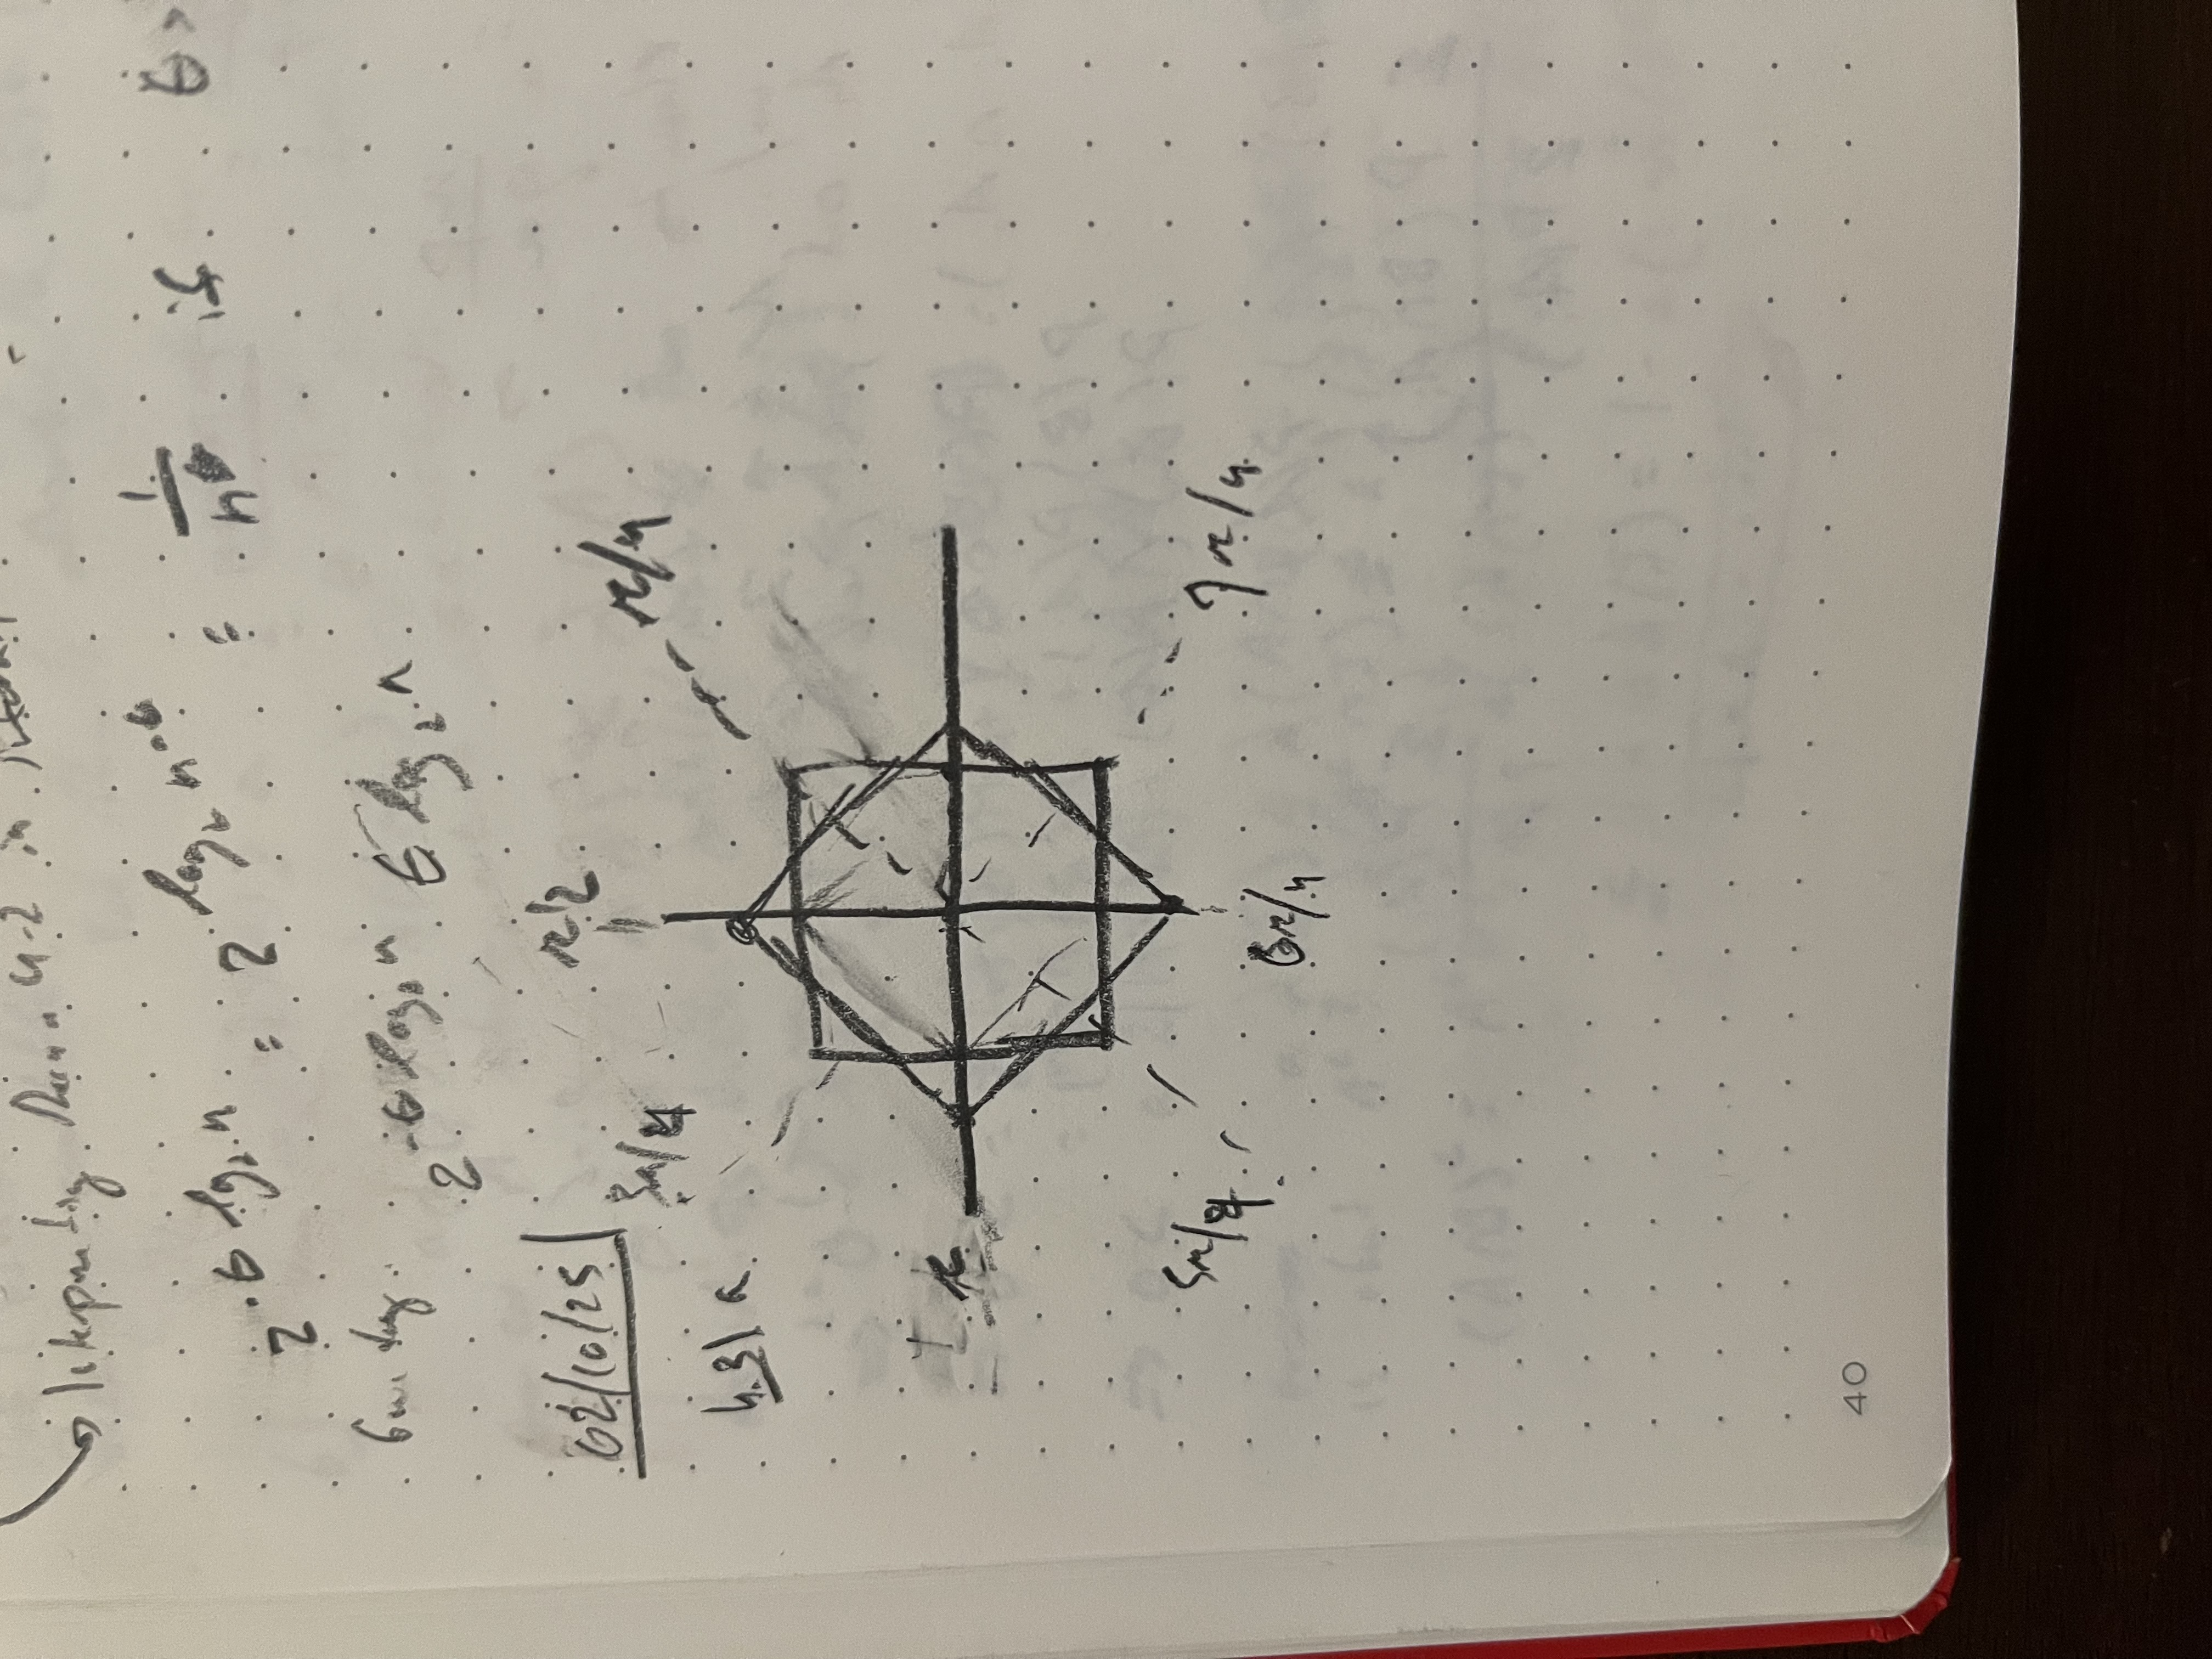
\includegraphics[angle=270, width=0.5\textwidth]{problem-4.3.a.jpg}
		\caption{Diagram for Question 4.3.a}
		\label{fig:example1}
	\end{figure} 
	\noindent Note that the $\limsup$ is the union of the two squares in the above picture, as any point that appears within one of the two squares will appear infinitely often. $\liminf$ is the intersection of the two squares - as only the points in the intersection will appear in every tail set.
	
	\item $\theta$ is rational. In this case:
	$$
		\text{angle}_n = 2\pi n * p/q = \frac{2p n\pi}{q}
	$$
	Note - we will have a picture like above, with cycle of $q$. Note that:
	$$
		A_{k} = A_{q + k} = A_{2q + k}
	$$
	For $k \in [q]$, as:
	$$
		\frac{2p (tq + k)\pi}{q} =
		2\pi pt + 2\pi \frac{pk}{q}
	$$
	Note that as $t$ and $p$ are integers, $2\pi pt$ is an integer multiple of $2\pi$, which just circles back to the angle of zero. And then, the added fraction of $ 2\pi \frac{pk}{q}$ is always the same. So, the union of the sets $A_k$ is the $\limsup$, like above, and the intersection is the $\liminf$, like above.
	
	\item $\theta$ is irrational. Note, in this case, we have that:
	$$
		\text{remainder } 2\pi n \theta / 2\pi
	$$
	Is dense in $[0,2\pi]$. Let's just assume that is the case for now. And so, take $x \not\in D$, where $D$ is the unit disk, but $x \in A_n$ for some $A_n$. Note, I think it might appear infinitely often in some $A_n$.
	\\\\
	Just making a leap here: but I think $\limsup A_n$ is the disk of radius $\sqrt{2}$, whereas $\liminf A_n$ is the disk of radius $1$. If you want to appear in every tail sequence - you have to be inside the unit disc.
		
\end{enumerate}

\subsubsection{4.7 Independence Complement Criteria} For events $A_1, \cdots, A_n$ consider the $2^n$ equations $P(B_1 \cap \cdots \cap B_n) = P(B_1) \cdots P(B_n)$ with $B_i = A_i$ or $B_i = A_i^c$ for each $i$. Show that $A_1, \cdots, A_n$ are independent if all these equations hold.
\\\\
We note a similar criteria that we have already approved - consider the $2^n$ equations $P(C_1 \cap \cdots \cap C_n) = P(C_1) \cdots P(C_n)$ with $C_i = A_i$ or $C_i = \Omega$ for each $i$. If each of these holds, then the $A_i$ are independent. We prove that if the $B$ equations hold, the $C$ equations holds. Thus, the $B$ equations also imply independence.
\\\\
First, assume one of the $C_i$ is $\Omega$. Thus, we have by countable additivity:
$$
	P(C_1 \cap \cdots \cap C_n) = 
	P(A_1 \cap \cdots \cap A_i \cap \cdots \cap A_n) + 
	P(A_1 \cap \cdots \cap A_i^c \cap \cdots \cap A_n)
$$
By the $B$ equations, the above equals:
$$
	= (P(A_i) + P(A_i)^c)(P(A_1) \cdots \widehat{P(A_i)} \cdots P(A_n)) =
	P(C_1) \cdots P(C_n)
$$
Now, we can take this result, and prove the equations hold for two $\Omega$ in the same way, and so on. Thus, we have that the $C_i$ equations hold if the $B_i$ equations hold, and the $B_i$ equations imply independence. Note, independence clearly implies the $B_i$ equations hold, so its an if and only if. qed.

\subsubsection{4.8 Class $\acal$ Partitions of $\Omega$} Recall that $\omega$ and $\omega'$ are called $\acal$ equivalent if, for every $A \in \acal$, $\omega$ and $\omega'$ lie either both in $A$ or both in $A^c$. That is:
$$
	I_A(\omega) = I_A(\omega') \quad\quad\quad A \in \acal
$$
This is clearly an equivalence relation, and this relation partitions $\Omega$. Note, there are $2^{|\acal|}$ possible equivalence classes - as for each $A \in \acal$, being in $A$ or $A^c$ defines two difference classes (note, this might not be entirely accurate if $\acal$ contains the complement or not. But, the idea is there). Also note - we proved that if $\omega$ and $\omega'$ are $\acal$ equivalent, then they are also $\sigma(\acal)$ equivalent.
\\\\
In this problem, we want to describe the $\acal$ partition for each of the following classes:
\begin{enumerate}
	\item The class of finite and cofinite sets. For this class - each $\omega$ would belong to a finite set of itself. And so, if $\omega' \neq \omega$, we would have $I_{\{\omega\}}(\omega) \neq I_{\{\omega\}}(\omega')$. The partition would be all singletons.
	
	\item The class of countable and cocountable sets. For this class - I again believe the partition would be the singletons. Say $\omega, \omega'$ both belong to a countable set $A$. Then, we have that $A - \{\omega'\}$ is also a countable set. In which case, $\omega$ and $\omega'$ are not in the same equivalence class.
	
	\item A partition (or arbitrary cardinality) of $\Omega$. So, each $A \in \acal$ is disjoint from the rest. We have that the $\omega \in A$ form an equivalence class - as $\omega,\omega' \in A$ also implies $\omega,\omega' \not\in B \in \acal$ for $B \neq A$.
	
	\item The level sets of $\sin(x)$, where $\Omega = \R$. Again, I believe this would form a partition of $\Omega$, as $\sin(x) = c$ has multiple $x$ that satisfy that value. If we want to describe the partitions - we have for $c \in [-1,1]$, the level set $L$ is:
	$$
		L = \{x \in \R : x = \arcsin(c) + 2n\pi \text{ or } x = \pi - \arcsin(c) + 2n\pi, n \in \Z\}
	$$
	Think of this in terms of the unit circle - $\arcsin(c)$ gives the $x$ value (angle value) on the positive $x$ axis. The $x$ value on the negative $x$ axis is symmetrical, or mirrored, which is given by $\pi - x$. This gives the set above.
	
	\item The $\sigma$ field in problem 3.5. In problem 3.5, we have $\Omega = \left\{(x,y) : 0 < x,y \leq 1\right\}$ is the unit square, and $\fcal$ is the class of sets of the form:
	$$
		\left\{(x,y) : x \in A, 0 < y \leq 1\right\}
	$$
	And let $P$ have value $\lambda(A)$ on this set. In the problem, we show that $(\Omega,\fcal,P)$ is a probability space. First, we note that $\fcal$ is a $\sigma$ algebra - as countable unions and intersections on the $x$ axis still remain within $\bcal$, and we still have all the ``height" from zero to one. We also clearly have $\Omega$ and complements. Probability measure still holds, as we still have countable additivity (if the $A$ are disjoint in $\bcal$, so are the corresponding sets above). It is also clear that for $A = \{(x,y) : 0 < x \leq 1, y = 1/2\}$, we have the outer measure $P^*(A) = 1$ while the inner measure $P^*(A) = 0$. That is essentially answering question 3.5.
	\\\\
	Now, we note that the $\acal$ partition of $\Omega$ is just straight lines $\{(x,y) : x \in (0,1], 0 < y \leq 1\}$. Every $\omega$ along such a line belongs to the same $A$ or $A^c$ for $A \in \fcal$ - this is because, each $A \in \fcal$ either contains the entire line, or it doesn't. Also, note that if $\omega$ and $\omega'$ are not on the same line - the singleton $\{x\}$ and $\{x'\}$ sets are within $\bcal$, so $\omega \in \{(x,y): 0 < y \leq 1\}$, but $\omega' \not\in \{(x,y): 0 < y \leq 1\}$. qed.
\end{enumerate}

\subsubsection{4.10 Independence does not imply Independent Information} Where by information, we mean which \textit{partition} of $\omega$ was selected. Note, some classes can be independent, but the information one class gives (ie, the partition that $\omega$ belongs to) might tell us which set in the other class the $\omega$ belongs to. This question essentially just emphasizes that the information notion is not altogether perfect.
\\\\
There is in the unit interval a set $H$ that is nonmeasurable in the extreme sense that its inner and outer Lebesgue measures are $0$ and $1$: $\lambda_*(H) = 0$ and $\lambda^*(H) = 1$. See problem 12.4 for its construction.
\\\\
\textbf{1.} Let $\Omega = (0,1]$, let $\gcal$ consist of the Borel sets in $\Omega$, and let $H$ be the set just described. Show that the class $\fcal$ of sets of the form $(H \cap G_1) \cup (H^c \cap G_2)$ for $G_1,G_2 \in \gcal$ is a $\sigma$ field, and that:
$$
	P\left[(H \cap G_1) \cup (H^c \cap G_2)\right] = \frac{1}{2}\lambda(G_1) + \frac{1}{2}\lambda(G_2)
$$
consistently defines a probability measure on $\fcal$. First, we show it is a $\sigma$ field. Clearly, it contains complements, as:
$$
	\left[(H \cap G_1) \cup (H^c \cap G_2)\right]^c =
	(H \cap G_1^c) \cup (H^c \cap G_2^c)
$$
Note $x \in (H \cap G_1^c) \implies x \not\in (H \cap G_1) \land x \not\in (H^c \cap G_2)$. Similar can be shown for $x \in (H^c \cap G_2^c)$, and so:
$$
	(H \cap G_1^c) \cup (H^c \cap G_2^c) \subseteq (H \cap G_1) \cup (H^c \cap G_2)
$$ 
Now, take $x \in \left[(H \cap G_1) \cup (H^c \cap G_2)\right]^c$. This implies $x \in H^c \lor x \in G_1^c$ \textit{and} $x \in H \lor x \in G_2^c$. If $x \in H^c$, then $x \not\in H$, in which case $x \in G_2^c$, and we have $x \in (H \cap G_2^c$. Similar for $x \in H$. Final case is $x \in G_1^c$ and $x \in G_2^c$, in which case $x \in H$ or $x \in H^c$. In all cases:
$$
	\left[(H \cap G_1) \cup (H^c \cap G_2)\right]^c \subseteq
	(H \cap G_1^c) \cup (H^c \cap G_2^c) 
$$
$$
	\implies
	\left[(H \cap G_1) \cup (H^c \cap G_2)\right]^c =
	(H \cap G_1^c) \cup (H^c \cap G_2^c)
$$
Note, see problem 2.7 for closed under countable unions (it is actually easier than the above. So yes, $\fcal$ is a $\sigma$ field. Now, we want to show that:
$$
	P\left[(H \cap G_1) \cup (H^c \cap G_2)\right] = \frac{1}{2}\lambda(G_1) + \frac{1}{2}\lambda(G_2)
$$
consistently defines a probability measure on $\fcal$. I will show that:
$$
	\lambda(G_1) = \lambda^*(G_1) = \lambda^*(H \cap G_1)
$$
First, by monotonicity of the outer measure, we have:
$$
	\lambda^*(H \cap G_1) \leq \lambda^*(G_1) \quad\quad\text{and}\quad\quad
	\lambda^*(H \cap G_1^c) \leq \lambda^*(G_1^c) = 1 - \lambda^*(G_1)
$$
Now, we note that as $G_1 \in \gcal = \bcal$, $G_1$ is measurable, and so:
$$
	\lambda^*(H \cap G_1) + \lambda^*(H \cap G_1^c) = \lambda^*(H) = 1 \implies
	\lambda^*(H \cap G_1) + 1 - \lambda^*(G_1) \geq 1
$$
$$
	\implies \lambda^*(H \cap G_1) \geq \lambda^*(G_1)
$$
Thus, we indeed have:
$$
	\lambda^*(H \cap G_1) = \lambda^*(G_1)
$$
We can similarly show:
$$
	\lambda^*(H \cap G_3) = \lambda^*(G_3)
$$
Given that $H \cap G_1 = H \cap G_3$, we thus must have:
$$
	\lambda(G_1) = \lambda(G_3)
$$
And similarly, we have $\lambda(G_2) = \lambda(G_4)$. Thus, we can conclude that:
$$
	(H \cap G_1) \cup (H^c \cap G_2) = (H \cap G_3) \cup (H^c \cap G_4) \implies
	\lambda(G_1) + \lambda(G_2) = \lambda(G_3) + \lambda(G_4)
$$
And the probability measure is consistent. Now, we note it is a probability measure, as it is clearly between $0$ and $1$, $P(\Omega) = 1$, and we have countable additivity (disjoint unions, transfer the disjoint unions into the $H \cap$ and $H^c \cap$ terms, and then rely on countable additivity of $\lambda$).
\\\\
\textbf{2.} Show that $P(H) = 1/2$ and that $P(G) = \lambda(G)$ for $G \in \gcal$. First, note that:
$$
	P(H) = P\left[(H \cap \Omega) \cup (H^c \cap \emptyset)\right] =
	1/2\lambda(\Omega) + 1/2\lambda(\emptyset) = 1/2
$$
Now, note that:
$$
	P(G) = P\left[(H \cap G) \cup (H^c \cap G)\right] =
	1/2\lambda(G) + 1/2\lambda(G) = \lambda(G)
$$
\textbf{3.} Show that $\gcal$ is generated by a countable subclass. Note, in problem 2.11, we showed that with the rational intervals, and that it contained the singletons.
\\\\
\textbf{4.} Show that $\gcal$ contains all the singletons and that $H$ and $\gcal$ are independent (in the sense that $\gcal$ is a class contained within $\fcal$). Above, we noted that $\gcal$ contains the singletons. Independence follows if for $G \in \gcal$, we have:
$$
	P(H \cap G) = P(H)P(G) = 1/2\lambda(G)
$$
Where the last equality is by part 3. Note that:
$$
	P(H \cap G) = P\left[(H \cap G) \cup (H^c \cap \emptyset)\right] = 1/2\lambda(G) + 1/2* 0 = 1/2\lambda(G)
$$
Thus, $H$ and $\gcal$ are independent.
\\\\
This construction proves the following: There exists a probability space $(\Omega, \fcal, P)$, a $\sigma$ field $\gcal$ in $\fcal$, and a set $H \in \fcal$, such that $P(H) = 1/2$, $H$ and $\gcal$ are independent, and $\gcal$ is generated by a countable subclass and contains all the singletons.
\\\\
This relates to example 4.10, in which, even though $\gcal$ and $H$ are independent, the ``information" contained in $G$ would tell us whether or not the drawn $\omega$ is in $H$ or not. However, note that with this example - the $\gcal$ is more \textit{natural} - it is countably generated, and contains singletons. In fact - it is the borel sets! However, the example involves the pathological set $H$, which throws everything for a loop.

\subsubsection{4.11 Different Criteria for $P(\limsup_n A_n) = 1$}
\begin{enumerate}
	\item If $A_1, A_2, \cdots$ are independent events, then prove:
	$$
		P\left(\bigcap_{n=1}^\infty A_n\right) = \prod_{n=1}^\infty P(A_n)
	$$
	And:
	$$
		P\left(\bigcup_{n=1}^\infty A_n\right) = 1 - \prod_{n=1}^\infty (1 - P(A_n))
	$$
	From these facts, derive the second Borel-Cantelli lemma by the well-known relation between infinite series and products (I would guess, it is the exponential fact).
	\\\\
	We note that for a finite sequence, independence implies:
	$$
		P\left(\bigcap_{n=1}^k A_n\right) = \prod_{n=1}^k P(A_n)
	$$
	We note that by continuity from above, we have:
	$$
		P\left(\bigcap_{n=1}^\infty A_n\right) = \prod_{n=1}^\infty P(A_n)
	$$
	We have by De'Morgan's laws, and independence implying independence of complements:
	$$
		P\left(\bigcup_{n=1}^\infty A_n\right) = 1 - P\left(\bigcap_{n=1}^\infty A_n^c\right) =
		1 - \prod_{n=1}^\infty (1 - P(A_n))
	$$
	Recall, the Borel Cantelli Lemma states that if $\{A_n\}$ is an independent sequence of events, and $\sum_n P(A_n)$ diverges, then $P(\limsup_n A_n) = 1$. Note, this follows if the complement of the $\limsup$ equals $0$, which follows if $\bigcap_{k=n}^\infty A_k^c = 0$ for all $n$. Note, we have $A_k^c$ are independent by above, and so:
	$$
		P\left(\bigcap_{k=n}^\infty A_k^c\right) = \prod_{k=n}^\infty (1 - P(A_k)) \leq
		\exp\left[-\sum_{k=n}^\infty P(A_k)\right] = 0
	$$
	As we know the sum diverges, and for $x \in [0,1]$, $(1-x) \leq \exp(-x)$. Note - the above is essentially just the proof for the second lemma, but made easier, as we don't have to apply a limit argument in the middle of the above steps, by the facts above. If we wanted to just \textit{derive} the lemma, then we might use the \href{https://en.wikipedia.org/wiki/Weierstrass_product_inequality?utm_source=chatgpt.com}{Weierstrass product inequality}. We have:
	$$
		1 - \sum_{n=1}^\infty P(A_n) \leq \prod_{n=1}^\infty (1 - P(A_n)) \leq \exp\left[-\sum_{n=1}^\infty P(A_n)\right]
	$$
	From this, we have:
	$$
		P\left(\bigcup_{n=1}^\infty A_n\right) = 1 - \prod_{n=1}^\infty (1 - P(A_n)) \geq
		1 - \exp\left[-\sum_{n=1}^\infty P(A_n)\right] = 1
	$$
	So, the probability of each union of $A_n$, and each tail sequence union of $A_n$, is $1$. Note, from this, we can derive $P(\limsup_n A_n) = 1$, as it is an intersection of unions of probability one. Note, that by itself isn't enough, but we can use continuity from above to prove it equals $1$ as well (as the unions each contain each other). qed.
	
	\item Show that $P(\limsup_n A_n) = 1$ if for each $k$ the series $\sum_{n > k} P(A_n | A_k^c \cap \cdots \cap A_{n-1}^c)$ diverges. From this deduce the second Borel-Cantelli lemma once again.
	\\\\
	Just from an informal ``information" level - the independent parts of each $A_n$, the probability of each $A_n$ when you are given the rest of the previous $A_k$ - diverges (note, I treat knowing $A_k^c$ equivalent to knowing $A_k$).
	\\\\
	Recall, we have:
	$$
		\limsup_n A_n = \bigcap_{n=1}^\infty \bigcup_{k=n}^\infty A_k
	$$
	As noted above, we can prove this probability equals one if each $\bigcup_{k=n}^\infty A_k$ equals one. Note - I think we can use the ratio test. If the limit of the ratios exists - then it must be greater than or equal to 1, as a ratio less than 1 would imply convergence. For the ratio test, we would have ratios of:
	$$
		\frac{P(A_k^c \cap \cdots \cap A_n^c \cap A_{n+1})}{P(A_k^c \cap \cdots \cap A_n^c)}
		\frac{P(A_k^c \cap \cdots \cap A_{n-1}^c)}{P(A_k^c \cap \cdots \cap A_{n-1}^c \cap A_n)}
	$$
	$$
		=
		\frac{P(A_k^c \cap \cdots \cap A_n^c \cap A_{n+1})}{P(A_k^c \cap \cdots \cap A_n^c)}
		\frac{P(A_k^c \cap \cdots \cap A_{n-1}^c \cap A_n^c) + P(A_k^c \cap \cdots \cap A_{n-1}^c \cap A_n)}{P(A_k^c \cap \cdots \cap A_{n-1}^c \cap A_n)}
	$$
	$$
		=
		\frac{P(A_k^c \cap \cdots \cap A_n^c \cap A_{n+1})}{P(A_k^c \cap \cdots \cap A_n^c)}
		\left(
		\frac{P(A_k^c \cap \cdots \cap A_{n-1}^c \cap A_n^c)}{P(A_k^c \cap \cdots \cap A_{n-1}^c \cap A_n)} + 1
		\right)
	$$
	I'm not sure if these ratios will actually help us.
	\\\\
	We will first derive the second Borel-Cantelli lemma, just to get something on the board. Assume that the $A_n$ are independent, and their sum diverges. Then, we have:
	$$
		\sum_{n > k} P(A_n | A_k^c \cap \cdots \cap A_{n-1}^c) = 
		\sum_{n > k} \frac{P(A_n \cap A_k^c \cap \cdots \cap A_{n-1}^c)}{P(A_k^c \cap \cdots \cap A_{n-1}^c)}
	$$
	$$
		=
		\sum_{n > k} \frac{P(A_n) P(A_k^c) \cdots P(A_{n-1}^c)}{P(A_k^c) \cdots P(A_{n-1}^c)} =
		\sum_{n > k} P(A_n) = \infty
	$$
	Where the $= \infty$ comes from every tail sequence diverging as well. Thus, we have that $P(\limsup_n A_n) = 1$, and this tail series fact is actually stronger. Now, we note, that $P(\limsup_n A_n) = 1$ if we have for every $k$:
	$$
		P\left[\bigcap_{n \geq k} A_n^c\right] = 0
	$$
	We use this fact in the original proof. Assume by contradiction that we have at least one $k$ such that the above is greater than $0$. Then, we note by assumption:
	$$
		\sum_{n > k} P(A_n | A_k^c \cap \cdots \cap A_{n-1}^c) = \infty
	$$
	$$
		\implies
		\sum_{n > k} P(A_n \cap A_k^c \cap \cdots \cap A_{n-1}^c) \frac{1}{P(A_k^c \cap \cdots \cap A_{n-1}^c)} = \infty
	$$
	Now, by contradiction, we have assumed:
	$$
		P\left[\bigcap_{n \geq k} A_n^c\right] = \epsilon > 0 \implies
		P(A_k^c \cap \cdots \cap A_{n-1}^c) \downarrow \epsilon
	$$
	Note, this implies the fraction approaches some constant $1/\epsilon$, and we can pull it out to conclude the first series diverges. More rigorously, for some $N$ large enough, for $n \geq N$, we have that:
	$$
		\epsilon \leq P(A_k^c \cap \cdots \cap A_{n-1}^c) \leq 2\epsilon
	$$
	Thus, on the tail, we find:
	$$
		\infty = \sum_{n > N} P(A_n \cap A_k^c \cap \cdots \cap A_{n-1}^c) \frac{1}{P(A_k^c \cap \cdots \cap A_{n-1}^c)} \geq
		2\epsilon \sum_{n > N} P(A_n \cap A_k^c \cap \cdots \cap A_{n-1}^c)
	$$
	$$
		\implies \sum_{n > k} P(A_n \cap A_k^c \cap \cdots \cap A_{n-1}^c) = \infty
	$$
	This is a contradiction, as we have each of the sets in the above sum are disjoint, and so their sum cannot be more than one. Thus, we must conclude for all $k$:
	$$
		P\left[\bigcap_{n \geq k} A_n^c\right] = 0 \implies
		P(\limsup_n A_n) = 1
	$$
	Note: I used help online to solve this. My problem was - I was too focused on directly proving it. I had gotten to the intersections equal 0/unions equal one statement - but direct proof was the problem. I think if I had pivoted quicker, I could have solved this one.
	
	\item Show by example that $P(\limsup_n A_n) = 1$ does not follow from the divergence of $\sum_n P(A_n | A_1^c \cap \cdots \cap A_{n-1}^c)$ alone.
	\\\\
	Thinking in terms of ``information" - I think this might follow if $A_1$ is a really \textit{small} event. Then, knowing $A_1^c$ might mean that you know \textit{a lot}, in which case the probabilities in the sum are large.
	\\\\
	Can't really figure this one out. First, we need $A_n$ to not be disjoint from the $A_k^c$ for $k < n$, as otherwise our conditional probabilities will be $0$. Then, we need $A_1^c$ to be restrictive enough so that the fraction becomes something like $x/x$, which is close to $1$. 
	
	\item Show that $P(\limsup_n A_n) = 1$ if and only if $\sum_n P(A \cup A_n)$ diverges for each $A$ of positive probability.
	\\\\
	Assume that $P(\limsup_n A_n) = 1$ and take $A$ such that $P(A) > 0$. Note, we have that:
	$$
		B_k = \bigcup_{i = k}^\infty A_i \implies 1 = P(\limsup_n A_n) =
		P\left(\bigcap_{n=1}^\infty B_n\right) \leq
		P(B_k)
	$$
	$$
		\implies P(B_k) = 1
	$$
	Assume by contradiction that $\sum_n P(A \cup A_n)$ converges. Then, for some $k$ large enough, we have for $\epsilon < P(A)$:
	$$
		P(A \cap B_k) = P\left(A \cap \bigcup_{i = k}^\infty A_i\right) =
		P\left(\bigcup_{i = k}^\infty A \cap A_i\right) \leq
		\sum_{i = k}^\infty P(A \cap A_i) < \epsilon 
	$$
	However, we note:
	$$
		P(A) = P((A \cap B_k) \cup (A \cap B_k^c)) = P(A \cap B_k) + P(A \cap B_k^c) = P(A \cap B_k)
	$$
	As $P(A \cap B_k^c) \leq P(B_k^c) = 0$. Thus, we have a contradiction, as we have found:
	$$
		P(A) = P(A \cap B_k) < \epsilon < P(A)
	$$
	And so, by contradiction, we have that $\sum_n P(A \cup A_n)$ diverges. Now, we go the other direction, and assume that the sum diverges for all $A$ with positive probability. We have $P(\limsup_n A_n) = 1$ if and only if $P(B_k) = 1$. By contradiction, assume that $P(B_k) < 1$, in which case $P(B_k) > 1$. Then, we have:
	$$
		\sum_{i=k}^\infty P(B_k^c \cap A_i) \text{ diverges} \implies
		\sum_{i=k}^\infty P(A_i - B_k) \text{ diverges}
	$$
	$$
		\implies
		\sum_{i=k}^\infty P(A_i - (A_k \cup \cdots \cup A_{i-1})) \text{ diverges}
	$$
	Note, the last step is because $A_k \cup \cdots \cup A_{i-1} \subseteq B_k$. Now, note that the above is a summation of disjoint sets, and so, we have:
	$$
		\implies
		P\left(\bigcup_{i=k}^\infty A_i - (A_k \cup \cdots \cup A_{i-1})\right) = \infty
		\implies
		P(B_k) = \infty
	$$
	This is a contradiction, as an event must have less than or equal to $1$ probability. And so, by contradiction, we have that $P(B_k) = 1$ and thus $P(\limsup_n A_n) = 1$. qed.
	
	\item If sets $A_n$ are independent and $P(A_n) < 1$ for all $n$, then $P(A_n \io) = 1$ if and only if $P(\bigcup_n A_n) = 1$.
	\\\\
	We first go in the easy direction. Note, $P(A_n \io) = 1$ if and only if $P(B_k) = 1$ for all $k$. Note, for $k = 1$, we have:
	$$
		1 = P(B_1) = P\left(\bigcup_n A_n\right)
	$$
	And so now, we go in the other direction. Recall, one sufficient condition for $P(A_n \io) = 1$ is that:
	$$
		P\left(\bigcap_{i=k} A_i^c\right) = 0
	$$
	For all $i$. Note, we have by assumption:
	$$
		P\left(\bigcap_{i=1} A_i^c\right) = 0
	$$
	As the $A_i^c$ are independent events as well, by part $a$, we have:
	$$
		P\left(\bigcap_{i=k} A_i^c\right) = \prod_{i=k}^\infty P(A_i^c)
	$$
	For $j = 1, \cdots, k-1$, we note that $P(A_j) < 1$, and so we have that $P(A_j^c) > 0$. And so, we have that:
	$$
		0 = P\left(\bigcap_{i=1} A_i^c\right) =
		\lim_{n \to \infty} \prod_{i=1}^n P(A_i^c) =
		P(A_1^c) \cdots P(A_{k-1}^c) \lim_{n \to \infty} \prod_{i=k}^n P(A_i^c)
	$$
	$$
		\implies
		0 = P(A_1^c) \cdots P(A_{k-1}^c) P\left(\bigcap_{i=k} A_i^c\right)
	$$
	As $P(A_1^c) \cdots P(A_{k-1}^c) > 0$, we must have for all $k$:
	$$
		0 = P\left(\bigcap_{i=k} A_i^c\right) \implies P(A_n \io) = 1
	$$
	Thus, we can indeed conclude that if sets $A_n$ are independent and $P(A_n) < 1$ for all $n$, then $P(A_n \io) = 1$ if and only if $P(\cup_n A_n) = 1$. qed.
\end{enumerate}

\subsubsection{4.14 Infinite Independent Events Criteria for a Nonatomic Space} Suppose that there are in $(\Omega, \fcal, P)$ independent events $A_1, A_2, \cdots$ such that, if:
$$
	\alpha_n = \min\left\{P(A_n), 1 - P(A_n)\right\}
$$
Then $\sum \alpha_n = \infty$. Show that $P$ is \textit{nonatomic}. 
\\\\
Recall - nonatomic means that if $P(A) > 0$, there exists a $B$ such that $B \subset A$ and $0 < P(B) < P(A)$, and $A,B \in \fcal$. Note, in problem 2-19, we prove that $\bcal$ is nonatomic with the lebesgue measure (deriving a contradiction from a single point needing to have $0$ lebesgue measure). We also showed that in the nonatomic case, that for $0 \leq x \leq P(A)$, there exists a $B$ such that $B \subset A$ and $P(B) = x$. Finally, we proved that if $p_1, p_2, \cdots$ are nonnegative and add to $1$, then $A$ can be decomposed into sets $B_1, B_2, \cdots$ such that $P(B_n) = p_nP(A)$.
\\\\
Take an $A \in \fcal$. We just have to show that there is a $B$ such that $B \subset A$, and $0 < P(B) < P(A)$ and $B \in \fcal$. Take $B_i$ as either $A_i$ or $A_i^c$, whichever satisfies $P(B_i) = \alpha_i$. Note, by Borel-Cantelli, we have $P(B_i \io) = 1$, and by 4.11e, we have:
$$
	P(\cup_i B_i) = 1
$$
Examine each $A \cap B_i$. We note for some $B_i$, we have that $0 < P(A \cap B_i) < P(A)$, and thus $(\Omega,\fcal,P)$ is nonatomic. First, note they all can't be zero, as that would imply:
$$
	0 = P(A \cap B_i) \implies
	0 = P(\cup A \cap B_i) = P(A \cap \cup B_i) = P(A)
$$
Which is a contradiction. Note, the only thing to do now is prove that if $P(A \cap B_i) > 0$, we don't have $P(A \cap B_i) = P(A)$. However, this could be the case - what if the $B_i$ are disjoint, and $A = B_j$. This path will not work.
\\\\
\textbf{Attempt 2} Using the solution at the back of the book. First, note that:
$$
	\lim_{n \to \infty} \max P(B_1 \cap \cdots \cap B_n) = 0
$$
Here, we take $B_i$ as either $A_i$ or $A_i^c$ - note, we have:
$$
	P(B_1 \cap \cdots \cap B_n) = \prod_{i=1}^n P(B_i) \leq \exp\left(-\sum_{i=1}^n P(B_i)\right)
$$
Note, no matter the sum, it always diverges, and so yes, the limit is indeed $0$, even if you take the maximizing $B_i$. Now, define:
$$
	C_x = \left[\omega: \sum_n I_{A_n}(\omega) 2^{-n} \leq x\right]
$$
First note, $C_x$ contains all $\omega$ not in the $A_n$. Then, it would pick up the $\omega$ that appear sporadically, or in tail sequences far away enough such that the sum of the corresponding $2^{-n}$ does not exceed $x$. We want to show that:
$$
	P(A \cap C_x)
$$
Is continuous in $x$. Note that the above is maximized for $x = 1$, in which case $P(A \cap C_1) = P(A)$, as $C_1 = \Omega$, and minimized for $x = 0$, in which case $P(A \cap C_0) = P\left(A \cap \left(\cup A_i\right)^c\right) = 0$, as we have $P(\cup A_i) = 1$, and so its complement has probability zero. We want to show it is continuous in $x$. So, take some $c \in (0,1)$. We want to show that as $x_n \to c$, we have:
$$
	\lim_n P(A \cap C_{x_n}) = P(A \cap C_c)
$$
I believe this can be done by looking at the symmetric difference:
$$
	(A \cap C_{x_n}) \triangle (A \cap C_c)
$$
And noting that for $x_n$ close enough to $c$, the $\omega$ in one of the sets but not the other must be contained within small enough dyadic intervals. Or, we can make use of the fact that the maximum goes to $0$. We first assume that $x_n \uparrow c$. Later, we will generalize the argument for all $x_n \to c$. Note, in this case, we have:
$$
	A \cap C_{x_n} \subseteq A \cap C_c \implies
	P(A \cap C_c) - P(A \cap C_{x_n}) = 
	P(A \cap C_c - A \cap C_{x_n})
$$
$$
	= P(A \cap (C_c - C_{x_n})) \leq
	P(C_c - C_{x_n})
$$
So, we examine:
$$
	\omega \in C_c - C_{x_n}
$$
Note, $x_n$ can be arbitrarily close to $c$, and so $\omega \in C_c - C_{x_n}$ implies:
$$
	c - \epsilon \leq \sum_n I_{A_n}(\omega)2^{-n} \leq c
$$
Note, $c$ has at most two dyadic expansions (terminating and non-terminating):
$$
	c = \sum_n d^1_n(c)2^{-n} =
	\sum_n d^2_n(c)2^{-n}
$$
If $\epsilon < 2^{-k}$, we have that $\omega$ must satisfy for $n = 1, \cdots, k-1$:
$$
	\forall n \,\,\, I_{A_n}(\omega) = d^1_n(c) \text{ or } \forall n \,\,\, I_{A_n}(\omega) = d^2_n(c)
$$
If $\omega$ doesn't satisfy either of the two above equations, then the difference:
$$
	\left|\sum_n d^i_n(c)2^{-n} - \sum_n I_{A_n}(\omega)2^{-n}\right| > 2^{-k} > \epsilon
$$
Note, by the fact that for any \textit{specific} choice of $B_i$, we have:
$$
	\lim_{n \to \infty} \max P(B_1 \cap \cdots \cap B_n) = 0
$$
We thus have that:
$$
	\lim_{n \to \infty} P(C_c - C_{x_n}) \leq
	\lim_{n \to \infty} P(B^1_1 \cap \cdots \cap B^1_n) + P(B^2_1 \cap \cdots \cap B^2_n) = 0
$$
And so, for $x_n \uparrow c$, we indeed have:
$$
	\lim_n |P(A \cap C_c) - P(A \cap C_{x_n})| = \lim_n P(A \cap C_c) - P(A \cap C_{x_n}) \leq \lim_{n \to \infty} P(C_c - C_{x_n}) \leq 0
$$
$$
	\implies \lim_n P(A \cap C_{x_n}) = P(A \cap C_c)
$$
Now, for $x_n \to c$. Note, we can still prove that:
$$
	\lim_n |P(A \cap C_c) - P(A \cap C_{x_n})| = 0
$$
As either $A \cap C_c \subseteq A \cap C_{x_n}$, or vice versa, and we can still apply the argument for the bigger interval $(c-\epsilon,c+\epsilon)$ to conclude that the $\omega \in (A \cap C_{x_n}) \triangle (A \cap C_c)$ have to be in one of two specific sequences of $B_i$, which both have probability $0$. Thus, we indeed have that:
$$
	P(A \cap C_x)
$$
Is continuous in $x$. Thus, we can conclude there is some $x$ such that:
$$
	0 < P(A \cap C_x) < P(A)
$$
We clearly have $A \cap C_x \subseteq P(A)$. So, the final thing to note is that $A \cap C_x \in \fcal$, which comes from $C_x \in \fcal$. Note, the function describing $C_x$ can be shown to be a measurable mapping, in which case the preimage of an interval $[0,x]$ would be a measurable set as well. Note, clearly each partial sum is a measurable mapping (as the preimage is clearly measurable), and thus the infinite sum is measurable as well. This actually gives us a way to directly prove $C_x$ is measurable. First, note that for:
$$
	C^k_x = \left[\omega: \sum_{n=1}^k I_{A_n}(\omega) 2^{-n} \leq x\right]
$$
We have that $C^k_x$ is clearly measurable. There are certain sequences of $x \in B_1 \cap \cdots \cap B_k$, where $B_i = A_i$ or $A_i^c$, that satisfy the above equation. One such example is $x \in A_1^c \cap \cdots \cap A_k^c$. So, $C^k_x \in \fcal$, as $C^k_x$ is a finite union of finite intersections of measurable $B_i$. Now, we have that:
$$
	C_x = \bigcap_{k=1}^\infty C^k_x
$$
Clearly, $\omega \in C^k_x \implies \omega \in C_x$, as we can just take $\omega \in A_i^c$ for $i > k$. Now, take $\omega \in C_x$. We note that $\omega$ must be in $B_1, \cdots, B_k$ such that the sum satisfies:
$$
	\sum_{n=1}^k I_{A_n}(\omega) 2^{-n} \leq x
$$
Given that the infinite sum also satisfies being less than $x$. And so, $\omega \in C_x \implies \omega \in C^k_x$ for all $k$. Thus, we have that $C_x$ is a countable intersection of $\fcal$ sets, and so $C_x$ is within $\fcal$.
\\\\
Thus, we have proved that if there are in $(\Omega, \fcal, P)$ independent events $A_1, A_2, \cdots$ such that for:
$$
	\alpha_n = \min\left\{P(A_n), 1 - P(A_n)\right\}
$$
Then $\sum \alpha_n = \infty$, we have that $P$ is \textit{nonatomic}. qed.

\subsubsection{4.15 Density of the Square-Free Integers} Let $F$ be the set of square-free integers - those integers not divisible by any perfect square. Let $F_l$ be the set of $m$ such that $p^2|m$ ($p^2$ divides $m$) for no $p \leq l$, and show that $D(F_l) = \prod_{p \leq l}(1-p^{-2})$. Show that $P_n(F_l - F) \leq \sum_{p > l} p^{-2}$, and conclude that the square-free integers have density:
$$
	\prod_p (1-p^{-2}) = 6/\pi^2
$$
We need to recall a lot of the above notation. Its all from problem 2.18. We have that:
$$
	P_n(A) = \frac{1}{n}\#\left\{m : 1 \leq m \leq n, m \in A\right\}
$$
We also have that $P_n$ is a \textit{discrete} probability measure on $\Omega = \{1, 2, \cdots\}$. We define the \textit{density} as:
$$
	D(A) = \lim_n P_n(A)
$$
We first want to show:
$$
	D(F_l) = \prod_{p \leq l}(1-p^{-2})
$$
Note - I will first go with the assumption that $p$ is \textit{prime}. Note, assuming prime makes things easier, as we have that $lcm(p_1,p_2) = p_1p_2$, and we similarly have $lcm(p_1^2,p_2^2) = p_1^2p_2^2$. Further, in problem 2.18 (which this problem seems to be a continuation of), $p$ referred to prime numbers as well.
\\\\
We recall the notation that $M_a = \{ak: k = 1, 2, \cdots\}$. These are periodic sets, and in problem 2.18, we proved the following (note, it should also be intuitively clear):
$$
	P_n(M_a) = \frac{1}{n}\floor{\frac{n}{a}} \to \frac{1}{a} = D(M_a)
	\quad\quad\quad
	M_a \cap M_b = M_{lcm(a,b)}
$$
We clearly have:
$$
	F_l = \left[\bigcup_{p \leq l} M_{p^2}\right]^c \implies
	F_l = \bigcap_{p \leq l} M_{p^2}^c
$$
We now note that for prime $p_1, \cdots, p_k$, we have that:
$$
	P_n\left[M_{p_1^2} \cap \cdots \cap M_{p_k^2}\right] =
	P_n\left[M_{lcm(p_1^2, \cdots, p_k^2)}\right] =
	P_n\left[M_{p_1^2 \cdots p_k^2}\right] =
	\frac{1}{n}\floor{\frac{n}{p_1^2 \cdots p_k^2}} \to 
	\frac{1}{p_1^2 \cdots p_k^2}
$$
So, we now find:
$$
	D(F_l) = 
	\lim_{n \to \infty} P_n(F_l) =
	1 - \lim_{n \to \infty} P_n\left(\bigcup_{p \leq l} M_{p^2}\right)
$$
We now make use of the inclusion-exclusion principle to find the above equals:
$$
	1 - 
	\lim_{n \to \infty} \sum_{1 < p_1 \leq l} P_n\left(M_{lcm(p_1^2)}\right) +
	\lim_{n \to \infty} \sum_{1 < p_1 < p_2 \leq l} P_n\left(M_{lcm(p_1^2,p_2^2)}\right) + \cdots
$$
$$
	+ (-1)^k \lim_{n \to \infty} \sum_{1 < p_1 < p_2 < \cdots < p_k \leq l} 
	P_n\left(M_{lcm(p_1^2,p_2^2, \cdots, p_k^2)}\right)
$$
$$
	=
	1 -
	\sum_{1 < p_1 \leq l} \frac{1}{p_1^2} +
	\sum_{1 < p_1 < p_2 \leq l} \frac{1}{p_1^2p_2^2} + \cdots +
	(-1)^k \sum_{1 < p_1 < p_2 < \cdots < p_k \leq l} \frac{1}{p_1^2 \cdots p_k^2}
$$
$$
	= (1-p_1^2)(1-p_2^2) \cdots (1-p_k^2)
$$
Where the final equality is a well known formula for the multiplication of $(1-p_i)$ terms. (also called the inclusion-exclusion principle). The second inequality is making use of our limit fact proved above. Thus, we indeed have:
$$
	D(F_l) = \prod_{p \leq l}(1 - p^{-2})
$$
Now, the task is to show that $P_n(F_l - F) \leq \sum_{p > l} p^{-2}$. We note that:
$$
	F_l - F \subseteq \bigcup_{p > l} M_{p^2}
$$
Take $x \in F_l - F$. We have that $x$ is \textit{not} divisible by $p^2$ for $p \leq l$, but $x$ is divisible by some $y^2$, as $x \not\in F$. Note, $y^2$ has a prime factorization:
$$
	y = \prod_{t=1}^k p_t \implies
	y^2 = \prod_{t=1}^k p_t^2
$$
Note, these $p_t^2$ must divide $x$. However, we cannot have $p_t \leq l$ by $x \in F_l$, and so we must have $p_t > l \implies x \in M_{p^2}$. Thus, we find by the above results and subadditivity:
$$
	P_n(F_l - F) = P_n\left(\bigcup_{p > l} M_{p^2}\right) \leq
	\sum_{p > l} M_{p^2} = \sum_{p > l} \frac{1}{n}\floor{\frac{n}{p^2}} \leq
	\sum_{p > l} p^{-2}
$$
Thus, we can indeed conclude that:
$$
	P_n(F_l - F) \leq \sum_{p > l} p^{-2}
$$
Finally, we want to conclude that:
$$
	D(F) = \prod_p (1 - p^{-2})
$$
Note, we have:
$$
	0 \leq P_n(F_l) - P_n(F) = P_n(F_l - F)
$$
Note, the final term has an inequality that does not depend on $n$, and so we have:
$$
	0 \leq P_n(F_l) - P_n(F) \leq \sum_{p > l} p^{-2}
$$
As limits maintain boundedness, we find, taking a limit to $n$ on the middle term:
$$
	0 \leq D(F_l) - D(F) \leq \sum_{p > l} p^{-2}
$$
Finally, we note the well known result that $\sum_n \frac{1}{n^2}$ converges, and so for $l \to \infty$, we have the right hand sum goes to $0$. Thus, we have:
$$
	0 \leq \lim_{l \to \infty} D(F_l) - D(F) \leq 0 \implies
	D(F) = \lim_{l \to \infty} D(F_l)
$$
$$
	\implies
	D(F) = \prod_p (1 - p^{-2})
$$
The final point is an equality that $\prod_p (1 - p^{-2}) = 6/\pi^2$. I will note prove this here. qed.

\section{Section 5 - Simple Random Variables}
\subsection{Notes}
\subsubsection{Simple Random Variables Definitions}
\paragraph{Definition - Simple Random Variable} Let $X$ be a real-valued function on $\Omega$ for the arbitrary probability space $(\Omega,\fcal,P)$. $X$ is a \textit{simple random variable} if it has finite range (ie, takes on finitely many values) and if:
$$
	\left[\omega : X(\omega) = x\right] \in \fcal
$$
For each real $x$. Note, the above set is $\emptyset$ for each $x \in \R$ that is not in the range. It is also customary to omit the $\omega$ function input, ie, just call it the simple random variable $X$. We also have the customary shorthand of:
$$
	\left[X = x\right] = \left[\omega : X(\omega) = x\right]
$$
Some examples include the $n$ dyadic digit, $d_n(\omega)$ (which takes on finite values of $0$ and $1$). The run lengths $l_n(\omega)$ of zeros starting at $n$ are \textit{not} simple random variables, as they take on a countable number of values. A finite sum:
$$
	X = \sum_i x_i I_{A_i}
$$
Is a random variable if the $A_i$ form a partition of $\Omega$ into $\fcal$ sets. Moreover, we can take $A_i = [X = x_i]$, and express a simple random variable $X$ as a finite indicator sum. Note, however - this is not a \textit{unique} representation, as we can have $A_{ij}$ forming a partition of $A_i$.

\paragraph{Definition - Measurable with Respect to a Sub-$\sigma$-field} If $\gcal$ is a sub-$\sigma$-field of $\fcal$, a simple random variable $X$ is \textit{measurable $\gcal$}, or \textit{measurable with respect to $\gcal$}, if $[X = x] \in \gcal$ for each $x$. By definition, a simple random variable is always measurable $\fcal$. Since:
$$
	[X \in H] = \bigcup [X = x]
$$
Where the union extends over the finitely many $x \in H$ and $x \in range(X)$, we have that $[X \in H] \in \gcal$ for every $H \subset \R$ if $X$ is a simple random variable measurable $\gcal$ (as finite unions stay within $\gcal$).

\paragraph{Definition - $\sigma$ field generated by a simple random variable $X$} The $\sigma$ field $\sigma(X)$ \textit{generated} by $X$ is the smallest $\sigma$ field with respect to which $X$ is measurable; that is $\sigma(X)$ is the intersection of all $\sigma$ fields with respect to which $X$ is measurable. For a finite or infinite sequence $X_1, X_2, \cdots$ of simple random variables, $\sigma(X_1, X_2, \cdots)$ is the smallest $\sigma$ field with respect to which each $X_i$ is measurable.

\paragraph{Theorem 5.1 - Simple Random Variable Generated $\sigma$ Fields and Function of Simple Random Variables} Let $X_1, \cdots, X_n$ be simple random variables.
\begin{enumerate}
	\item The $\sigma$ field $\sigma(X_1, \cdots, X_n)$ consists of the sets:
	$$
		\left[(X_1, \cdots, X_n) \in H\right] =
		\left[\omega : (X_1(\omega), \cdots, X_n(\omega)) \in H\right]
	$$
	For $H \subset \R^n$. $H$ in this representation may be taken finite (by taking the intersection of $H$ and the finite amount of possible coordinates by the SRVs $X_i$).
	
	\item A SRV $Y$ is measurable $\sigma(X_1, \cdots, X_n)$ if and only if:
	$$
		Y = f(X_1, \cdots, X_n)
	$$
	for some $f: \R^n \to \R$. 
\end{enumerate}

\paragraph{Proof of Theorem 5.1}
\begin{enumerate}
	\item We start with part (1). Let $\mcal$ be the class of sets of the form $\left[(X_1, \cdots, X_n) \in H\right]$. Note that sets of the form:
	$$
		\left[(X_1, \cdots, X_n) = (x_1, \cdots, x_n)\right] =
		\bigcap_{i=1}^n [X_i = x_i] \in \sigma(X_1, \cdots, X_n)
	$$
	As $X_i$ is measurable with respect to $\sigma(X_1, \cdots, X_n)$, we have that $[X_i = x_i] \in \sigma(X_1, \cdots, X_n)$, and a $\sigma$ algebra would contain a finite intersection. Note that each set in $\mcal$ is a finite union of sets of the above form - for all coordinates in the range of the tuple that are within $H$. And so, we have:
	$$
		\mcal \subseteq \sigma(X_1, \cdots, X_n)
	$$
	Now, we go the other direction. Note that $\mcal$ is a $\sigma$ field. We have $\Omega = [(X_1, \cdots, X_n) \in \R^n] \in \mcal$, $[(X_1, \cdots, X_n) \in H]^c = [(X_1, \cdots, X_n) \in H^c] \in \mcal$, and:
	$$
		\bigcup_j [(X_1, \cdots, X_n) \in H_j] = [(X_1, \cdots, X_n) \in \bigcup_j H_j] \in \mcal
	$$
	Note that each $X_i$ is measurable with respect to $\mcal$. This is because:
	$$
		[X_i = x] = [(X_1, \cdots, X_i, \cdots, X_n) \in \R \times \cdots \times x \times \cdots \times \R] \in H
	$$
	Thus, $\mcal$ is a $\sigma$ field with respect to which each $X_i$ is measurable, and so we have:
	$$
		\sigma(X_1, \cdots, X_n) \subseteq \mcal \implies
		\mcal = \sigma(X_1, \cdots, X_n)
	$$
	
	\item Assume that $Y$ is a function of the $X_1, \cdots, X_n$:
	$$
		Y = f(X_1, \cdots, X_n)
	$$
	Note that:
	$$
		[Y = y] = [(X_1, \cdots, X_n) = (x_1, \cdots, x_n) : f(x_1, \cdots, x_n) = y]
	$$
	Note - $[Y = y] \in \sigma(X_1, \cdots, X_n)$, if we let $H = [(x_1, \cdots, x_n) : f(x_1, \cdots, x_n) = y]$. One confusion I had is - what if a coordinate $(x_1, \cdots, x_n)$ that maps to $y$ cannot be achieved by $(X_1, \cdots, X_n)$ (ie, it is not in the range?). Note, this means for no $\omega$, $[Y = y]$ via that coordinate mapping, as for all $\omega$, $Y = f(X_1, \cdots, X_n)$. So, it is consistent.
	\\\\
	Now, we assume that $Y$ is measurable $\sigma(X_1, \cdots, X_n)$. Let $y_1, \cdots, y_r$ be the distinct values $Y$ assumes. By part (1), there exist sets $H_1, \cdots, H_r$ in $\R^n$ such that:
	$$
		[\omega: Y(\omega) = y_i] = [\omega: (X_1(\omega), \cdots, X_n(\omega)) \in H_i]
	$$
	Define $f = \sum_{i=1}^r y_i I_{H_i}$. Note, $H_i$ and $H_j$ are not disjoint only if $y_i = y_j$. Therefore, the $H_i$ partition $\R^n$, and each $(X_1(\omega), \cdots, X_n(\omega))$ lies in exactly one of the $H_i$, and it follows that:
	$$
		Y(\omega) = f(X_1(\omega), \cdots, X_n(\omega))
	$$
	Thus, a simple random variable $Y$ is measurable $\sigma(X_1, \cdots, X_n)$ if and only if $Y$ can be written as a function of the $X_1, \cdots, X_n$. qed.
\end{enumerate}
Note: By the above theorem, it follows that functions of simple random variables are again simple random variables (as the function would be measurable $\fcal$, and the function could only take on finite values). Thus, $X^2$, $e^{tX}$, and so on are simple random variables along with $X$. Taking $f$ to be:
$$
	\sum_{i=1}^n x_i \quad\quad\quad
	\prod_{i=1}^n x_i \quad\quad\quad
	\max_{i \leq n} x_i
$$
Shows that sums, products, and maxima of simple random variables are again simple random variables. What is key in all of this is the finiteness - note that each function can still only take on a finite number of values.

\paragraph{Example 5.2} Let $s_n(\omega) = \sum_{k=1}^n r_k(\omega)$ be the partial sums of the Rademacher functions. By Theorem 5.1ii, $s_k$ is measurable $\sigma(r_1, \cdots, r_n)$ for $k \leq n$. And $r_k = s_k - s_{k-1}$ is measurable $\sigma(s_1, \cdots, s_n)$. Thus:
$$
	\sigma(r_1, \cdots, r_n) = \sigma(s_1, \cdots, s_n)
$$
In information terms, this means that the first $n$ positions of a random walk contain the same information as the first $n$ distances moved. Or, knowing the first $n$ fortunes of the gambler is the same as knowing his gains and losses on each of the first $n$ plays.

\subsubsection{Convergence of Simple Random Variables}
A common problem for probability is: for given random variables $X$ and $X_1, X_2, \cdots$ on a probability space $(\Omega,\fcal,P)$, look for the probability of the event that:
$$
	\lim_n X_n(\omega) = X(\omega)
$$
The normal number theorem is essentially concerned with $X_n(\omega) = n^{-1}\sum_{i=1}^n d_i(\omega)$ and $X(\omega) = 1/2$, as an example. It is easy and convenient to characterize the complementary event: $X_n(\omega)$ \textit{fails} to converge to $X(\omega)$ if and only if there is some $\epsilon$ such that for no $m$, does $|X_n(\omega) - X(\omega)|$ remain below $\epsilon$ for all $n$ exceeding $m$. That is to say, if and only if, for some $\epsilon$, $|X_n(\omega) - X(\omega)| \geq \epsilon$ holds for infinitely many values of $n$. Therefore:
$$
	\left[\lim_n X_n = X\right]^c = \bigcup_\epsilon \left[|X_n - X| \geq \epsilon \;\io\right]
$$
The union can be restricted to rational (positive) $\epsilon$ because the set in the union \textit{increases} as $\epsilon$ \textit{decreases} (ie, for any positive $\epsilon$, we can find $1/n$ rational that is smaller, and all $\omega$ will be included).
\\\\
Note, this implies that the event $\left[\lim_n X_n = X\right]$ always lies within the basic $\sigma$ field $\fcal$. First note, $\left[|X_n - X| \geq \epsilon\right] \in \fcal$. We have that $Y = |X_n - X|$ is a simple random variable on $\fcal$, and restricting the set greater than $\epsilon$ is in the field (note, this section for some reason seems to be agnostic to whether the rv is \textit{simple} or not - in this case, we still have functions of rvs are rvs (measurable), and so to is the inequality). As $\io$ is a countable intersection of countable unions, the $\io$ terms in the countable union are within $\fcal$, and as complements stay in $\fcal$, we indeed have that $\left[\lim_n X_n = X\right] \in \fcal$. This event has probability 1 if and only if:
$$
	P\left[|X_n - X| \geq \epsilon \;\io\right] = 0
$$
For each $\epsilon$. Note, by Theorem 4.1, we have the above implies:
$$
	0 \leq \liminf_n P\left[|X_n - X| \geq \epsilon\right] \leq
	\limsup_n P\left[|X_n - X| \geq \epsilon\right] \leq
	P\left[|X_n - X| \geq \epsilon \;\io\right] = 0
$$
$$
	\implies
	\lim_n P\left[|X_n - X| \geq \epsilon\right] = 0
$$

\paragraph{Definition: Convergence in Probability} The above argument leads to a definition: If $\lim_n P\left[|X_n - X| \geq \epsilon\right] = 0$ holds for each positive $\epsilon$, then $X_n$ is said to \textit{converge to $X$ in probability}, written $X_n \to_p X$. These arguments prove the following theorem:

\paragraph{Theorem 5.2 - Convergence with Probability 1, and Convergence in Probability}
\begin{enumerate}
	\item There is convergence $\lim_n X_n = X$ with probability 1 if and only if $P\left[|X_n - X| \geq \epsilon \;\io\right] = 0$ holds for each $\epsilon$.
	
	\item Convergence with probability 1 implies convergence in probability.
\end{enumerate}
Go back to the normal number theorem - it dealt with \textit{convergence with probability 1}, as we ultimately said something along the lines of, the complement had probability $0$. However, Theorem 1.1 had to do with convergence in probability of the same sequence. By Theorem 5.2 - we should have that Theorem 1.1 (the weak law of large numbers) is a consequence of the normal number theorem. Note, however, the converse is not generally true.

\paragraph{Example 5.4} Take $X = 0$ and $X_n = I_{A_n}$. Note that $X_n \to_p X$ is equivalent to $P(A_n) \to 0$. This is because:
$$
	0 = \lim_n P\left[|I_{A_n} - 0X| \geq \epsilon\right] = \lim_n P\left[I_{A_n} = 1\right] = \lim_n P\left[A_n\right]
$$
We also have:
$$
	\left[\lim_n X_n = X\right]^c = \bigcup_\epsilon \left[|I_{A_n} - 0| \geq \epsilon \;\io\right] = 
	\bigcup_\epsilon \left[I_{A_n} \;\io\right] =
	\left[A_n \;\io\right]
$$
And so, any sequence $\{A_n\}$ that satisfies $P(A_n) \to 0$ but $P[A_n \io] > 0$ will therefor give a counterexample to the converse of Theorem 5.2ii - ie, a sequence of random variables that converge in probability to a random variable, but don't converge with probability 1. 
\\\\
We give two such examples. Let $A_n = [\omega : l_n(\omega) \geq \log_2 n]$. Here, it is clear that $P(A_n) \leq 1/n \to 0$. However, by the second Borel Cantelli lemma, we proved that $P(A_n \io) = 1$ in example 4.15 in the previous chapter. A better example is the following. Define the sequence in the following way. The first two sets are:
$$
	A_1 = (0,1/2] \quad\quad A_2 = (1/2,1]
$$
Define the next four by:
$$
	A_3 = (0,1/4] \quad\quad A_4 = (1/4,1/2] \quad\quad A_5 = (1/2,3/4] \quad\quad A_6 = (3/4,1]
$$
Define the next eight as the dyadic intervals of rank 3, and so on. Clearly, $P(A_n) \to 0$. However, since each point $\omega$ is covered by one set in each successive block of length $2^k$, the set $[A_n \io]$ is all of $(0,1]$, and so $P[A_n \io] = 1$. 

\subsubsection{Independence}
\paragraph{Definition - Independent Simple Random Variables} A sequence $X_1, X_2, \cdots$ (finite or infinite) of simple random variables is by definition \textit{independent} if the classes $\sigma(X_1), \sigma(X_2), \cdots$ are independent in the sense of the preceding section. By Theorem 5.1(i), $\sigma(X_i)$ consists of the sets $[X_i \in H$ for $H \subset \R$. The condition of independence for $X_1, \cdots, X_n$ is therefore that:
$$
	P[X_1 \in H_1, \cdots, X_n \in H_n] = P[X_1 \in H_1] \cdots P[X_n \in H_n]
$$
For linear sets $H_1, \cdots, H_n$. Note, the definition also requires the above equation to hold if any $X_i$ is not included - but this is included above, if we set $H_i = \R$. For a countably infinite sequence - the above finite definition must hold for each $n$. A special case of the above is:
$$
	P[X_1 = x_1, \cdots, X_n = x_n] = P[X_1 = x_1] \cdots P[X_n = x_n]
$$
Note, however, that summing over disjoint coordinates implies that the above definition gives us the set definition. Thus, simple random variables $X_i$ are independent if and only if the above holds for all coordinates $x_1, \cdots, x_n$.

\paragraph{Independent Functions of Independent SRVs (2d Array Argument)} Suppose that:
$$
	\begin{pmatrix}
	X_{11} & X_{12} & \cdots\\
	X_{21} & X_{22} & \cdots\\
	\vdots & \vdots & \ddots
	\end{pmatrix}
$$
Is an independent array of simple random variables. Finitely or infinitely many rows, and each row finite or infinite. Say $\acal_i$ consists of the finite intersections:
$$
	\bigcap_j [X_{ij} \in H_j]
$$
With $H_j \subset \R^1$. We can apply Theorem 4.2 to show that the $\sigma$ fields $\sigma(X_{i1}, X_{i2}, \cdots)$ are independent. Note that $\acal_i$ is a $\pi$ system. The intersection of two elements of $\acal_i$ will just result in another finite intersection - and note that $[X_{ij} \in H_j]$ and $[X_{ij} \in H_j']$ can be combined into $[X_{ij} \in H_j \cap H_j']$. Then, note that:
$$
	\sigma(\acal_i) = \sigma(X_{i1}, X_{i2}, \cdots)
$$
As every set in $\acal_i$ is within $\sigma(X_{i1}, X_{i2}, \cdots)$, as finite intersections of sets $[X_{ij} \in H_j] \in \sigma(X_{i1}, X_{i2}, \cdots)$ are within the smallest $\sigma$ field for which each $X_{ij}$ is measurable. This gives us:
$$
	\sigma(\acal_i) \subseteq \sigma(X_{i1}, X_{i2}, \cdots)
$$
As $\sigma(\acal_i)$ is the smallest $\sigma$ algebra that contains the finite intersections of $[X_{ij} \in H_j]$. We have:
$$
	\sigma(X_{i1}, X_{i2}, \cdots) \subseteq \sigma(\acal_i)
$$
As $\sigma(X_{i1}, X_{i2}, \cdots)$ is the smallest $\sigma$ algebra such that each $X_{ij}$ is measurable with respect to. Note that each $X_{ij}$ is measurable with respect to $\sigma(\acal_i)$, as it contains each $[X_{ij} = x_j]$. Thus, we do have equality.
\\\\
We now note that each $\acal_i$ is independent. Take $A_i \in \acal_i$, and note that for any finite subset of the $A_i$:
$$
	P(A_{i_1} \cap \cdots \cap A_{i_n}) = P(A_{i_1}) \cdots P(A_{i_n})
$$
As we can express:
$$
	P(A_{i_1} \cap \cdots \cap A_{i_n}) =
	P\left(\bigcap_{k=1}^n \bigcap_{j=1}^{j_n} [X_{i_k,j} \in H_{i_k,j}]\right) =
	\prod_{k=1}^n \prod_{j=1}^{j_n} P\left([X_{i_k,j} \in H_{i_k,j}]\right)
$$
$$
	= \prod_{k=1}^n P(A_{i_k})
$$
And so, the $\acal_i$ are independent, and by Corollary 1 of Theorem 4.2, we have that $\sigma(\acal_i)$ are independent. Thus, the $\sigma$ fields $\sigma(X_{i1}, X_{i2}, \cdots)$ are independent. As a consequence, $Y_1, Y_2, \cdots$ are independent if each $Y_i$ is measurable $\sigma(X_{i1}, X_{i2}, \cdots)$ - this is because, the $Y_i$ will satisfy:
$$
	\sigma(Y_i) \subseteq \sigma(X_{i1}, X_{i2}, \cdots)
$$
And the above criteria easily proves the independence of the $\sigma(Y_i)$. Note, this implies that if $Y_i$ is a function of $X_{i1}, X_{i2}, \cdots$, then the $Y_i$ are independent, as Theorem 5.1 then implies that the $Y_i$ are measurable $\sigma(X_{i1}, X_{i2}, \cdots)$. NOTE: we have only proved this for finite rows of $X_{i1}, \cdots, X_{in}$ however.

\paragraph{Example 5.6 Permutation Cycles} We can write every permutation as a \textit{product of cycles}:
$$
	\begin{pmatrix}
	1 & 2 & 3 & 4 & 5 & 6 & 7\\
	5 & 1 & 7 & 4 & 6 & 2 & 3
	\end{pmatrix}
	=
	(1562)(37)(4)
$$
Note - the cycle form implies that $1$ goes to $5$, $5$ to $6$, $6$ to $2$, and $2$ to $1$. For a finite permutation, this is intuitive to prove. Continue to create a cycle, until you have reached the first point in the cycle again. If you have not exhausted all the points in the permutation - find the smallest integer not yet encountered, and make a second cycle, and so on until all integers have been exhausted (note, we can't end a cycle at a point in the middle of a cycle, as a permutation is a bijection, and once a position can't be visited twice. As there is a finite number of positions, the process must end).
\\\\
Note, the above process also gives us a standard cyclic representation.
\\\\
Let $\Omega$ consist of the $n!$ permutations of $1,2,\cdots,n$, all equally probable (note, $n!$, as a permutation can be identified with a bijection, of which there are $n!$). Let $\fcal$ consist of all subsets of $\Omega$, and $P(A)$ to be the fraction of points in $A$. Let $X_k(\omega)$ be a $1$ or $0$ according to whether the $kth$ position in our cyclic representation of the permutation $\omega$ completes the cycle or not. Note - $k \in [n]$, as each cycle representation will have $n$ positions.
\\\\
Let $S(\omega) = \sum_{k=1}^n X_k(\omega)$ be the number of cycles in $\omega$. In the above example, we have $n = 7$, $X_1 = X_2 = X_3 = X_5 = 0$, and $X_4 = X_6 = X_7 = 1$, with $S = 3$. We will now show that the $X_1, \cdots, X_n$ are independent, and:
$$
	P[X_k = 1] = \frac{1}{n - k + 1}
$$
First note - $P[X_1 = 1] = 1/n$, as $X_1(\omega) = 1$ if and only if the random permutation $\omega$ sends $1$ to itself, and there are $n$ equally likely possibilities of where $1$ is sent.
\\\\
Given that $X_1 = 1$, we look at $X_2$ - note that as $1 \to 1$, we have that $2 \to \{2, \cdots, n\}$, which implies that the \textit{conditional probability} that $X_2(\omega) = 1$ is $1/(n-1)$. If, on the other hand, $X_1(\omega) = 0$, then $X_2(\omega) = 1$ if $2 \to 1$, but there are still $(n-1)$ outcomes for $1$ to compete with, so again, the \textit{conditional probability} that $X_2(\omega) = 1$ is $1/(n-1)$. This implies $P[X_2 = 1] = 1/(n-1)$. Note: this argument generalizes.
\\\\
I give the generalization here, as I think it is a good argument. We let $Y_1(\omega), \cdots, Y_n(\omega)$ be the integers in successive positions of the cyclic representation of permutation $\omega$. Fix $k$, and let $A_v$ be the set where:
$$
	(X_1, \cdots, X_{k-1}, Y_1, \cdots, Y_k) = v = (x_1, \cdots, x_{k-1}, y_1, \cdots, y_k)
$$
Note that the $A_v$ \textit{partition} $\Omega$ - each $\omega \in \Omega$ belongs to one of the $A_v$ above. Note, the first $k-1$ entries are one or $0$, and the remaining $k$ are integers. \textit{If} we have:
$$
	P[X_k = 1 | A_v] = \frac{1}{n-k+1}
$$
Then we must have $P[X_k = 1] = \frac{1}{n-k+1}$ - as the $A_v$ form a partition. Further, example 4.7 tells us that this implies $X_k$ is independent of $\sigma(\acal)$ (where $\acal$ is the class of $A_v$, and $\sigma(\acal)$ is just the union of elements in $\acal$, and the conditional probability is the same for unions of elements, which implies $X_k$ is independent of the entire $\sigma$ algebra). Hence, $X_k$ would be independent of the smaller $\sigma$ field $\sigma(X_1, \cdots, X_{k-1})$ - note, any set $[X_j \in H_j]$ can be formed as unions of sets of the form $A_v$, where the $j$ entry is $0$ or $1$, and we union over the finite possibilities for the remaining entries. This implies independence of $X_1, \cdots, X_n$ by induction.
\\\\
And so, we just need to prove that $P[X_k = 1 | A_v] = \frac{1}{n-k+1}$. Let $j$ be the rightmost $1$ among $x_1, \cdots, x_{k-1}$ ($j = 0$ if there are none). Then $\omega$ lies in $A_v$ if and only if it permutes $y_1, \cdots, y_j$ among themselves (as specified by the values $x_1, \cdots, x_{j-1}, x_j = 1, y_1, \cdots, y_j$), and sends each of $y_{j+1}, \cdots, y_{k-1}$ to the $y$ just to the right (as the remaining $y$ must not complete a cycle - they must be a partial cycle). And so, $A_v$ fixes the first $k-1$ positions, and there are $(n - (k - 1))! = (n - k + 1)!$ possible remaining positions, which corresponds with $A_v$ containing $(n - k + 1)!$ sample points. Note, $X_k(\omega) = 1$ if any only if $\omega$ also sends $y_k$ to $y_{j + 1}$ - and so, $\omega \in A_v \cap [X_k = 1]$ contains $(n - k)$ non fixed positions, meaning the number of sample points in $A_v \cap [X_k = 1]$ is $(n-k)!$. Given that each point is equally likely, we have:
$$
	P[X_k = 1 | A_v] = \frac{P\left(A_v \cap [X_k = 1]\right)}{P(A_v)} =
	\frac{(n-k)!/n!}{(n-k+1)!/n!} = \frac{1}{n - k + 1}
$$
And we have thus concluded our probability fact, and that $X_1, \cdots, X_n$ are independent. qed.

\subsubsection{Existence of Independent Sequences}
\paragraph{Definition - Distribution} The \textit{distribution} of a simple random variable $X$ is the \textit{probability measure} $\mu$ defined for all subsets of $A$ of the line by:
$$
	\mu(A) = P[X \in A]
$$
This is a probability measure. We have $\mu(\R) = 1$, $\mu(\emptyset) = 0$, $0 \leq \mu(A) \leq 1$, and for disjoint sequences we do have countable additivity (by countable additivity of $\fcal$). Note - I think this is different from the case in which we can't have a probability on every subset, \textit{and} have countable additivity, as in this case, countable additivity is equivalent to finite additivity (given only a finite number of disjoint sets can have non zero probabilities).
\\\\
Note that the distribution for a SRV is \textit{discrete} in the sense that there are finite or countably many points $\omega \in \R$ that have a probability mass. Namely, these are the points in the finite range of $X$, $x_1, \cdots, x_l$, for which:
$$
	\mu\{x_i\} = P[X = x_i] = p_i
$$
Further, if $A = \{x_1, \cdots, x_l\}$, we have that $\mu(A) = 1$, and so $\mu$ is discrete, and has \textit{finite support} (recall, a support is a subset of $\Omega$ with probability one - in this case, we have a support that is finite).

\paragraph{Theorem 5.3 - Existence of SRV distributions for arbitrary finite support measures} Let $\{\mu_n\}$ be a sequence of probability measures on the class of all subsets of the line, each having \textit{\textbf{finite support}}. There exists on some probability space $(\Omega,\fcal,P)$ an independent sequence $\{X_n\}$ of simple random variables such that $X_n$ has distribution $\mu_n$.

\paragraph{Proof of Theorem 5.3} Note, I won't give the full proof here, as it is long. However, the main idea is very simple and clever, and so that is all that I will describe here. As $\mu_n$ has finite support, we can take $x_{n,1}, \cdots, x_{n,l_n}$ as the finite distinct points on which $\mu_n$ concentrates its mass. Note, by finite support, we have a finite $A$ with probability 1, and $A^c$ has probability $0$, and so $\mu_n$ must give mass concentrations to only the finite points in $A$.
\\\\
The idea of the proof is to take $(\Omega,\fcal,P)$ as $((0,1],\bcal,\lambda)$, ie the borel sets on $(0,1]$ and the lebesgue measure. Then, we just split $(0,1]$ into intervals of lengths that correspond to $\mu_n(x_{n,1}), \cdots, \mu_n(x_{n,l_n})$. These intervals will split the intervals that we created for $\mu_{n-1}$, and $X_n$ will assign output values of $x_{n,i}$ for $\omega$ in these intervals. Independence comes from, in an intuitive sense, that if we split \textit{each} of the previous random variables intervals - knowing which interval the previous random variable landed in won't give any information about the current one.
\\\\
As a simple example, we go over the case where $\mu_n$ will assign $p_n$ to $0$, and $q_n = 1 - p_n$ to $1$ - ie, each distribution concentrates its mass on two points, $0$ and $1$. Split $(0,1]$ into two intervals $I_0$ and $I_1$ of lengths $p_1$ and $q_1$. Define $X_1(\omega) = 0$ for $\omega \in I_0$ and $X_1(\omega) = 1$ for $\omega \in I_1$. If $P$ is the Lebesgue measure, it is clear:
$$
	P[X_1 = 0] = p_1 = \mu_1(0) \quad\quad\quad P[X_1 = 1] = q_1 = \mu_1(1)
$$
And so $X_1$ has distribution $\mu_1$ (ie, the distribution probability measure matches the $\mu_1$ probability measure on all subsets of $\R$). Now, split $I_0$ into two intervals $I_{00}$ and $I_{01}$ of lengths $p_1p_2$ and $p_1q_2$, and $I_1$ into two intervals $I_{10}$ and $I_{11}$ of lengths $q_1p_2$ and $q_1q_2$. Define $X_2(\omega) = 0$ for $\omega \in I_{00} \cup I_{10}$, and $X_2(\omega) = 1$ for $\omega \in I_{01} \cup I_{11}$. It is clear that:
$$
	P[X_1 = 0, X_2 = 0] = p_1p_2
$$
And similarly for all other three possibilities. It is also clear that $P[X_2 = 0] = p_1p_2 + q_1p_2 = p_2$, and so $X_2$ has distribution $\mu_2$, and it is independent of $X_1$. We continue iteratively - $X_3$ splits the four intervals $I_{00},I_{01},I_{10},I_{11}$ and so on. Each $X_i$ is independent of the previous $X_j$, and by induction all of the $X_i$ are independent.
\\\\
The argument for general finite support $\mu_i$ is pretty much exactly the same. Except, with each next iteration, we split each of the previous intervals into $l_n$ intervals, not just $2$ intervals. qed.

\paragraph{Usefulness of the Existence of SRV Distributions for Arbitrary Finite Support Measures} Many of the theorems in probability concern themselves with specific distributions, or distributions that have specific properties. However, we want to know that the theorems are not just true \textit{in a vacuous sense} through their conditions never being fulfilled. Existence of actual random variables with the specified distributions helps us understand that actually yes, these theorems can apply to real things. Note, this theorem has fairly restrictive conditions - requiring a finite support measure and simple random variables. In later chapters, more complicated existence theorems will be given.

\subsubsection{Expected Value}
\paragraph{Definition: Expected Value} A simple random variable in one of it's indicator sum representations is assigned an \textit{expected value} or \textit{mean value} of:
$$
	E[X] = E\left[\sum_i x_i I_{A_i}\right] = \sum_i x_i P(A_i)
$$
Another alternative form is:
$$
	E[X] = \sum_x xP[X = x]
$$
Note: If $X$ is a simple random variable on the unit interval, and if the $A_i$ happen to be subintervals, then the expected value definition coincides with the Riemann integral definition. More general notions of integral and expected value will be given later on.
\\\\
From the indicator definition, it follows that for SRV $X$, $f(X) = \sum_i f(x_i) I_{A_i}$, and hence:
$$
	E[f(X)] = \sum_x f(x) P[X = x]
$$
This helps us calculate values like the \textit{kth moment} of $X$, defined as $E[X^k]$.

\paragraph{Properties of the Expected Value} Note, it is really easy to prove these properties for the expected value of simple random variables:
\begin{enumerate}
	\item Linear: $E[\alpha X + \beta Y] = \alpha E[X] + \beta E[Y]$
	\item Preserves Order: If $X \leq Y$ then $E[X] \leq E[Y]$
	\item $|E[X]| \leq E[|X|]$ By the two above. 
	\item $|E[X - Y]| \leq E[|X - Y|]$ as $X - Y$ is a SRV as well. 
\end{enumerate}
These properties will be used repeatedly, as well as the following theorem on expected values and limits.

\paragraph{Definition - Uniformly Bounded} If there is a finite $K$ such that $|X_n(\omega)| \leq K$ for all $\omega$ and $n$, the $X_n$ are \textit{uniformly bounded}.

\paragraph{Theorem 5.4 - Uniformly Bounded Sequence implies Uniformly Bounded Limit} If $\{X_n\}$ is uniformly bounded, and if $X = \lim_n X_n$ with probability 1, then $E[X] = \lim_n E[X_n]$.
\\\\
Again, I don't go over the complete proof here. I just will outline some notes for reference to come back to:
\begin{enumerate}
	\item Recall, convergence with probability $1$ implies convergence in probability: $X_n \to_p X$, which means the probability of the set of $\omega$ that have $X_n$ and $X$ differ by more than $\epsilon$ goes to $0$.
	
	\item Note, $X$ is assumed to be a simple random variable, which equals the limit with probability $1$. However, also note, it must be a simple random variable with finite range. Assume it didn't have finite range - then there would be sets with positive probability outside of the finite range of each $X_n$, and then we would have convergence in probability.
	
	\item Expecting that $X$ has finite range (or that, at least, it cannot be infinite, as the bounds of $X_n$ apply to $X$), then we can find $K$ that bounds both $|X|$ and $|X_n|$, so that $|X - X_n| \leq 2K$. Then, the theorem from there is just applying the expected value properties to $|X - X_n|$ and a cleverly found random variable that bounds $|X - X_n|$ (let $A = [|X - X_n| \geq \epsilon]$, consider $2KI_{A}(\omega) + \epsilon I_{A^c}(\omega)$). 
\end{enumerate}
Thus, we can easily conclude the theorem with the expected value properties above and convergence in probability. qed. Theorems like 5.4 are constantly used. The general version is Lebesgue's dominated convergence theorem.

\paragraph{Example 5.7 - Counter Example to Theorem 5.4 Without Uniform Boundedness} Take $X(\omega) = 0$ on the unit interval, and $X_n(\omega) = n^2$ if $0 < \omega \leq n^{-1}$ and $0$ if $n^{-1} < \omega \leq 1$. We have $X_n(\omega) \to X(\omega)$ for every $\omega$ - and so we have convergence in probability. However, $E[X_n] = n$, which does not converge to $E[X] = 0$. We are missing a additional hypothesis - uniform boundedness gives us one, but there are others in the future as well.

\paragraph{Corollary to 5.4} If $X = \sum_n X_n$ on an $\fcal$ set of probability $1$ (convergence in probability), and if the partial sums of $\sum_n X_n$ are uniformly bounded, then $E[X] = \sum_n E[X_n]$.
\\\\
Note that the partial sums $S_n$ are uniformly bounded, and $X = \lim_n S_n$ with probability $1$, and so $E[X] = \lim_n E[S_n] = \lim_n \sum_n E[X_n]$ by linearity. qed.

\paragraph{Expected Value for Independent Random Variables} We have for $X$ and $Y$ independent SRV:
$$
	XY = \sum_{ij} x_iy_j I_{A_i \cap B_j}
$$
If the $x_i$ are distinct from each other, and the $y_j$ are distinct from each other (which can always be made to be the case), we have $A_i = [X = x_i]$ and $B_j = [Y = y_j]$, and by independence, we have $P[A_i \cap B_j] = P[A_i]P[B_j]$. So, we can decompose to find:
$$
	E[XY] = E[X]E[Y]
$$
For \textit{independent simple random variables}. If $X,Y,Z$ are independent, so are $XY$ and $Z$ by our 2d array argument, and so we can conclude:
$$
	E[XYZ] = E[X]E[Y]E[Z]
$$
We can continue iteratively.

\paragraph{Variance} If $E[X] = m$, the \textit{variance} of $X$ is:
$$
	Var[X] = E\left[(X-m)^2\right] = E[X^2] - m^2
$$
As $aX + b$ has mean $am + b$, it is easy to simplify to find:
$$
	Var[aX + b] = a^2Var[X]
$$
With a similar simplification, we can find the variance of the sum of \textit{independent} $X_1, \cdots, X_n$ is:
$$
	Var\left[\sum_{i=1}^n X_i\right] = \sum_{i=1}^n Var[X_i]
$$

\paragraph{Alternate Expected Value Definition} Suppose $X$ is nonnegative, and order its range $0 \leq x_1 < x_2 < \cdots < x_k$. Then, we have:
$$
	E[X] = \sum_{i=1}^k x_i P[X = x_i] =
	x_k P[X \geq x_k] +
	\sum_{i=1}^{k-1} x_i P[(X \geq x_i) \setminus (X \geq x_{i+1})]
$$
Where, the last equality comes from the fact that as $X_i$ only takes on the values of $x_i$, we know that if it is between $x_i$ and $x_{i+1}$, it must equal $x_i$. this simplifies to:
$$
	= \sum_{i=1}^{k - 1} x_i\left(P[X \geq x_i] - P[X \geq x_{i+1}]\right) + x_k P[X \geq x_k]
$$
$$
	= x_1 P[X \geq x_1] + \sum_{i=2}^k (x_i - x_{i-1}) P[X \geq x_i]
$$
As $P[X \geq x] = P[X \geq x_i]$ for $x_{i-1} < x \leq x_i$, we have that the above can be rewritten as a Riemann integral of a step function:
$$
	E[X] = \int_0^\infty P[X \geq x] dx
$$
Note: the $x_i$ values come in along the domain from $0$ to $\infty$ - for $0 \leq x \leq x_1$, the probabilities are $1$, and so the riemann integral introduces a rectangle of area $1 \times x_1$, and so on. See the diagram in the book for a better understanding.

\subsubsection{Inequalities}
\paragraph{Markov's Inequality} Note that for nonnegative SRV $X$, we have for positive $a$:
$$
	E[X] = \sum_x xP[X = x] \geq \sum_{x: x \geq a} xP[X = x] \geq a \sum_{x: x \geq a} P[X = x]
$$
$$
	\implies
	P[X \geq a] \leq \frac{1}{a}E[X]
$$
Now, replace $X$ with $|X|^k$, and we have:
$$
	P[|X| \geq \alpha] = P[|X|^k \geq \alpha^k] \leq \frac{1}{\alpha^k} E\left[|X|^k\right]
$$

\paragraph{Chebyshev's Inequality} Taking the above Markov inequality for $k = 2$, and subtracting $m = E[X]$ from $X$, gives us:
$$
	P\left[|X - m| \geq \alpha\right] \leq \frac{1}{\alpha^2} E\left[|X - m|^2\right] = \frac{1}{\alpha^2}Var[X]
$$

\paragraph{Jensen's Inequality} A function $\varphi$ is \textit{convex} if $\varphi(px + (1-p)y) \leq p\varphi(x) + (1-p)\varphi(y)$. A sufficient condition for this is $\varphi$ has a nonnegative second derivative (for all values in it's domain). By induction, we easily have:
$$
	\varphi\left(\sum_{i=1}^l p_i x_i\right) \leq \sum_{i=1}^l p_i\varphi(x_i)
$$
For $p_i$ nonnegative and sum to $1$, and $x_i$ in the domain of $\varphi$. If SRV $X$ assumes the value $x_i$ with probability $p_i$, we have Jensen's inequality:
$$
	\varphi\left(E[X]\right) =
	\varphi\left(\sum_{i=1}^l p_i x_i\right) \leq \sum_{i=1}^l p_i\varphi(x_i) =
	E\left[\varphi(X)\right]
$$
Which is valid if $\varphi$ is convex on an interval containing the range of $X$.

\paragraph{Holder's Inequality} Suppose that:
$$
	\frac{1}{p} + \frac{1}{q} = 1 \quad\quad\quad p > 1 \text{ and } q > 1
$$
Then, we have:
$$
	E[|XY|] \leq \left(E[|X|^p]\right)^{1/p}\left(E[|Y|^q]\right)^{1/q}
$$
The proof of this is the following. Assume that the right side of the above is positive. If $a$ and $b$ are positive, there exist $s$ and $t$ such that:
$$
	a = e^{p^{-1}s} \quad\quad b = e^{q^{-1}t}
$$
As $e^x$ is conved:
$$
	e^{p^{-1}s + q^{-1}t} \leq p^{-1}e^s + q^{-1}e^t \implies
	ab \leq \frac{a^p}{p} + \frac{b^q}{q}
$$
This is an interesting inequality, and it holds for nonnegative, as well as positive $a$ and $b$. Let $u$ and $v$ be $\left(E[|X|^p]\right)^{1/p}$ and $\left(E[|Y|^q]\right)^{1/q}$. For each $\omega$:
$$
	\left|\frac{X(\omega)Y(\omega)}{uv}\right| \leq \frac{1}{p}\left|\frac{X(\omega)}{u}\right|^p + \frac{1}{q}\left|\frac{Y(\omega)}{v}\right|^q
$$
By our above inequality. And so, taking expected values, and pulling out scalars, we have:
$$
	\frac{1}{uv}E[|XY|] \leq \frac{1}{pu^p}E[|X|^p] + \frac{1}{qv^q}E[|Y|^q] =
	\frac{1}{p} + \frac{1}{q} = 1
$$
$$
	\implies E[|XY|] \leq uv = \left(E[|X|^p]\right)^{1/p}\left(E[|Y|^q]\right)^{1/q}
$$
And so, we have Holder's inequality. qed.

\paragraph{Schwarz's Inequality} If $p = q = 2$, Holder's inequality becomes \textit{Schwarz's} inequality:
$$
	E[|XY|] \leq \left(E[X^2]\right)^{1/2}\left(E[Y^2]\right)^{1/2}
$$
Note, we drop the absolute value on $X^2,Y^2$ as the value is always positive.

\paragraph{Lyapounov's Inequality} Suppose $0 < \alpha < \beta$. Take $p = \frac{\beta}{\alpha}$, and $q = \frac{\beta}{\beta - \alpha}$ - note $1/p + 1/q = 1$. From Holder's inequality, let $Y(\omega) = 1$, and replace $X$ by $|X|^\alpha$. Then, we have \textit{Lyapounov's inequality}:
$$
	E[|X|^\alpha] = E[||X|^\alpha Y|] \leq
	E\left[\left(|X|^\alpha\right)^p\right]^{1/p}\left(E[|Y|^q]\right)^{1/q} =
	E\left[|X|^\beta\right]^{\alpha/\beta}
$$
$$
	\implies
	E[|X|^\alpha]^{1/\alpha} \leq E\left[|X|^\beta\right]^{1/\beta}
$$

\subsection{Problems}
\subsubsection{5.1 Measurable on a Tail Field implies $X = c$ with probability 1} 
\begin{enumerate}
	\item Show that $X$ is measurable with respect to the $\sigma$ field $\gcal$ if and only if $\sigma(X) \subset \gcal$. Show that $X$ is measurable $\sigma(Y)$ if and only if $\sigma(X) \subset \sigma(Y)$.
	\\\\
	First, assume $X$ is measurable with respect to $\gcal$. Note that $\sigma(X)$ is the smallest $\sigma$ field to which $X$ is measurable with respect to. Note that $\sigma(X)$ is generated by sets of the form:
	$$
		[X \in H] \quad\quad H \subset \R
	$$
	Note, $[X \in H] \in \gcal$, as $X$ is measurable with respect to $\gcal$. Thus, $\sigma(X) \subseteq \gcal$, as $\gcal$ would be in the intersection defining $\sigma(X)$. Now, assume that $\sigma(X) \subset \gcal$. Again, $X$ is measurable with respect to $\gcal$, as $[X = x] \in \sigma(X) \implies [X = x] \in \gcal$.
	\\\\
	$X$ is measurable $\sigma(Y)$ if and only if $\sigma(X) \subset \sigma(Y)$ is the same as for arbitrary $\gcal$.
	
	\item Show that, if $\gcal = \{\emptyset, \Omega\}$, then $X$ is measurable $\gcal$ if and only if $X$ is constant.
	\\\\
	First, assume $X$ is measurable $\gcal$. Assume $X$ is not constant - then, $X$ takes on at least two different values, $x_1$ and $x_2$. We note that $[X = x_1] \cap [X = x_2] = \emptyset$, and both are nonempty. Note, neither can be $\emptyset$, as they are nonempty, and neither can be $\Omega$, as otherwise the intersection would be nonempty. As $X$ is measurable $\gcal$, this implies $[X = x_1] \in \gcal$, which is a contradiction. Thus, $X$ must be constant.
	\\\\
	Now, assume that $X$ is constant. We have that $[X = x]$ for $x \in \R$ is either $\emptyset$, if $x$ is not the constant value, or $\Omega$, if $x$ is the constant value. Thus, in all cases, $[X = x] \in \gcal$, and $X$ is measurable $\gcal$.
	
	\item Suppose that $P(A)$ is $0$ or $1$ for every $A$ in $\gcal$. This holds, for example, if $\gcal$ is the tail field of an independent sequence, or $\gcal$ consists of the countable and cocountable sets on the unit interval with the Lebesgue measure. Show that if $X$ is measurable $\gcal$, then $P[X = c] = 1$ for some constant $c$.
	\\\\
	By assumption, we have that $X$ is measurable $\gcal$. Thus, we must have that $P[X = x] = 1$ or $0$ for all $x \in \R$. As $[X = x]$ are disjoint sets for all $x \in \R$, and $X$ takes on finite values, we have:
	$$
		P[X = x_1, \cdots, X = x_n] = P[\Omega] = 1 \implies
		\sum_{i=1}^n P[X = x_i] = 1
	$$
	Note, for a single $x_i$, we must have that $P[X = x_i] = 1$. Let $x_i = c$, and we have the statement. qed.
\end{enumerate}

\subsubsection{5.2 - Existence of independent SRV $X_i$ with density $\mu_i$ for finite support $\mu_i$ on a nonatomic space} Show that the unit interval can be replaced by any nonatomic probability measure space in the proof of Theorem 5.3.
\\\\
The construction in Theorem 5.3 is an inductive one. The theorem hinges on first being able to split $\Omega$ into $l_1$ sets each of probability $p_{1,1}, \cdots, p_{1,l_1}$, and then defining $X_1$ as the indicator sum that takes $\omega \in A_{i}$ to $x_{1,i}$ that has probability $p_{1,i}$ by the finitely supported measure $\mu_1$. Note, on a \textit{nonatomic} probability measure space, we can split up $\Omega$ into sets $A_{1}, \cdots, A_{l_i}$ of probability $P(A_{i}) = p_{1,i}P(\Omega) = p_{1,i}$, and so we can perform the first step on our inductive construction with a nonatomic space.
\\\\
The second step, the inductive step, requires taking each of the sets $A_{i_1, \cdots, i_n}$, for $1 \leq i_1 \leq l_1, \cdots, 1 \leq i_n \leq l_n$, and splitting them into $l_{n+1}$ sets each of probability $p_{n+1,1}, \cdots, p_{n+1,l_{n+1}}$, like we did for $\Omega$ in the first step. Note, on a nonatomic probability measure space, problem 2.19d (which we did above) implies that we can find subsets of $A_{i_1, \cdots, i_n}$, which we denote $A_{i_1, \cdots, i_n, j}$, where:
$$
	P(A_{i_1, \cdots, i_n, j}) = p_{n+1,j}P(A_{i_1, \cdots, i_n})
$$
We define $X_{n+1} = x_j$ if $\omega \in A_{i_1, \cdots, i_n, j}$ for any choice of the first $n$ indices. Note, this construction has the same properties we need to prove that $X_1, X_2, X_3, \cdots$ are independent, and $P(X_n = x_j) = p_{n,j}$ is satisfied as well. And so, we are able to indeed prove Theorem 5.3 by just relying on a nonatomic probability measure space, rather than just the unit interval. qed.

\subsubsection{5.3 - Expected Value minimizes Variance} Show that $\mu = E[X]$ minimizes $E[(X-\mu)^2]$. For this one, I assume that $X$ is a SRV. We note that as $X$ is a SRV, we have:
$$
	f(\mu) = E[(X-\mu)^2] = \sum_{i=1}^n (x_i - \mu)^2P[X = x_i]
$$
This is a smooth function in $\mu$. Note that it is maximized (or minimized) where the first derivative equals $0$. We have:
$$
	f'(\mu) = -\sum_{i=1}^n 2(x_i - \mu)P[X = x_i]
$$
Setting equal to $0$, we have a critical point if:
$$
	\sum_{i=1}^n x_i P[X = x_i] = \mu \sum_{i=1}^n P[X = x_i]
$$
Note, the sum goes over all values in the range of $X$, and so it equals $1$. Thus, we have a critical point at:
$$
	\mu = \sum_{i=1}^n x_iP[X = x_i] = E[X]
$$
We have a second derivative of:
$$
	f''(\mu) = \sum_{i=1}^n P[X = x_i] = 1 > 0
$$
And so, by the second derivative test, $\mu = E[X]$ indeed minimizes $E[(X-m)^2]$. qed.

\subsubsection{5.4 Chebyshev's Inequality can reach equality} Suppose that $X$ assumes the values $m - \alpha, m, m + \alpha$ with probabilities $p, 1 - 2p, p$, and show that there is equality in Chebyshev's inequality. Thus, Chebyshev's inequality cannot be improved upon without special assumptions on $X$.
\\\\
Well, Chebyshev's inequality needs $m$ to be the expected value - however, note that that is indeed the case (by symmetry and directly). We have that:
$$
	P[|X - m| \geq \alpha] = 2p
$$
As when $X = m - \alpha$ or $x = m + \alpha$, we have $|X - m| = \alpha \geq \alpha$. We now note that:
$$
	\frac{1}{\alpha^2}Var[X] =
	\frac{1}{\alpha^2}\left(p \alpha^2 + (1 - 2p) * 0^2 + p \alpha^2\right) = 2p
$$
And so, we have:
$$
	P[|X - m| \geq \alpha] = 2p = \frac{1}{\alpha^2}Var[X]
$$
And so there are cases where there is equality in Chebyshev's inequality. qed.

\subsubsection{5.5 Cantelli's Inequality} Suppose that $X$ has mean $m$ and variance $\sigma^2$
\begin{enumerate}
	\item Prove Cantelli's inequality:
	$$
		P[X - m \geq \alpha] \leq \frac{\sigma^2}{\sigma^2 + \alpha^2} \quad\quad\quad \alpha \geq 0
	$$
	First, we assume $m = 0$. We have for $x > 0$:
	$$
		P[X - m \geq \alpha] = P[X \geq \alpha] = P[X + x \geq \alpha + x] \leq P[(X + x)^2 \geq (\alpha + x)^2]
	$$
	Where the last inequality comes from the fact that we are including potential negative values of $X + x$ whose magnitude might be larger than $\alpha + x$. Continuing, we have by Markov's inequality:
	$$
		\leq \frac{1}{(\alpha + x)^2} E[(X + x)^2] =
		\frac{1}{(\alpha + x)^2} \left(E[X^2] + 2xE[X] + x^2\right) =
		\frac{\sigma^2 + x^2}{(\alpha + x)^2}
	$$
	We now want to find what $x$ minimizes the above. I won't include the first/second derivative test here - but they conclude that $x = \sigma^2/\alpha$ minimizes the fraction, and gives us our strictest inequality. Simplifying, we have:
	$$
		\frac{\sigma^2 + \sigma^4/\alpha^2}{(\alpha + \sigma^2/\alpha)^2} =
		\frac{\frac{\sigma^2(\alpha^2 + \sigma^2)}{\alpha^2}}{\frac{(\alpha^2 + \sigma^2)^2}{\alpha^2}} =
		\frac{\sigma^2(\alpha^2 + \sigma^2)}{(\alpha^2 + \sigma^2)^2} =
		\frac{\sigma^2}{\sigma^2 + \alpha^2}
	$$
	Thus, if $m = 0$, we can conclude that:
	$$
		P[X \geq \alpha] \leq \frac{\sigma^2}{\sigma^2 + \alpha^2}
	$$
	Now, the only difference comes when we examine $X - m$. However, note that we can treat $X - m$ as our $X$ above with mean $0$. And so, we directly have that:
	$$
		P[X - m \geq \alpha] \leq \frac{\sigma^2}{\sigma^2 + \alpha^2} \quad\quad\quad \alpha \geq 0
	$$
	
	\item Show that:
	$$
		P[|X-m| \geq \alpha] \leq \frac{2\sigma^2}{\sigma^2 + \alpha^2}
	$$
	When is this better than Chebyshev's inequality? First, we note:
	$$
		P[|X-m| \geq \alpha] = P[X - m \geq \alpha] + P[-(X - m) \geq \alpha] \leq \frac{2\sigma^2}{\sigma^2 + \alpha^2}
	$$
	Where the first equality comes from union of disjoint sets, and the final inequality comes from applying Cantelli's to each set. We note by Chebychev's:
	$$
		P[|X-m| \geq \alpha] \leq \frac{\sigma^2}{\alpha^2}
	$$
	We would want to use Cantelli's when the bound is tighter, ie, when:
	$$
		\frac{2\sigma^2}{\sigma^2 + \alpha^2} \leq \frac{\sigma^2}{\alpha^2}
	$$
	Simplifying, this happens when:
	$$
		\iff 2 \leq (\sigma^2 + \alpha^2)\frac{1}{\alpha^2} \iff 1 \leq \frac{\sigma^2}{\alpha^2} \iff \alpha \leq \sigma
	$$
	Where in the last $\iff$, we note that $\alpha$ is always positive, and we can take $\sigma$ as positive, and so the absolute value statement follows. So, when we want to examine whether $X$ will exceed one standard deviation, we use Chebychev's, otherwise, use Cantelli's.
	
	\item By considering a random variable assuming two values, show that Cantelli's inequality is sharp.
	\\\\
	Let $P[X = 1] = p$ and $P[X = 0] = 1-p$. We have $E[X] = p$ and $Var[X] = p - p^2$. Note that, intuitively:
	$$
		P[X \geq 1] = p
	$$
	We have that Cantelli's lemma is sharp, as we have:
	$$
		P[X - p \geq 1 - p] \leq
		\frac{p - p^2}{p - p^2 + (1-p)^2} = \frac{p - p^2}{1 - p} = p
	$$
	And in this case, we have actually achieved equality, as:
	$$
		P[X - p \geq 1- p] = P[X \geq 1] = p
	$$
	And so, in this sense, there are cases where Cantelli's lemma is actually \textit{sharp}.
	
\end{enumerate}

\subsubsection{5.8 Multiple Variable Jensen Inequality}
\begin{enumerate}
	\item Let $f$ be a convex real function on a convex set $C$ in the plane. Suppose that $(X(\omega),Y(\omega)) \in C$ for all $\omega$ and prove a two-dimensional Jensen's inequality:
	$$
		f(E[X],E[Y]) \leq E[f(X,Y)]
	$$
	I give a proof of this without any assumptions. We can note this \textit{without} an independence assumption, as we note that
	$$
		P[X = x] = P[X = x, \Omega] = P[X = x, \bigcup Y = y] = P[\bigcup X = x, Y = y]
	$$
	$$
		= \sum_y P[X = x, Y = y]
	$$
	Where the last step is over the sum of disjoint sets. And so, we find:
	$$
		f(E[X],E[Y]) = f\left(\sum_x x P[X = x], \sum_y y P[Y = y]\right)
	$$
	$$
		= f\left(\sum_x x \sum_y P[X = x, Y = y], \sum_y y \sum_x P[X = x, Y = y]\right)
	$$
	$$
		= f\left(\sum_x \sum_y x P[X = x, Y = y], \sum_x \sum_y y P[X = x, Y = y]\right)
	$$
	$$
		= f\left(\sum_x \sum_y P[X = x, Y = y] (x,y)\right)
	$$
	By convexity of $f$, we have the above is bounded by:
	$$
		\leq \sum_x \sum_y P[X = x, Y = y] f(x,y) = E[f(X,Y)]
	$$
	And so, in total, we have:
	$$
		f(E[X],E[Y]) \leq E[f(X,Y)]
	$$
	\item Show that $f$ is convex if it has continuous second derivatives that satisfy:
	$$
		f_{11} \geq 0 \quad\quad\quad f_{22} \geq 0 \quad\quad
		f_{11}f_{22} \geq f_{12}^2
	$$
	We can make use of the fact that a twice differentiable function \textit{in one dimension} is convex iff its second derivative is greater than or equal to 0. Proofs for the iff. If $f$ is convex, then it's second derivative is larger than $0$: \href{https://math.stackexchange.com/a/1226418}{stack exchange} - this relies on two uses of the mean value theorem, and is easy. Now assume the second derivative is larger than $0$, but not convex - then, you could apply the same mean value proof on the line segment that is below the function \href{https://math.stackexchange.com/a/513913}{stack exchange}.
	\\\\
	So, we indeed have a twice differentiable function is convex iff its second derivative is nonnegative. Now, we examine:
	$$
		\varphi(t) = f(t(x',y') + (1-t)(x,y))
	$$
	We note that if $\varphi$ is convex in $t$ then $f$ is. We have that $\varphi$ being convex in $t$ implies that:
	$$
		\varphi(pt + (1-p)t') \leq p\varphi(t) + (1-p)\varphi(t')
	$$
	As then, we can take $t = 1$ and $t' = 0$ to see:
	$$
		\varphi(p) \leq p\varphi(1) + (1-p)\varphi(0)
	$$
	$$
		\implies
		f(p(x',y') + (1-p)(x,y)) \leq pf(x',y') + (1-p)f(x,y)
	$$
	So, we just need convexity of $\varphi(t)$ for $t \in [0,1]$. Note, we make use of the second derivative test. We have that:
	$$
		\varphi'(t) = 
		\begin{pmatrix}
		f_1 & f_2
		\end{pmatrix}
		\begin{pmatrix}
		x' - x\\
		y' - y
		\end{pmatrix}
		=
		f_1(t(x',y') + (1-t)(x,y)) a + f_2(t(x',y') + (1-t)(x,y)) b
	$$
	Where $a = x' - x$ and $b = y' - y$. The above it by the chain rule. Applying again, we have that:
	$$
		\varphi'' = f_{11}a^2 + f_{12}ab + f_{21}ab + f_{22}b^2 = f_{11}a^2 + 2f_{12}ab + f_{22}b^2
	$$
	Noting that continuous second partials implies $f_{12} = f_{21}$. If $f_{11} > 0$, we have:
	$$
		\varphi'' = \frac{1}{f_{11}}\left(f_{11}a + f_{12}b\right)^2 + 
		\frac{1}{f_{11}}\left(f_{11}f_{22} - f_{12}^2\right)b^2 \geq 0
	$$
	If $f_{11}f_{22} \geq f_{12}^2$. Note, so if we have:
	$$
		(f_{11} > 0 \text{ and } f_{22} \geq 0) \text{ or } (f_{11} \geq 0 \text{ and } f_{22} > 0) \text{ and }
		f_{11}f_{22} \geq f_{12}^2
	$$
	Then we have that $f$ is convex. If both equal $0$, then $f_{12} = 0$ as well, and we have that the first derivative is constant. In which case, we have that $f$ is still convex, as $f$ is a plane. qed.
	
\end{enumerate}

\subsubsection{5.9 Prove Holders for nonnegative $X$, $Y$ via Jensen's} Holder's inequality is equivalent to $E[X^{1/p}Y^{1/q}] \leq E^{1/p}[X]E^{1/q}[Y]$ for $p^{-1} + q^{-1} = 1$, where $X$ and $Y$ are nonnegative random variables. Derive this from the previous problem.
\\\\
I think, this requires noting something like $f(x,y) = x^{1/p}y^{1/q}$ is convex. Or, perhaps concave, in which case we could use symmetry to note the other direction. As $f$ has continuous second derivatives, we can use the second derivative check applied above. We note:
$$
	f_{11} = \frac{\left(\frac{1}{p} - 1\right)x^{1/p-2}y^{1/q}}{p} \quad\quad\quad
	f_{22} = \frac{\left(\frac{1}{q} - 1\right)x^{1/p}y^{1/q-2}}{p} \quad\quad\quad
	f_{12} = \frac{x^{1/p-1}y^{1/p-1}}{pq}
$$
Note, $f_{11} \leq 0$ and $f_{22} \leq 0$. If $f_{11}f_{22} \leq f_{12}^2$, we will have our \textit{concave} criteria, which is equivalent to $-f$ being convex (note, we can just carry the negative sign and also just prove $-f$ is convex). We have:
$$
	f_{11}f_{22} = \frac{\left(\frac{1}{p} - 1\right)\left(\frac{1}{q} - 1\right)x^{2/p-2}y^{2/q-2}}{pq} =
	\frac{x^{2/p-2}y^{2/q-2}}{(pq)^2}
$$
$$
	f_{12}^2 = \frac{x^{2/p-2}y^{2/p-2}}{(pq)^2}
$$
So, we indeed have our concave criteria, and by the two dimensional Jensen's inequality (for concave functions), we have:
$$
	E[X^{1/p}Y^{1/q}] = E[f(X,Y)] \leq f(E[X],E[Y]) = E^{1/p}[X]E^{1/q}[Y]
$$
Thus, we have proven Holder's inequality for nonnegative functions using Jensen's inequality. qed.

\subsubsection{5.10 Prove Minkowski's Inequality for nonnegative $X$, $Y$ via Jensen's} \textit{Minkowski's inequality} is:
$$
	E^{1/p}[|X + Y|^p] \leq E^{1/p}[|X|^p] + E^{1/p}[|Y|^p]
$$
Valid for $p \geq 1$. It is enough to prove for nonnegative $X$, $Y$ that:
$$
	E[(X^{1/p} + Y^{1/p})^p] \leq (E^{1/p}[X] + E^{1/p}[Y])^p
$$
Note why it is enough: we can bring the $p$ to the otherside, and replace $X$ and $Y$ with $X^p$ and $Y^p$, which are still nonnegative. Then, if it is true for nonnegative $X$ and $Y$, then it will be true for $|X|$ and $|Y|$. Note, this problem is the same as before - we have:
$$
	f(x,y) = (x^{1/p} + y^{1/p})^p
$$
If we just show that $f$ is concave (equivalently, $-f$ is convex), the equality comes through. Note the second derivative test:
$$
	f_{11} = -\frac{\left(p - 1\right) y^{\frac{1}{p}} x^{\frac{1}{p} - 2} \left(x^{\frac{1}{p}} + y^{\frac{1}{p}}\right)^{p - 2}}{p}
$$
$$
	f_{22} = -\frac{\left(p - 1\right) x^{\frac{1}{p}} y^{\frac{1}{p} - 2} \left(y^{\frac{1}{p}} + x^{\frac{1}{p}}\right)^{p - 2}}{p}
$$
As $p \geq 1$, we have $f_{11} \leq 0$ and $f_{22} \leq 0$. We have that:
$$
	f_{11}f_{22} = \frac{\left(p - 1\right)^{2} x^{\frac{2}{p} - 2} y^{\frac{2}{p} - 2} \left(y^{\frac{1}{p}} + x^{\frac{1}{p}}\right)^{2p - 4}}{p^{2}}
$$
We also note:
$$
	f_{12} = \frac{\left(p - 1\right) x^{\frac{1}{p} - 1} y^{\frac{1}{p} - 1} \left(y^{\frac{1}{p}} + x^{\frac{1}{p}}\right)^{p - 2}}{p}
$$
From which it is clear that $f_{12}^2 = f_{11}f_{22}$. Thus, two dimensional Jensen's inequality for concave functions applies, and we can conclude Minkowski's inequality. qed.

\subsubsection{5.11 Average Number of Successful Bernoulli Trials approaches $p$} For events $A_1, A_2, \cdots$ not necessarily independent, let $N_n = \sum_{k=1}^n I_{A_k}$ be the number to occur among the first $n$. Let:
$$
	\alpha_n = \frac{1}{n} \sum_{k=1}^n P(A_k) \quad\quad\quad
	\beta_n = \frac{2}{n(n-1)} \sum_{1 \leq j < k \leq n} P(A_j \cap A_k)
$$
So the first is just the average of the probabilities, and the second is the average of all unique intersection probabilities. Show that:
$$
	E[n^{-1}N_n] = \alpha_n \quad\quad\quad
	Var[n^{-1}N_n] = \beta_n - \alpha_n^2 + \frac{\alpha_n - \beta_n}{n}
$$
These can be proved making extensive use of the linearity properties of the expected value (and noting that $N_n$ is a SRV). We note:
$$
	E[n^{-1}N_n] = \frac{1}{n}E\left[\sum_{k=1}^n I_{A_k}\right] = \frac{1}{n} \sum_{k=1}^n E[I_{A_k}] = \frac{1}{n} \sum_{k=1}^n P(A_k) = \alpha_n
$$
$$
	Var[n^{-1}N_n] = E[(n^{-1}N_n)^2] - m^2 =
	\frac{1}{n^2}E\left[\left(\sum_{k=1}^n I_{A_k}\right)^2\right] - \alpha_n^2
$$
$$
	= 
	\frac{1}{n^2}\sum_{k=1}^nE\left[I_{A_k}^2\right] + 
	\frac{2}{n^2} \sum_{1 \leq j < k \leq n} E\left[I_{A_j}I_{A_k}\right] - 
	\alpha_n^2
$$
$$
	=
	\frac{1}{n^2}\sum_{k=1}^n P(A_k) + 
	\frac{2}{n^2} \sum_{1 \leq j < k \leq n} P(A_j \cap A_k) - 
	\alpha_n^2
$$
$$
	= \frac{\alpha_n}{n} + (n-1)\frac{\beta_n}{n} - \alpha_n^2
$$
$$
	= \beta_n - \alpha_n^2 + \frac{\alpha_n - \beta_n}{n}
$$
So, we have found the variance and expected value of $n^{-1}N_n$. We note that $Var[n^{-1}N_n] \to 0$ if and only if $\beta_n - \alpha_n^2 \to 0$. This is because $\frac{\alpha_n - \beta_n}{n} \to 0$ always, as the numerator has an absolute value bounded by 2. We note that if the $A_n$ are independent, and $P(A_n) = p$, then:
$$
	\beta_n - \alpha_n^2 = \frac{2}{n(n-1)} * \frac{n(n-1)}{2} p^2 - \left(\frac{1}{n} * np\right)^2 = p^2 - p^2 = 0
$$
So, then for Bernoulli trials, we can conclude that the average number of trials that are successful approaches $p$ as the variance goes to $0$. qed.

\subsubsection{5.12 Expected Value as Infinite Probability Sum} Show that, if $X$ has nonnegative integers as values, then:
$$
	E[X] = \sum_{n=1}^\infty P[X \geq n]
$$
We recall from the reading that if $X$ is nonnegative, then for the values ordered in its range $0 \leq x_1 < x_2 < \cdots < x_k$, we have:
$$
	E[X] = \sum_{i=1}^k x_i P[X = x_i] =
	\sum_{i=1}^{k-1} x_i\left(P[X \geq x_i] - P[X \geq x_{i+1}]\right) + x_k P[X \geq x_k]
$$
$$
	= x_1P[X \geq x_1] + \sum_{i=2}^k (x_i - x_{i-1}) P[X \geq x_i]
$$
The first step, we rewrite $P[X = x_i]$ as $P[X \geq x_i] - P[X \geq x_{i+1}]$, and then we reorder the sum. However, now we note, we can say that $X$ takes on \textit{every} nonnegative integer as a value - with the realization that, $P[X = i] = 0$ for all but finitely many $X$. Then, the above becomes:
$$
	= 0 P[X \geq 1] + \sum_{i=1}^\infty (i - (i - 1)) P[X \geq i] =
	\sum_{n=1}^\infty P[X \geq n]
$$
So, in conclusion, we do find:
$$
	E[X] = \sum_{n=1}^\infty P[X \geq n]
$$

\subsubsection{5.15 Convergence in Probability does not imply Convergence with Probability One} By Theorem 5.3, for any prescribed sequence of probabilities $p_n$, there exists (on some space) an independent sequence of events $A_n$ satisfying $P(A_n) = p_n$. This can be found via identifying independent random variables with $P(X_n = 1) = p_n$, if we're making direct use of Theorem 5.3.
\\\\
Show that if $p_n \to 0$, but $\sum p_n = \infty$, we have a counterexample (like Example 5.4) to the converse of Theorem 5.2(ii).
\\\\
Recall, Theorem 5.2ii says that convergence with probability $1$:
$$
	P\left[\lim_n X_n(\omega) = X(\omega)\right] = 1
$$
Implies convergence in probability:
$$
	\forall \epsilon > 0 \quad\quad\quad \lim_n P\left[|X_n - X| \geq \epsilon\right] = 0
$$
The converse is that convergence in probability implies convergence with probability $1$. We want to give a counter example to this statement. We let $X_n$ be as defined above, and $X = 0$. We have:
$$
	\left[\lim_n X_n = X\right]^c = \left\{\omega: X_n(\omega) \neq 0 \io\right\} = [A_n \io]
$$
As the $A_n$ are independent, the second borel cantelli lemma tells us that $P[A_n \io] = 1$, and so:
$$
	P\left[\lim_n X_n(\omega) = X(\omega)\right] = 0
$$
However, note we have convergence in probability, as:
$$
	\lim_n P[|X_n - X| \geq \epsilon] = \lim_n P(A_n) = 0
$$
So, we have convergence in probability, but we don't have convergence with probability 1. And so, we have a counter example to the converse, for every sequence of $p_n$ satisfying $p_n \to 0$ but $\sum p_n = \infty$. qed.

\subsubsection{5.16 Independent Sets on a Discrete Space} Suppose that $0 \leq p_n \leq 1$ and put $\alpha_n = \min\{p_n,1-p_n\}$. Show that, if $\sum \alpha_n$ converges, then on some discrete probability space there exist independent events $A_n$ satisfying $P(A_n) = p_n$. Compare Problem 1.1b.
\\\\
For one, the statement in problem 1.1b notes that if $\sum \alpha_n$ diverges, then it is not possible to have independent events with $P(A_n) = p_n$ on a discrete space, as that would imply each $\omega \in \Omega$ has $P(\omega) = 0$, given that $\omega$ belongs to some dyadic set of the form $A_1^{c?} \cap A_2^{c?} \cap \cdots$, which has probability $0$.
\\\\
My first thought is the following. Take the discrete space $\Omega = \{1, 2, \cdots\}$. Try and do a \textit{splitting} like we do in Theorem 5.3. We first split $\Omega$ into two sets by taking every other point:
$$
	A_1 = \{1, 3, 5, \cdots\} \quad\quad\quad A_1^c = \{2, 4, 6, \cdots\}
$$
Then, we split $A_1$ and $A_1^c$ by a similar splitting:
$$
	A_1' = \{1, 5, 9, \cdots\} \quad\quad A_1'' = \{3, 7, 11, \cdots\} \quad\quad
	A_1^{c'} = \{2, 6, 10, \cdots\} \quad\quad A_1^{c''} = \{4, 8, 12, \cdots\}
$$
And we set:
$$
	A_2 = A_1' \cup A_1^{c'}
$$
And we do the splits iteratively, like for Theorem 5.3, but on a discrete set. We then let $P(A_1) = p_1$, and $P(A_2) = p_2$, and so on, and then we deduce $P(\omega)$ as the multiplication of the probabilities of the set $\omega$ is in. Note, the intuition here is that \textit{unlike} in problem 1.1b, not all $\omega$ should have probability $0$. For instance, if we have $p_n \geq 1-p_n$ for each $n$, we have that $\sum 1-p_n$ converges. Now, consider:
$$
	P(\{1\}) = \prod_n p_n
$$
Note, each $p_n$ should be substantially large enough, such that the above product \textit{does not} go to zero. However, this is not a proof that it is a well defined space. I think, we can maybe rely on the previous problem, or the Borel-Cantelli lemmas. We note that we \textit{do} have that each $A_n$ is independent. So, we have our independent sets on a discrete space. It is just intuition. I think, we can maybe use the $\io$ argument used above, to note that $P(\{i\}) \neq 0$, for those $i$ that appear infinitely often in some good set of $\omega$. And, that these $i$ maybe even have probability $1$. Which would be enough to prove that the set is well defined.
\\\\
Let $A_i$ be the independent sets defined above, with $P(A_i) = p_i$. Let $C_i$ be either $A_i$ or $A_i^c$, where $P(C_i) = 1 - \alpha_i$. We note that $C_i$, like $A_i$, are independent. We also note that:
$$
	\sum_{i=1}^\infty C_i = \sum_{i=1}^\infty 1 - P(A_i) = -S + \lim_{n \to \infty} \sum_{i=1}^n 1 = \infty
$$
Thus, by the Second Borel Cantelli Lemma, we have:
$$
	P[C_i \,\,\, \io] = 1
$$
We thus also note that for $i \in C_i$, we must have some $P(\{i\}) > 0$, as we note:
$$
	1 = P[C_i \,\,\, \io] = \sum_{i \in C_i \,\,\, \io} P(\{i\})
$$
By countable additivity. This should conclude the proof, as we were able to create independent $A_n$ on our discrete space, satisfying $P(A_n) = p_n$. But, I still want to highlight the difference between problem 1.1b. First, note that we can't apply the argument in 1.1b to this problem. As $\alpha_n$ does not diverge, we couldn't make use of the same argument, that \textit{every} $\omega$ (or $i$) had probability $0$. Now, also note that the argument in 5.16 couldn't be applied to 1.1b either. That is because, we cannot conclude that the sets $A_n$ are independent, given the contradiction that stems from them being independent. As we had no contradiction stemming from independence in this problem, we could continue with applying the Borel-Cantelli lemma.
\\\\
However, I think one of the main points is the following. Having a convergent sequence \textit{separates} the $i \in \Omega$ into two sets - those that have probability $0$, and those that do not. We couldn't find any separation in 1.1b. However, in this problem, as $\sum \alpha_n$ converged, it would be clear that the converging $\alpha_n$ $\omega$ had probability $0$, whereas the ones where it didn't converge might not have probability $0$, in total. Leading to the conclusion. qed.

\subsubsection{5.19 Average Prime Power of Pos Integer Prime Factorizations} For integers $m$ and primes $p$, let $\alpha_p(m)$ be the exact power of $p$ in the prime factorization of $m$:
$$
	m = \prod_p p^{\alpha_p(m)}
$$
Let $\delta_p(m)$ be $1$ or $0$ as $p$ divides $m$ or not. Recall $P_n$ - the discrete probability measure on $\Omega = \{1, 2, \cdots\}$ where:
$$
	P_n(A) = \frac{1}{n}\#\left[m : 1 \leq m \leq n, m \in A\right]
$$
Under each $P_n$, the $\alpha_p$ and $\delta_p$ are random variables. First, note that $\alpha_p$ and $\delta_p$ are functions from $\Omega$ into $\R$. Then, note that for $A \subset \R$, $[\alpha_p \in A]$ is some subset of $\Omega$. Recall that $P_n$ is well defined for \textit{all} subsets of $\Omega$ (as only the first $n$ elements really matter). 
\\\\
For distinct primes $p_1, \cdots, p_u$, there are a couple of things we want to show. First:
$$
	P_n[\alpha_{p_i} \geq k_i, i \leq u] = \frac{1}{n}\floor{\frac{n}{p_1^{k_1} \cdots p_u^{k_u}}} \to 
	\frac{1}{p_1^{k_1} \cdots p_u^{k_u}}
$$
Note, the fundamental theorem of arithmetic says that every integer can be expressed as this prime factorization with exponents form. We recall problem 2.18, where we found for the periodic sets $M_a = [ka: k = 1, 2, \cdots]$, we had:
$$
	P_n(M_a) = \frac{1}{n}\floor{\frac{n}{a}} \to \frac{1}{a} = D(M_a)
	\quad\quad\quad
	M_a \cap M_b = M_{lcm(a,b)}
$$
We note that:
$$
	\left\{\alpha_{p_i} \geq k_i, i \leq u\right\} = M_{p_1^{k_1}} \cap \cdots \cap M_{p_u^{k_u}}
$$
As every $i$ on the LHS is divisible by each $p_i^{k_i}$, by definition, and every $i$ on the RHS satisfies that $\alpha_{p_i} \geq k_i$, again by definition. We finally note, like in problem 4.15, that:
$$
	lcm(p_1^{k_1}, \cdots, p_u^{k_u}) = p_1^{k_1} \cdots p_u^{k_u}
$$
Assume that it wasn't - then, $x = p_1^{k_1} \cdots p_u^{k_u}$ would have a smaller prime factorization, which would be a contradiction. And so, we have:
$$
	P_n[\alpha_{p_i} \geq k_i, i \leq u] = P_n\left[M_{p_1^{k_1}} \cap \cdots \cap M_{p_u^{k_u}}\right] =
	P_n\left[M_{p_1^{k_1} \cdots p_u^{k_u}}\right] =
	\frac{1}{n}\floor{\frac{n}{p_1^{k_1} \cdots p_u^{k_u}}} \to 
	\frac{1}{p_1^{k_1} \cdots p_u^{k_u}}
$$
Next, we want to show:
$$
	P_n\left[\alpha_{p_i} = k_i, i \leq u\right] \to \prod_{i=1}^u \left(\frac{1}{p_i^{k_i}} - \frac{1}{p_i^{k_i+1}}\right)
$$
First, to make the notation slightly easier, we define:
$$
	B = \bigcap_{i=1}^u \alpha_{p_i} \geq k_i \quad\quad
	\text{and for $C \subseteq [u]$} \quad
	B_C = \bigcap_{i=1}^u \begin{cases}
	\alpha_{p_i} \geq k_i + 1 & \text{ if $i \in C$}\\
	\alpha_{p_i} \geq k_i & \text{ otherwise}
	\end{cases}
$$
From above, it is clear that:
$$
	\lim_n P_n[B] = \frac{1}{p_1^{k_1} \cdots p_u^{k_u}}
	\quad\quad
	\lim_n P_n[B_C] = \left(\prod_{i \not\in C} \frac{1}{p_i^{k_i}}\right) 
	\left(\prod_{i \in C} \frac{1}{p_i^{k_i+1}}\right) 
$$
We have:
$$
	P_n\left[\alpha_{p_i} = k_i, i \leq u\right] = P_n\left[B - \bigcup_{i=1}^u B_i\right] =
	P_n[B] - P_n\left[\bigcup_{i=1}^u B_i\right]
$$
$$
	= P_n[B] - \left[\sum_{i=1}^U P[B_i] - \sum_{1 \leq i < j \leq u} P[B_i \cap B_j] + \cdots\right]
$$
Where the above is by the inclusion-exclusion principle. Clearly, $B_i \cap B_j = B_{ij}$, and so taking limits, we have the above equals:
$$
	= \frac{1}{p_1^{k_1} \cdots p_u^{k_u}} - \sum_{1 \leq i \leq n} \frac{1}{\cdots p_i^{k_i+1}} +
	\sum_{1 \leq i < j \leq u} \frac{1}{\cdots p_i^{k_i+1}p_j^{k_j+1}}
$$
Note, the above is just the expanded form of the multiplication:
$$
	\prod_{i=1}^u \left(\frac{1}{p_i^{k_i}} - \frac{1}{p_i^{k_i+1}}\right)
$$
And thus, we can indeed conclude that:
$$
	P_n\left[\alpha_{p_i} = k_i, i \leq u\right] \to \prod_{i=1}^u \left(\frac{1}{p_i^{k_i}} - \frac{1}{p_i^{k_i+1}}\right)
$$
Similarly, we note:
$$
	P_n\left[\delta_{p_i} = 1, i \leq u\right] =
	P_n[\alpha_{p_i} \geq 1, i \leq u] = \frac{1}{n}\floor{\frac{n}{p_1 \cdots p_u}} \to 
	\frac{1}{p_1 \cdots p_u}
$$
By 5.44 and 5.45 (the above conclusions) we can make the statement that $\alpha_p$ and $\delta_p$ are ``approximately independent for large $n$ under $P_n$." To be independent, we would have to have that $\sigma(\alpha_p)$ are independent, which would follow if $[\alpha_p = k_i]$ are independent, which does follow from the above conclusions for large $n$ under $P_n$.
\\\\
For a function $f$ of positive integers, let:
$$
	E_n[f] = \frac{1}{n} \sum_{m=1}^n f(m)
$$
be its expected value under the probability measure $P_n$. Note, this follows from the definition of the expected value of simple random variables, where $f$ is defined on $\Omega = \{1, 2, \cdots\}$, but only the first $n$ integers have nonzero probability mass under $P_n$. Show that:
$$
	E_n[\alpha_p] = \sum_{k=1}^\infty \frac{1}{n} \floor{\frac{n}{p^k}} \to \frac{1}{p-1}
$$
From 5.12, we recall that for nonnegative SRV $X$:
$$
	E[X] = \sum_{n=1}^\infty P[X \geq n]
$$
We thus note:
$$
	E_n[\alpha_p] = \sum_{k=1}^\infty P_n[\alpha_p \geq k] = \sum_{k=1}^\infty \frac{1}{n}\floor{\frac{n}{p^k}}
$$
$$
	\to \sum_{k=1}^\infty \frac{1}{p^k} = \frac{1}{p} * \frac{p-1}{p} = \frac{1}{p-1}
$$
By the limit of a geometric series. This says \textit{roughly} that $(p-1)^{-1}$ is the average power of $p$ in the factorization of large integers.

\subsubsection{5.20} First, we note Stirling's Approximation:
$$
	\log n! = n \log n - n + O(\log n)
$$
Ie, we have that:
$$
	\left|\log n! - (n \log n - n)\right| \leq M \left|\log(n)\right|
$$
For some positive real $M$. This is actually proved in problem 27.18. See the \href{https://en.wikipedia.org/wiki/Stirling%27s_approximation}{wiki}. We also have

\begin{enumerate}
	\item We note:
	$$
		E_n[\log] = \frac{1}{n}\sum_{m=1}^n \log(m) = \frac{1}{n} \log(n!)
	$$
	Where the final step makes use of the multiplicative law of the logarithm. By Stirling's Approximation, the above equals:
	$$
		= \log n - 1 + \frac{1}{n} O(\log(n)) = \log(n) + O(1)
	$$
	As for the final step - note that $\frac{M\log(n)}{n} \to 0$, and so for some $n_0$ large enough, we must have the difference $\frac{\log n!}{n} - \log(n)$ is bounded by some scalar to infinity. Thus, we can deduce:
	$$
		E_n[\log] = \log n + O(1)
	$$
	We also note:
	$$
		E_n[\alpha_p] \leq 1/(p-1) \leq 2/p
	$$
	Which we can note just by graphing it - note, the inequality only holds for $x \geq 2$, but $2$ is our first prime, so everything is fine. Finally, we also note:
	$$
		m = \prod_p p^{\alpha_p(m)} \implies \log(m) = \sum_p \alpha_p(m) \log(p)
	$$
	With all of these facts, we can note the following. We have that:
	$$
		\frac{\log(n!)}{2n} \to \infty
	$$
	As $n \to \infty$. This is clear by the approximation, as the big O term will go to zero, and $\log(n)$ does to infinity. We have by the above:
	$$
		\frac{\log(n!)}{2n} = \frac{1}{2} * \frac{1}{n} * \sum_{m=1}^n \log(m) = \frac{1}{2} E_n[\log]
	$$
	We now note that we are treating $\log$ as an integer valued function, and so it is equivalent to:
	$$
		= \frac{1}{2} E_n\left[\sum_p \alpha_p \log(p)\right] =
		\frac{1}{2} \sum_p E_n[\alpha_p] \log(p) \leq
		\sum_p p^{-1} \log(p)
	$$
	We note that this sum is larger than $\log(n!)/2n$, which goes to infinity, and so the sum diverges:
	$$
		\sum_p p^{-1} \log(p) = \infty
	$$
	This implies there are infinitely many primes. If there were finitely many - then the sum would clearly be finite. qed.
	
	\item Let $\log^* m = \sum_p \delta_p(m) \log(p)$. Show that:
	$$
		E_n[\log^*] = \sum_p \frac{1}{n}\floor{\frac{n}{p}} \log(p) = \log n + O(1)
	$$
	In truth, I'm going to stop doing this question here, as I'm just copying from the solutions at this point. It can be walked through, however, so if you absolutely need to understand how the results of the problem are obtained (the results being ratios between the $rth$ prime and $r \log r$, where the ratio is bounded away from $0$ and $\infty$, stuff like that), you can just walk through it again yourself.
\end{enumerate}

\section{Section 6 - The Law of Large Numbers}
\subsection{Notes}
\subsubsection{The Strong Law}

\paragraph{Definition - Identically Distributed} Let $X_1, X_2, \cdots$ be a sequence of simple random variables on some probability space $(\Omega, \fcal, P)$. They are \textit{identically distributed} if their distributions are all the same. Ie:
$$
	\mu_i(A) = P[X_i \in A] = P[X_j \in A] = \mu_j(A)
$$

\paragraph{Theorem 6.1 - The Strong Law of Large Numbers (SRV)} If the $X_n$ are independent and identically distributed and $E[X_n] = m$, then:
$$
	P\left[\lim_n n^{-1}S_n = m\right] = 1
$$
\textbf{Proof} First note, we can assume wlog that $E[X_n] = m$. Then, recalling 5.2, we have that convergence with probability $1$ is equivalent to showing for all $\epsilon > 0$ that:
$$
	P\left[|n^{-1}S_n| \geq \epsilon \, \io\right] = 0
$$
We will ultimately use the first borel cantelli lemma - we want to show that:
$$
	\sum_n P\left[|S_n| \geq n\epsilon\right] < \infty
$$
Note, this can be done with Markov's inequality, where:
$$
	P\left[|S_n| \geq n\epsilon\right] =
	P\left[|S_n|^4 \geq n^4\epsilon^4\right] \leq \frac{1}{n^4\epsilon^4} E[S_n^4]
$$
As $S_n$ is a summation, we have that:
$$
	E[S_n^4] = \sum E[X_\alpha X_\beta X_\gamma X_\delta]
$$
Note that $E[X_i] = 0$, and so the only nonzero terms above are the $n$ terms of the form $E[X_i^4] = \xi^4$, and the $3n(n-1)$ terms of the form $E[X_i^2X_j^2] = E[X_i^2]E[X_j^2] = \sigma^4$ (noting that $X_i^2$ and $X_j^2$ are in $\sigma(X_i)$ and $\sigma(X_j)$, and so they are independent). Thus, we have:
$$
	\sum E[X_\alpha X_\beta X_\gamma X_\delta] \leq n\xi^4 + 3n(n-1)\sigma^4 \leq Kn^2
$$
Where $K$ does not depend on $n$. Thus, we can bound:
$$
	P\left[|S_n| \geq n\epsilon\right] \leq \frac{K}{n^2\epsilon^4}
$$
As $\sum 1/n^2$ converges, we have by the first Borel-Cantelli Lemma:
$$
	P\left[|n^{-1}S_n| \geq \epsilon \, \io\right] = 0
$$
Thus, we have the theorem. qed.
\\\\
This is actually pretty simple, once all the prerequisite work has been finished up. Not bad!

\subsubsection{The Weak Law}
\paragraph{Theorem: The Weak Law of Large Numbers} Take the same hypotheses as in the strong law - ie, $X_n$ are independent and identically distributed and $E[X_n] = m$. Then,
$$
	n^{-1}S_n \to_p m
$$
This is because convergence with probability $1$ implies convergence in probability. Recall, this means for all $\epsilon > 0$, we have:
$$
	\lim_{n \to \infty} P[|n^{-1}S_n - m| \geq \epsilon] = 0
$$
Note, this could also have just been proved by Chebyshev's Inequality:
$$
	P[|n^{-1}S_n - m| \geq \epsilon] \leq \frac{Var[S_n]}{n^2\epsilon^2} = \frac{nVar[X_1]}{n^2\epsilon^2} \to 0
$$
As $Var[X_1]$ is some constant. 

\paragraph{Example 6.3 - Length of Cycles in a Permutation using the Weak Law} This is an interesting continuation of example 5.6, where we had, for $\Omega_n$ the $n!$ permutations, $P(A)$ the fraction of points in $A$, and $X_{nk}(\omega)$ $1$ or $0$ corresponding with whether the $kth$ position of the permutation completes a cycle or not. We proved that $X_{n1}, \cdots, X_{nn}$ are independent, and:
$$
	P[X_{nk} = 1] = \frac{1}{n-k+1} = E[X_{nk}] = m_{nk}
	\quad\quad\quad
	Var[X_{nk}] = \sigma^2_{nk} = m_{nk}(1-m_{nk})
$$
We can make use of a similar Chebyshev argument as above. Let $L_n = \sum_{k=1}^n k^{-1}$, and note that $S_n = \sum_{k=1}^n X_{nk}$ has mean $\sum_{k=1}^n m_{nk} = L_n$, and variance $\sum_{k=1}^n m_{nk}(1-m_{nk}) < L_n$ (as each $0 < m_{nk} < 1$, and independent RV sum variance). So, by Chebyshev's inequality, we have:
$$
	P\left[\left|\frac{S_n - L_n}{L_n}\right|\right] < \frac{L_n}{\epsilon^2L_n^2} = \frac{1}{\epsilon^2L_n} \to 0
$$
As when $n$ increases, $L_n$ goes to infinity, and the fraction goes to $0$. And so, we have that a proportion of the permutations, larger than $1 - \epsilon^{-2}L_n^{-1}$, have their cycle number in the range $(1 \pm \epsilon)L_n$. With low $n$, that might not say much, but as $L_n = \log n + O(1)$, for large $n$, this says most permutations on $n$ letters have about $\log n$ cycles. Not bad! This is pretty interesting.

\subsubsection{Bernstein's Theorem} Let $f$ be a function on $[0,1]$. The \textit{Bernstein polynomial} of degree $n$ associated with $f$ is:
$$
	B_n(x) = \sum_{k=0}^n f\left(\frac{k}{n}\right) \times {n \choose k} x^k(1-x)^{n-k}
$$
Note, the Bernstein polynomials of degree $n$ (not associated with an $f$) are just:
$$
	b_{nk}(x) = {n \choose k} x^k(1-x)^{n-k} \quad\quad k = 0, \cdots, n
$$

\paragraph{Theorem 6.2} If $f$ is continuous, $B_n(x)$ converges to $f(x)$ uniformly on $[0,1]$.
\\\\
Just taking a step back, and looking at what this theorem says. We have this function $B_n(x)$. We are taking a sum over the values of $f$ at each part of a fraction, $k/n$. Then, we are multiplying by the binomial theorem term, essentially, $(1+x)^n$. 
\\\\
Can we make any intuitive sense out of this? Intuitively, we should have that the $f(k/n)$ terms have more weight, when $k/n$ is closer to $x$. If $x$ is close to $0$, when $k$ is lower, I think the $x^k(1-x)^{n-k}$ term is bigger. And then we have the big coefficient ${n \choose k}$. When $x$ is close to $1$, we have that $x^k(1-x)^{n-k}$ is maximized when $k$ is bigger. And when $x$ is close to $0.5$, $x^k(1-x)^{n-k}$ is the same for all $k$, but ${n \choose k}x^k(1-x)^{n-k}$ is maximized. I guess, this must rely on the fact that exponentials have a higher growth rate than factorials, so when $x$ is $0$ or $1$, the endpoint exponentials take over, but when $x$ is close to $0.5$, and the exponentials are the same, the factorial takes over.

\paragraph{Proof: $f$ continuous on a compact interval implies $f$ is \textit{uniformly continuous}} This can be noted by taking the sequence of $x_n$ that break uniform continuity, finding a convergent subsequence, and noting a contradiction at the limit of that convergent subsequence on the continuity of $f$. qed.

\paragraph{Proof of Theorem 6.2} Let $M = \sup_x |f(x)|$, and let $\delta(\epsilon) = \sup\left[|f(x)-f(y)| : |x - y| \leq \epsilon\right]$ be the ``modulus of continuity" of $f$ (similar to the oscillation definition). Note: \textit{continuity on a compact interval implies uniform continuity}, and that the modulus of continuity goes to $0$ as $\epsilon$ does. We will show that:
$$
	\sup_x |f(x) - B_n(x)| \leq \delta(\epsilon) + \frac{2M}{n\epsilon^2}
$$
If we let $\epsilon = n^{-1/3}$, the above becomes:
$$
	= \delta(n^{-1/3}) + \frac{2M}{n^{1/3}}
$$
And note that the above goes to $0$ as $n$ goes to infinity, implying uniform continuity. We let $X_1, \cdots, X_n$ be independent random variables (on some probability space) such that $P[X_i = 1] = x$ and $P[X_i = 0] = 1-x$. Note that Theorem 5.3 proves the existence of such SRVs. Put $S = X_1 + \cdots + X_n$. It should be clear that:
$$
	P[S = k] = P\left[\text{$k$ of the $X_i$ are $1$ and the remaining are $0$}\right] =
	{n \choose k} x^k (1-x)^{n-k}
$$
By the expected value of functions of SRVs, we have:
$$
	E[f(S/n)] = \sum_{k=0}^n f(k/n) P[S = k] = \sum_{k=0}^n f\left(\frac{k}{n}\right) \times {n \choose k} x^k(1-x)^{n-k} =
	B_n(x)
$$
By the law of large numbers - there should be a high probability that $S/n$ is near $x$ and hence (as $f$ is continuous) $f(S/n)$ is near $f(x)$, and so $E[f(S/n)]$ should also be near $f(x)$. This is the intuition.
\\\\
We note that when $|n^{-1}S - x| < \epsilon$, we must have that $|f(n^{-1}S) - f(x)| \leq \delta(\epsilon)$ for arbitrary $x$. This is by the definition of the modulus of continuity, and true only for $\omega$ that satisfy the condition. Also, it is clear that in all cases, $|f(n^{-1}S) - f(x)| \leq 2M$, the bound on $f$. So, we have:
$$
	|f(n^{-1}S) - f(x)| \leq
	\delta(\epsilon)\1{|n^{-1}S - x| < \epsilon} + 2M\1{|n^{-1}S - x| \geq \epsilon}
$$
We will use this later. Now, we prove our bounding property:
$$
	|B_n(x) - f(x)| = \left|E[f(n^{-1}S) - f(x)]\right| \leq
	E\left[\left|f(n^{-1}S) - f(x)\right|\right]
$$
$$
	\leq \delta(\epsilon)P\left[|n^{-1}S - x| < \epsilon\right] + 2MP\left[|n^{-1}S - x| \geq \epsilon\right]
$$
Where the last step uses the monotonicity of the expected value. Now, recall that $Var[S] = \sum Var[X_i] = nx(1-x)$, and so we can make use of Chebyshev's to find:
$$
	\leq \delta(\epsilon) + 2M \frac{Var[S]}{n^2\epsilon^2} \leq \delta(\epsilon) + \frac{2M}{n\epsilon^2}
$$
And so, we have our bound. Thus, $B_n(x)$ does indeed converge uniformly to $f(x)$. qed.

\subsubsection{Refinement of the Second Borel-Cantelli Lemma}
To refine the second Borel-Cantelli lemma, we first note a set equivalent to infinitely often. Let $A_1, A_2, \cdots$ be a sequence of events, and consider the number:
$$
	N_n = I_{A_1} + \cdots + I_{A_n}
$$
$N_n$ is the number of $A_i$ that occur. Note that:
$$
	\left[A_n \, \io\right] = \left[\omega : \sup_n N_n(\omega) = \infty\right]
$$
Note, the supremum is just the limit. Note that if $\omega$ is in $A_n$ infinitely often, it is in an infinite amount, and so the sum is infinity. Note that if the sum is infinity, $\omega$ appears in an infinite number of $A_n$, and this infinitely often. So, we can study $P[A_n \io]$ be looking at $N_n$.
\\\\
Note: what is the point of this? Well, the $I_{A_i}$ are essentially Bernoulli random variables, as we have only two events - $\omega$ is in $A_i$ or not. So, we can easily find expressions for the expected value and variance of $N_n$. Then, once we have values for those - we can start to use Chebyshev's inequality, and take limits. Note, we couldn't really make use of our inequalities for just the $A_i$, as they don't really relate to each other. $N_n$ is an object that pulls all the $A_i$ together, and there is a relation between $N_n$ and $N_{n+1}$ that we can exploit in limits.

\paragraph{Reproving The Second Borel-Cantelli Lemma with $N_n$} Suppose that the $A_n$ are independent. Put $p_k = P(A_k)$ and $m_n = p_1 + \cdots + p_n$. We clearly have $E[I_{A_k}] = p_k$ and $Var[I_{A_k}] = p_k (1 - p_k) \leq p_k$. Independence easily gives us that $E[N_n] = m_n$ and $Var[N_n] \leq m_n$. For $m_n > x$, we have:
$$
	P[N_n \leq x] = P\left[N_n - m_x \leq x - m_n\right] \leq
	P\left[|N_n - m_n| \geq m_n - x\right] \leq
	\frac{Var[N_n]}{(m_n - x)^2} \leq
	\frac{m_n}{(m_n - x)^2}
$$
Note, if $\sum p_n = \infty$, for $n$ large enough, $m_n > x$ always, and so the above inequality will apply. Then, taking a limit on $n$, we have that the RHS goes to $0$, as the squared term will take over. Thus, we have for $\sum p_n = \infty$, if $A_n$ are independent:
$$
	\lim_n P[N_n \leq x] = 0
$$
Note that:
$$
	P\left[\sup_k N_k \leq x\right] \leq P[N_n \leq x] \implies
	P\left[\sup_k N_k \leq x\right] = 0
$$
As the supremum being smaller implies $N_n$ is smaller. Taking a union over the $x$, we clearly have:
$$
	P\left[\sup_k N_k < \infty\right] = 0 \implies
	P\left[\sup_k N_k = \infty\right] = 1 \implies P[A_n \, \io] = 1
$$
Thus, we have once again proved the second Borel-Cantelli lemma. qed.
\\\\
Note, independence was used to estimate $Var[N_n]$. However, we can refine the argument to not require independence, and instead just give us a bound on the variance that implies the fraction still goes to $0$ in the limit.

\paragraph{Theorem 6.3: Second Borel Cantelli Lemma Refinement} If $\sum P(A_n)$ diverges and:
$$
	\liminf_n \frac{\sum_{j=1}^n \sum_{k=1}^n P(A_j \cap A_k)}{\left(\sum_{k =1}^n P(A_k)\right)^2} \leq 1
$$
Then $P[A_n \io] = 1$. Note, the ratio is at least one, so the inequality holding actually implies equality.

\paragraph{Proof of Theorem 6.3} Let $\theta_n$ be the ratio above, ie:
$$
	\theta_n = \frac{\sum_{j=1}^n \sum_{k=1}^n P(A_j \cap A_k)}{\left(\sum_{k =1}^n P(A_k)\right)^2}
$$
Note that:
$$
	Var[N_n] = E[N_n^2] - m_n^2 = \sum_{j=1}^n\sum_{k=1}^n E[I_{A_j}I_{A_k}] - m_n^2 = 
	\sum_{j=1}^n\sum_{k=1}^n P[A_j \cap A_k] - m_n^2
$$
$$
	= \left(\frac{\sum_{j=1}^n \sum_{k=1}^n P(A_j \cap A_k)}{m_n^2} - 1\right) m_n^2 = (\theta_n - 1)m_n^2
$$
Note, as the variance is always nonnegative, we must have that $\theta_n -1 \geq 0 \implies \theta_n \geq 1$. Following the arguments in the Reproof of the Second Borel Cantelli Lemma, we have that:
$$
	P\left[N_n \leq x\right] \leq \frac{(\theta_n - 1)m_n^2}{(m_n - x)^2}
$$
For $x < m_n$. Now, we take the assumed condition, and we find that:
$$
	\liminf_n P[N_n \leq x] \leq \liminf_n \frac{(\theta_n - 1)m_n^2}{(m_n - x)^2}
$$
We now note a property of the liminf - that we can break it into a product of liminf and limit - see \href{https://en.wikipedia.org/wiki/Limit_inferior_and_limit_superior#Properties}{wiki}. And so, the above equals:
$$
	= \liminf_n (\theta_n - 1) \times \lim_n \frac{m_n^2}{(m_n - x)^2} = \liminf_n \theta_n - 1
$$
By our assumption, we have that it equals $0$, and so:
$$
	\liminf_n P[N_n \leq x] \leq 0 \implies
	\liminf_n P[N_n \leq x] = 0
$$
Note: this is \textit{only the case if $m_n \to \infty$}, as then the limit will be one for the $m_n$ term, and going far enough down the sequence will ensure $m_n > x$ and the equality will apply. Note that, we still have:
$$
	P\left[\sup_k N_k \leq x\right] \leq P[N_n \leq x]
$$
And as the $\liminf$ is the limit of the infimum, we know it upper bounds the infimum, and taking infimums over $n$ on both sides still gives us:
$$
	P\left[\sup_k N_k < \infty\right] = 0 \implies P[A_n \, \io] = 1
$$
qed.
\\\\
Note: as for why we take the $\liminf$ in our ratio - it is just a weaker condition that limit. Clearly, the argument would work with limit, but the limit being less than or equal to one implies the $\liminf$ is as well. We want to have the weakest conditions possible on the limit to give a better theorem. Again, the theorem just hinged on Chebyshev's inequality, and noting that redefining the Second Borel Cantelli based on the variance of $N_n$ was able to give us weaker conditions that still implied $P[A_n \io] = 1$, which is always good. Not bad!

\paragraph{Example 6.5} I won't go over the details of this example - they are too technical for learning anything. However, the running example through these chapters have been a study of run length $l_n(\omega)$, where $A_n = [l_n \geq r_n]$ is the set of $\omega$ where $d_n(\omega) = \cdots = d_{n + r_n - 1}(\omega) = 0$. Using the improved Second Borel-Cantelli lemma, we have that $\{r_n\}$ is an \textit{outer or inner boundary} according as to whether or not $\sum 2^{-r_n}$ converges or diverges. Note, by \textit{outer boundary}, we mean:
$$
	P[l_n \geq r_n \io] = 0
$$
And by inner boundary, we mean:
$$
	P[l_n \geq r_n \io] = 1
$$
Previously, with the basic second Borel-Cantelli lemma, we were only able to conclude that the $r_n$ where an inner boundary if $\sum 2^{-r_n}r_n^{-1} = \infty$. The improved version closed the gap. Note: the probability would always be $0$ or $1$, based off of Kolmogorov's Zero One law - the set $[l_n \geq r_n \io]$ could be show to be a member of the tail sigma algebra of independent events, namely $H_n = [d_n(\omega) = 0]$.

\subsection{Problems}
\subsubsection{6.1 Convergence With Probability ``Finite" Terms Condition} Show that $Z_n \to Z$ with probability 1 if and only if for every positive $\epsilon$ there exists an $n$ such that:
$$
	P[|Z_k - Z| < \epsilon, n \leq k \leq m] > 1 - \epsilon
$$
For all $m$ exceeding $n$. This describes convergence with probability $1$ in ``finite terms."
\\\\
Note, this is kind of like taking our limsup condition, and turning it into a liminf condition. We note that $P[\lim_k Z_k = z]$ if and only if for all $\epsilon > 0$, we have:
$$
	P\left[|Z_k - Z| > \epsilon ,\, \io\right] = 0
$$
We take the complement of the inside, to find that we have convergence with probability 1 iff:
$$
	P\left[\bigcup_{n=1}^\infty \bigcap_{k=n}^\infty |Z_k - Z| < \epsilon\right] = 1
$$
We note that for $A_n = \bigcap_{k=n}^\infty |Z_k - Z| < \epsilon$, $A_n \uparrow A$, where $A$ is the expression inside the above probability. Thus, by convergence from below, we have:
$$
	\lim_{n \to \infty} P\left[\bigcap_{k=n}^\infty |Z_k - Z| < \epsilon\right] = 1
$$
Thus, by the definition of the limit, we have convergence with probability 1 iff for $n$ large enough:
$$
	P\left[\bigcap_{k=n}^\infty |Z_k - Z| < \epsilon\right] > 1 - \epsilon
$$
Now, we note that we are almost there, because for all $m$ exceeding $n$, we have by monotonicity:
$$
	P[|Z_k - Z| < \epsilon, n \leq k \leq m] \geq 
	P\left[\bigcap_{k=n}^\infty |Z_k - Z| < \epsilon\right]
	> 1 - \epsilon
$$
And so we have found the equivalent condition for convergence with probability 1. qed.

\subsubsection{6.2 Number of Cycles In a Length $n$ permutation bound} Show in Example 6.3 that $P\left[|S_n - L_n| \geq L_n^{1/2 + \epsilon}\right] \to 0$.
\\\\
I assume this means as $n \to \infty$. Note that $L_n$ is the mean of $S_n$, and so just by Chebyshev's inequality we have:
$$
	P\left[|S_n - L_n| \geq L_n^{1/2 + \epsilon}\right] \leq \frac{Var[S_n]}{L_n^{1 + 2\epsilon}} \leq \frac{L_n}{L_n^{1+2\epsilon}} \leq \frac{1}{L_n^{2\epsilon}}
$$
Recall that $L_n = \sum_{k=1}^n k^{-1}$, which we know goes to infinity as $n \to \infty$. And so, the exponential similarly goes to infinity, which tells us:
$$
	\frac{1}{L_n^{2\epsilon}} \to 0
$$
Which gives us the proof. qed.

\subsubsection{6.3 Approximate Number of Inversions in a Random Permutation} As in Example 5.6 and 6.3, let $\omega$ be a random permutation of $1, 2, \cdots, n$. Each $k$, $1 \leq k \leq n$, occupies some position in the bottom row of the permutation $\omega$:
$$
	\begin{pmatrix}
	1 & 2 & \cdots & n\\
	p_1 & p_2 & \cdots & p_n
	\end{pmatrix}
$$
Let $X_{nk}(\omega)$ be the number of smaller elements (between $1$ and $k-1$) lying to the \textit{right} of $k$ in the bottom row. The sum:
$$
	S_n = X_{n1} + \cdots + X_{nn}
$$
Is the total number of \textit{inversions} - the number of pairs appearing in the bottom row in reverse order of size. For the example:
$$
	\begin{pmatrix}
	1 & 2 & 3 & 4 & 5 & 6 & 7\\
	5 & 1 & 7 & 4 & 6 & 2 & 3
	\end{pmatrix}
$$
Note, for $X_{nk}$, we look at \textit{where $k$ is located on the final row}, and then look to the right. Ie, $1$ is in the second place, so we look to the right from there. $3$ is in the final position, and we look to the right from there. The values of $X_{71}, \cdots, X_{77}$ are thus $0, 0, 0, 2, 4, 2, 4$. Recall, the \textit{parity} of a permutation is the parity of the number of transposition that $\omega$ can be decomposed into, and the \href{https://en.wikipedia.org/wiki/Parity_of_a_permutation#Equivalence_of_the_two_definitions}{wiki} outlines proofs that tell us this is equal to the parity of the number of \textit{inversions} in $\omega$. Both are useful in defining the alternating tensor, but that is just a related note.
\\\\
For the example, we have that $S_n = 12$. Show that $X_{n1}, \cdots, X_{nn}$ are independent and $P[X_{nk} = i] = k^{-1}$ for $0 \leq i < k$. Calculate $E[S_n]$ and $Var[S_n]$. Show that $S_n$ is likely to be near $n^2/4$.
\\\\
We first note that:
$$
	P[X_{nk} = i] = k^{-1}
$$
For $0 \leq i < k$. Note, the distribution over $\Omega$ is just the uniform distribution - ie, each $\omega$ is equally likely. And so, when we examine $X_{nk}$, we want to know how many of the integers $1, \cdots, k - 1$ are to the \textit{right} of $k$ in the permutation two row representation. Note, in each $\omega$, we have that the integers $1, \cdots, k$ are listed out in sequence from left to right:
$$
	i_1, i_2, \cdots, i_k
$$
Note each sequence is equally likely. Each event $X_{nk} = i$ corresponds to $k$ being in a different position in the sequence. However, note that each sequence is equally likely, given that each $\omega$ is equally likely. And so, we have that for $i = 0, \cdots, k - 1$, we have that $P[X_{nk} = 0] = \cdots = P[X_{nk} = k - 1]$, and as these sum to one, we can conclude:
$$
	P[X_{nk} = i] = k^{-1}
$$
Now, we want to show independence. I think this can be done with a permutation argument. We examine:
$$
	P\left[X_{nk} = i, X_{np} = q\right]
$$
Wlog, assume $p > k$. So, we can just consider a sequence of indices:
$$
	t_1, t_2, \cdots, t_p
$$
For $X_{nk} = i$, we need $k$ to be in position $1, 2, \cdots, p - i$, and $i$ of the positions to the right have to be one of the indices below $k$. However, we also \textit{require} for $p$ to be in position $p - q$ (and any chosen value to the right is fine, given that $p$ is larger than the remaining integers). We make the first calculation easy, and assume $q = i$. In which case, $k$ cannot be in position $p - i$, and must be in one of the previous entries, making the combinatorial sum:
$$
	\frac{1}{p!}\sum_{t=1}^{p - i - 1} {p - t - 1 \choose i}
$$
Or something like that. However, the calculation becomes difficult to simplify. We look to the solutions. We first note that the map:
$$
	\omega \to (X_{n1}(\omega), \cdots, X_{nn}(\omega))
$$
Is one to one. I think this can be proved by induction. First, note that $X_{n1}(\omega)$ can have only one possible value - $0$. Then, note that for $(X_{n1}(\omega), X_{n2}(\omega))$, $X_{n2}(\omega)$ has $2$ possible values - $0$ or $1$. By induction, we note that $X_{nk}(\omega)$ would have $k$ possible values when being added to $(X_{n1}(\omega), \cdots, X_{n,k-1}(\omega))$ - as $k$ can be switched from any position in the sequence, essentially (if $X_{n,k-1}(\omega) = k - 2$, then $X_{nk} = k - 1$ by putting $k$ to the left of the position of $k - 1$).
\\\\
Thus, by induction, there are $n!$ possible \textit{different vectors} for $(X_{n1}(\omega), \cdots, X_{nn}(\omega))$. Thus, as there are only $n!$ possible permutations, $\omega \to (X_{n1}(\omega), \cdots, X_{nn}(\omega))$ must be one to one.
\\\\
Now, note that $X_{ni}$ can take on values $x_i$ such that $0 \leq x_i < i$. Consider $1 \leq i \leq k$. Note that the number of permutations $\omega$ satisfying:
$$
	X_{ni}(\omega) = x_i
$$
Must be $(k + 1)(k + 2) \cdots n$. As, we have $(k + 1)(k + 2) \cdots n$ possible values for each $X_{n,k+1}, \cdots, X_{n,n}$, and each of those maps to a unique $\omega$. Those unique $\omega$ are the ones satisfying $X_{ni}(\omega) = x_i$. Thus, as $\Omega$ has uniform probability, we find:
$$
	P[X_{ni} = x_i, 1 \leq i \leq k] = \frac{(k + 1)(k + 2) \cdots n}{n!} = \frac{1}{k!} =
	P[X_{n1} = x_1] \cdots P[X_{nk} = x_k]
$$
Where the final equality comes from what we noted above. Thus, we have that the $X_{ni}$ are \textit{independent} as well.
\\\\
Now, we want to calculate $E[S_n]$ and $Var[S_n]$. These are easy if we find $E[X_{nk}]$ and $Var[X_{nk}]$. We have:
$$
	E[X_{nk}] = \frac{1}{k}\sum_{i=0}^{k-1} i = \frac{1}{k}\frac{(k-1)k}{2} = \frac{k-1}{2}
$$
$$
	Var[X_{nk}] = E[X_{nk}^2] - \frac{(k-1)^2}{4} = \frac{1}{k}\sum_{i=0}^{k-1} i^2 - \frac{(k-1)^2}{4}
$$
$$
	= \frac{(k-1)(2k-1)}{6} - \frac{(k-1)^2}{4} = \frac{k^2 - 1}{12}
$$
So now, we have:
$$
	E[S_n] = \sum_{k=1}^n \frac{k-1}{2} = \frac{1}{2} * \frac{n(n-1)}{2} = \frac{n(n-1)}{2} \sim \frac{n^2}{4}
$$
$$
	Var[S_n] = \frac{1}{12} \sum_{k=1}^n (k^2 - 1) \sim \frac{n^3}{56}
$$
Finally, we want to show that $S_n$ is likely to be near $n^2/4$. We apply Chebyshev's inequality to find:
$$
	P[|S_n - E[S_n]| \geq a] \leq \frac{Var[S_n]}{a^2}
$$
Replacing with our approximations, we have:
$$
	P\left[\left|S_n - \frac{n^2}{4}\right| \geq n^{1.5}\right] \leq \frac{n^3}{n^336} = \frac{1}{36}
$$

\subsubsection{6.5 Poisson's Theorem} If $A_1, A_2, \cdots$ are independent events, $\bar{p}_n = n^{-1}\sum_{i=1}^n P(A_i)$, and $N_n = \sum_{i=1}^n I_{A_i}$, then $n^{-1}N_n - \bar{p}_n \to_p 0$.
\\\\
Recall, to show that $n^{-1}N_n - \bar{p}_n \to_p 0$, we just need for every $\epsilon > 0$, we have:
$$
	\lim_{n \to \infty} P\left[\left|n^{-1}N_n - \bar{p}_n\right| > \epsilon\right] = 0
$$
Now, we note that:
$$
	E[N_n] = \sum_{i=1}^n E[I_{A_i}] = \sum_{i=1}^n P(A_i) = n\bar{p}_n
$$
So really, the value inside of the probability above is just a random variable minus its mean. We can use Chebyshev's to bound the probability:
$$
	P\left[\left|n^{-1}N_n - \bar{p}_n\right| > \epsilon\right] \leq
	\frac{Var[N_n]}{n^2\epsilon^2}
$$
To be honest, this looks like the refinement of the second borel cantelli lemma. However, I now note that each $A_i$ is independent, and so to must be the $I_{A_i}$ (as $\sigma(A_i)$ is generated by a $\pi$ system $\{\emptyset, A_i, A_i^c, \Omega\}$, which are independent). So, the variance can be simplified:
$$
	= \frac{\sum_{i=1}^n Var[I_{A_i}]}{n^2\epsilon^2}
$$
And we note $Var[I_{A_i}] = E[I_{A_i}^2] - P(A_i)^2 = P(A_i) - P(A_i)^2 = P(A_i)(1 - P(A_i)) \leq P(A_i)$. So, the above is bounded by:
$$
	\leq \frac{\bar{p}_n}{n\epsilon^2} \to 0
$$
And thus, we have convergence in probability. qed.

\subsubsection{6.6 Cantelli's Theorem} If $X_1, X_2, \cdots$ are independent, $E[X_n] = 0$, and $E[X_n^4]$ is bounded (ie, for all $n$, $E[X_n^4] < B$), then $n^{-1}S_n \to 0$ with probability $1$. The $X_n$ need not be identically distributed. 
\\\\
We first note that $E[X_n^4] < B$ implies $E[X_n^2] < C$ for some $C$. This follows directly from Jensen's inequality for simple random variables. Note that $f(x) = x^{1/2}$ is concave, and so the inverse of Jensen's tells us $E[f(x)] \leq f(E[X])$. Thus, we have:
$$
	E[X_n^2] = E[f(X_n^4)] \leq f(E[X_n^4]) < f(B) = B^{1/2}
$$
Now, we can prove Cantelli's Theorem in a very similar way to the strong law. Note that $n^{-1}S_n \to 0$ with probability $1$ if and only if for every $\epsilon$:
$$
	P[|n^{-1}S_n| > \epsilon \,\, \io] = P[S_n^4 > n^4\epsilon^4 \,\, \io] = 0
$$
The above will follow via the first Borel-Cantelli lemma. Note via Markov's, independence, and $E[X_i] = 0$:
$$
	P[S_n^4 > n^4\epsilon^4] \leq \frac{E[S_n^4]}{n^4\epsilon^4} =
	\frac{\sum_{i=1}^n E[X_i^4] + \sum_{j \neq i} 6 E[X_i^2]E[X_j^2]}{n^4\epsilon^4}
$$
Where the second equality is by the \href{https://en.wikipedia.org/wiki/Multinomial_theorem}{Multinomial Theorem}, and if $k_i = 1$ we have that the expected value term equals $0$. This is bounded by:
$$
	\leq \frac{nB + 3n(n-1)B}{n^4\epsilon^4} \leq \frac{3n^2B}{n^4\epsilon^4} = \frac{3B}{\epsilon^4} * \frac{1}{n^2}
$$
Note, we thus have the sum converges, and so we can conclude that $n^{-1}S_n \to 0$ with probability 1. qed. Also note, the multinomial theorem with coefficient of $6 = \frac{4!}{2!2!}$ bridges us to the $3n(n-1) = 6 * {n \choose 2}$ term.

\subsubsection{6.7 Convergence of $n^{-2}S_{n^2}$ implies convergence of $n^{-1}S_n$}
\begin{enumerate}
	\item Let $x_1, x_2, \cdots$ be a sequence of real numbers, and put $s_n = x_1 + \cdots + x_n$. Suppose that $n^{-2}s_{n^2} \to 0$ and that the $x_n$ are bounded, and show that $n^{-1}s_n \to 0$.
	\\\\
	We prove by contradiction. We assume $n^{-1}s_n \not\to 0$, which means that we have some $\epsilon > 0$ such that $|n^{-1}s_n| > \epsilon$ infinitely often. Let $p_i$ be this sequence. Note, each $p_i$ is in between some $m_i^2$ and $(m_i+1)^2$. We find:
	$$
		|p_i^{-1}s_{p_i}| \leq \frac{|s_{m_i^2}| + B(p_i - m_i^2)}{p_i}
	$$
	Where $B$ is our bound on the $x_i$. This comes from the triangle inequality:
	$$
		s_{p_i} = s_{m_i^2} + \sum_{t = m_i^2 + 1}^{p_i} x_i \implies
		|s_{p_i}| \leq |s_{m_i^2}| + \sum_{t = m_i^2 + 1}^{p_i} |x_i|
	$$
	Now, as $p_i \geq m_i^2$, and $p_i \leq (m_i + 1)^2$, we have:
	$$
		|p_i^{-1}s_{p_i}| \leq \frac{|s_{m_i^2}| + B((m_i + 1)^2 - m_i^2)}{m_i^2} =
		m_i^{-2}s_{m_i^2} + \frac{B(2m_i + 1)}{m_i^2}
	$$
	Note, both sides go to $0$, we clearly have:
	$$
		\lim_{i \to \infty} |p_i^{-1}s_{p_i}| = 0
	$$
	Which contradicts $|p_i^{-1}s_{p_i}| > \epsilon$ infinitely often.
	
	\item Suppose that $n^{-2}S_{n^2} \to 0$ with probability $1$ and the $X_n$ are uniformly bounded ($\sup_{n,\omega} |X_n(\omega)| < \infty$). Show that $n^{-1}S_n \to 0$ with probability $1$. Here the $X_n$ need not be identically distributed or even independent.
	\\\\
	We have:
	$$
		P\left[\lim_{n \to \infty} n^{-2}S_{n^2} = 0\right] = 1
	$$
	Note, given that $\sup_{n,\omega} |X_n(\omega)| < \infty$ for all $\omega$, we have that the above tells us:
	$$
		\lim_{n \to \infty} n^{-2}S_{n^2}(\omega) = 0 \implies
		\lim_{n \to \infty} n^{-1}S_n(\omega) = 0
	$$
	And so, we must have:
	$$
		\left\{\lim_{n \to \infty} n^{-2}S_{n^2} = 0\right\} = \left\{\lim_{n \to \infty} n^{-1}S_n = 0\right\}
	$$
	Which thus implies:
	$$
		P\left[\lim_{n \to \infty} n^{-1}S_n = 0\right] = 1
	$$	
\end{enumerate}

\subsubsection{6.14 Shannon's Theorem} Suppose that $X_1, X_2, \cdots$ are independent, identically distributed random variables taking on the values $1, \cdots, r$ with positive probabilities $p_1, \cdots, p_r$. If $p_n(i_1, \cdots, i_n) = p_{i_1} \cdots p_{i_n}$ and $p_n(\omega) = p_n(X_1(\omega), \cdots, X_n(\omega))$, then $p_n(\omega)$ is the probability that a new sequence of $n$ trials would produce the particular sequence $X_1(\omega), \cdots, X_n(\omega)$ of outcomes that happens actually to have been observed. Show that:
$$
	-\frac{1}{n}\log p_n(\omega) \to h = -\sum_{i=1}^r p_i\log(p_i)
$$
with probability 1. Note that $p_n(\omega)$ essentially just equals $P[(X_1, \cdots, X_n) = (i_1, \cdots, i_n)]$, as independence implies the values multiply, and identically distributed implies that for each $X_j$, $P[X_j = i_j] = p_{i_j}$. We define:
$$
	Y_j = -\log(f(X_j)) \quad\quad\quad
	f(i) = p_i
$$
Note, $Y_j$ are clearly independent, as $\sigma(Y_j) \subseteq \sigma(X_j)$, and also identically distributed, as the $X_j$ are. We also note that:
$$
	E[Y_j] = \sum_{i=1}^r -\log(p_i) * P[Y_j = -\log(p_i)] = \sum_{i=1}^r -\log(p_i) * P[f(X_j) = p_i]
$$
$$
	= -\sum_{i=1}^r \log(p_i) * P[X_j = p_i] = h
$$
We note the strong law of large numbers states that:
$$
	-\frac{1}{n} \sum_{j=1}^r Y_j \to h	
$$
With probability 1. Now, we replace $Y_j$ with its definition:
$$
	-\frac{1}{n} \sum_{j=1}^r Y_j =
	-\frac{1}{n} \sum_{j=1}^r \log(f(X_j)) =
	-\frac{1}{n} \log\left[f(X_1) \cdots f(X_n)\right] =
	-\frac{1}{n} \log\left[p_n(X_1, \cdots, X_n)\right]
$$
So, we clearly have, the set of $\omega$ that satisfy:
$$
	-\frac{1}{n}\log p_n(\omega) \to h = -\sum_{i=1}^r p_i\log(p_i)
$$
Have probability $1$. qed. Some notes: this is kind of hard to parse. \textit{NOTE:} we are taking the \textit{log of the probability}. We are not just taking the log of the value of the random variable $X_i$. We note, the log of the probability, for all sequences, approaches its entropy, essentially. Or, for almost all \textit{long sequences} produced by the source, the log-probability per sequence converges to the entropy.
\\\\
In information theory, $1, \cdots, r$ are interpreted as the \textit{letters} of an \textit{alphabet}, $X_1, X_2, \cdots$ are the successive letters produced by an information \textit{source}, and $h$ is the \textit{entropy} of the source. Prove the \textit{asymptotic equipartition property}: For large $n$, there is probability exceeding $1-\epsilon$ that the probability $p_n(\omega)$ of the observed $n$ long sequence, or \textit{message}, is in the range $e^{-n(h\pm \epsilon)}$.
\\\\
Note, the proof of this statement is essentially just going from the strong law of large numbers, to the weak law of large numbers. Our convergence with probability 1 above is equivalent to:
$$
	P\left[\lim_{n \to \infty} p_n(\omega) = e^{-nh}\right] = 1
$$
By strong convergence implying weak convergence, and taking a complement, the above implies for all $\epsilon' > 0$:
$$
	\implies
	\lim_{n \to \infty} P\left[|p_n(\omega) - e^{-nh}| \leq \epsilon'\right] = 1
$$
By the definition of the limit, there is an $N$ large enough, where it is guaranteed that if $n \geq N$, we have:
$$
	P\left[|p_n(\omega) - e^{-nh}| \leq \epsilon'\right] \geq 1 - \epsilon
$$
For all $\epsilon > 0$. Now, we note that:
$$
	|p_n(\omega) - e^{-nh}| \leq \epsilon' \iff 
	e^{-nh} - \epsilon' \leq p_n(\omega) \leq e^{-nh} + \epsilon'
$$
Now, we just have to choose our $\epsilon'$, based off of the $\epsilon$ (note, we could fix $\epsilon$ first, then choose our $\epsilon'$, then use the definition of the limit to find an $N$ - all of it is consistent). Note that as the above is true for all $\epsilon'$, we have the above is equivalent to (for a perhaps larger $N$):
$$
	e^{-n(h + \epsilon)} - \epsilon' \leq p_n(\omega) \leq e^{-n(h - \epsilon)}
$$
We just have to choose an $\epsilon$ small enough that it satisfies:
$$
	e^{-n(h + \epsilon)} \leq e^{-nh} - \epsilon' \quad\quad\quad
	e^{-nh} + \epsilon' \leq e^{-n(h - \epsilon)}
$$
So, for all $\epsilon > 0$, there exists an $N$ such that if $n \geq N$, we have:
$$
	P\left[p_n(\omega) \in e^{-n(h \pm \epsilon)}\right] \geq 1 - \epsilon
$$
This is interesting, I think. It means that there is a very high probability that for the message we ultimately observe, it had a probability of essentially $e^{-nh}$.
\\\\
I think, we can go on a bit of a side note, as to why it is important. We can prove all of the above with $\log_2$, rather than the natural logarithm. The above says that with \textit{high probability}, the sequence $(X_1, X_2, \cdots, X_n)$ is one of our ``typical sequences" with probability $2^{-nH(X)}$ (where we let $H(X)$ denote the entropy for random variable $X$, again using $\log_2$ instead of the natural log). Note, if the sequences we see have probability $2^{-nH(X)}$, and those are all of the sequences we see, essentially - then we have only $2^{nH(X)}$ possible sequences, as we must have:
$$
	\text{\# Of Sequences $\times$ probability of each sequence} = 1
$$
So, if you want to describe $2^{nH(X)}$ different sequences - you only need to use $nH(X)$ bits of information, as each sequence can correspond to one of the $2^{nH(X)}$ possible bit sequences. \textit{This is a lower bound on lossless data compression}.
\\\\
This gives us an interpretation as to what entropy is - \textit{the average number of bits required to encode a \textit{single letter} from the alphabet, when using an optimal code}. Why? As $n$ becomes larger, we need $nH(X)$ bits to encode the message of $n$ letters, which means each letter gets on average, $H(X)$ bits. NOT BAD!

\section{Section 7 - Gambling Systems}
\subsection{Notes}
\subsubsection{Gambler's Ruin}

\end{document}
























